%
% Adrian M. Price-Whelan
%
% PhD Dissertation
%
% Current version : March 2016
%
% APW modified and cleaned up the Columbia grad thesis document by incorporating elements from the format by NYU grad Jos� Koiller
%
% Past grads who used the Columbia document:
% Munier Salem, Yuan Li, Lia Corrales, Destry Saul, Jenna Lemonias, Takamitsu Tanaka, Emily Rauscher, David Spiegel, ......dinosaurs?
%
% Formatting guidelines: http://gsas.columbia.edu/content/formatting-guidelines

% Use the first of the following lines during production to
% easily spot "overfull boxes" in the output. Use the second
% line for the final version.
% \documentclass[12pt,draft,letterpaper]{report}
% \documentclass[12pt,letterpaper]{report}
\documentclass[twoside,12pt,letterpaper]{report}

\newcommand{\thesistitle}{Methods for inferring the structure of dark matter around
the Milky Way with stellar streams}
\newcommand{\thesisauthor}{Adrian Michael Price-Whelan}
\newcommand{\graddate}{2016}

%
% Packages to be used in the thesis.
%

\usepackage{amsmath}
\usepackage{amsfonts}
\usepackage{amssymb}
\usepackage{booktabs}
\usepackage{url}

\usepackage[final]{graphicx}

\usepackage{color, hyperref}
\definecolor{linkcolor}{rgb}{0,0,0.2}
\hypersetup{colorlinks=true,linkcolor=linkcolor,citecolor=linkcolor,
            filecolor=linkcolor,urlcolor=linkcolor}
\hypersetup{pageanchor=false}

\usepackage{appendix}
\usepackage{fancyhdr}
\usepackage{url}

\usepackage{subfig}

\usepackage{titlesec}

% Bibliography:
\usepackage{natbib}
\bibliographystyle{apj}

% AAS macros
\usepackage{aasmacro} % Ripped out of AAStex


%
% Definitions
%

\newcommand{\article}{\textsl{Thesis}}

% Stats / probability
\newcommand{\given}{\,|\,}
\newcommand{\norm}{\mathcal{N}}

% Maths
\newcommand{\dd}{\mathrm{d}}
\newcommand{\transpose}[1]{{#1}^{\mathsf{T}}}
\newcommand{\inverse}[1]{{#1}^{-1}}
\newcommand{\mean}[1]{\left< #1 \right>}
\newcommand{\ident}{\mathbb{1}} % identity matrix

% Milky Way shorthands
\newcommand{\mwdisk}{\textsl{Disk}}
\newcommand{\mwbulge}{\textsl{Bulge}}
\newcommand{\mwhalo}{\textsl{Halo}}

% Astronomy
\newcommand{\DM}{{\rm DM}}
\newcommand{\feh}{\ensuremath{{[{\rm Fe}/{\rm H}]}}}

% Unit shortcuts
\newcommand{\msun}{\ensuremath{\mathrm{M}_\odot}}
\newcommand{\kms}{\ensuremath{\mathrm{km}~\mathrm{s}^{-1}}}
\newcommand{\kpc}{\ensuremath{\mathrm{kpc}}}
\newcommand{\kmskpc}{\ensuremath{\mathrm{km}~\mathrm{s}^{-1}~\mathrm{kpc}^{-1}}}

% Misc.
\newcommand{\bs}[1]{\boldsymbol{#1}}
\newcommand{\todo}[1]{{\color{red} TODO: #1}}

% Packages / projects / programming
\newcommand{\package}[1]{\textsf{#1}}
\newcommand{\project}[1]{{\textsl{#1}}}
\newcommand{\rewinder}{\package{Rewinder}}
\newcommand{\streakline}{\package{Streakline}}
\newcommand{\superfreq}{\package{SuperFreq}}
\newcommand{\gaia}{\project{Gaia}}
\newcommand{\spitzer}{\project{Spitzer}}

\newcommand{\github}{\project{GitHub}}
\newcommand{\python}{\texttt{Python}}


%\usepackage{natbib}
%\usepackage{graphicx} % replaces epsfig
%% \usepackage{deluxetable52} % replaces deluxetable
%\usepackage{aasmacro} % replaces aastex_hack
%\usepackage{afterpage} % allows forced float output without breaking text flow
%\usepackage{pxfonts} % nice font
%\usepackage[nottoc,numbib]{tocbibind}
%\usepackage{setspace}
%%\usepackage{morefloats}
%\usepackage{float}
%\usepackage{verbatim}
%
%%\usepackage[margin=10pt,font={small,singlespacing},labelfont=bf,singlelinecheck=off]{caption}
%
%%added by Emily
%\usepackage{rotating}
%\usepackage{multirow}
%%\usepackage{mathabx}
%
%%added by Destry
%%\usepackage{rotating,amsmath}    % removed by Yuan --- it was causing errors
%\usepackage{lscape}
%\usepackage{verbatim}
%
%%added by Yuan
%\usepackage[3D]{movie15}
%\usepackage{hyperref}
%\usepackage{multirow}
%\usepackage[flushleft]{threeparttable}
%%\usepackage{epstopdf}
%
%% Added by Munier
%\usepackage{color}
%\usepackage{enumitem}
%\usepackage{booktabs}
 % definitions and packages

% 

% Set how deep the table of contents goes
% Change this to 1 for only Sections to appear in the ToC
\setcounter{tocdepth}{2}

% Sectional units up to subsubsections are numbered. To number
% subsections, but not subsubsections, decrease this counter to 2.
\setcounter{secnumdepth}{3}

% Columbia wants double spacing
\usepackage{setspace}
\doublespacing{}

% Page layout (customized to letter paper and Columbia requirements):
\setlength{\textwidth}{6.5in}
\setlength{\oddsidemargin}{0in}
\setlength{\evensidemargin}{0in}
\setlength{\textheight}{8.3in}
\setlength{\topmargin}{0in}
\setlength{\headheight}{0in}
\setlength{\headsep}{0in}
\setlength{\footskip}{.5in}
% \setlength{\skip\footins}{.3in}

\bibpunct{(}{)}{;}{a}{}{,} % sets the punctuation style of references

% --- OLD ----
%\paperwidth=8.5in
%\paperheight=11in
%\oddsidemargin=0.00in
%\evensidemargin=0.00in
%\topmargin=-0.5in          % top margin (less 1") (LaTeX)
%%%%%% I'm changing this one by hand.  Make sure it's right!
%%\topmargin=0.4in          % top margin (less 1") (LaTeX)
%\headheight=0.3in          % height of heading (LaTeX)
%\headsep=0.3in             % separation of heading from body (LaTeX)
%%\textheight=8.0in          % height of body (LaTeX)
%\textheight=8.5in          % height of body (LaTeX)
%\footskip=0.5in            % distance between bottoms of body & foot (LaTeX)
%\textwidth=6.5in             % width of body (LaTeX)
%\hsize=6in                 % " (TeX)
%\parindent=25pt            % indentation (TeX)
%%\parskip=\medskipamount    % space between paragraphs (TeX)
%\parskip=0.2mm    % space between paragraphs (TeX)
%\lineskip=0pt              % minimum box separation (TeX)
%\abovedisplayskip=1em plus.3em minus.5em    % space above equation (TeX)
%\belowdisplayskip=1em plus.3em minus.5em    % " below
%\abovedisplayshortskip=.5em plus.2em minus.4em % " above when no overlap
%\belowdisplayshortskip=.5em plus.2em minus.4em % " below
%%\def\baselinestretch{1.6}    % magnification for line spacing (LaTeX)
%\def\baselinestretch{1.9}    % magnification for line spacing (LaTeX)
%                             % normal=1.2 double spaced=1.6
%\thicklines                  % thick straight lines for pictures (LaTeX)
%\marginparwidth=1.in                       % marginal note width (LaTeX)

%
%\def\@tablenotetext#1#2{\vspace{.5ex}{\noindent\llap{$^{#1}$}#2\par}}
%
%%%%%%%%%%%%%%%%
%% Dave's macros
%\def\plotone#1{\centering \leavevmode
%\includegraphics[clip=,width=.80\columnwidth]{#1}}
%%\includegraphics[clip=, width=.95\columnwidth]{#1}}
%\def\plotonesmall#1{\centering \leavevmode
%\includegraphics[clip=,width=.55\columnwidth]{#1}}
%\def\plottwo#1#2{\centering \leavevmode
%\includegraphics[clip=,width=.42\columnwidth]{#1} \hfil
%\includegraphics[clip=,width=.42\columnwidth]{#2}}
%%\includegraphics[width=.45\columnwidth]{#1} \hfil
%%\includegraphics[width=.45\columnwidth]{#2}}
%\def\plotthree#1#2#3{\centering \leavevmode
%\includegraphics[clip=,width=.30\columnwidth]{#1} \hfil
%\includegraphics[clip=,width=.30\columnwidth]{#2} \hfil
%\includegraphics[clip=,width=.30\columnwidth]{#3}}
%
%\newcommand{\R}[0]{\mathcal{R}}
%\newcommand{\pn}[1]{\mbox{$(#1)$}}
%\newcommand{\spa}{\mbox{ }}
%\def\gsim{\;\rlap{\lower 2.5pt
% \hbox{$\sim$}}\raise 1.5pt\hbox{$>$}\;}
%\def\lsim{\;\rlap{\lower 2.5pt
%   \hbox{$\sim$}}\raise 1.5pt\hbox{$<$}\;}
%% end of Dave's macros
%%%%%%%%%%%%%%%%%%%%%%%
%
%\renewcommand{\textfraction}{0}
%\renewcommand{\bottomfraction}{1}
%\renewcommand{\topfraction}{1}
%
%\newbox\grsign \setbox\grsign=\hbox{$>$}
%\newdimen\grdimen \grdimen=\ht\grsign
%\newbox\laxbox \newbox\gaxbox
%\setbox\gaxbox=\hbox{\raise.5ex\hbox{$>$}\llap
%     {\lower.5ex\hbox{$\sim$}}}\ht1=\grdimen\dp1=0pt
%\setbox\laxbox=\hbox{\raise.5ex\hbox{$<$}\llap
%     {\lower.5ex\hbox{$\sim$}}}\ht2=\grdimen\dp2=0pt
%
%\setcounter{secnumdepth}{4} % number subsubsections in the text
%
%% Alter some LaTeX defaults for better treatment of figures:
%    % See p.105 of "TeX Unbound" for suggested values.
%    % See pp. 199-200 of Lamport's "LaTeX" book for details.
%    %   General parameters, for ALL pages:
%    \renewcommand{\topfraction}{0.9}    % max fraction of floats at top
%    \renewcommand{\bottomfraction}{0.8}	% max fraction of floats at bottom
%    %   Parameters for TEXT pages (not float pages):
%    \setcounter{topnumber}{2}
%    \setcounter{bottomnumber}{2}
%    \setcounter{totalnumber}{4}     % 2 may work better
%    \setcounter{dbltopnumber}{2}    % for 2-column pages
%    \renewcommand{\dbltopfraction}{0.9}	% fit big float above 2-col. text
%    \renewcommand{\textfraction}{0.07}	% allow minimal text w. figs
%    %   Parameters for FLOAT pages (not text pages):
%    \renewcommand{\floatpagefraction}{0.7}	% require fuller float pages
%	% N.B.: floatpagefraction MUST be less than topfraction !!
%    \renewcommand{\dblfloatpagefraction}{0.7}	% require fuller float pages
%
%	% remember to use [htp] or [htpb] for placement
%
%
%\renewcommand{\footnoterule}{} % get rid of line above footnotes
%
%
%
%
%%%%%% put in stuff about a part
%%\newcounter {part}
%%\renewcommand \thepart {\@Roman\c@part}
%%\newcommand\part{%
%%  \if@openright
%%    \cleardoublepage
%%  \else
%%    \clearpage
%%  \fi
%%  \if@nonumchpt\thispagestyle{empty}\fi
%%  \if@twocolumn
%%    \onecolumn
%%    \@tempswatrue
%%  \else
%%    \@tempswafalse
%%  \fi
%%  \null\vfil
%%  \secdef\@part\@spart}
%%
%%\def\@part[#1]#2{%
%%    \ifnum \c@secnumdepth >-2\relax
%%      \refstepcounter{part}%
%%      \addcontentsline{toc}{part}{\thepart\hspace{1em}#1}%
%%    \else
%%      \addcontentsline{toc}{part}{#1}%
%%    \fi
%%    \markboth{}{}%
%%    {\centering
%%     \interlinepenalty \@M
%%     \normalfont
%%     \ifnum \c@secnumdepth >-2\relax
%%       \huge\bfseries \partname~\thepart
%%       \par
%%       \vskip 20\p@
%%     \fi
%%     \Huge \bfseries #2\par}%
%%    \@endpart}
%%\def\@spart#1{%
%%    {\centering
%%     \interlinepenalty \@M
%%     \normalfont
%%     \Huge \bfseries #1\par}%
%%    \@endpart}
%%\def\@endpart{\vfil\newpage
%%              \if@twoside
%%                \null
%%                \thispagestyle{empty}%
%%                \newpage
%%              \fi
%%              \if@tempswa
%%                \twocolumn
%%              \fi}
 % sets the spacing, margins, etc.

\begin{document}

% Cover pages and abstract: no page numbers
% (title, copyright, abstract)
{
	\pagestyle{empty}
	% No numbering in the title page:
\thispagestyle{empty}

\begin{center}

    \vspace*{0.5in}
    {\large\textbf{\thesistitle}}
    \vspace{0.5in}

    \thesisauthor{}
    \vspace{0.5in}

    \setlength{\baselineskip}{0.75\baselineskip}
    {Submitted in partial fulfillment of the} \\
    {requirements for the degree} \\
    {of Doctor of Philosophy} \\
    {in the Graduate School of Arts and Sciences} \\
    \vspace{0.25in}
    {COLUMBIA UNIVERSITY}\\
    \vspace{0.25in}
    \graddate{}
\end{center}
\vfill
	\vspace*{7in}

\noindent

{
	\pagestyle{empty}
	
	\begin{center}
		\copyright\, 2016 \\
		Adrian M. Price-Whelan \\
		This work is licensed under a Creative Commons Attribution 4.0 International License.
	\end{center}
}
\clearpage

	\thispagestyle{empty}
\begin{center}

{\Large \bf ABSTRACT}

\vspace{.35in}
{\large \bf \thesistitle}

\vspace{.35in}

{\large Adrian M. Price-Whelan} \\
\vspace{.35in}
\end{center}

We develop two new methods to measure the structure of matter around the Milky
Way using stellar tidal streams from disrupting dwarf galaxies and globular
clusters. The dark matter halo of the Milky Way is expected to be triaxial and
filled with substructure, but measurements of the shape and profile of dark
matter around the Galaxy are highly uncertain and often contradictory. We
demonstrate that kinematic data from near-future surveys for stellar streams or
shells produced by tidal disruption of stellar systems around the Milky Way will
provide precise measures of the gravitational potential to test these
predictions. We develop a probabilistic method for inferring the Galactic
potential with tidal streams based on the idea that the stream stars were once
close in phase space and test this method on synthetic datasets generated from
N-body simulations of satellite disruption with observational uncertainties
chosen to mimic current and near-future surveys of various stars. We find that
with just four well-measured stream stars, we can infer properties of a triaxial
potential with precisions of order 5--7 percent.

We then demonstrate that, if the Milky Way's dark matter halo is triaxial and is
not fully integrable (as is expected), an appreciable fraction of orbits will be
chaotic. We examine the influence of chaos on the phase-space morphology of cold
tidal streams and show that streams even in weakly chaotic regions look very
different from those in regular regions. We discuss the implications of this
fact given that we see several long, thin streams in the Galactic halo; our
results suggest that long, cold streams around our Galaxy must exist only on
regular (or very nearly regular) orbits and potentially provide a map of the
regular regions of the Milky Way potential. We then apply this understanding of
stream formation along chaotic orbits to the interpretation of a
newly-discovered, puzzling stellar stream near the Galactic bulge. We conclude
that the morphology of this stream is consistent with forming along chaotic
orbits due to the presence of the time-dependent Galactic bar.

These results are encouraging for the eventual goal of using flexible,
time-dependent potential models combined with larger data sets to unravel the
detailed shape of the dark matter distribution around the Milky Way.

}

% Prefatory pages: Lower case Roman numerals beginning with "i" centered at the bottom of each page
% (Table of Contents, List of Charts, Graphs, Illustrations, Acknowledgments)
{
	\pagestyle{plain}
	\pagenumbering{roman}

	% Skip second abstract page
	\setcounter{page}{1}
	\addtocounter{page}{-1}
	\tableofcontents

	\newpage\addcontentsline{toc}{chapter}{List of Figures}
	\listoffigures
	%\input{intentionallyblank}

	\newpage\addcontentsline{toc}{chapter}{List of Tables}
	\listoftables
	%\input{intentionallyblank}

	%\section*{Acknowledgements}
	\addcontentsline{toc}{chapter}{Acknowledgements}
	%\newpage

\begin{center}
    {\large \bf Acknowledgements }
\end{center}

\vspace{-0.2cm}

First and foremost, I am privileged to have had Kathryn Johnston as my advisor
and mentor for the last four years. I am so grateful to have had an advisor who
supports me both in my work and in life. Her intuition and ease at coming up
with creative new ideas is easily matched by her supportive, patient, and
light-hearted nature. Kathryn constantly (and accidentally) reminds me why I
love doing science and has been a huge influence on my growth as a scientist. I
can't imagine a better mentor---thanks for putting up with me!

Thanks to David Hogg for geting me interested in astronomy. I've always loved
science and have been fascinated by astronomy, but I didn't think I wanted to be
or could be a scientist. I started as an undergraduate in technical theater at
the Tisch School for the Arts at NYU. After one semester I knew that I wanted to
switch majors, but it wasn't until I took Physics 1 (taught by Hogg) that I knew
I wanted to do \emph{whatever that guy did}. Over the last ten years, he has
been an invaluable mentor, good influence, bad influence, and friend.

New York can be caustic, but I am lucky to have had friends, advocates, and
peers who have helped me tremendously throughout my life in the city. From the
scientific world, thank you Kelle Cruz, Dan D'Orazio, and Josh Peek for being
there. In the other world, huge thanks to Jared Hiller for putting up with me in
our (but really his) musical ventures. Thanks to my band, \emph{Operator Music
Band}, for getting me out of the office and letting me play music (Jared Hiller,
Dara Hirsch, Jon Young, and Landen Griffith). Thanks Adam, Peter, and Sean for
being there no matter what. Thanks also to the Ding Dong Lounge (RIP) for the
late nights and grime.

I've received advice and guidance from so many people throughout graduate
school. Thanks espcially to (then) graduate students Jeff Andrews, Ana Bonaca,
Steph Douglas, Dan Foreman-Mackey, David Hendel, Cameron Hummels, Duane Lee,
Munier Salem, Jonathan Sick, but also to all of the Columbia graduate students
that I've been priveleged to know, chat with, play pool with, and learn from. To
officemates Lauren Corlies and Sarah Pearson. To postdocs Andy Casey, Andreas
K\"upper, Chervin Laporte, Dustin Lang, Melissa Ness, Robyn Sanderson, Branimir
Sesar, Allyson Sheffield, Nick Stone, Erik Tollerud, Matt Turk, Lucianne
Walkowicz. Thanks to faculty Marcel Ag\"ueros, Arlin Crotts, Julianne Dalcanton,
Marla Geha, Jacqueline van Gorkom, Zoltan Haiman, Jules Halpen, Jerry Ostriker,
and David Schiminovich for ideas, discussion, debates, and support, some of
which have happened primarily through \project{Twitter}.

Special thanks to Hans-Walter Rix for supporting me in Germany each summer and
for welcoming me to his house and garden.

Huge thanks to Summer Ash for her friendship and for organizing outreach events
at Columbia. Herding cats is \emph{hard}!

Thanks to everyone in the Astropy community for letting me share in something
that has made me a better programmer and person. Especially Tom Robitaille,
Perry Greenfield, and Erik Tollerud (who gets a second thank you!). Thanks also
to the .astronomy community for the enthusiasm, crazy ideas, and fantastic
conferences. Especially Alyssa Goodman, Chris Lintott, and Rob Simpson.

I'm quite certain I would not have made it this far without the support and
assistance of Millie and Ayoune, the astronomy department staff. Thanks so much
for all of the help! Thanks also to the staff at MDM observatory, especially
Eric Galayda.

As an undergraduate, I had the pleasure of working with and learning from
Michael Blanton, Demitri Muna, and Ben Weaver.

I am fortunate to have lived so close to my family for so many years who have
always been there for love, support, and encouragement. Thanks to my parents,
Audrey and Michael, who taught me to wonder. Thanks to my grandmother Pat and my
sister Alexa and her amazing family, Lars and Seren, for the laughs, advice, and
help on so many occasions. Also for letting me use her car!

Finally, thanks to Lauren for the love, adventures, patience, and for keeping me
balanced over the last two and a half years. I can't imagine trying to do this
without the love we have for each other.

\vspace{1.8cm}
2016, New York, NY

%\setlength{\baselineskip}{1.11111 \baselineskip}

	\newpage
}

% Main body and all other pages: Arabic numerals beginning with "1" centered at the bottom of each page
% (introduction, chapters, conclusions)
{
	\pagestyle{plain}
	\pagenumbering{arabic}
	\setcounter{page}{1}

	\setlength{\headheight}{0in}
	\setlength{\headsep}{0.5in}

	\renewcommand{\chaptermark}[1]{\markboth{\chaptername\  \thechapter: \ #1}{}}
	\renewcommand{\sectionmark}[1]{\markright{\thesection: \ #1}{}}

	\chapter[Introduction]{Introduction} \label{ch:intro}

% I have seen the dark universe yawning, Where the black planets roll without
% aim; Where they roll in their horror unheeded, without knowledge or lustre or
% name. - Lovecraft

% All you really need to know for the moment is that the universe is a lot more
% complicated than you might think, even if you start from a position of
% thinking it's pretty damn complicated in the first place. - Douglas Adams

% In the beginning the Universe was created. This has made a lot of people very
% angry and been widely regarded as a bad move. - Douglas Adams

\vspace{-16pt} \begin{chapquote}{Douglas Adams} \singlespacing There is a theory
which states that if ever anyone discovers exactly what the Universe is for and
why it is here, it will instantly disappear and be replaced by something even
more bizarre and inexplicable. There is another theory which states that this
has already happened. \end{chapquote} \vspace{-8pt}
\noindent\makebox[\linewidth]{\rule{0.5\textwidth}{0.5pt}} \vspace{1pt}

To many, the Milky Way represents the faint, fuzzy band of light that arcs
across a dark, moonless sky.\footnote{But not visible in New York City, where
the majority of the research presented in this \article\ was conducted.} Long
suspected to be a collection of unresolved stars (as early as the 1200s),
Galileo Galilei confirmed this idea using the first astronomical telescopes in
the 1600s. By 1755, Immanuel Kant speculated that the Milky Way may appear thin
across the sky because we are viewing a large disk of stars from within, like a
scaled-up version of the solar system with many more bodies (stars). Between
then and the early 1900s, hundreds of ``spiral nebulae'' were discovered that
were initially believed to be either star-forming regions within the Milky Way
or external ``island universes.'' It took Edwin Hubble's distance measurements
to the nearby galaxies M31 and M33---enabled by the concerted efforts of many
astronomers---to clearly place them outside of the Milky Way and thus place our
own Galaxy in the context of the universe of other galaxies.

Since the mid-1900s, through decades of research studying the structure of stars
and gas at ever-increasing distances, we now know a great deal more about the
Milky Way. Its scales are vast: the Galaxy hosts at least 100 billion stars over
a distance of about 3 billion billion kilometers and took about 13 billion years
to form to present day. But even more surprising than what we have observed is
what we haven't: from the motion of gas in the outer Galaxy, the velocities of
stars in external galaxies, and the gravitational lensing of distant galaxies,
we now know that---by mass---the dominant substance in the universe is unseen,
\emph{dark matter}.

Constraints on cosmological parameters from many independent sources---e.g., the
cosmic microwave background \citep{planck15}, Type Ia supernova distances
\citep{riess98, perlmutter99}, and baryon acoustic oscillations
\citep{eisenstein05}---have found that the energy density of the universe is
dominated by dark energy ($\approx$73\%) and dark matter ($\approx$23\%).
Ordinary baryonic matter constitutes a meager 4\% of this energy density and at
present is the only observable tracer of the vastly more numerous dark matter
\citep[though the search for the dark matter particle is underway;][]{aprile11,
luxdm12}. Dark matter dominates the mass of galaxies on large scales and
choreographs their interactions. Therefore, the basis for expanding our
understanding of the universe will come through characterization and detection
of dark matter. The goal of the work presented in this \article\ is to develop
methods to further our understanding of the global gravitational potential of
the Milky Way in order to connect the Galaxy to cosmological predictions and---
for the first time---precisely measure the structure of dark matter around a
galaxy.

% Some of the most pertinent questions of our time are: What is the nature of
% dark matter? How does the milky way fit in to cosmology / galaxy formation?]

\todo{fill in this paragraph}
In what follows, Galactocentric quantities are generally shown with no
subscript, e.g., spherical radius $r$, cylindrical radius $R$. Heliocentric
quantities use the [...] symbol in subscript---e.g., radial distance from the
sun $r_\odot$. Capital, italicized galaxy components such as \mwdisk, \mwbulge,
and \mwhalo\ refer to components of the Milky Way, whereas in lower-case these
words refer to the components in general.

\section{The Milky Way} \label{sec:milkyway}

In its global properties, the Milky Way is a fairly typical disk galaxy. It is,
however, the one galaxy for which it is presently possible to measure detailed
chemical abundances and full-space positions and velocities for large samples of
individual stars (see Section~\ref{sec:mw-surveys} for an overview of surveys
that are measuring or will measure these chemo-dynamical quantities for stars in
the outer Galaxy). This is of great interest to modeling the formation and
evolution of the Galaxy: while a given star is born with a unique, frozen-in
chemical ``tag'' apparent in its surface chemical abundances, the kinematics of
the star will evolve from its birth location (in phase-space) due to dynamical
processes such as radial migration, mixing, and heating. By comparing the
observed spatial structure, kinematics, and chemical abundance patterns of stars
in the Galaxy with hydrodynamical simulations, it is therefore hoped that these
stellar parameters will provide strong constraints on galaxy formation
mechanisms.

Though many fundamental aspects of the formation of the Galaxy are still not
understood\footnote{For example, were disk stars with large velocity dispersion
born in that state or were their orbits heated?}, recent advancements have led
to great strides in understanding for all of the major components of the Galaxy:
the \mwdisk, \mwbulge, and \mwhalo. These components are briefly reviewed below.

\subsection{Disk}

The most massive baryonic component of the Milky Way is its disk. The mass in
the \mwdisk\ \citep[$M_d \approx 5 \times 10^{10}~\msun$;][]{mcmillan11} is
dominated by stars which have an approximately exponential density profile in
both the radial and vertical directions \citep[with scale lengths of $\approx$2
--3 kpc and $\approx$250--800 pc, respectively, from thin to thick
disk;][]{ojha01, juric08, mcmillan11, bovy12-spatialMAP}. There is an
appreciable amount of gas, the majority of which is present in a clumpy disk of
neutral Hydrogen, HI \citep[$M_{\rm HI} \approx 8 \times
10^9~\msun$;][]{kalberla09} with a larger radial scale length ($\approx$3--4
kpc) and radially increasing scale height \citep[$\approx$100 pc at $R=8~\kpc$
to $\approx$1 kpc at $R=25~\kpc$;][]{wouterloot90, merrifield92}. Outside of $R
\gtrsim 12.5~\kpc$ the gas disk is warped up to $\approx$5 kpc away from the
stellar midplane \citep{henderson82, kalberla07} and is a possible indication of
a dynamical reaction to some external perturbation \citep[e.g.,][]{bekki12}.

\todo{measure local density -- dark matter -- oort32,holmberg04, read13??}

Within $R\approx 12~\kpc$, the HI and younger, more metal-rich stars orbit the
Galaxy on approximately circular orbits with circular velocities $v_c \approx
220~\kms$, velocity dispersions $\sigma_v \approx 25~\kms \ll v_c$, and
relatively small vertical excursions.\footnote{Stars in the thin disk have
typical azimuthal orbital periods of $T_\phi \approx 200$--300 Myr. A typical
star of the sun's age, $\approx$5 Gyr, has only completed $\approx$20 orbits
around the Galaxy, in stark contrast with the billions of orbits the Earth has
completed around the Sun.} Older and more metal-poor stars tend to have larger
velocity dispersions and larger scale-heights. These sub-components of the
\mwdisk\ are commonly referred to as the ``thin'' and ``thick'' \mwdisk s,
respectively \citep{gilmore83}, though more recent work that has instead argued
that the disk is more naturally decomposed into \emph{mono-abundance
populations} that form a continuum of spatially super-imposed populations from
younger, alpha-poor, and vertically compact to older, alpha-enhanced, and
vertically extended \citep[see, e.g., Figure~12 and Section~6 in][]{rixbovy13,
bovy12-nothickdisk}. Classically, the thin \mwdisk\ was believed to truncate
around $R \approx 15~\kpc$ \citep[e.g.,][]{robin92}, but recent studies of the
outer disk suggest that \mwdisk\ may extend farther and oscillate above and
below the projected midplane measured in the inner Galaxy \citep{xu15,
apw15-triand}. There could therefore be a significant number of \mwdisk\ stars
at $15~\kpc \lesssim R \lesssim 40~\kpc$ with heights $|z| \gtrsim 1~\kpc$, but
it is unclear how this population would connect to the midplane of the disk. In
comparison, gas associated with the HI disk has been detected out to
Galactocentric radii $R \approx 60~\kpc$ \citep{kalberla08}.

In the opposite direction---towards the inner Galaxy---dust extinction severely
hampers studies of the Galaxy. Only the brightest and reddest stars observable
in the infrared can pierce through the thick veils of interstellar dust
associated with the gas in the thin \mwdisk. For this reason, while there is
evidence for the existence of non-axisymmetric disk features along particular
sight lines in both gas and stars \citep[e.g.,][]{levine06, reid14}, there is,
e.g., still no consensus on even the number of spiral arms in the \mwdisk\ let
alone a global picture of their structure. Young stars in the thin disk within
$R \lesssim 2~\kpc$ are almost entirely extincted; fortunately, the \mwbulge\
contains a significant number of old, metal-rich giant stars that have recently
enabled precise reconstructions of the stellar density and kinematics of bulge
stars from $0~\kpc \lesssim R \lesssim 2~\kpc$.

\subsection{Bulge \& Bar}

The Milky Way \mwbulge\ is characterized by its predominantly old, metal-rich
stellar population \citep[$t_{\rm age} \gtrsim 10~{\rm Gyr}$, $\feh \gtrsim
-1$;][]{zoccali03}, its smaller physical size \citep[$R \lesssim
1$--$2~\kpc$;][]{binney97}, and its large velocity dispersions relative to the
\mwdisk\ \citep[$\sigma_v \sim 100~\kms$;][]{ness13b}. There has long been
evidence from, e.g., its boxy shape and from anomalous neutral gas motions near
the Galactic center that the \mwbulge\ is a ``pseudobulge'' rather than a
spherical ``classical'' bulge, and that there is likely a barred structure in
the central Galaxy \citep{blitz91, binney91, weiland94, binney97}.

Recent work has developed a convincing and complete picture of the barred
\mwbulge. What is typically attributed to the cylindrically-rotating, boxy
\mwbulge\ ($R \lesssim 2~\kpc$) is likely the inner component of a much longer
bar that could extend up to 5 kpc from the Galactic center \citep{wegg13,
wegg15}. The extension of the boxy \mwbulge\ into the disk is referred to as the
``long bar'' and is thinner in both vertical height and along the line of sight.
Young, thin disk stars do extend farther inwards and appear to form a thin,
barred disk parallel to but vertically compact relative to the boxy bulge
\citep{dekany15}. The inner bar component is triaxial with exponential scale
lengths $(h_x, h_y, h_z) = (0.70, 0.44, 0.18)~\kpc$, whereas the long bar
component extends out to $R\approx 5~\kpc$ and is much flatter with scale
lengths $(h_x, h_y, h_z) \approx (3.0, 0.7, 0.1)~\kpc$ \citep{wegg15}.

% Figure~XX shows the stellar density of \todo{XXX} inferred
% from the distribution of nearly 10 million red clump giant stars (RCGs) in the
% central Milky Way.\footnote{RCGs are evolved, helium-burning giant stars that
% have a small scatter in absolute magnitude and are therefore useful distance
% indicators.}

The total mass in the \mwbulge\ is measured to be $M_b \approx 1.5$--$3 \times
10^{10}~\msun$ from both stellar population modeling \citep{dwek95, valenti15}
and dynamical mass measurements \citep{zhao95, portail15}; the long bar contains
$\approx$10\% of this mass \citep{wegg15}. These models are consistent with the
existence of an additional classical (spherical) component that could account
for up to $\lesssim 25\%$ of the bulge mass. Though observational constraints on
a classical bulge component are difficult because of dust extinction, there is
some indication of more a spherical stellar distribution that is chemically
distinct from the barred population \citep{ness13a,ness13b}.

The mass of the barred \mwbulge\ is fairly well constrained, but its kinematic
properties are not well known. Bars are generally assumed to rotate like solid
bodies\footnote{Otherwise they would not be so numerous and prominent in disk
galaxies.} and can therefore be characterized by their pattern speed,
$\Omega_b$. For the \mwbulge, an additional kinematic quantity is the
present-day angle of the bar relative to the sun-Galactic center axis, $\phi_b$.
Many different methods have been applied to inferring the pattern speed and bar
angle and are largely inconsistent, however it is generally believed that $25 <
\Omega_b < 60 \kmskpc$ and $20^\circ < \phi_b < 30^\circ$ \citep{dwek95,
stanek97, debattista02, shen10, wegg13, cao13, wegg15, portail15}.

% \todo{Formation of the bulge still not understood -- instability in disk?
% mergers? globular clusters?}

% \todo{Should I remove some stuff from intro to ophiuchus section because of
% this summary?}

\subsection{Halo} \label{sec:mw-halo}

The \mwhalo\ here refers to anything outside of the \mwdisk\ or \mwbulge\ that
is still gravitationally bound to the Milky Way. This includes the gaseous
\mwhalo, the stellar \mwhalo, and the dark matter \mwhalo. The stellar \mwhalo\
is the only of these three sub-components that is directly observable: the
presence of the dark matter \mwhalo\ that dominates the total mass of the Galaxy
on large scales is inferred indirectly \citep[e.g.,][]{vandermarel12b}, and the
gaseous halo is low-density and has thus far been studied using absorption line
features in background sources \citep{miller13}. The gaseous \mwhalo---though
important for mediating inflows and outflows of gas to and from the \mwdisk---is
likely unimportant for the orbits of halo stars and will be largely ignored in
this \article. %\citep[$M_{\rm h:g} \approx 10^{10}~\msun$;][]{blitz00, salem15}

The stellar \mwhalo\ contains a tiny fraction of the baryons in the Galaxy
\citep[$\approx$1\%;][]{bell08} but is of great importance for studying the
global structure of the Milky Way and its history. First, the stellar
populations in the halo provide key insights about the early history of the
Galaxy and led to the realization that a significant portion of the stellar
\mwhalo\ was formed \emph{hierarchically} from the disruption and subsequent
mixing of dwarf galaxies \citep[e.g.,][]{searle78, bullock05, bell08}. Second,
\mwhalo\ stars orbit the Galaxy where dark matter dominates the mass profile and
can therefore be used to measure the properties of the dark matter \mwhalo. In
the \mwdisk, it is difficult to measure the global dark matter density
distribution because it is degenerate with, e.g., the scale length and mass of
the baryonic components \citep{dehnen98a,sofue09}. In the halo, the number of
stellar tracers is smaller, but they therefore contribute little to the
gravitational potential. Third, the dynamical times in the \mwhalo\ are long
($\approx$0.5--1 Gyr or longer) and significant kinematic substructure has not
had enough time to phase-mix away \citep{helmi99}. In fact, a significant
fraction \citep[$\approx$40--50\%;][]{bell08} of the stellar halo is likely
associated with substructure in the form of tidal streams and shells formed from
disrupted or disrupting dwarf galaxies and, to a lesser extent, globular
clusters \citep[e.g.,][]{newberg02,majewski03,belokurov06}. As will be discussed
in Chapters~\ref{ch:rewinder1}--\ref{ch:rewinder2}, tidal debris features are
extremely powerful for dynamical modeling because they are kinematically cold.

The stellar \mwhalo\ is generally split into the inner and outer \mwhalo\ based
on the steepening of the spherically- or axisymmetrically-averaged density
profile observed in many different tracer populations (e.g., RR Lyrae stars, red
giant branch stars, blue horizontal branch stars). The \mwhalo\ density profile
appears to follow a double power-law ($n(r) \propto r^{-\alpha}$) where the
inner halo slope $\alpha_{\rm in} \approx 2$--3 and the outer halo slope
$\alpha_{\rm out} \approx 4$--6 with a break radius of $r_{\rm break} \approx
20$--30 kpc \citep{watkins09, sesar10, deason11, sesar11, sesar13a}. The
kinematics of these populations have been used to measure the velocity
dispersion profile of the stellar \mwhalo\ and have found an analogous
breal: the radial velocity dispersion appears to decline steeply from
$\sigma_r \approx 150~\kms$ at $r\approx10~\kpc$ to $\sigma_r \approx 100~\kms$
at $r\approx20~\kpc$, after which the decline slows until it reaches $\sigma_r
\approx 50~\kms$ at $r\approx100~\kpc$ \citep{battaglia05, xue08, brown10,
deason12b, deason13}. Together, the density and velocity dispersion profiles of
the stellar \mwhalo\ have been used to constrain the shape and mass of the dark
matter halo, finding that the virial mass of the Milky Way is $M_{\rm vir}
\approx 10^{12}~\msun$ and the inner halo is flattened with a flattening
parameter $q \approx 0.6$--0.7 \citep{sesar11, deason11, sesar13a, xue15}.

Many of the dynamical measurements that use stellar \mwhalo\ stars as tracers
fundamentally assume that the observed sample of stars are drawn from a random
or at least well-mixed distribution function \citep[e.g.,][]{battaglia05,
kafle12, kafle14}. However, the phase-space distribution of the stellar \mwhalo\
is intricate and clumpy: the breaks and abrupt changes in moments of the stellar
\mwhalo\ distribution function may result from the presence of a few dominant,
unmixed merger remnants such as the Sagittarius stream \citep[which contains
almost as much stellar mass as the rest of the stellar \mwhalo\
combined;][]{niedersteostholt10}. The existence of substructure has been shown
to bias mass inferences made with random-tracer methods by up to 20\%
\citep{yencho06}.\footnote{This bias is likely smaller than the systematic
uncertainties in the velocity and mass profile measurements, but these
uncertainties are typically not included in constraints made by such methods.}

A complimentary approach to measuring the dark matter distribution is to instead
take advantage of the non-random nature of the Galaxy's stellar distribution and
utilize the knowledge that stars in tidal debris structures were once all part
of the same object. Such approaches can require orders of magnitude fewer
tracers than a randomly sampled population to achieve comparable accuracy. In
Chapters~\ref{ch:rewinder1}--\ref{ch:rewinder2}, we develop and introduce a new
method for using stellar tidal streams to infer the underlying mass distribution
that properly handles uncertainties or missing data in the kinematics of the
individual stream stars.

\section{The Milky Way in context} \label{sec:mw-context}

Though the composition of dark matter (DM) is still unknown, the large-scale
properties of the universe are precisely characterized by the $\Lambda$ Cold
Dark Matter ($\Lambda$CDM) cosmological model: fluctuations in the cosmic
microwave background and the clustering of galaxies across hundreds of
megaparsecs are fit to extreme precision with $\Lambda$CDM \citep{planck15,
sanchez12}. On smaller scales, simulations of galaxy formation have not
converged on a set of concrete predictions, however a number of consistencies do
appear across a range of DM models and even with inclusion of baryonic physics:
(1) the spherically-averaged density profiles of DM halos seem to follow a
universal profile across a large dynamic range in mass, (2) DM halos are
permeated with substructure on many scales, (3) are triaxial in shape, and (4)
have shapes and orientations that vary with radius \citep{dubinski91, navarro96,
jing02, kuhlen07, veraciro11}.

Within this paradigm, the Milky Way has grown to its present-day size and shape
through a combination of steady accretion of gas and dark matter from the cosmic
web and, to a lesser extent, through the accretion and merging of $\approx$100--
1000 small galaxies that have fed gas and stars to the \mwdisk\ and \mwhalo.
Evidence of the former is difficult to measure directly, but gas flows into
high-redshift galaxies are starting to be detected \citep{martinc15}. There is,
however, clear evidence of the latter: to date, $\approx$45 satellite galaxies
have been discovered around the Milky Way with a large range in masses,
Galactocentric distances, and at different stages of merging with the Galaxy.
%\todo{Figure~XX %summarizes ...}.

The largest mass satellites are the pair of massive dwarf galaxies visible to
the naked eye from the southern hemisphere: the Large and Small Magellanic
Clouds (LMC/SMC). The LMC--SMC system has already deposited nearly $2 \times
10^{8}~\msun$ of gas into the \mwhalo\ \citep{putman03}, removed through a
combination of ram-pressure and tidal stripping \citep{salem15}. The system
appears to be on its first infall to the Milky Way \citep{besla10} so stars from
this system have not been significantly stripped, but after several more orbits
around the Galaxy the stellar \mwhalo\ will be completely dominated by the
$M_{\rm LMC+SMC} \approx 4$--$8 \times 10^{9}~\msun$ \citep{jones94} of stars
from this system.\footnote{Compare this mass to the stellar mass in the halo
today, $M_{h:s} \approx 5 \times 10^8~\msun$ (Section~\ref{sec:mw-halo}).}

Most of the Milky Way satellite galaxies are dwarf spheroidal or elliptical
galaxies that have metal-poor stellar populations. A significant fraction
show evidence of tidal distortion or extra-tidal stars
\citep[e.g.,][]{belokurov07c, coleman07} and are thus in the early stages of
tidal destruction. Other satellites like the Sagittarius dwarf elliptical galaxy
and its large stellar stream are already long into the process of merging, but
given the long dynamical times of the halo will take 10s of Gigayears to fully
mix into a smooth \mwhalo\ component.

In addition to the satellite galaxies, there are a handful of massive tidal
debris structures with no known progenitor systems: to highlight a
few,\footnote{For a complete overview of all known tidal streams and stellar
clouds, see Tables~1--2 in \cite{grillmair16}.} the Hercules-Aquila stellar
cloud \citep{belokurov07b}, the Orphan stream \citep{grillmair06b}, and the
Virgo over- density \citep{juric08}.\footnote{Though its close association with
the \mwdisk\ may suggest that it is instead \mwdisk\ material perturbed away
from the midplane rather than material from a destroyed satellite.} Finding and
modeling streams and substructure is important because they constrain the dark
matter distribution, but also because many of these features were once satellite
galaxies: to measure the accretion history and satellite population around the
Milky Way, we will need to account for those that have already been destroyed. A
naive comparison to cosmological simulations suggest that---even after
correcting for observational biases---this number is an order of magnitude lower
than the expected number of subhalos expected around Milky Way-mass galaxies in
dark-matter-only simulations. Higher resolution simulations that include
baryonic physics appear to shrink this expected number to within a factor of a
few of the observed number \citep[e.g.,][]{zolotov12, brooks13,sawala16},
however, it is not known whether this tension has been fully resolved.

Along with the satellite galaxies and their remnants, the Milky Way hosts
$\approx$160 globular clusters with masses between $\approx$$10^4$--$10^6~\msun$
\citep{harris10}, many of which also display evidence for short tidal tails
\citep{grillmair95, leon00}. Tidal streams from globular clusters are
dynamically much colder than those from dwarf galaxies. These systems have
typical internal velocity dispersions around $\lesssim$1$~\kms$; globular
cluster streams tend to remain thin and dense, which makes them visually
apparent in filtered number-count maps of stars \citep{grillmair08}. $\approx$10
thin streams have been discovered that have no known progenitor clusters by
visually inspecting maps of data from large photometric surveys like the Sloan
Digital Sky Survey (SDSS) or Pan-STARRS \citep[e.g.,][]{grillmair06a, bonaca12,
bernard14}.

The sun's position in the Galaxy provides us with a three-dimensional view of
the halo. Soon it will be possible to measure full-space kinematics and detailed
chemical abundances for large samples of stars in the halo, thanks to the
ongoing \gaia\ mission and future spectroscopic surveys. It is critical to
develop and test modeling methods to fully leverage the information content in
this data to understand the Milky Way and its place in the broader story of
galaxy formation.

\section{Surveys of the Milky Way halo} \label{sec:mw-surveys}

Ongoing and future surveys will get kinematics for millions of stars associated
with kinematic substructure in halo. Certain types of stars are better kinematic
tracers because of their brightness and dependence on stellar population.

\subsection{Stellar tracers}

Main-sequence turnoff (MSTO) stars are the most numerous tracers that are useful
for dynamical studies of the halo because they are found in all stellar
populations. These stars form a horizontal feature in a Hertzsprung-Russell
diagram where stars evolve off the main sequence before ascending the giant
branch; these stars typically have F spectral types and absolute $V$-band
magnitudes around $M_V \approx 4$. For a given age and metallicity, the turnoff
point therefore has a well-defined location in color-magnitude space and can be
used to measure distances to stars. From studies of globular cluster
color-magnitude diagrams, MSTO stars from a single stellar population have a
scatter in magnitude of around $\sigma_{\rm mag,MSTO} \approx 0.9$
\citep{bell08, bell10}. This sets the lower-limit on the uncertainty in absolute
distances that can be derived from MSTO photometry $\sigma_{d}/d \gtrsim 50\%$.
From isochrone fitting of many MSTO stars in a single structure, the mean
distance modulus (DM) can usually be measured with uncertainties $\sigma_{\rm
DM,MSTO} \approx 0.2$, corresponding to $\approx$10\% distance uncertainties for
populations at the same distance. MSTO stars have been used to study large-scale
structure in the halo \citep[e.g.,][]{newberg02} but because of their large
distance errors they can't be used to resolve small-scale features. The \gaia\
mission will measure parallaxes better than 50\% and 10\% out to $\approx$5
kpc and $\approx$2 kpc, respectively.

Horizontal branch (HB) stars are considerably less numerous than MSTO stars; a
typical metal-poor globular cluster will contain a few to a few tens of HB stars
but will contain thousands of MSTO stars. However, because of their luminosity
($M_V \approx 0.5$) and significantly smaller distance uncertainties, these are
extremely powerful kinematic tracers.

Blue horizontal branch (BHB) stars are post-main-sequence stars that have
evolved off of the red giant branch (RGB) and onto the HB, which
has a small scatter in absolute magnitudes for a wide range of initial stellar
masses and metallicities ($\sigma_{\rm mag,BHB} \approx 0.15$). BHB stars
typically have low metallicities $\feh \lesssim -1$, but the details of stellar
evolution that lead to the formation of HB stars is still not well understood
\citep{percival11}. These stars are very useful for studying the halo because
they are intrinsically bright and good distance indicators \cite[$\sigma_{d}/d
\approx 10\%$; see, e.g.,][]{xue08, deason11}; outside of $\approx$4 kpc, \gaia\
parallaxes uncertainties will be worse than photometric distance measurements
for BHB stars.

RR Lyrae (RRL) stars are also HB stars but lie in the region where the HB
crosses the instability strip and are therefore pulsating variable stars. RRL
star periods range from around $T \approx 0.2$--$0.8$ days and are easily
identifiable from the distinct shapes of their optical light curves
\citep[e.g.,][]{sesar10}. The mean metallicity of RRL stars is slightly higher
than for BHB stars but have $\feh \lesssim -1$ (more metal-rich stars at this
luminosity do not fall in the instability strip). RRL stars also follow a
period-luminosity relation \citep[tightest in the mid-infrared;][]{madore12}
that enables extremely precise distance measurements to individual stars
\citep[$\approx$1--2\%;][]{klein14}. In existing surveys, these stars are seen
out to $\approx$120 kpc \citep{sesar10} and have been used extensively to map
the structure of the halo \citep[e.g.,][]{sesar13a}.

Red clump (RC) stars form the metal-rich end of the HB and lie near the giant
branch because these stars lose less of their envelopes before the core begins
helium burning. The instrinsic scatter in RC star distances is comparable to
that of BHB stars so that distance measurements to individual stars have
uncertainties $\sigma_{d}/d \approx 10\%$ \citep[e.g.,][]{bovy14-rc}.

An old stellar population will contain red giant stars that can be seen to
extreme distances because of their large luminosities ($M_V \approx 1$ to $-3$).
Lower-metallicity giants will fall in the K spectral type (K giants) and high-
metallicity giants will fall in the M spectral type (M giants). The Milky Way
halo is dominated by K giants because the mean metallicity is so low, but there
are still an appreciable number of M giants (many of which are associated with
the Sagittarius debris system). The most luminous M giant stars are currently
detected as far as $\approx$300 kpc into the halo, enabling searches for distant
Milky Way satellites and debris structures \citep{bochanski14}. K giants have
been used to study the density profile of the inner $r \lesssim 80~\kpc$ of the
halo \citep{xue15}, but discrimination between dwarf stars and giant stars at
these spectral types is often difficult and can lead to significant
contamination.

\subsection{Surveys past, present, and future}

Large-area, precise photometric surveys like the Sloan Digital Sky Survey
\citep[SDSS;][]{york00} and Two Micron All Sky Survey
\citep[2MASS;][]{skrutskie06} have revolutionized our view of the \mwhalo\ and
have enabled the discovery and characterization of the majority of the known
tidal debris structures around the Milky Way. The vast majority of these
structures have been discovered as over-densities in configuration-space alone
(e.g., in distance and sky position). This is largely because the number of
\mwhalo\ stars with radial velocity measurements is a factor of $\approx$1000
smaller than the number of photometrically identified stars, and the number with
proper motion measurements is even smaller. When tangential velocity
measurements from the \project{Hipparcos} mission \citep{perryman97}---which
measured proper motions and parallaxes to $\approx$$10^5$ stars in the solar
neighborhood---were supplemented with radial velocities from the
Geneva-Copenhagen survey \citep{nordstrom04}, a significant amount of velocity
substructure was uncovered even in this small volume \citep[e.g.,][]{bovy09,
minchev10}. The \gaia\ mission will provide this kind of revelation for the
Milky Way \mwhalo.

\begin{figure}[h]
\centering
    \subfloat{
      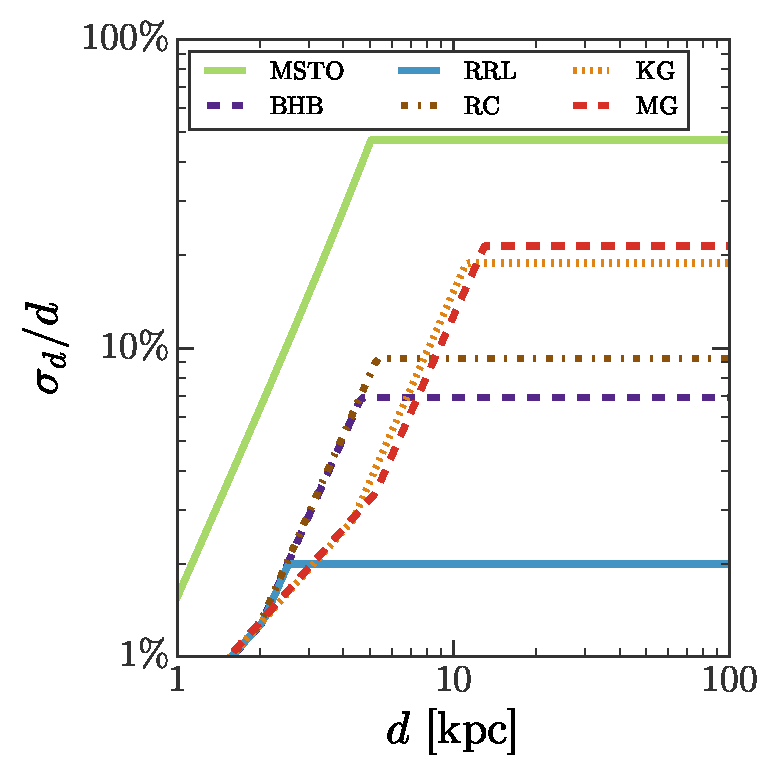
\includegraphics[width=0.48\textwidth]{figures/ch0/frac-plx-err.pdf}
    }
    \subfloat{
      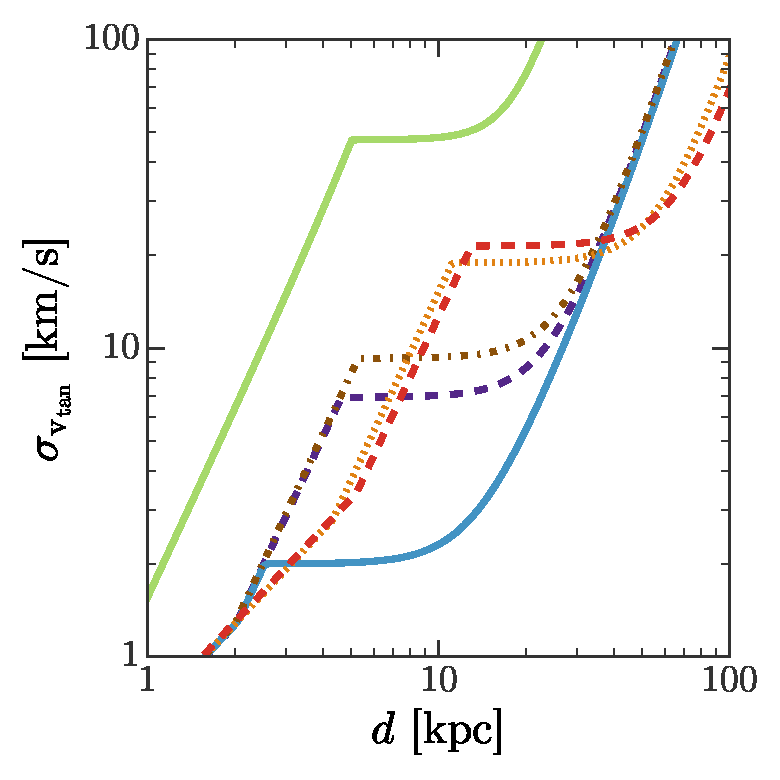
\includegraphics[width=0.48\textwidth]{figures/ch0/vtan-err.pdf}
    }
\caption{Estimates for the astrometric precision of the end-of-mission data release from the \gaia\ mission for individual stars of different types. \textit{Left}: Fractional parallax or distance uncertainty for different stellar tracers as a function of distance. When the \gaia\ parallax uncertainty becomes larger than the distance uncertainty for an alternate distance measurement method, the minimum uncertainty is assumed. For example, for RR Lyrae (RRL) stars, distance measurements from the period-luminosity relation are $\approx$2\%. For other stars, photometric distance uncertainties range from $\approx$8--50\%. \text{Right}: Tangential velocity uncertainty using the fractional distance uncertainties in the left panel and the proper motion uncertainties from \gaia\ for a star with a tangential velocity $v_{\rm tan} = 100~\kms$.}
\label{fig:gaiastellarpops}
\end{figure}

The \gaia\ mission is currently measuring parallaxes, proper motions, and radial
velocities for $\approx$$10^{8}$ stars in the Milky Way. The end-of-mission data
release from \gaia\ (expected in 2022) will provide astrometric measurements for
$\approx$$10^{9}$ stars. At distances $\gtrsim$10 kpc in the \mwhalo, the radial
velocity and parallax uncertainties will be large for all stellar types, but the
proper motion uncertainties will still be useful.
Figure~\ref{fig:gaiastellarpops} shows a summary of the expected distance and
tangential velocity uncertainties for each of the stellar tracers reviewed in
the previous section. Of particular note are the RR Lyrae stars, which will have
precise distance measurements and tangential velocity uncertainties
$\lesssim$$10~\kms$ out to 25 kpc.

Another highly anticipated survey for Milky Way \mwhalo\ science is the Large
Synoptic Survey Telescope \citep[LSST;][]{lsstsciencebook}. The telescope design
and large mirror of the LSST will enable deep imaging over a huge field of view
(magnitude limits of $\approx$24.5 for single-epoch images, $\approx$27.5 for
coadded images). The LSST will image most of the visible sky in five filters
every few nights, which will allow identification of faint time-variable stars
like RR Lyrae stars at extreme distances (out to $\approx$2--3 times the virial
radius of the Milky Way). At the faint end, the LSST will supercede the \gaia\
astrometry and provide proper motions better than $\lesssim$$1~{\rm mas}~{\rm
yr}^{-1}$ for stars with $r$-band magnitudes $20 \lesssim r \lesssim 24$. The
survey will begin science operations in 2022 with the first data release
expected about a year later.

Much of the \mwhalo\ will be mapped in sky position, distance, and proper motion
by the combination of \gaia\ and LSST; the last kinematic quantities needed are
radial velocities. Unlike multi-object spectroscopy---needed to obtain large
samples of radial velocities---imaging surveys do not scale in complexity with
the number of sources. Robotic fiber-positioner spectrographs
\citep{saunders12} have and will make it possible to simultaneously observe
1000s of stars, but are expensive to maintain and don't scale much above this
number. Combined with the longer exposure times needed to obtain high
signal-to-noise spectra, obtaining spectroscopy for a volume of stars comparable
to the astrometric sources in \gaia\ will be an enormous technological
challenge. However, it will be necessary in order to fully map out the
chemical-abundance structure of and measure radial velocities for these sources.
Many ongoing efforts \citep[e.g.,][]{rave06, segue08, apogee15, galah15} have
obtained spectra of varied resolution for $\approx$1 million stars around the
Galaxy. The future Dark Energy Spectroscopic Instrument
\citep[DESI;][]{desi-whitepaper} will take spectra of an additional
$\approx$$10^7$ stars, but this is still orders of magnitude below the number
needed to have complete 6D phase-space coverage for the entire Milky Way halo.

% [...maybe add something about focusing on particular tracer?]

\section{Outline of thesis}

Rich kinematic data impending, what can we learn about the dark matter halo of the Milky Way?

\todo{stuff}

	\chapter[Spitzer, Gaia, and the Potential of the Milky Way]{Spitzer, Gaia, and the Potential of the Milky Way}\label{ch:rewinder1}
\let\thefootnote\relax\footnotetext{This section contains text from an article published in The Astrophysical Journal Letters, Volume 778, Issue 1, article id. L12, 6 pp. (2013). Portions of this paper's introduction now appear in the introduction to this dissertation.}

\renewcommand{\article}{\emph{Chapter}}

%\documentclass{emulateapj}
%%\documentclass[preprint]{aastex}
%
%%\documentclass{aastex}
%%\usepackage{emulateapj5}
%%\usepackage{lscape}
%\usepackage{natbib}
%\usepackage{amssymb,amsmath}
%\usepackage{hyperref}
%
%% Convenience
%\newcommand{\bs}{\boldsymbol}
%\newcommand{\argmin}{\operatornamewithlimits{argmin}}
%
%\setlength{\jot}{12pt}
%
%\begin{document}
%\submitted{Accepted to ApJ Letters}
%\title{Spitzer, Gaia, and the Potential of the Milky Way}
%
%\author{Adrian~M.~Price-Whelan\altaffilmark{1,2} Kathryn V. Johnston\altaffilmark{1}}
%
%% affiliations
%\altaffiltext{1}{Department of Astronomy, Columbia University, 550 W 120th St., New York, NY 027, USA}
%%\altaffiltext{2}{NSF Graduate Fellow}
%\altaffiltext{2}{\email{adrn@astro.columbia.edu}}
%
%\begin{abstract}
%
%Near-future data from ESA's {\it Gaia} mission will provide precise, full phase-space information for hundreds of millions of stars out to heliocentric distances of $\sim$10 kpc. This ``horizon'' for full phase-space measurements is imposed by the {\it Gaia} parallax errors degrading to worse than 10\%, and could be significantly extended by an accurate distance indicator. Recent work has demonstrated how {\it Spitzer} observations of RR Lyrae stars can be used to make distance estimates accurate to 2\%, effectively extending the {\it Gaia}, precise-data horizon by a factor of ten in distance and a factor of 1000 in volume. This \emph{Letter} presents one approach to exploit data of such accuracy to measure the Galactic potential using small samples of stars associated with debris from satellite destruction. The method is tested with synthetic observations of 100 stars from the end point of a simulation of satellite destruction: the shape, orientation, and depth of the potential used in the simulation are recovered to within a few percent. The success of this simple test with such a small sample in a single debris stream suggests that constraints from multiple streams could be combined to examine the Galaxy's  dark matter halo in even more  detail --- a truly unique opportunity that is enabled by the combination of {\it Spitzer} and {\it Gaia} with our intimate perspective on our own Galaxy.
%
%\end{abstract}
%
%\keywords{
%  Galaxy: structure
%  ---
%  Galaxy: halo
%  ---
%  cosmology: dark matter
%}

\newcommand{\argmin}{\rm argmin}

\section{Introduction}
\label{intro.sec}
The existence of vast halos of unseen {\it dark} matter surrounding each galaxy has long been proposed to explain the surprisingly large
motions of the {\it baryonic} matter that we can see \citep[e.g.,][]{rubin70}.
Dark-matter-only simulations of structure formation lead us to expect that these dark matter halos should have density distributions that are described by a universal radial profile \citep{navarro96} with a variety of triaxial shapes \citep{jing02}.
The inclusion of baryons in the simulations tends to soften the triaxiality of the dark matter in the inner regions of the halo \citep[e.g., as the disk forms,][]{bailin05} and
can alter the radial profile through a combination of adiabatic contraction and energetic feedback \citep[e.g.][]{pontzen12}.
Hence, measurements of the shape, orientation, radial profile, and extent of dark matter halos provides information about the formation of these vast structures, as well as the messy baryonic processes that continue to shape them.

The Milky Way is the best candidate for such a detailed study of a dark matter halo
since we can resolve large samples of stellar tracers.
Thousands of blue horizontal branch stars selected from the Sloan Digital Sky Survey (SDSS) have been used to probe the Milky Way mass out to tens of
kpc \citep[SDSS, see][]{deason12a,kafle12}, and estimates with combined tracers extend to 150 kpc \citep{deason12b}.

This approach assumes that the tracers represent a random sampling of phase-mixed orbits drawn from a smooth distribution function, however large area surveys have revealed the existence of large-scale spatial inhomogeneities in the form of giant stellar streams \citep{newberg02,majewski03,belokurov06}, demonstrating that a significant fraction of the stellar halo is neither randomly sampled nor is fully phase-mixed.

%A complimentary approach to measuring the mass distribution is to instead take advantage of the {\it non}-random nature of the Galaxy's stellar distribution and utilize the knowledge that stars in streams were once all part of the same object.
%Such approaches can require orders of magnitude fewer tracers than a randomly sampled population to achieve comparable accuracy.
%One method is to simply fit orbits to observations of streams 
%\citep[e.g.,][]{koposov10}.
%However, the assumption that debris traces a single orbit is actually incorrect \citep[see][]{johnston98,helmi99} and
%changes in orbital properties along debris streams can lead to systematic biases in measurements of the Galactic potential \citep{eyre09a,varghese11}.
%\citet{sanders13a} recently demonstrated that this bias is equally problematic for the very thinnest, coldest streams, whose observed properties may be indistinguishable from those of the parent orbit \citep[e.g. such as the globular cluster, GD1 --- see][]{koposov10}, as for the much more extended and hotter streams \citep[e.g. such as debris from the Sagittarius dwarf galaxy --- see][]{majewski03} where offsets from a single orbit are clearly apparent.
%
%One way to address these biases is to run self-consistent N-body simulations of satellite destruction in a variety of potentials with the aim of simultaneously constraining both the properties of the satellite and the Milky Way.
%Many studies of the Sagittarius debris system (hereafter Sgr) have adopted this approach,
%with the most recent work attempting to place constraints on the triaxiality and orientation of the dark matter halo
%\citep{law10}.
%
%The promise of near-future data sets including full phase-space information has also inspired other approaches. \citet{binney08} and \citet{penarrubia12} demonstrate that the distribution of energy and entropy in debris, respectively, will be minimized only for a correct
%assumption of the form of the Galactic potential.
%\citet{sanders13b} examine the distribution of debris in action-angle co-ordinates and show that stars stripped from the same disrupted object must lie along a single line in angle-frequency space, providing a constraint that can be used as a potential measure.

In this \article\ we re-examine and update a complimentary approach that uses tidal debris as a potential measure \citep[originally proposed by][]{johnston99a} in the context of current and near-future observational capabilities, and apply it to a simulation of the Sagittarius debris system (hereafter Sgr).
In Section \ref{sec:context} we outline the observational prospects and Sgr properties that motivated this re-examination.
In Section \ref{sec:method} we present the updated potential measure and test it with synthetic observations of simulated Sgr debris.
In Section \ref{sec:discussion} we highlight the advantages and shortcomings of this method.
We conclude in Section \ref{sec:conclusion}.

\section{Context and motivation} \label{sec:context}
The method presented in Section \ref{sec:method} takes advantage of
three distinct developments: (i)
the demonstration of a technique for deriving distances to individual
RR Lyrae stars with 2\% accuracies (Section \ref{sec:spitzer}); (ii)
the prospect of proper motion measurements of the same stars with
$\sim$10~$\mu$as/yr precision (Section \ref{sec:gaia}); and (iii) the
tracing of debris associated with Sgr around the entire Galaxy
(Section \ref{sec:sgr})

\subsection{{\it Spitzer} and 2\% distance errors to RR Lyrae in the halo}
\label{sec:spitzer}

There is a long tradition for using RR Lyrae stars in the Galaxy to
study structure 
\citep[e.g.][]{shapley18}, substructure
\citep[e.g.][]{sesar10}, and distances to satellite galaxies
\citep[e.g.][]{clementini03}.  However, studies of RR Lyrae at optical
wavelengths are limited by both metallicity effects on the intrinsic
brightness of these stars and variable extinction along the line of
sight.  Moreover, systematic differences between instruments make it
difficult to tie observations across the sky to a common scale. 

At longer wavelengths, RR Lyrae promise tighter constraints on
distances.  
\citet{madore12} have recently shown, 
using five stars with
trigonometric parallaxes measured by Hubble \citep{benedict11},
that the dispersion in the mid-IR Period-Luminosity (PL) relation 
\citep[first mapped by][]{longmore86}
at
wavelengths measurable by NASA's {\it Spitzer} mission is $\sim$0.03~mag.
This implies that it is
possible to use {\it Spitzer} to determine distances that are good to $2\%$ for 
individual RR Lyrae stars out to $\sim$60~kpc ({\it Spitzer}'s limit for detecting and measuring RR Lyrae).
For comparison, distance measurements of Blue Horizontal Branch
stars typically
achieve $\sim$10-15\% uncertainties  \citep[if appropriate color measurements are available, e.g.,][]{deason12b}.

\begin{figure}[hp!]
\begin{center}
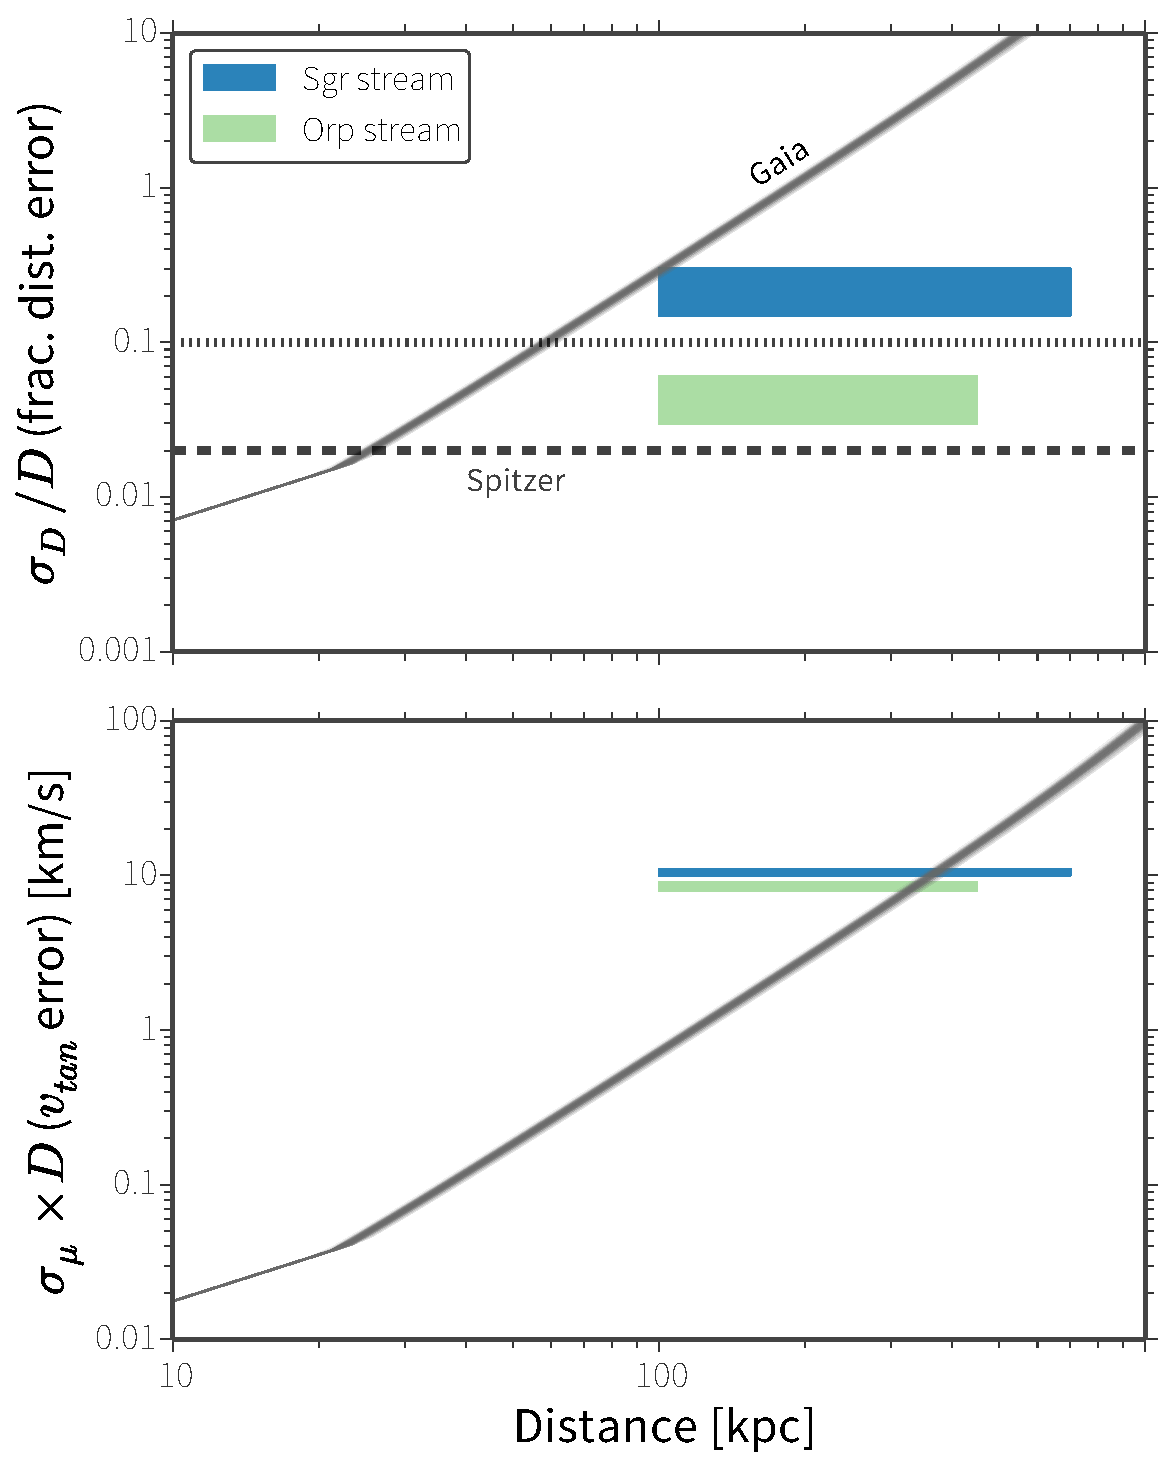
\includegraphics[width=0.7\textwidth]{figures/ch1/fig1.pdf}

\caption{Expected {\it Gaia} distance and tangential velocity errors as a function of heliocentric distance for RR Lyrae stars. Errors are a function of color and magnitude of the source, and hence the metallicity: each line is computed
by Monte Carlo sampling from the empirical metallicity distribution of
the Galactic halo from \cite{ivezic08}. Parallax distance errors from {\it Gaia} are larger than the line-of-sight size of both Sgr and Orphan (Orp), but photometric distance errors are comparable to the the Sgr scale (assuming 10\% errors, dotted line). Bottom panel shows that the {\it Gaia} tangential velocity errors are smaller than the internal velocity dispersion of nearer regions of both Sgr and Orp. }\label{fig:gaia_errors}
\end{center}
\end{figure}

\subsection{Gaia and the age of astrometry}
\label{sec:gaia}
The {\it Gaia} satellite \citep{gaia01} is
an astrometric mission which aims to measure the positions of billions
of stars with 10-100~$\mu$as accuracies. Combined with expected 
proper motion accuracies, this will enable full six-dimensional phase-space 
maps of the Galaxy with $<$10\% distance errors for heliocentric distances of
up to $\sim$6~kpc for RR Lyrae stars.

Figure~\ref{fig:gaia_errors} shows the {\it Gaia} end-of-mission distance
and tangential velocity error estimates for RR Lyrae. Within 2~kpc, {\it Gaia} will measure distances to these stars with
better than 2\% accuracy --- RR Lyrae in this volume can be used to
test and calibrate the {\it Spitzer} PL relation described above. Beyond the
2~kpc threshold, the mid-IR PL relation for RR Lyrae will provide better 
distance measurements. 

The combination of {\it Spitzer} and {\it Gaia} data will 
extend the ``horizon'' of where precise, six-dimensional phase-space 
maps of the Galaxy are possible from $<$10~kpc to 60~kpc. This enormous 
increase in volume will greatly refine data on debris systems in the halo.

\subsection{The Sagittarius debris system}
\label{sec:sgr}
Sgr was discovered serendipitously during a radial velocity 
survey of the Galactic bulge \citep{ibata94}. 
Signatures of extensive stellar
streams associated with Sgr have since  been
mapped across the sky in carbon stars \citep{totten98}, M giants
selected from 2MASS \citep{majewski03}, main
sequence turnoff stars from SDSS
\citep{belokurov06}, and RR Lyrae in the Catalina Sky Survey
\citep{drake13}. 

Sgr stream data has inspired a rich set of  models 
\citep[e.g.,][]{johnston99b, fellhauer06}.
Most recently, \citet[][hereafter LM10]{law10} combined all
the (then) current data on the Sgr debris to constrain both a model of its evolution
and the potential in which it orbits. (Note that new observational work by 
\citet{belokurov13} suggest that the trailing tail of Sgr debris does not
match the LM10 model.)
Figure \ref{fig:lm10} shows particle positions
from the final time-step of the LM10 N-body
simulation of dwarf satellite disruption along the expected Sgr orbit
in the best-fitting Milky Way halo model. The simulation was
run in a three-component potential, with a triaxial, logarithmic halo
model of the form
\begin{equation}
  \Phi_{halo} = v_{halo}^2 \ln(C_1 x^2 + C_2 y^2 + C_3 xy + (z/q_z)^2 + R_c^2)
\end{equation}
where $C_1$, $C_2$, and $C_3$ are combinations of the $x$ and $y$ axis
ratios ($q_1$, $q_2$) and orientation of the halo with respect to the
baryonic disk ($\phi$):
\begin{align}
  C_1 &= \frac{\cos^2\phi}{q_1^2} + \frac{\sin^2\phi}{q_2^2}\\
  C_2 &= \frac{\sin^2\phi}{q_1^2} + \frac{\cos^2\phi}{q_2^2}\\
  C_3 &= 2\sin\phi\cos\phi \left(q_1^{-2} - q_2^{-2}\right).
\end{align}

\begin{figure}[t]
\begin{center}
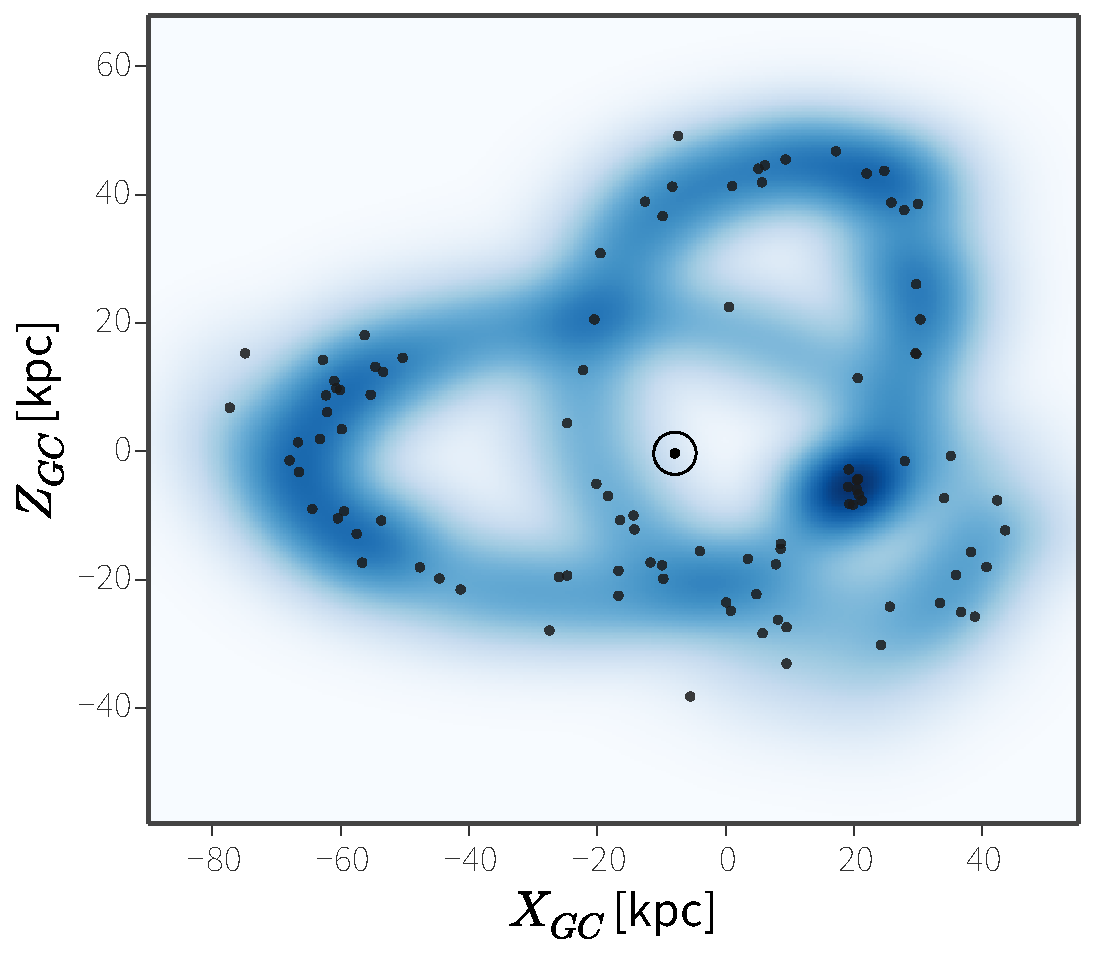
\includegraphics[width=0.7\textwidth]{figures/ch1/fig2.pdf}
\caption{ Particle density (blue) of the first leading and trailing wraps from the final time-step of the \citet{law10} simulation of the Sgr stream. Point markers (black) show positions of a random sample of 100 stars drawn from this density distribution. The position of the Sun is shown with the solar symbol. }\label{fig:lm10}
\end{center}
\end{figure}

%LM10 demonstrate how a comparison of such simulations with the observed debris enables a detailed reconstruction of Sgr's history: its mass and stellar populations, orbit, rate of destruction, and even original distribution in populations. 
A comparison of simulations and data enabled LM10 to make an assessment of the three-dimensional 
mass distribution of the Milky Way's dark matter
halo through constraints on the potential parameters $v_{\rm halo}$, $q_1$, $q_z$, and $\phi$. Combined {\it Spitzer} and {\it Gaia} measurements of distances and proper motions
of RR Lyrae in the Sgr debris will open up new avenues for potential constraints. Figure~\ref{fig:gaia_errors} shows that a 2\% distance error is smaller than the 
distance range in the stream (top panel). Similarly, {\it Gaia} proper motion
error estimates correspond to tangential velocity errors less than the velocity
dispersion for much of the stream (bottom panel). The next section outlines a 
new method to take advantage of this information. 

%A 2\% distance error at $\sim$30~kpc
%($\epsilon_{d}=0.6~{\rm kpc}$) is smaller than the predicted thickness
%of the stream ($\sim$2-$10$~kpc). When combined with {\it Gaia} proper motion errors,
%tangential velocity measurement accuracies ($\epsilon_{v}\sim2$~km/s
%at 30~kpc; see Figure~\ref{fig:gaia_errors}) are less than the intrinsic dispersion for much of the stream
%\citep[$\sigma_v\sim10$~km/s;][]{majewski04}. The next section
%outlines a new method to take advantage of this information.

\section{Description and test of our algorithm}
\label{sec:method}
With access to 6D information for stars in a tidal
stream, each star becomes a powerful potential
measure by exploiting the fact that the stars must have come from the
same progenitor: if the orbits of the stars and progenitor are integrated 
\emph{backwards} in a a potential that accurately models the Milky Way, the stars
should recombine with the progenitor (imagine watching satellite destruction in ``rewind"). If the potential is incorrect,
the orbits of the stars will diverge from that of the progenitor and
thus will not be recaptured by the satellite system (Figure~\ref{fig:ps_distance}).

This approach was originally proposed by \citet{johnston99a} and was tested on the proposed characteristics of the Space
Interferometry Mission \citep{unwin08}. Below we present an updated version of the algorithm:
the promise of 2\% distances to RR Lyrae stars (see Section
\ref{sec:spitzer}) enables a direct measurement (rather than
approximate estimate, as previously assumed) of the position of a star within its debris
structure. The test statistic that quantifies how well stars recombine
with the satellite has also been rigorously redefined.

\begin{figure}[hp!]
\begin{center}
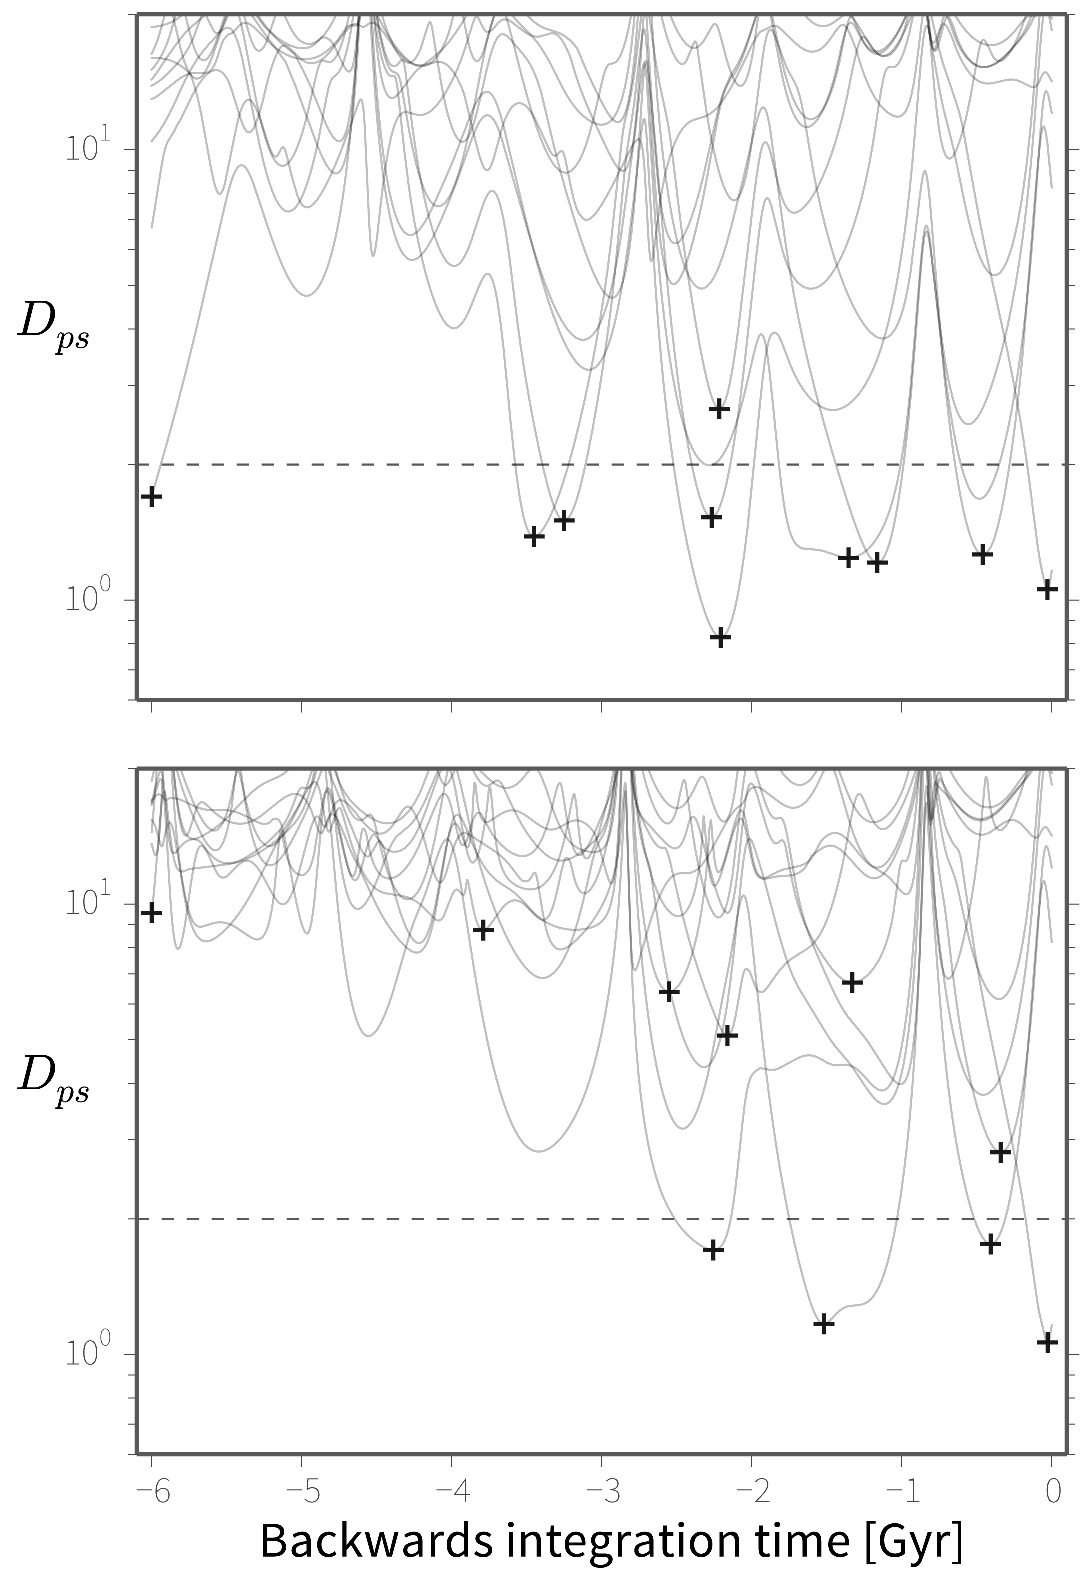
\includegraphics[width=0.7\textwidth,trim=5 0 0 0, clip]{figures/ch1/fig3.pdf}
\caption{Phase space distance ($D_{\rm ps}$) for 10 randomly selected stars integrated backwards in the correct potential (top) and a potential where $q_z$ is 25\% larger (bottom). The same 10 particles are used in both figures, so the initial conditions are identical. Horizontal (dashed) line shows $D_{\rm ps}=2$, for reference.}\label{fig:ps_distance}
\end{center}
\end{figure}

\subsection{The algorithm: Rewinder}
Quantifying this method requires a sample of stars with known full
space kinematics $(\bs{x}_{i}, \bs{v}_{i})|_{t=0}$ (e.g., measurements
of all position and velocity components for these stars \emph{today}
at $t=0$), the orbital parameters for the progenitor system
$(\bs{x}_p, \bs{v}_p)|_{t=0}$, and a functional form for the
potential, $\Phi({\boldsymbol\theta})$. For a given set of potential
parameters, $\boldsymbol\theta$, the orbits of the stars and
progenitor are integrated backwards for several Gigayears. At
each timestep $t_j$, for each particle $i$, a set of normalized,
relative phase-space coordinates are computed
\begin{equation}
  \bs{q}_{i} = \frac{\bs{x}_{i} -
    \bs{x}_{p}}{R_{\rm tide}}\,\,\,\,,\,\,\,\,\bs{p}_{i} = \frac{\bs{v}_{i} -
    \bs{v}_{p}}{v_{\rm esc}}
\end{equation}
where $(\bs{x},\bs{v})_{i}$ and $(\bs{x},\bs{v})_{p}$ are the
phase-space coordinates for the particles and progenitor,
respectively. These definitions require an estimate of the mass of the
satellite, $m_{sat}$, which, combined with the orbital radius of the
satellite, $R$, and the computed enclosed mass of the potential within
$R$, $M_{enc}$, sets the instantaneous tidal radius and escape
velocity,
\begin{equation}
  R_{\rm tide}=R\Big(\frac{m_{\rm sat}}{3M_{\rm enc}}\Big)^{1/3}\,\,\,\,,\,\,\,\,
  v_{\rm esc}=\sqrt{\frac{2Gm_{\rm sat}}{R_{\rm tide}}}.
\end{equation}
These quantities are computed at each time step to take the time 
dependence into account, neglecting mass-loss from the satellite.
Qualitatively, when the distance in this normalized six-dimensional
space, $D_{{\rm ps},i}=\sqrt{|\bs{q}_{i}|^2+|\bs{p}_{i}|^2} \lesssim 2$, 
the star is likely recaptured by the satellite (in the absence of errors,
 we find that $\sim$90\% of the initially bound particles come within
 this limit when integrating all orbits backwards). \citet{johnston99a} 
 imposed a similar condition as a hard boundary and maximized the 
number of recaptured particles in a given backwards-integration.
What follows is a description of an updated procedure with a 
statistically-motivated choice for an objective function.

For each star, $i$,
the phase-space distance, $D_{\rm ps}$, is computed at each timestep
$t_{j}$, and the vector with the minimum phase-space distance is stored
\begin{align}
  t^*_{i} &= \argmin_{t} D_{{\rm ps},i}\\
  \bs{A}_{i} &= (\bs{q}_{i}(t^*_{i}),\bs{p}_{i}(t^*_{i})).
\end{align}
Thus, the matrix $\bs{A}_{ik}$ contains these minimum phase-space
distance vectors for each star, where $k\in[1,6]$. Intuitively, the
variance of the distribution of minimum phase-space vectors will be
larger for orbits integrated in an incorrect potential relative to the
distribution computed from the `true' orbital history of the stars: in
an incorrect potential, the orbits of the stars relative to the orbit of 
the progenitor spread out in phase space. Thus, the \emph{generalized
 variance} of the distribution --- computed for a given set of
potential parameters, $\bs{\theta}$ --- is a natural choice for the
scalar objective function, $f(\bs{\theta})$, used in constraining the potential of the
Milky Way
\begin{align}
  \Sigma_n &= \mathrm{Cov}( \bs{A}_{ik}) \\
  f(\bs{\theta}) &= \ln \det \Sigma_n.
\end{align}

\subsection{Application to Simulated Data} \label{sec:results}
The LM10 simulation data (see Section \ref{sec:sgr}) is a perfect
test-bed for evaluating the effectiveness of this method. We start by
extracting both particle data and the satellite orbital parameters
from the present-day snapshot of the simulation
data.\footnote{\url{www.astro.virginia.edu/~srm4n/Sgr/data.html}} We
then ``observe'' a sample of 100 stars from the first leading and
trailing wraps of the stream. The radial velocity and distance errors are drawn 
from Gaussians ($\varepsilon_{\rm RV} \sim \mathcal{N}(\mu=0,\sigma=10~{\rm
  km/s})$ and $\varepsilon_{\rm D} \sim \mathcal{N}(0,0.02\times
D)$) and the proper motion errors are computed from the expected {\it Gaia} error curve.\footnote{\url{http://www.rssd.esa.int/index.php?page=Science_Performance&project=GAIA}} 

The generalized variance defines a convex function over
which we optimize four of the six logarithmic potential parameters:
$v_{circ}$, $\phi$, $q_1$, and $q_z$ ($q_2$ and $R_c$
are degenerate with combinations of the other parameters). 
Figure~\ref{fig:objective} shows one-dimensional slices of
the objective function produced by varying each of the potential
parameters by $\pm10\%$ around the true values and holding all others
fixed.

\begin{figure}[t]
\begin{center}
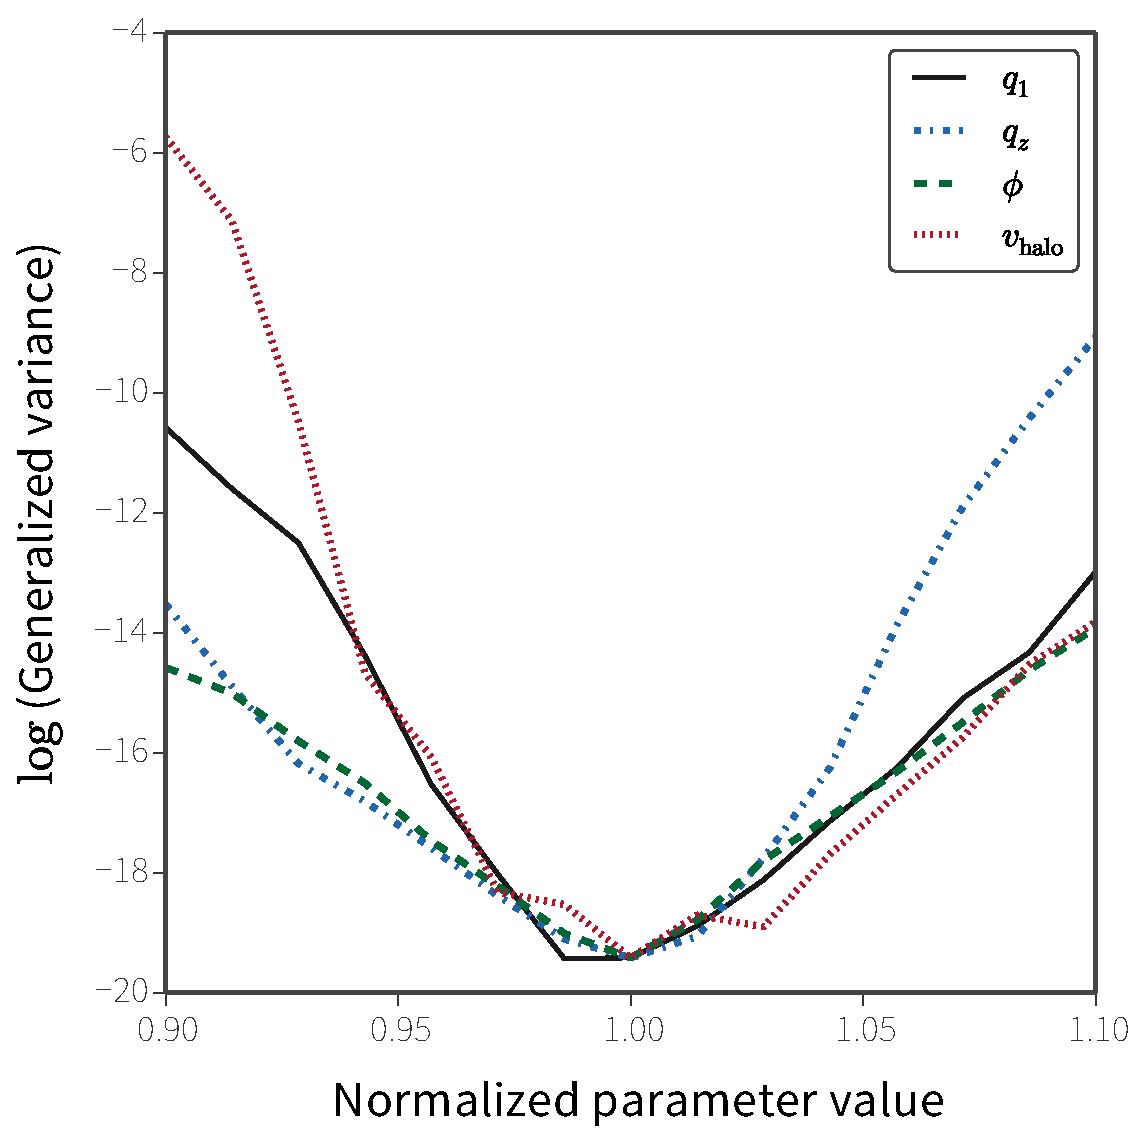
\includegraphics[width=0.5\textwidth]{figures/ch1/fig4.pdf}
\caption{ 1D slices of the objective function (generalized variance) for each halo potential parameter. The parameter values are normalized by the true values show the effect of varying each parameter by $\pm10$\%. The values of the objective function (vertical axis) are not interesting but note the minima around the truth (1.0).}\label{fig:objective}
\end{center}
\end{figure}

\begin{figure*}[t]
\centering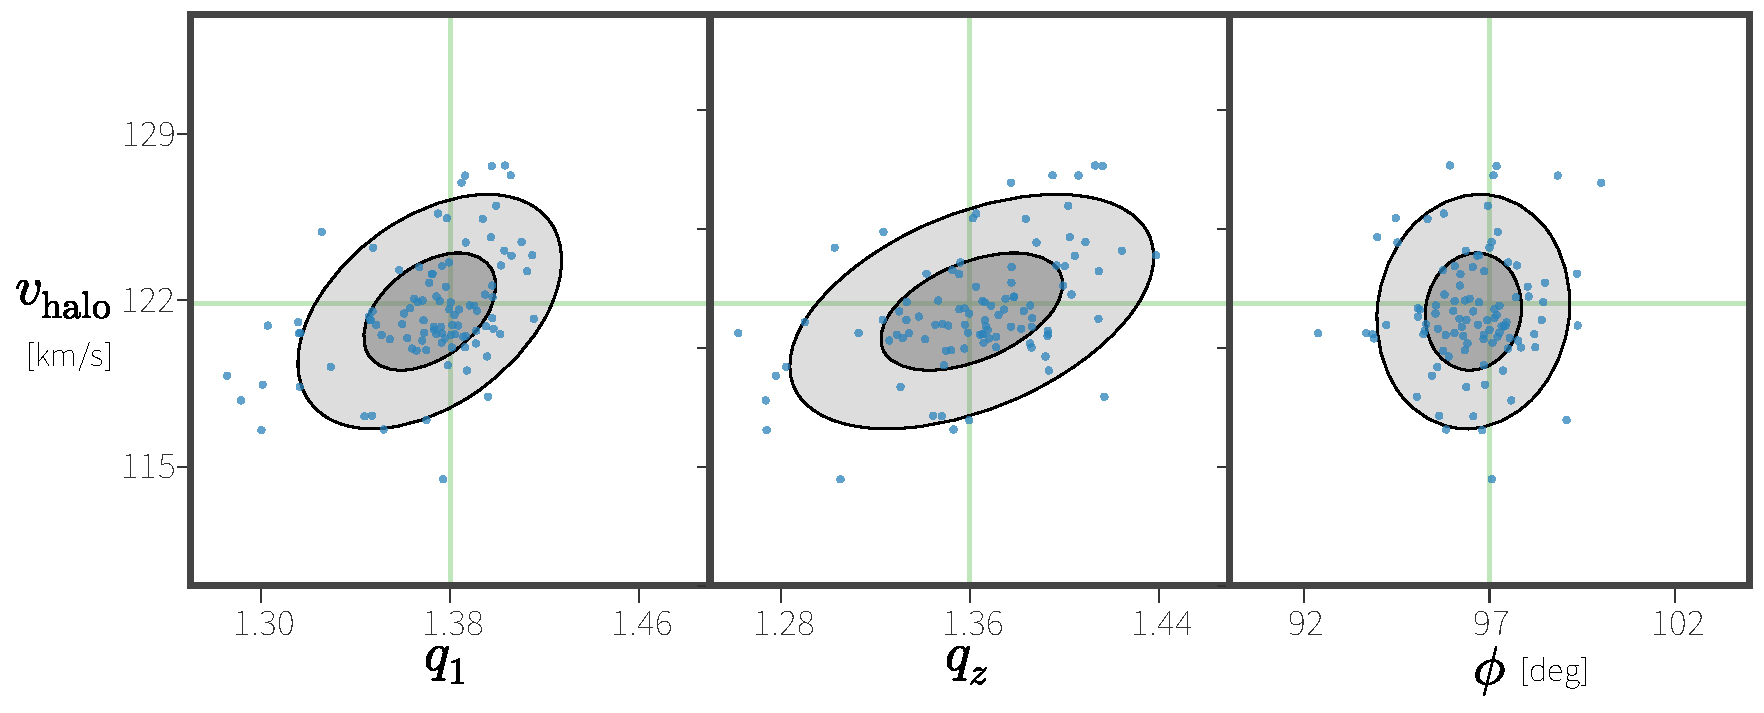
\includegraphics[width=0.9\textwidth,trim=0 0 0 0, clip]{figures/ch1/fig5.pdf}
\caption{ Blue points show the ``best-fit'' parameters resulting from each resample of 100 stars from the Sgr stream particle density shown in Figure~\ref{fig:lm10}. Green (vertical and horizontal) lines show the true values of the parameters. Grey ellipses show one- and two-sigma margins, assuming the points are normally distributed. }\label{fig:bootstrap}
\end{figure*}	

In anticipation of extending the above method to include a true
likelihood function, we use a parallelized Markov Chain Monte Carlo
(MCMC) algorithm \citep{foremanmackey2013} to sample from our
objective function.\footnote{Though MCMC is typically not an efficient
  optimization tool, in this case objective function is both noisy and
  expensive to compute. The stochasticity and easy parallelization of
  the algorithm outperforms other optimizers on this problem.}
We use the median value of the converged sample distribution as a
point estimate for the potential parameters. To assess the uncertainty
in the derived halo parameters, we sample 100 stars
100 times and estimate the potential parameters with each
resampling. Figure~\ref{fig:bootstrap} shows the recovered parameters
for each sample and demonstrates the power of this method:
a moderately sized sample of RR Lyrae
alone places strong constraints on the shape and mass of the
Galaxy's dark matter halo. From the covariance matrix derived from the 
distribution of points in Figure~\ref{fig:bootstrap}, we find the mean 
recovered parameters and one-sigma deviations to be 
$q_1 = 1.36 \pm 0.02$, $q_z = 1.36 \pm 0.03$, $\phi = 96.0 \pm 1.5$ degrees,
and $v_{\rm halo} = 123.2 \pm 1.6$ km/s.

\section{Discussion, strengths, and limitations}
\label{sec:discussion}

The strengths of this method stem from its simplicity: it requires
only a rough estimate of the satellite mass $m_{\rm sat}$ combined
with backwards integration of orbits. 
\emph{Rewinder} does not assume that stream stars follow
a single orbit and instead \emph{relies}
on the fact that each star is on a different orbit. There are also no assumptions made
about of the internal distribution of satellite
stars. Thus, \emph{Rewinder} is applicable to any debris that is
known to come from a single object and not restricted to the coldest
tidal streams. In principle, it could also be applied to the
vast stellar debris {\it clouds} that have been discovered 
\citep[e.g., the Triangulum-Andromeda and Hercules-Aquila
  clouds;][]{rochapinto04,belokurov06}, or even stars that have only
associations in orbital properties and do not form a coherent spatial
structure \citep[e.g.][]{helmi99}. The method trivially extends to
combining constraints from multiple debris systems at once by simply
integrating all debris from several satellites simultaneously, with
$D_{\rm ps}$ defined appropriately for each star.

It is also important to characterize the the limitations of this
method. Firstly, the measurement errors for RR Lyraes associated with
the very coldest streams \citep[e.g., the globular clusters Pal5 and
  GD1;][]{odenkirchen02,koposov10} will likely be too large to resolve
the minute differences in orbital properties between the debris and
satellite. Second, the present prescription neglects orbital evolution (e.g.,
dynamical friction) and scattering of stream stars due to the potential
of the satellite. Preliminary simulations (to be fully explored in 
forthcoming work) suggest that these two points can be neglected 
for satellite masses between $\sim$$10^7$ and $\sim$$10^9~\mathrm{M}_{\odot}$. Lastly, the 
current version of the algorithm relies on knowledge of the current 
position and velocity of the parent satellite, which may not be available 
\citep[e.g., the Orphan Stream;][]{belokurov07}. 

\section{Conclusions and motivation for future work}
\label{sec:conclusion}

This paper presents an algorithm for measuring the Galactic potential
that anticipates combined data from the {\it Spitzer} and {\it Gaia} satellite
missions which promise precise, full phase-space measurements of RR
Lyrae stars in the halo of our Galaxy. When applied to a sample of 100
stars (with realistic observational errors) drawn from the
\cite{law10} N-body simulation of the destruction of the Sgr dwarf
satellite, \emph{Rewinder} recovers the depth, shape, and orientation of the dark
matter potential to within a few percent.

While the tests presented in this paper are very simple, the accuracy of potential recovery promised by such a small sample of stars 
provides strong motivation for further theoretical work to: 1) develop a robust generative model that utilizes the concepts demonstrated by \emph{Rewinder}; 2) investigate the power of using multiple debris structures; and 3) examine how \emph{Rewinder} might work with less accurate measurements or missing dimensions. 

Our results also motivate an observational campaign with {\it Spitzer} to survey RR Lyrae stars in debris structures around the Milky Way to get precise distances to combine with near-future {\it Gaia} velocity data. 
If just 100 stars in a single stellar stream allow us to study the depth, shape, and orientation of the Milky Way potential, larger samples in multiple structures \citep[e.g., the Orphan Stream;][]{sesar13} offer the prospect of assessing these quantities as a function of Galactocentric radius. Tracing the mass in a dark matter halo with this level of detail is impossible for any other galaxy in the Universe.

\section*{Acknowledgments}
We thank Barry Madore for providing the inspiration for this work. Thanks to 
David Hogg for statistical advice. Thanks also to Steve Majewski, David 
Law, and David Nidever. We also thank the anonymous referee for useful 
suggestions. 

APW is supported by a National Science Foundation Graduate Research
Fellowship under Grant No.\ 11-44155. This work was supported in part by 
the National Science Foundation under Grant No. PHYS-1066293 and the 
hospitality of the Aspen Center for Physics.

	\chapter[Inferring the gravitational potential of the Milky Way with a few
precisely measured stars]{Inferring the gravitational potential of the Milky Way
with a few precisely measured stars \label{ch:rewinder2}}
\let\thefootnote\relax\footnotetext{This section contains text from an article
published in The Astrophysical Journal, Volume 794, Issue 1, article id. 4, 15
pp. (2014). Portions of this paper's introduction now appear in the introduction
to this dissertation.}

% More definitions for this chapter
\newcommand{\D}{{\bf D}}
\newcommand{\W}{{\bf W}}
\newcommand{\X}{{\bf X}}
\newcommand{\J}{{\boldsymbol J}}
\newcommand{\bSigma}{{\bf \Sigma}}
\newcommand{\bsigma}{\boldsymbol\sigma}
\newcommand{\rtide}{r_{\rm tide}}
\newcommand{\sat}{{\rm p}}
\newcommand{\tub}{t_{\rm ub}}
\newcommand{\tint}{t_{\rm int}}
\newcommand{\rr}{\widetilde{\bs{r}}}
\newcommand{\vv}{\widetilde{\bs{v}}}
\newcommand{\tailbit}{\beta}
\newcommand{\Loffset}{\alpha}
\newcommand{\pshock}{P_{\rm shock}}
\newcommand{\paperone}{Paper 1}
\newcommand{\vhalo}{v_{\rm h}}
\newcommand{\rhalo}{r_{\rm h}}
\newcommand{\potp}{$q_1,q_z,\phi,\vhalo,\rhalo$}

%\begin{document}
%
%\title{Inferring the gravitational potential of the Milky Way with a few precisely measured stars}
%\author{Adrian M. Price-Whelan\altaffilmark{\colum,\adrn},
%	    David W. Hogg\altaffilmark{\nyu,\cds,\mpia},
%	    Kathryn V. Johnston\altaffilmark{\colum},
%	    David Hendel\altaffilmark{\colum}}
%
%% Affiliations
%\newcommand{\colum}{1}
%\newcommand{\adrn}{2}
%\newcommand{\nyu}{3}
%\newcommand{\cds}{4}
%\newcommand{\mpia}{5}
%\altaffiltext{\colum}{Department of Astronomy,
%		              Columbia University,
%		              550 W 120th St.,
%		              New York, NY 10027, USA}
%\altaffiltext{\adrn}{To whom correspondence should be addressed: adrn@astro.columbia.edu}
%\altaffiltext{\nyu}{Center for Cosmology and Particle Physics,
%                      Department of Physics, New York University,
%                      4 Washington Place, New York, NY, 10003, USA}
%\altaffiltext{\cds}{Center for Data Science,
%                      New York University,
%                      4 Washington Place, New York, NY, 10003, USA}
%\altaffiltext{\mpia}{Max-Planck-Institut f\"ur Astronomie,
%                     K\"onigstuhl 17, D-69117 Heidelberg, Germany}
%
%\begin{abstract}
%% New abstract: The dark matter halo of the Milky Way is expected to be triaxial and filled with substructure. It is hoped that streams or shells of stars produced by tidal disruption of stellar systems will provide precise measures of the gravitational potential to test these predictions. We develop a method for inferring the Galactic potential with tidal streams based on the idea that the stream stars were once close in phase space. Our method can flexibly adapt to any form for the Galactic potential: it works in phase-space rather than action-space and hence relies neither on our ability to derive actions nor on the integrability of the potential. Our model is probabilistic, with a likelihood function and priors on the parameters. The method can properly account for finite observational uncertainties and missing data dimensions. We test our method on synthetic datasets generated from N-body simulations of satellite disruption in a static, multi-component Milky Way including a triaxial dark matter halo with observational uncertainties chosen to mimic current and near-future surveys of various stars. We find that with just four well-measured stream stars, we can infer properties of a triaxial potential with precisions of order 5-7 percent. Without proper motions we obtain 15 percent constraints on potential parameters and precisions around 25 percent for recovering missing phase-space coordinates. These results are encouraging for the eventual goal of using flexible, time-dependent potential models combined with larger data sets to unravel the detailed shape of the dark matter distribution around the Milky Way.
%% Context
%The dark-matter halo of the Milky Way is expected to be triaxial on large scales
%  and filled with substructure.
%It is hoped that streams or shells of stars produced by tidal disruption
%  of smaller galaxies or globular clusters will provide very precise measures of
%  the gravitational potential
%  to test these predictions.
%% Aims
%We develop a statistically justified method for inferring the gravitational potential
%  using precise measurements of stars in tidal streams
%  based on the idea that these stars
%  were close in phase space at some point in the past.
%Our method can flexibly adapt to any form for the Galactic potential.
%In particular, it works in phase-space rather than action-space and hence relies neither on
%our ability to derive actions nor on the
%assumption of integrability of the potential.
%% Methods:
%Our model is probabilistic, with a likelihood function and priors on the parameters.
%The method can properly account for both finite observational uncertainties
%  and missing data dimensions.
%We test our method on synthetic data sets generated from an N-body simulation
%of satellite disruption in a static, multi-component Milky Way including a triaxial dark matter halo.
%The mock data sets were generated with
%  observational uncertainties to mimic current and near-future surveys of various stars.
%% Results:
%We find that with just eight well-measured stream stars,
%  we can infer properties of a triaxial potential with precisions of order 5-7 percent.
%Without proper motions we find that these same stars provide 15 percent constraints on potential parameters
%  and precisions around 25 percent for recovering missing phase-space coordinates.
%These results are encouraging for the eventual goal of using more flexible, time-dependent potential models
%  combined with larger data sets to unravel the detailed shape of the dark matter distribution around the Milky Way.
%% Conclusions:
%% The method generalizes to encompass mixtures of independent debris structures
%%   or situations in which star membership in structures is unknown.
%
%\end{abstract}
%
%\keywords{
%  Galaxy: kinematics and dynamics
%  ---
%  Galaxy: halo
%  ---
%  cosmology: dark matter
%}
%
\section{Introduction}\label{sec:ch3-intro}

%Early large-scale, cosmological simulations of galaxy formation in the $\Lambda$CDM paradigm suggested that the spherically-averaged density profiles of dark matter halos follow a universal profile across a large dynamic range in mass \citep{navarro96}. Since then, higher resolution simulations --- both with and without baryons --- have produced dark matter halos that (1) are permeated with substructure on many scales, (2) are triaxial in shape, and (3) have shapes and orientations that vary with radius \citep{dubinski91, jing02, kuhlen07, veraciro11}. Dark-matter-only simulations produce triaxial halos \citep{jing02} with significant density fluctuations \citep{zemp09}. Inclusion of baryons tends to soften the triaxiality and graininess in the inner galaxy through a combination of dissipative infall \citep{dubinski94} or cooling \citep{bryan13}. These processes combined with the gravity from a baryonic disk or ellipsoid can act to make the inner halo more oblate or spherical, however they do not seem to erase the clumpy, triaxial nature of the outer halo \citep[e.g.,][]{pontzen12}. This can lead to radially-dependent axis ratios, orientation, and smoothness, and suggests that the true mass distributions around Milky Way-like galaxies are not easily represented by simple, time-independent potentials. Methods that seek to measure the gravitational potentials around such galaxies must be flexible enough to handle generic potential forms where finding simple analytic approximations or computing actions may not be possible.
%

Dark-matter-only simulations produce strongly triaxial halos \citep{jing02} with
significant density fluctuations and substructure with a mass spectrum that
follows a power law \citep{zemp09}. Inclusion of baryons tends to soften the
triaxiality and smooth out graininess in the inner galaxy through a combination
of dissipative infall \citep{dubinski94} or cooling \citep{bryan13}. These
processes combined with the gravitational influence of a disk can act to make
the inner halo more oblate or spherical, however they do not seem to erase the
clumpy, triaxial nature of the outer halo \citep[e.g.,][]{pontzen12, zhu15}.
This should lead to radially-dependent axis ratios, orientation, and smoothness,
and predicts that the true mass distributions around galaxies like the Milky Way
are complex and---given the long dynamical times in the halo---unrelaxed. None
of these predictions have been conclusively tested.

The bulk of the baryonic matter in galaxies spans roughly 5--10\% of the spatial
extent of the host dark matter halo. Hence, the brightest and most easily
observable components of a galaxy are sensitive to the inner portion of the host
halos mass distribution. For example, the rotation curves of disk galaxies trace
the inner mass with exquisite sensitivity since matter in disks can be assumed
to move on nearly circular orbits. Measurements of the dark matter distribution
at large radii is complicated by the low density of visible tracers,
observational difficulties of measuring kinematics of stars at large distances,
and unknown orbits. Around external galaxies, the extended mass distribution has
been studied using a variety of approaches \citep[see][for a complete and
detailed review]{courteau13}. For example, the kinematics of tracer populations
such as globular clusters or planetary nebulae can be used to derive mass
estimates under the assumptions that these satellite systems are on random
orbits and are well-mixed in orbital phase \citep[early investigations
include][]{mendez01,cote03}. Simple, parameterized fits to both the mass and
orbit distribution have been simultaneously constrained using such data
\citep[e.g.][]{napolitano11,deason12c}. Alternatively, the statistical
properties of gravitationally lensed background sources around a galaxy can be
used to constrain the \emph{projected} shape, orientation, and radial profile of
mass \citep[see, for example, the Lens Structure and Dynamics Survey described
in][]{koopmans02}. Of course, lensing reconstructions can only be performed for
galaxies which closely intersect our line of sight to background sources, but
the advent of large photometric catalogues has allowed automatic searches for
such chance alignments and significant increases in the number of objects
studied in this way \citep[e.g. the Sloan Lens ACS Survey, see][]{bolton06}.

Within the Milky Way our unique vantage point allows us a three-dimensional view
of stars within our own dark matter halo. Our proximity allows us to use
individual stars as kinematic tracers and hence build much larger samples that
probe deeper into the halo than the globular cluster and planetary nebula
studies of external galaxies. For example, \cite{deason12a} used halo BHB stars
selected from the Sloan Digital Sky Survey \cite[SDSS;][]{york00} as a random
tracer population to measure the mass and slope of a power-law fit to the
potential. Such studies assume that the tracer orbits are randomly sampled from
a smooth distribution function and are fully phase mixed. However, large
photometric surveys such as the SDSS and 2MASS \citep{skrutskie06} have
discovered copious amounts of substructure---in streams and kinematic
associations of stars---in the Milky Way halo \citep[e.g.,][]{belokurov06,
rochapinto04}, thus demonstrating that the stellar distribution is neither on
random orbits nor fully phase-mixed. Substructure in the form of stellar streams
and clouds is known to bias mass and velocity inferences from random tracer
methods by several tens of percent \citep{yencho06}.

Another approach to using halo stars as potential measures is to exploit the
non-random nature of halo. Tidal streams are dynamically cold systems---debris
typically have small distributions of energy and angular momentum---and thus
require orders of magnitude fewer tracers than a random sample to get
constraints of comparable accuracy. For example, in the simplest case we might
assume that debris stars are actually still on the same orbit as their
progenitor system (a \emph{wrong} assumption, see below). This information about
the orbits combined with measurements of the full-space velocities ${\bf v}$ at
different points ${\bf x}$ in the structure (e.g., along a stream) would give us
a direct measure of differences in a potential, $\Phi$.

\citet[][LM10]{law10} used $N$-body simulations of the disruption of the Sgr dwarf
galaxy to simultaneously fit a model to the available data on the debris stars
and a triaxial, analytic Milky Way potential. By varying parameters of the Milky
Way potential, they found ``best-fit'' parameters by comparing the properties of
observed Sgr stars to their simulated debris. The computational costs of running
$N$-body simulations limited their search to a grid of potential parameters and
forced the authors to fix many other parameters (e.g., properties of the disk
and bulge). Nevertheless, they were able to constrain the 3D shape that their
assumed potential model must take in order to best represent the Milky Way out
to $\sim$70 kpc and found that the best-fitting halo has a nearly oblate (only
mildly triaxial) shape flattened in a direction close to the Sun-Galactic center
line. Though an unlikely orientation for the halo---\cite{debattista13} find
that the disk of the Milky Way would not remain stable in such a
configuration---LM10 showed that the data is at a state where such inference is
possible.

The computational costs associated with $N$-body simulations has motivated the
development of many methods that approximately model tidal streams. The simplest
alternative is to fit a single orbit to observed debris
\citep[e.g.,][]{koposov10, deg13}. Though this is known to be incorrect and
leads to biases in inferred properties of the underlying potential
\citep[e.g.,][]{eyre11, lux13, sanders13a}, \cite{deg14} and \cite{lux13} have
used orbit fitting to demonstrate the power of combining multiple streams in
dynamical inference. To account for the offset between the orbit of the
progenitor and the orbits of the debris stars, methods have been proposed that
add some dispersion or offset around a single orbit either in phase space
\citep[e.g.,][]{eyre09a, varghese11, kuepper12} or action-angle coordinates
\citep{eyre11, sanders13b, bovy14, sanders14}. Other statistical methods have
been proposed \citep[][]{johnston99a, penarrubia12, sanderson14} that may prove
powerful when applied to, for example, data from the \gaia\, mission, where full
6D coordinates will be known for large samples of stars in the halo---and
therefore many debris structures---but stream membership is not known for all
stars.

Motivated by the strengths of previous work, we identify a minimum set of issues
that any approximate stream model or potential recovery method should address
(see Section~\ref{sec:ch3-discussion} for a more detailed discussion of these points
in the context of this work):
\begin{enumerate}
    \item \textbf{Observational uncertainties:} The known debris structures are
    $\gtrsim$10 kpc from the Sun where distance and proper motion measurement
    errors are significant. Thus it is critical for any method that uses tidal
    debris to incorporate observational uncertainties and missing dimensions in
    a consistent and justified way.
    \item \textbf{Form of the potential:} There is large uncertainty in the
    radial profile, shape, orientation, and graininess of the outer halo and the
    constancy of these parameters over distance. Properly describing the
    potential may require non-parametric techniques or complex analytic
    functions so the method should not rely on the existence of or ability to
    compute conserved orbital properties such as actions.
    \item \textbf{Multiple debris structures:} Near-future photometric surveys
    such as \gaia\, and the \project{LSST} will likely discover many new streams
    and kinematic associations of stars. Potential recovery methods should be
    able to simultaneously use multiple streams and incorporate other dynamical
    constraints.
    \item \textbf{Comparing models to data:} Matching generated streams to
    observed stellar densities is difficult; models that rely on this must
    account for observational biases, internal properties of the progenitor, and
    background halo stars.
    \item \textbf{Computational expense:} Full $N$-body simulations are expensive
    to run; incorporating an $N$-body simulation into a likelihood function
    evaluation and then performing a parameter search would be computationally
    intensive and, presently, intractable.
\end{enumerate}

In \citet{apw13} (and Chapter~\ref{ch:rewinder1}), we introduced a simple method
based on the work of \citet{johnston99a} for using individual stars associated
with tidal debris combined with knowledge about the mass and orbit of the
progenitor to constrain properties of the host galaxy potential. The method
exploits the relationship between the phase-space distribution of debris and
(measurable) properties of the progenitor system (e.g., the tidal radius and
escape velocity). Specifically, a better potential is one in which orbits of
test particle stars (integrated backwards from their present position) came
close (within the tidal radius in position, and escape velocity in velocity) to
the orbit of the progenitor at some time in the past.

In this \article, we present a fully probabilistic model (\rewinder) for tidal
streams that builds on these simple scalings, which depend only on the mass and
orbit of the progenitor and parent potential. By ``probabilistic model'' we mean
a justified, parametrized likelihood function with priors on the parameters.
\rewinder\ relies on numerical orbit integration in ordinary phase-space and can
thus incorporate arbitrarily complex forms for the parent potential (such as
time dependence and significant substructure). Individual stars are constraints
on the potential, thus \rewinder\ can handle very small samples of well-measured
stars (e.g., 8). Incorporating multiple streams, debris structures, and other
kinematic information is trivial but will be explored in future work.

In Section~\ref{sec:ch3-sims} we describe a suite of $N$-body simulations that span a
range of progenitor masses on a characteristic, mildly eccentric orbit and then
use them in Section~\ref{sec:ch3-method} to motivate a new, flexible model for tidal
streams that works entirely in phase-space. In Section~\ref{sec:ch3-experiments} we
demonstrate how \rewinder\ can be used to measure properties of a non-trivial
Galactic potential by performing several experiments with simulated observations
of data from $N$-body simulations. In Section~\ref{sec:ch3-discussion}, we discuss the
results of these experiments and the extent to which we address the above points
1-5. We conclude in Section~\ref{sec:ch3-conclusion}.

\section{Simulations}\label{sec:ch3-sims}
We first perform a set of $N$-body simulations with the Self-Consistent Field
(SCF) basis function expansion code \citep{hernquist92} to build realistic
models of streams for studying the phase-space distribution of debris as it is
stripped from its progenitor. We later use one of these simulations to test
\rewinder. In each simulation, a $10^5$ particle NFW-profile satellite was
inserted at the apogalacticon of its orbit in a static, multi-component galaxy
with a triaxial host halo, described below. The satellite was evolved first in
isolation, then the host potential was turned on slowly over 10 satellite
internal dynamical times to reduce artificial gravitational shocking. The
initial position and velocity was obtained by integrating the orbit of the
Sagittarius dwarf galaxy from present-day coordinates ${\bf r}  =(19.0, 2.7,
-6.9)\ \mathrm{kpc}, \ {\bf v} = (230., -35., 195.) \ \mathrm{km\ s^{-1}}$
\citep{law10} backwards for 6 Gyr. The $N$-body satellite was then reintegrated
from that initial position for the same interaction time and number of
time-steps. This orbit has its apogalacticon at approximately 59 kpc and
perigalacticon near 12 kpc with an average orbital period of 930 Myr, although
all of these quantities vary over the course of the simulation due to the halo's
triaxiality. Total energy is conserved to $\sim$2\% of the satellite internal
potential energy.

To capture the character of streams across a range of merger mass ratios, four
satellites with masses $\mathrm{m} = 2.5 \times 10^6,\ 2.5 \times 10^7,\ 2.5
\times 10^8,\ 2.5 \times 10^9\ \msun$ (where m is the mass enclosed within 35
NFW scale radii, the radius out to which particles were realized in the NFW
distribution), were evolved in the setup described above. Their scale radii,
$r_0$, were adjusted to maintain a constant density across all simulations which
results in identical fractional mass-loss rates: 74\% of the initial mass is
lost by the end of each simulation. The base value is $\mathrm{r_0}=0.01565$ kpc
at $\mathrm{m} = 2.5 \times 10^6\ \msun$. The maximum particle radius (i.e.
$35\times r_0$) was chosen to encompass the full range of concentrations of dark
matter sub-halos seen in cosmological simulations of structure formation
\citep[following ][]{bullock05}.

We take care to record the time at which each particle is unbound from the
satellite in the simulations: we locate the position of the remnant iteratively
by first calculating the satellite potential with all particles, removing
particles with kinetic energies sufficient to escape, then recalculate the
potential without those particles until the system converges. There is no
spatial restriction on where a particle may become unbound and all particles
(both bound and unbound) contribute their gravity during normal time-steps,
presuming that they are resolved by the basis functions.

In all simulations, the host potential is taken to be a three-component sum of a
Miyamoto-Nagai disk \citep{miyamoto75}, Hernquist spheroid, and a triaxial,
logarithmic halo \citep[e.g.,][]{law10}:
\begin{align}
	&\Phi_{\rm disk}(R,z) = -\frac{GM_{\rm disk}}{\sqrt{R^2 + (a + \sqrt{z^2 + b^2})^2}}\\
	&\Phi_{\rm spher}(r) = -\frac{GM_{\rm spher}}{r + c}\\
	&\Phi_{\rm halo}(x,y,z) = \vhalo^2 \ln(C_1 x^2 + C_2 y^2 + C_3 xy + (z/q_z)^2 + \rhalo^2)
\end{align}
where $R$ is the cylindrical radius, $r$ is the spherical radius, $M_{\rm disk}$
is the mass of the disk, $M_{\rm spher}$ is the mass of the bulge or spheroid,
the ratio $b/a$ sets the flattening of the disk potential, $c$ is the
scale-length of the spheroid potential, $v_h$ is the total halo mass
normalization, and $C_1$, $C_2$, and $C_3$ are combinations of the $x$ and $y$
axis ratios ($q_1$, $q_2$) and orientation of the halo with respect to the
baryonic disk ($\phi$):
\begin{align}
  C_1 &= \frac{\cos^2\phi}{q_1^2} + \frac{\sin^2\phi}{q_2^2}\\
  C_2 &= \frac{\sin^2\phi}{q_1^2} + \frac{\cos^2\phi}{q_2^2}\\
  C_3 &= 2\sin\phi\cos\phi \left(q_1^{-2} - q_2^{-2}\right).
\end{align}
The total potential then is just
\begin{equation}
	\Phi_{\rm tot} = \Phi_{\rm disk} + \Phi_{\rm spher} + \Phi_{\rm halo}\label{eq:lm10}.
\end{equation}

\begin{figure*}[!t]
\begin{center}
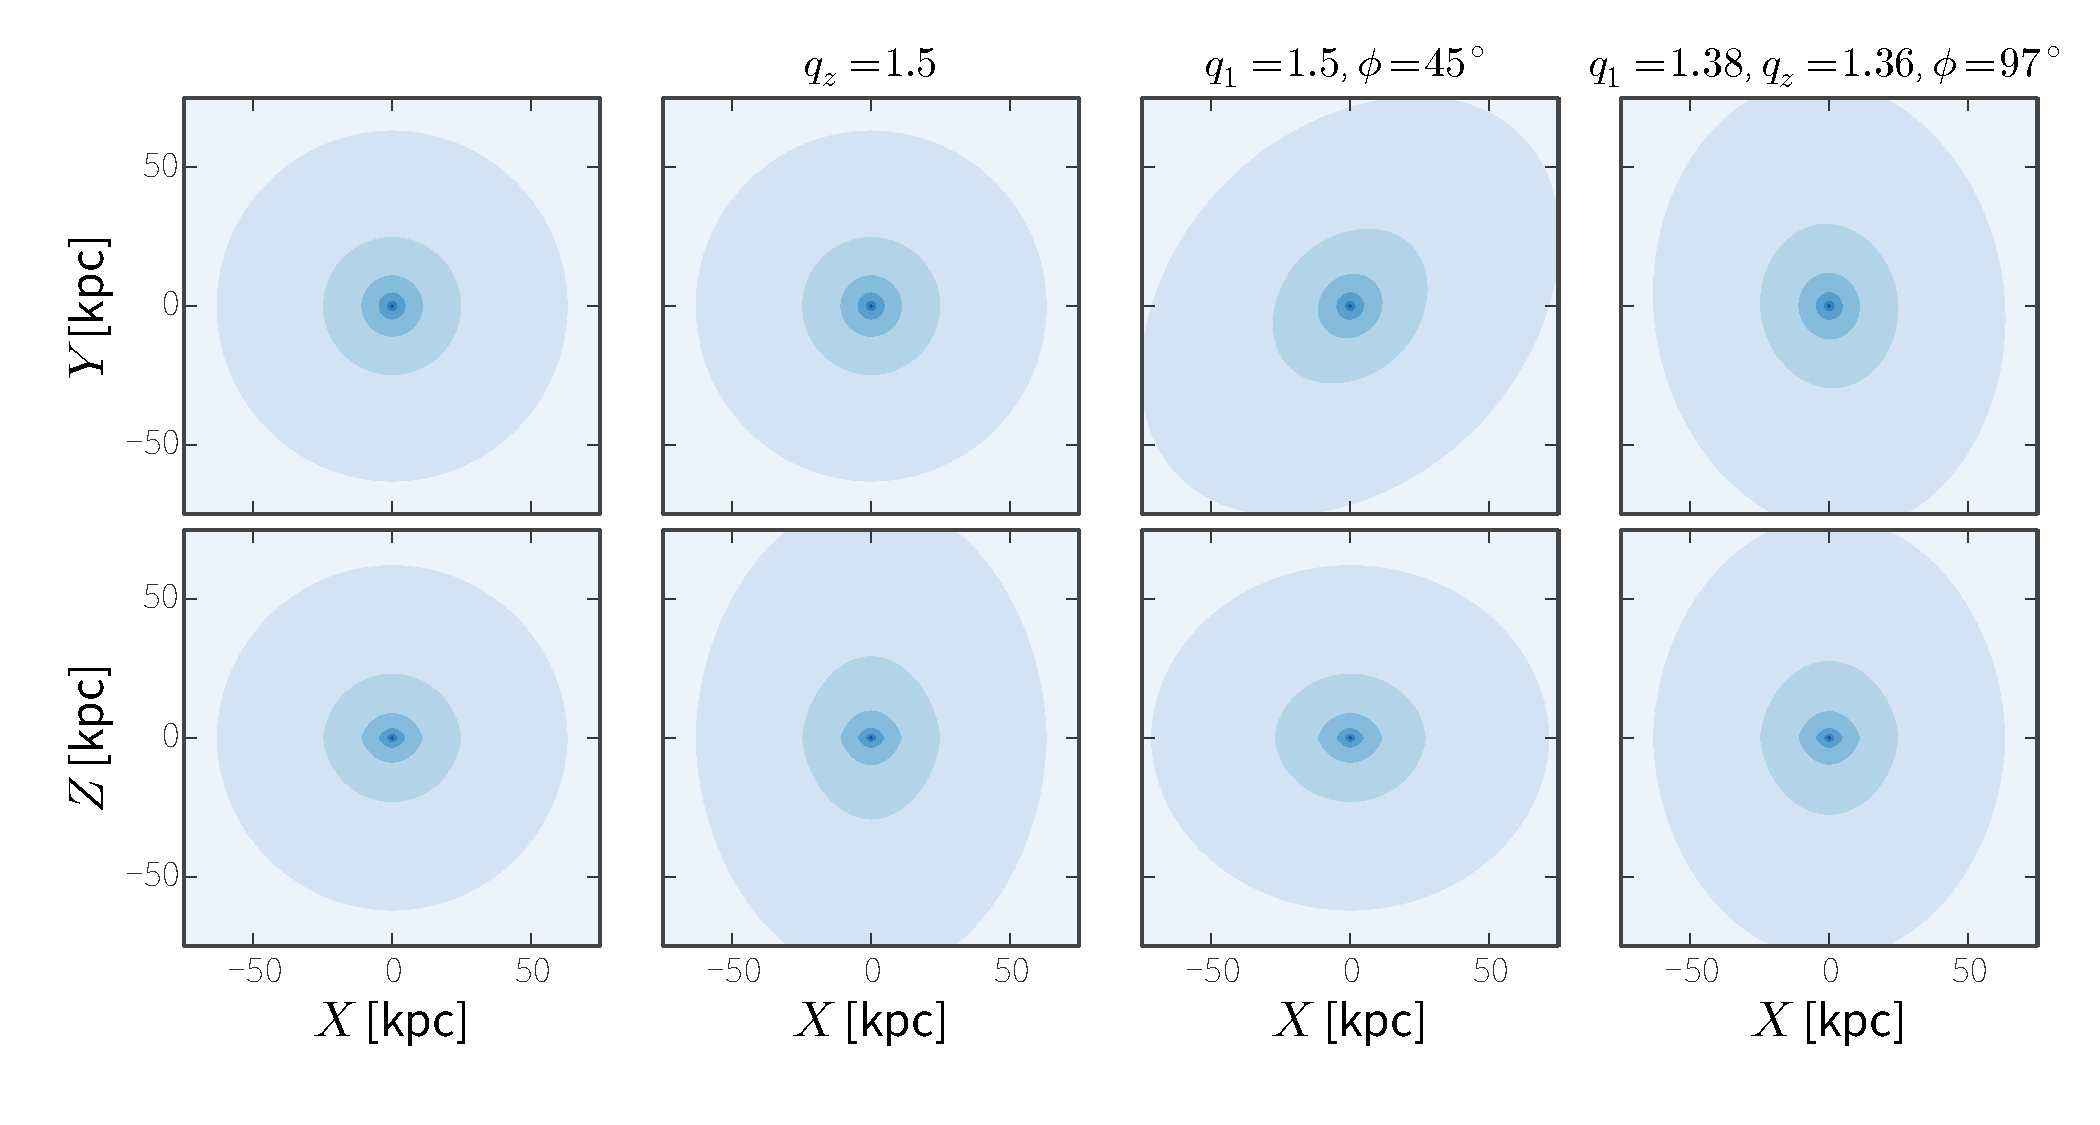
\includegraphics[width=\textwidth]{figures/ch2/potentials.pdf}
\caption{ Equipotential contours for the LM10 potential (Eq.~\ref{eq:lm10}) in
Galactocentric, cartesian coordinates for various halo parameter choices. For
all panels, $\vhalo=121.858~\mathrm{km}/\mathrm{s}$, $\rhalo=12~\mathrm{kpc}$,
and $q_2=1$. Left to right, each column represents a new choice of parameters.
If not specified, other parameters are fixed to $q_1=q_z=1$ and $\phi=0^\circ$
(far left panels). Panels on far right show the best-fit parameter values from
LM10. }\label{fig:ch3-potential}
\end{center}
\end{figure*}

We use this potential not because we think it is a realistic representation of
the Galactic potential, but because successful inference with this potential
demonstrates that it is possible to recover information about non-trivial
potential forms. Figure~\ref{fig:ch3-potential} shows equipotential slices in the
Galactic X-Z plane (Y=0) and Y-Z plane (X=0) for a few choices of  $q_1$,
$q_z$, and $\phi$ while holding all other parameters fixed, as described in the
figure caption. The potential parameters used for the simulations are shown in
the ``Truth'' column of Table~\ref{tbl:params}.

\begin{figure*}[!t]
\begin{center}
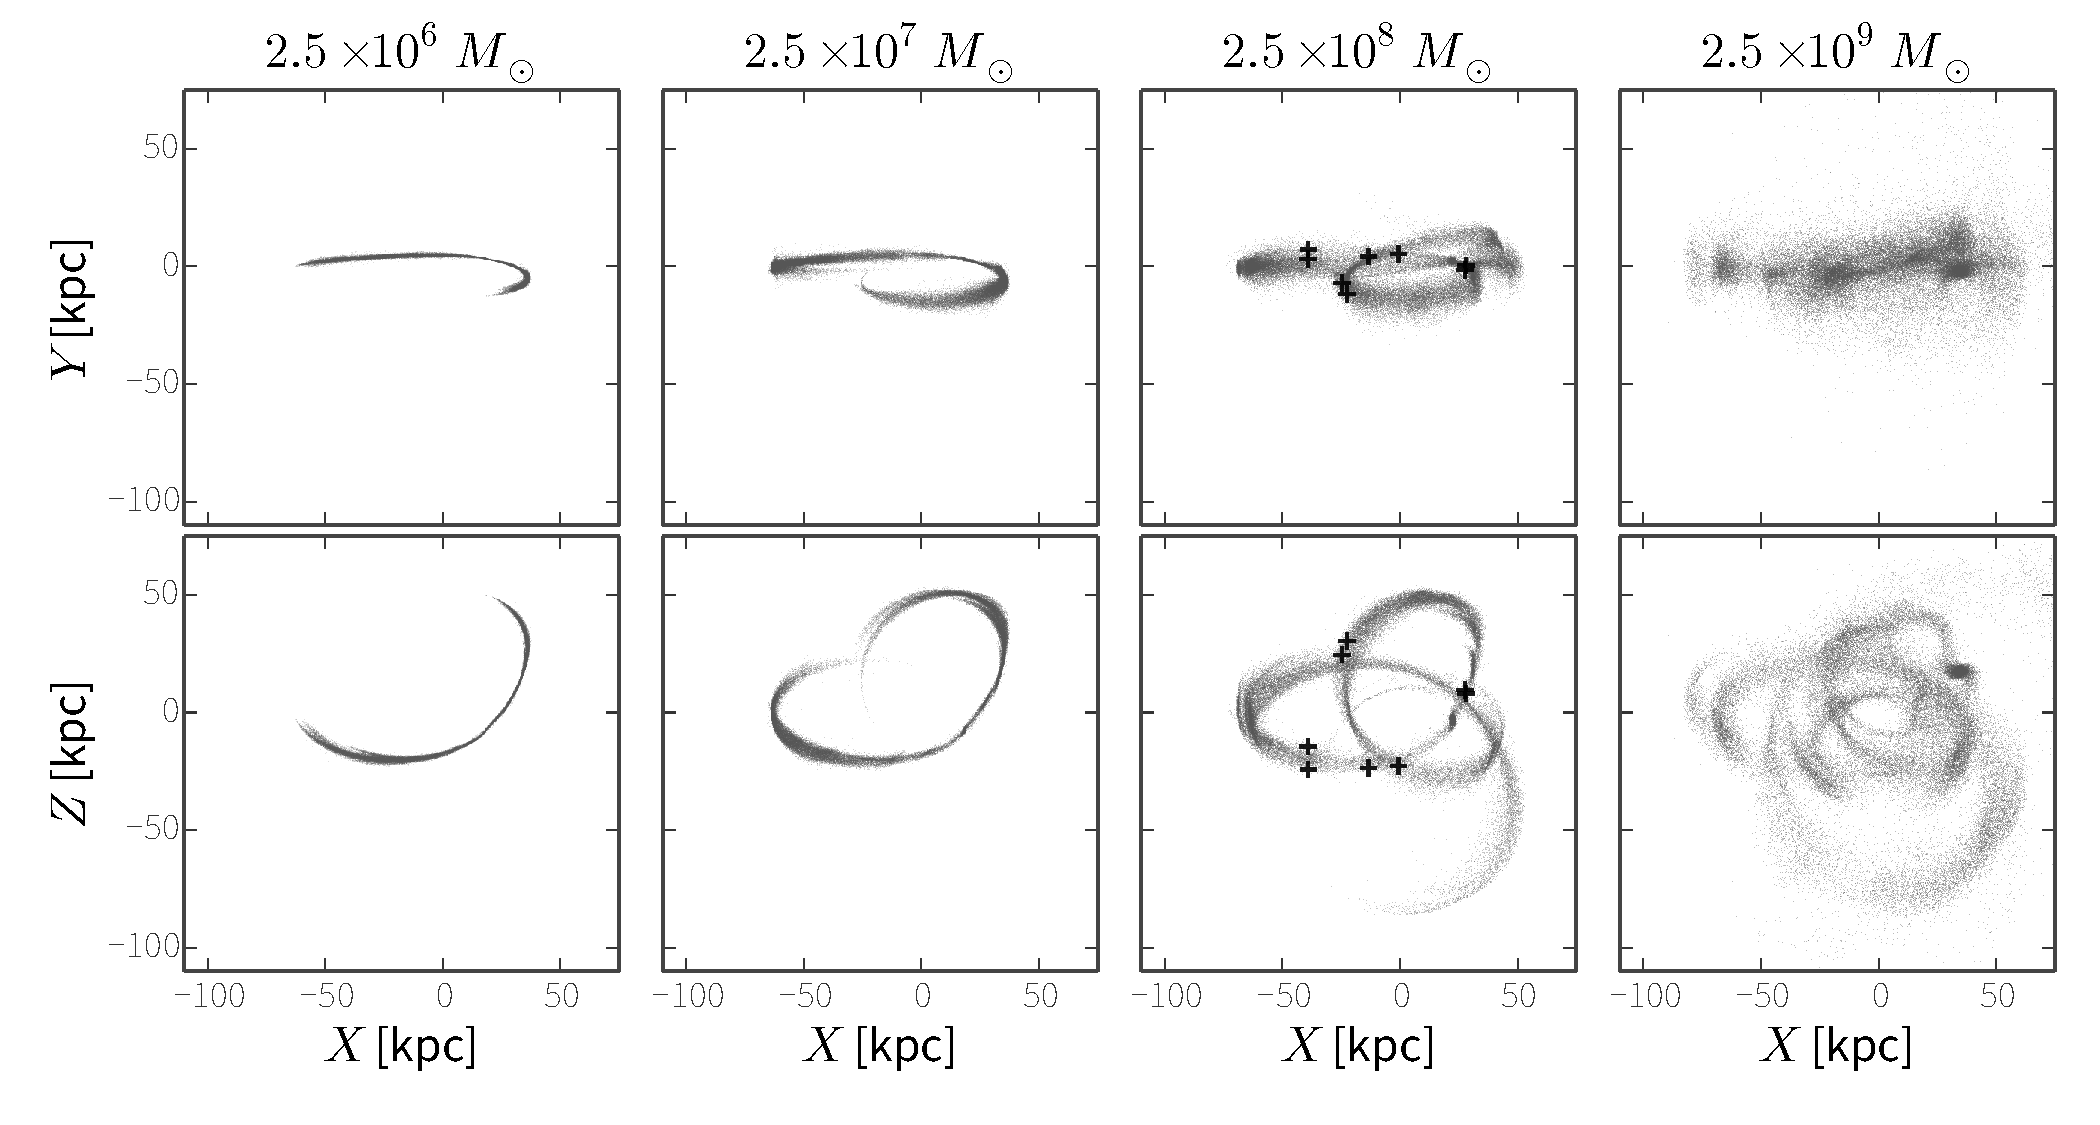
\includegraphics[width=\textwidth]{figures/ch2/simulated_streams.pdf}
\caption{ Particle positions (grey dots) in Galactocentric cartesian coordinates
from the final time-step of four $N$-body simulations (Section~\ref{sec:ch3-sims})
with the same progenitor orbit initial conditions over a range of progenitor
masses (columns). Black crosses indicate eight particles chosen from each mass
simulation and used in the experiments described in
Section~\ref{sec:ch3-experiments}.}\label{fig:sims}
\end{center}
\end{figure*}

\section{Method (\rewinder)}\label{sec:ch3-method}

\rewinder\ integrates stars and the progenitor back from their present-day,
observed positions to the time at which they become unbound from the satellite,
where we evaluate the likelihood for each star. Below we (1) motivate a simple
model for the debris just as it disrupts and (2) present this idea within a
probabilistic framework for incorporating observational uncertainties and
missing data. For a satellite galaxy orbiting within a static host potential,
mass loss is driven by a combination of tidal stripping by the steady tidal
field of the parent system and tidal shocking by the rapidly changing tidal
field as the progenitor system moves through pericenter \citep[e.g.,][]{choi09}.
On a mildly eccentric orbit, the tidal shocking is subdominant to the steady
disruption. The interplay between these two processes as a function of orbital
properties is outside the scope of this \article\ and will be explored in future
work; we focus here on the slow removal of stars by steady tidal forcing.

\subsection{Motivation: tidal debris}\label{sec:ch3-debris}

Consider a point-mass satellite with mass $m$ on a circular orbit with frequency
$\Omega$ around a more massive ``host'' mass $M\gg m$ \citep[the ``restricted
three-body problem''; e.g., \S 8.3][]{binneytremaine}. In a frame rotating with
the orbital frequency of the satellite, the satellite remains fixed and the
static, effective potential around the satellite has (amongst others) two
unstable optima located around galactocentric radii $\sim R \pm r_J$, where $R$
is the orbital radius of the satellite and $r_J$ is the Jacobi or tidal radius
\begin{equation}
	r_J \sim R\left(\frac{m}{3M}\right)^{1/3}.\label{eq:ptmass}
\end{equation}
Particles that would be bound to the satellite in isolation may have enough
(Jacobi) energy to overcome the effective potential barrier at these Lagrange
points (Fig.~8.6 of BT) and thus will be preferentially stripped from the
satellite at these points. For a spherical, extended parent mass distribution
the tidal radius instead scales with the enclosed mass at the instantaneous
orbital radius, $R(t)$, with additional terms that account for the local slope
of the density profile. In general the satellite mass also depends on time. The
tidal radius of the debris then follows
\begin{equation}
	r_{\rm tide}(t) = R(t)\left(\frac{m(t)}{3M_{\rm enc}(R)}\right)^{1/3}\label{eq:tidalradius}
\end{equation}
where $M_{\rm enc}$ is the instantaneous enclosed mass of the parent system
within orbital radius $R$.\footnote{Note that this is the instantaneous orbital
radius, \emph{not} the orbital radius at pericenter.} In general, the Lagrange
points may not be symmetric about the center of the satellite and may deviate
from the tidal radius by factors of order unity.

The bulk velocity of the satellite will be of order $V\sim \sqrt{GM_{\rm
enc}/R}$. If the velocity dispersion of the satellite is $\sigma_v \sim
\sqrt{Gm/r_J}$, then it follows
\begin{equation}
	\sigma_v(t) \sim V\left(\frac{m(t)}{M_{\rm enc}(t)}\right)^{1/3}\label{eq:velscale}.
\end{equation}
\citep[as pointed out in][]{binneytremaine} and hence we expect the debris-star
velocities also to scale with $(m/M_{\rm enc})^{1/3}$. These scalings assume
that the satellite is spherical with isotropic velocities as is reasonable for a
globular cluster or dwarf spheroidal galaxy, but non-random, internal satellite
orbits (e.g., a disk) will break these assumptions.

In a triaxial potential, the orbital plane of the satellite is not fixed but we
still expect there to be \emph{effective} Lagrange points for a spherical
satellite system along the line of centers connecting the origin of the parent
potential to the satellite---that is, we expect the stars to be stripped at
some characteristic distance from the satellite (near the tidal radius) along
the instantaneous position vector of the satellite with some dispersion about
these points. We proceed by defining a coordinate system relative to the
position and velocity of the progenitor, ($\bs{r}_p$,$\bs{v}_p$), rotated into
the instantaneous orbital plane defined by $\bs{L} = \bs{r}_p \times \bs{v}_p$.
The (time-dependent) basis vectors are given by
\begin{align}
	\hat{\bs{x}}_1 &= \frac{\bs{r}_p}{\|\bs{r}_p\|}\label{eq:x1}\\
	\hat{\bs{x}}_2 &= \frac{\bs{L} \times \hat{\bs{x}}_1}{\|\bs{L} \times \hat{\bs{x}}_1\|}\\
	\hat{\bs{x}}_3 &= \hat{\bs{L}} = \frac{\bs{L}}{\|\bs{L}\|} = \frac{\bs{r}_p \times \bs{v}_p}{\|\bs{r}_p \times \bs{v}_p\|}\label{eq:x3}.
\end{align}
\begin{figure}[t!]
\begin{center}
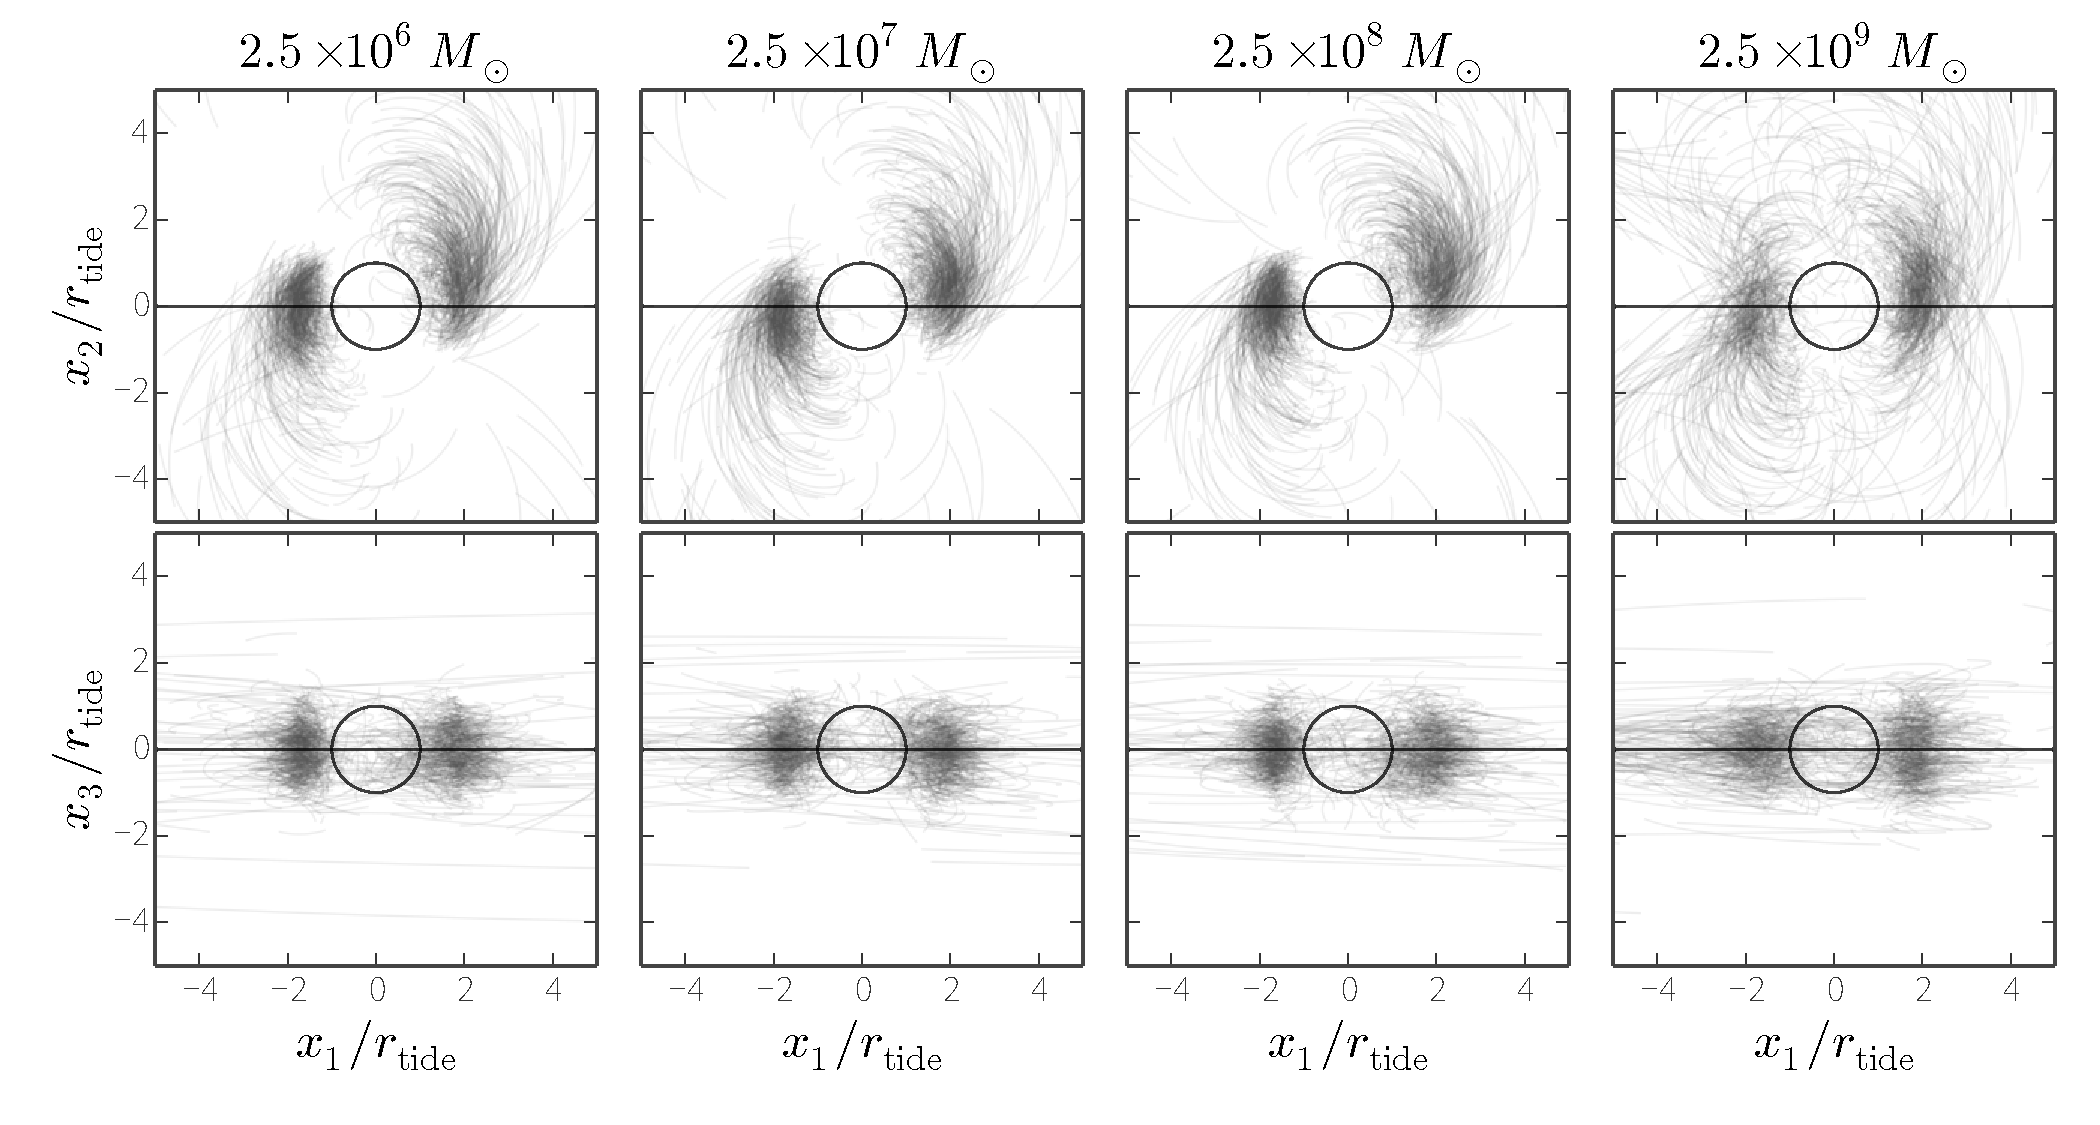
\includegraphics[width=0.9\textwidth]{figures/ch2/Lpts_r.pdf}
\caption{ Orbits of 2000 randomly-drawn, disrupted particles projected into the
instantaneous orbital plane coordinates (Eqs.~\ref{eq:x1}-\ref{eq:x3}),
normalized by the tidal radius (Eq.~\ref{eq:tidalradius}), and only shown within
half a satellite crossing time around $t=\tub$ for each of the four progenitor
masses. The orbits were integrated backwards from their present-day positions
(final time step of the $N$-body simulations) as test particles without the
potential of the progenitor. Horizontal black line shows $x_2=0$ (top panels)
and $x_3=0$ (bottom panels), and the unit circle (black circle) illustrates the
classical disruption radius in these coordinates. }\label{fig:lpts_r}
\end{center}
\end{figure}
Figure~\ref{fig:lpts_r} shows sections of particle orbits (for particles that
are stripped) from the $N$-body simulations described above, projected into this
coordinate system. The positions are normalized by the instantaneous tidal
radius (Eq.~\ref{eq:tidalradius}) and velocities are normalized by the
instantaneous velocity scale (Eq.~\ref{eq:velscale}). Sections of the orbits
symmetric around their unbinding times, $\tub$, are shown for each of the four
progenitor masses. In these coordinates, the classical Lagrange points would be
located at $x_1\approx\pm\rtide,x_2=0,x_3=0$ (illustrated by the intersection of
the black unit circles and horizontal lines in Figure~\ref{fig:lpts_r}). Though
not exactly centered on the point-mass Lagrange points derived for a circular
orbit, the location of and dispersion about the effective Lagrange points in
these scaled coordinates remain remarkably consistent across the range of
progenitor masses explored. Figure~\ref{fig:lpts_v} shows the velocity orbits of
each star also projected into these coordinates and normalized. The dispersion
in velocity is well-normalized by the velocity scale of Eq.~\ref{eq:velscale},
though it is clear that the velocity dispersion along $\hat{x}_1$, the radial
vector to the satellite position, is larger than that in other dimensions,
possibly because of mild tidal shocking.
\begin{figure}[t!]
\begin{center}
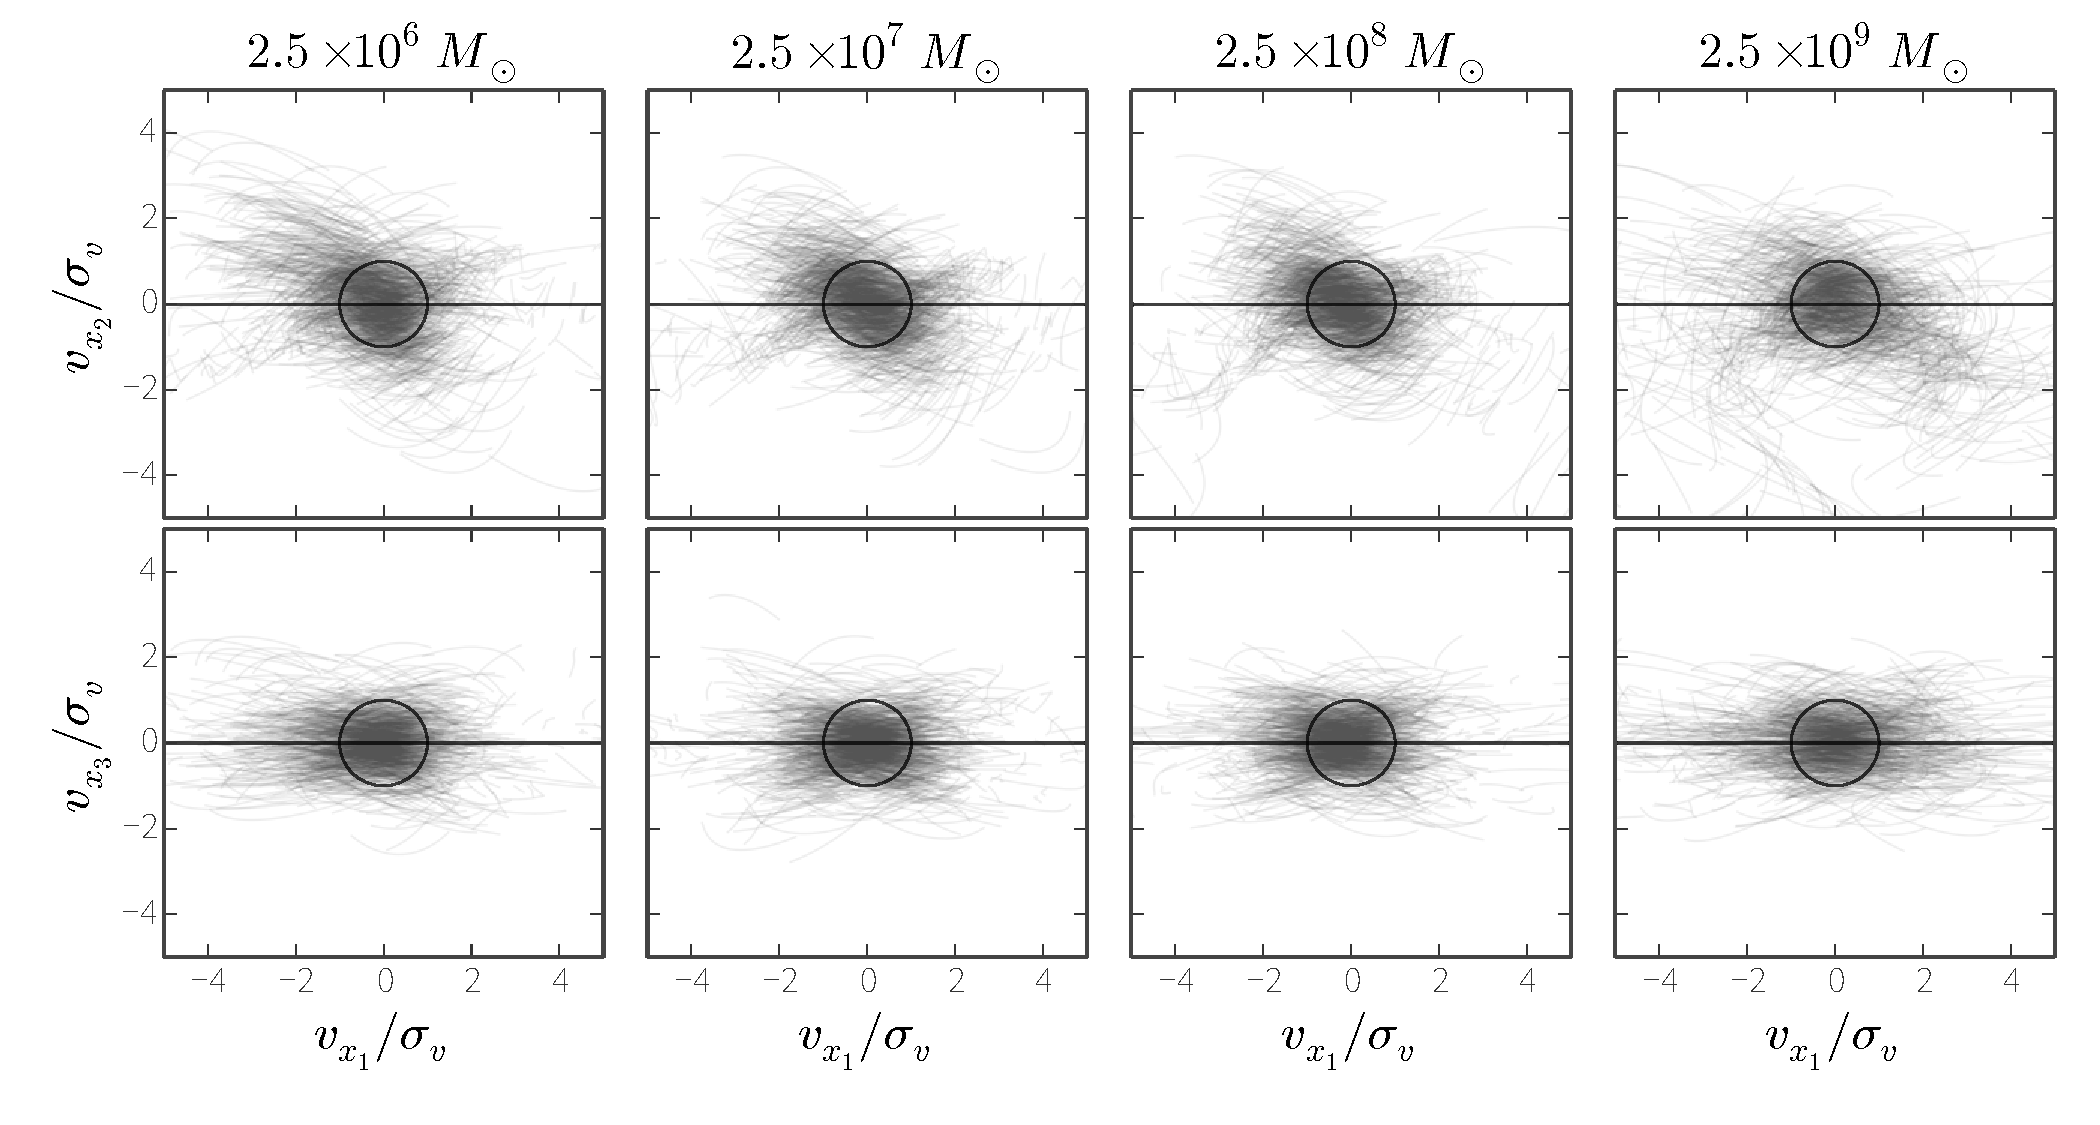
\includegraphics[width=0.9\textwidth]{figures/ch2/Lpts_v.pdf}
\caption{ Same as Figure~\ref{fig:lpts_r} but for particle velocities normalized by the velocity scale (Eq.~\ref{eq:velscale}). }\label{fig:lpts_v}
\end{center}
\end{figure}

We conclude that even on a non-circular orbit in a complex potential, the
dispersion---in position and velocity---of tidally stripped debris as it
comes unbound from the satellite scales with the mass ratio $(m / M_{\rm
enc})^{1/3}$. This motivates a model for tidal debris in which each star was
``released'' at the instantaneous, effective Lagrange point at its unbinding
time, $\tub$, with a dispersion in position and velocity, all of which depend
only on the mass and orbit of the progenitor and the parent potential. We
present this model in detail below.%\clearpage

\subsection{Probabilistic model}
Suppose we observe the 6D position of a star, $\D = (l,b,d,\mu_l,\mu_b,v_r)$, in
heliocentric coordinates---e.g., the measured position on the sky, ($l$, $b$);
distance, $d$; proper motions, ($\mu_l$, $\mu_b$); and line-of-sight velocity,
$v_r$---and have determined through some other means that this star was once
part of a progenitor system (e.g., satellite galaxy) with mass $m(t)$ that is
disrupting and forming a cold debris structure in the potential, $\Phi$, of the
parent galaxy (e.g., the Milky Way). We assume that the mass of the parent
system enclosed within the pericenter of the orbit of the satellite, $M_{\rm
enc}(R_{\rm peri})$, is much larger than the initial mass of the satellite,
$M_{\rm enc}(R_{\rm peri})\gg m(t=0)$. The present position of the progenitor is
observed to be at heliocentric position $\D_\sat$ (where any subscript $\sat$
refers to the progenitor). In general, the data for the star and progenitor will
have significant uncertainties or missing dimensions at distances typical to the
Galactic halo, thus we define $\W$ and $\W_\sat$ as the true 6D, heliocentric
positions of the star and progenitor and will include these in our model. Since
we include these positions as parameters, this method will work even when the
star has missing dimensions or the progenitor location is unknown \citep[as in
the Orphan stream,][]{belokurov07}.

To model the true, 6D, present-day position of the star, $\W$, we first
transform to cartesian, Galactocentric coordinates where ($\bs{r}_0,\bs{v}_0$)
and ($\bs{r}_{\sat,0},\bs{v}_{\sat,0}$) are the position and velocity of the
star and progenitor today. The star is taken as having been sampled at $t=\tub$
(the unbinding time) from an isotropic Gaussian centered on one of the effective
Lagrange points in position, and an isotropic Gaussian centered on the origin in
velocity. The present-day phase-space position is the result of integrating this
sample forward from $\tub$ in the parent potential, $\Phi$, whose form is
parametrized by the vector $\bs{\Theta}_\Phi$. We assume that once the star
becomes ``unbound'' from the satellite the potential of the satellite can be
ignored,\footnote{This assumption breaks down for sufficiently large-mass
progenitors with total mass somewhere between $\sim10^8-10^9~\msun$.} and thus
we treat the star as a test particle.

The satellite mass enters this prescription through the tidal radius; a changing
satellite mass will skew the positions of the effective Lagrange points and
velocity scale. We allow for mass-loss by incorporating the initial satellite
mass, $m_0$, and a constant mass-loss term, $\dot{m}$ into the model: $m(t) =
m_0 - \dot{m}t$. We assume constant mass-loss as an example of a simple,
monotonically decreasing function, but this an arbitrary choice. We don�t expect
this assumption to have a large effect on our conclusions as the mass only
enters the model through the tidal radius as $m^{1/3}$: even if we ignored
mass-loss entirely, the progenitor and orbit considered here has lost 75\% of
its mass by the end of the simulation corresponding to a factor of just
$\sim$1.6 difference in tidal radius. In principle, with more data, the
mass-loss history could be inferred self-consistently by the model, but we leave
this exercise for future work.

Finally, we add two additional parameters: a constant, global factor,
$\Loffset$, that scales the position of the effective Lagrange points relative
to the classical tidal radius, and a binary parameter $\tailbit$ (one for each
star), that is either $-1$ or $+1$ depending on whether the star is in the
leading or trailing tail. To compress notation, we pack all progenitor
parameters into the vector $\bs{\Theta}_\sat = (\W_\sat, m_0, \dot{m},
\Loffset)$. The likelihood for this model is:
\begin{align}
	p(\W \given \bs{\Theta}_\sat, \bs{\Theta}_\Phi, \tailbit, \tub) &= p(\bs{r}_0,\bs{v}_0, \given \bs{\Theta}_\sat, \bs{\Theta}_\Phi, \tailbit, \tub)\,\left\vert\J\right\vert\label{eq:starlike}\\
	p(\bs{r}_0,\bs{v}_0, \given \bs{\Theta}_\sat, \bs{\Theta}_\Phi,\tailbit,\tub) &= \left[\mathcal{N}(\bs{r} \given \bs{\Theta}_\sat, \tailbit)\,\mathcal{N}(\bs{v} \given \bs{\Theta}_\sat)\right]_{\tub}
\end{align}
where $\mathcal{N}$ represents the normal distribution, $\rtide$ is given by
Eq.~\ref{eq:tidalradius}, and $\sigma_v$ by Eq.~\ref{eq:velscale} and the
positions and velocities ($\bs{r},\bs{v}, \bs{r}_{\sat},\bs{v}_{\sat}$) are
evaluated at the unbinding time, $\tub$, by integrating the orbits backwards
from ($\bs{r}_0,\bs{v}_0, \bs{r}_{\sat,0},\bs{v}_{\sat,0}$).
$\left\vert\J\right\vert = \left\vert\frac{\partial(x,y,z,v_x,v_y,v_z)}{\partial
(l,b,d,\mu_l,\mu_b,v_r)}\right\vert$ is the absolute value of the determinant of
the Jacobian that defines the transformation from heliocentric, spherical to
Galactocentric, cartesian coordinates. We then marginalize the likelihood over
all possible unbinding times, assuming a uniform prior of unbinding times over
the entire interaction time:
\begin{align}
	p(\W \given \bs{\Theta}_\sat, \bs{\Theta}_\Phi, \tailbit) &= \int^{t_{\rm int}}_0 p(\W \given \bs{\Theta}_\sat, \bs{\Theta}_\Phi, \tailbit, \tub)\,p(\tub)\,d\tub
\end{align}
where the interaction time is taken to be $t_{\rm int}=6$~Gyr, the total
duration of the simulations of Section~\ref{sec:ch3-sims}.

The likelihood above is evaluated for each star at all time-steps of the
simulation during the marginalization with a uniform prior over all possible
unbinding times. We chose this approach because the phase-space position (and
hence time) at which a star becomes unbound from a satellite can only be
strictly defined for the case of a spherical satellite orbiting on a circular
orbit in a spherical potential. Various authors have chosen to measure mass loss
in simulations of satellite disruption on eccentric orbits in non-spherical
potentials by either looking at the kinetic energy of the particles relative to
the satellite's potential energy \citep{johnston95} or looking at the point at
which a star crosses the instantaneous tidal radius \citep{kuepper12}. Neither
choice is strictly valid and both have been found useful for representing the
mass-loss process. Hence we make the simplest choice of using Gaussians to
characterize the phase-space distribution of debris as it makes the transition
between being bound and unbound. We find that changing this distribution to a
log-normal distribution does not affect our conclusions.

We assume that the observational uncertainties are Gaussian in heliocentric,
spherical coordinates, such that
\begin{align}
	p(\D \given \W) &= \mathcal{N}(\D \given \W, \bSigma)\label{eq:obsstar}\\
	p(\D_\sat \given \W_\sat) &= \mathcal{N}(\D_\sat \given \W_\sat, \bSigma_\sat)\label{eq:obsprog}
\end{align}
where the covariance matrices $\bSigma$ and $\bSigma_\sat$ specify the
observational uncertainties on the observed 6D position of the star and
progenitor, respectively.

For a single star, the evaluation of the likelihood works as follows: given
observed, present-day coordinates for the star and progenitor ($\D,\D_\sat$),
potential parameter values ($\bs{\Theta}_\Phi$), and nuisance parameter values
($\Loffset,\tailbit$),
\begin{enumerate}
	\item transform star and progenitor positions in heliocentric coordinates to Galactocentric, cartesian coordinates;
	\item integrate star and progenitor orbits backwards as test particles in the potential given by $\bs{\Theta}_\Phi$ for the total interaction time, $t_{\rm int}$ (in this case, $\sim$$6$~Gyr);
	\item transform the particle position to the relative, normalized coordinates defined in Section~\ref{sec:ch3-debris};
	\item compute the likelihood given by Equation~\ref{eq:starlike} at each time-step of the integration and marginalize over the unbinding time, $\tub$.
\end{enumerate}

Assuming each star is an independent tracer, the full likelihood for many stars
is then just the product of the individual likelihoods:
% multline for 2 column format
%\begin{multline}
%	p(\{\D^{(i)}\}, \D_\sat \given \{\bs{\Theta}^{(i)}\}, \bs{\Theta}_\sat, \bs{\Theta}_\Phi ) = \\
%		p(\D_\sat \given \W_\sat) \, \prod_i \, p(\D^{(i)} \given \W^{(i)}) \,
%			p(\W^{(i)} \given \bs{\Theta}_\sat, \bs{\Theta}_\Phi, \tailbit^{(i)})
%\end{multline}
\begin{equation}
	p(\{\D^{(i)}\}, \D_\sat \given \{\bs{\Theta}^{(i)}\}, \bs{\Theta}_\sat, \bs{\Theta}_\Phi ) =
		p(\D_\sat \given \W_\sat) \, \prod_i \, p(\D^{(i)} \given \W^{(i)}) \,
			p(\W^{(i)} \given \bs{\Theta}_\sat, \bs{\Theta}_\Phi, \tailbit^{(i)})
\end{equation}
where $\bs{\Theta}^{(i)} = (\W^{(i)}, \tailbit^{(i)})$. All parameters are summarized in Table~\ref{tbl:params}.

\section{Experiments} \label{sec:ch3-experiments}
In what follows, we use \rewinder\ to model ``observations'' of a small sample
of stars from one of the $N$-body simulations described in Section~\ref{sec:ch3-sims}.
We consider this a strong test of the method because the data are generated with
$N$-body simulations that do not resemble the likelihood function presented above.
For all tests in this \article, we use the same functional form for the potential
as used in the simulations (Equation~\ref{eq:lm10}). When recovering the
potential, we hold fixed the disk and spheroid parameters (see
Table~\ref{tbl:params}), along with one of the halo parameters: the scale
radius, $\rhalo$. The priors on the remaining halo parameters are taken to be
uniform over a conservative domain of realistic values: for $\vhalo$,
100-200~km/s corresponds to a range in solar circular velocities from
$\sim$210-250 km/s (holding other parameters fixed); the range in axis ratios
allow for prolate, oblate, and generic triaxiality; and $\phi$ is restricted to
$\pm45^\circ$ around the true simulation value, $\phi = 97^\circ$.

For all experiments below, we use a Markov Chain Monte Carlo (MCMC) algorithm to
sample from the posterior probability distribution given by our model. Standard
MCMC algorithms (e.g., Metropolis-Hastings) update a single chain while
exploring parameter space. We instead use an affine-invariant ``ensemble''
sampler \citep{goodman10} that at each step in parameter space, updates the
positions of many ``walkers'' (the ensemble). This algorithm is implemented in
the \python\ programming language \citep{foremanmackey13} and runs
naturally in a parallelized environment such as the message passing interface
(MPI). In each experiment we run the walkers for a large number of steps from
starting positions described below, then throw away these samples and take the
positions from the final step of this ``burn-in'' phase as a starting point for
the samples used for inference. We compute the autocorrelation time, $t_{\rm
acor}$, for each sampled parameter (using\project{ACOR}\footnote{\url{http://www
.math.nyu.edu/faculty/goodman/software/acor/}}$^{,}$\footnote{\url{https://githu
b.com/dfm/acor}}) and thin the chains by taking every $\mathrm{max}(t_{\rm
acor})$ sample to ensure the samples are close to independent. The
autocorrelation time measures the number of steps required to produce
independent samples from the posterior probability distribution: a shorter
autocorrelation time means that fewer steps (and therefore fewer likelihood
evaluations) are required to produce close to independent samples from the
posterior.

\begin{table*}[ht]
\begin{center}
	\begin{tabular}{l c c l} \toprule
		\multicolumn{4}{l}{{\bf \emph{Milky Way parameters} ($\bs{\Theta}_\Phi$)}} \\
		\toprule
		Component & Parameter & Truth & Prior \\\toprule
		disk & $M_{\rm disk}$ & $1.0\times10^{11}\,\msun$ & fixed \\
		& $a$ & 6.5 kpc & fixed\\
		& $b$ & 0.26 kpc & fixed\\
		\midrule
		spheroid & $M_{\rm spher}$ & $3.4\times10^{10}\,\msun$ & fixed\\
		& $c$ & 0.7 kpc & fixed\\
		\midrule
		halo & $\vhalo$ & 121.858 & $\mathcal{U}(100,200)$ km/s \\
		& $q_1$ & 1.38 & $\mathcal{U}(1,2)$\\
		& $q_2$ & 1.0 & fixed\\
		& $q_z$ & 1.36 & $\mathcal{U}(1,2)$\\
		& $\phi$ & 97 & $\mathcal{U}(52,142)$ deg\\
		& $\rhalo$ & 12 kpc & $\mathcal{U}(8, 50)$ kpc\\
		\toprule
		\multicolumn{4}{l}{{\bf \emph{Progenitor parameters} ($\bs{\Theta}_\sat$)}} \\
		\toprule
		position & $\bs{r}_{\sat,0}$ & -- & $\|\bs{r}_{\sat,0}\|\sim\mathcal{U}(0,200)$~kpc \\
		velocity & $\bs{v}_{\sat,0}$ & -- & $\|\bs{v}_{\sat,0}\|\sim\mathcal{U}(0,500)$~km/s\\
		Lagrange pt. offset & $\alpha$ & -- & $\mathcal{U}(0.5, 2.5)$\\
		initial mass & $m_0$ & $2.5\times10^8\,\msun$ & fixed\\
		mass loss & $\dot{m}$ & -- & $3.2\times10^4\,\msun$/Myr (fixed)\\
		\toprule
		\multicolumn{4}{l}{{\bf \emph{Star parameters} ($\bs{\Theta}^{(i)}$)}} \\
		\toprule
		position & $\bs{r}_0$ & -- & $\|\bs{r}_0\|\sim\mathcal{U}(0,200)$~kpc \\
		velocity & $\bs{v}_0$ & -- & $\|\bs{v}_0\|\sim\mathcal{U}(0,500)$~km/s\\
		tail assignment & $\beta$ & -- & $\pm1$~equally likely (fixed at truth)\\
		\bottomrule
		\end{tabular}
    \caption{Parameter values used in the experiments of
    Section~\ref{sec:ch3-experiments}. $\mathcal{N}$ is the normal (Gaussian)
    distribution, and $\mathcal{U}$ the uniform distribution. There are 11
    parameters for the Milky Way potential, but only the halo parameters are
    left free to vary; some parameters are fixed (denoted by ``(fixed)'') at the
    true values used in the $N$-body simulations that generated the fake test
    data. The progenitor has nine parameters---the position, $\bs{r}_{\rm p}$,
    and velocity, $\bs{v}_{\rm p}$, vectors each contain three components---but
    only five are left free to vary. The sky coordinates (e.g., Galactic $l$,
    $b$) are assumed to be known with negligible uncertainty. Each star has
    eight associated parameters, five of which are allowed to vary. Sky
    coordinates are fixed, along with the tail assignment (whether the star
    belongs to the leading or trailing tail). For inference with eight stars,
    there are $4+5+8\times4=41$ free parameters. \label{tbl:params}}
\end{center}
\end{table*}

\subsection{Data with negligible uncertainties}\label{sec:ch3-exp1}

We test \rewinder\ using only eight stars (particles)---four from the leading
tail, and four from the trailing tail---randomly sampled from the
$2.5\times10^8\,\msun$ simulation (Section~\ref{sec:ch3-sims}), assuming the
observed 6D positions for both the stars and the progenitor have negligible
uncertainties. The stars were required to have been stripped after the first
pericentric passage and have a present-day distance within $40$ kpc of the Sun.
Figure~\ref{fig:sims} (second column from right) shows the randomly chosen stars
(black crosses) in Galactic coordinates, over-plotted on all other simulated
particles (grey points).

We leave the potential parameters ($q_1,q_z,\phi,\vhalo,\rhalo$) free to vary,
along with the Lagrange point offset, $\Loffset$, and initialize an ensemble of
64 MCMC walkers by sampling from the priors summarized in
Table~\ref{tbl:params}. We run the walkers for 5000 steps to burn-in, then
restart the sampler starting from the final position of the burn-in phase and
run for another 10000 inference steps. Figure~\ref{fig:trace} shows the walker
positions over the 10000 inference steps for each of the parameters. The
autocorrelation time for each parameter is displayed on its corresponding panel.
Figure~\ref{fig:exp1_posterior} shows projections of the posterior probability
distribution for the parameters; with perfect data, the uncertainties on the
potential parameters are all $<1\%$.

\begin{figure}[p]
\begin{center}
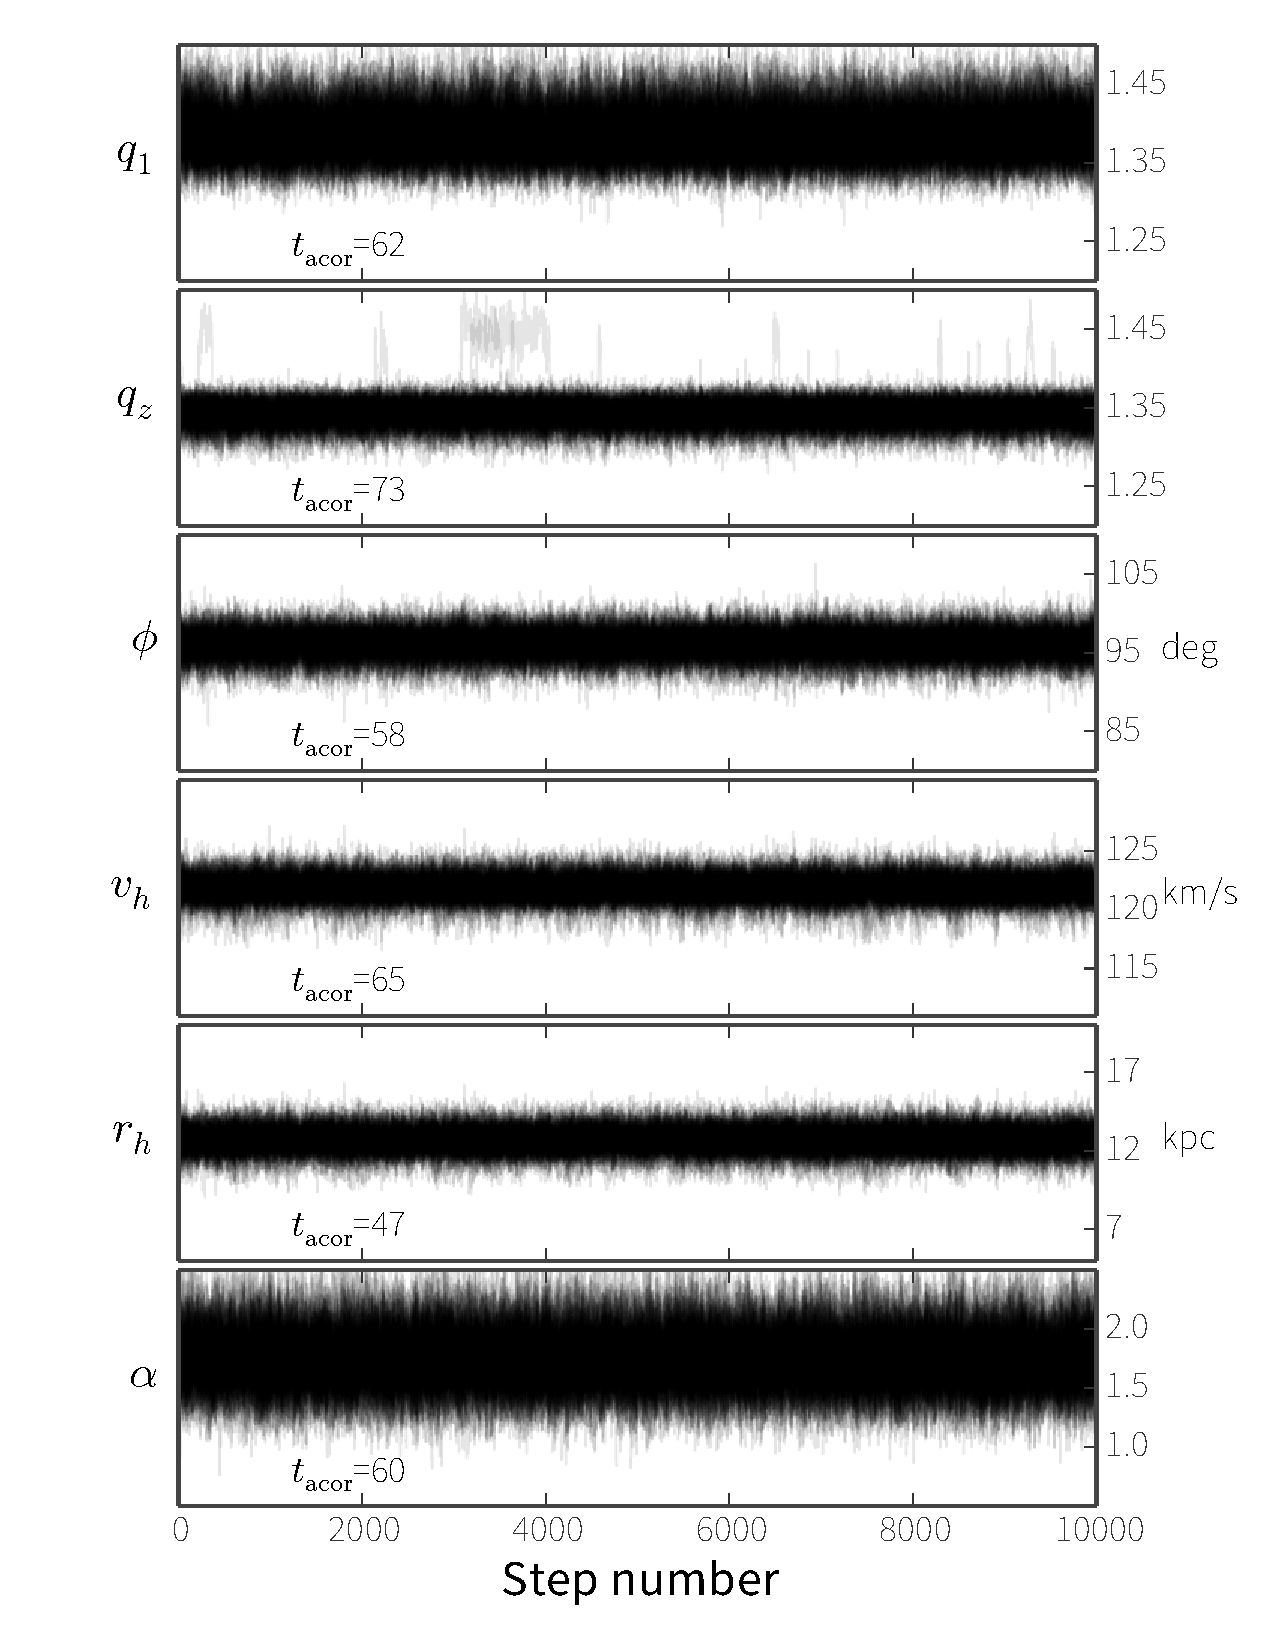
\includegraphics[width=0.7\textwidth]{figures/ch2/mcmc_trace.pdf}
\caption{ Positions of all 64 MCMC walkers (see Section~\ref{sec:ch3-experiments})
for each parameter at each step of the inference (black lines). The MCMC chains
do not display any bulk movement or stray walkers, implying, by eye, that the
chains have converged. We also compute the autocorrelation functions for each
parameter and find that, for this experiment, the autocorrelation times are
short (as shown on each panel in this figure). Projections of the binned samples
(posterior densities) are shown in Figure~\ref{fig:exp1_posterior}.
}\label{fig:trace}
\end{center}
\end{figure}

\begin{figure*}[!h]
\begin{center}
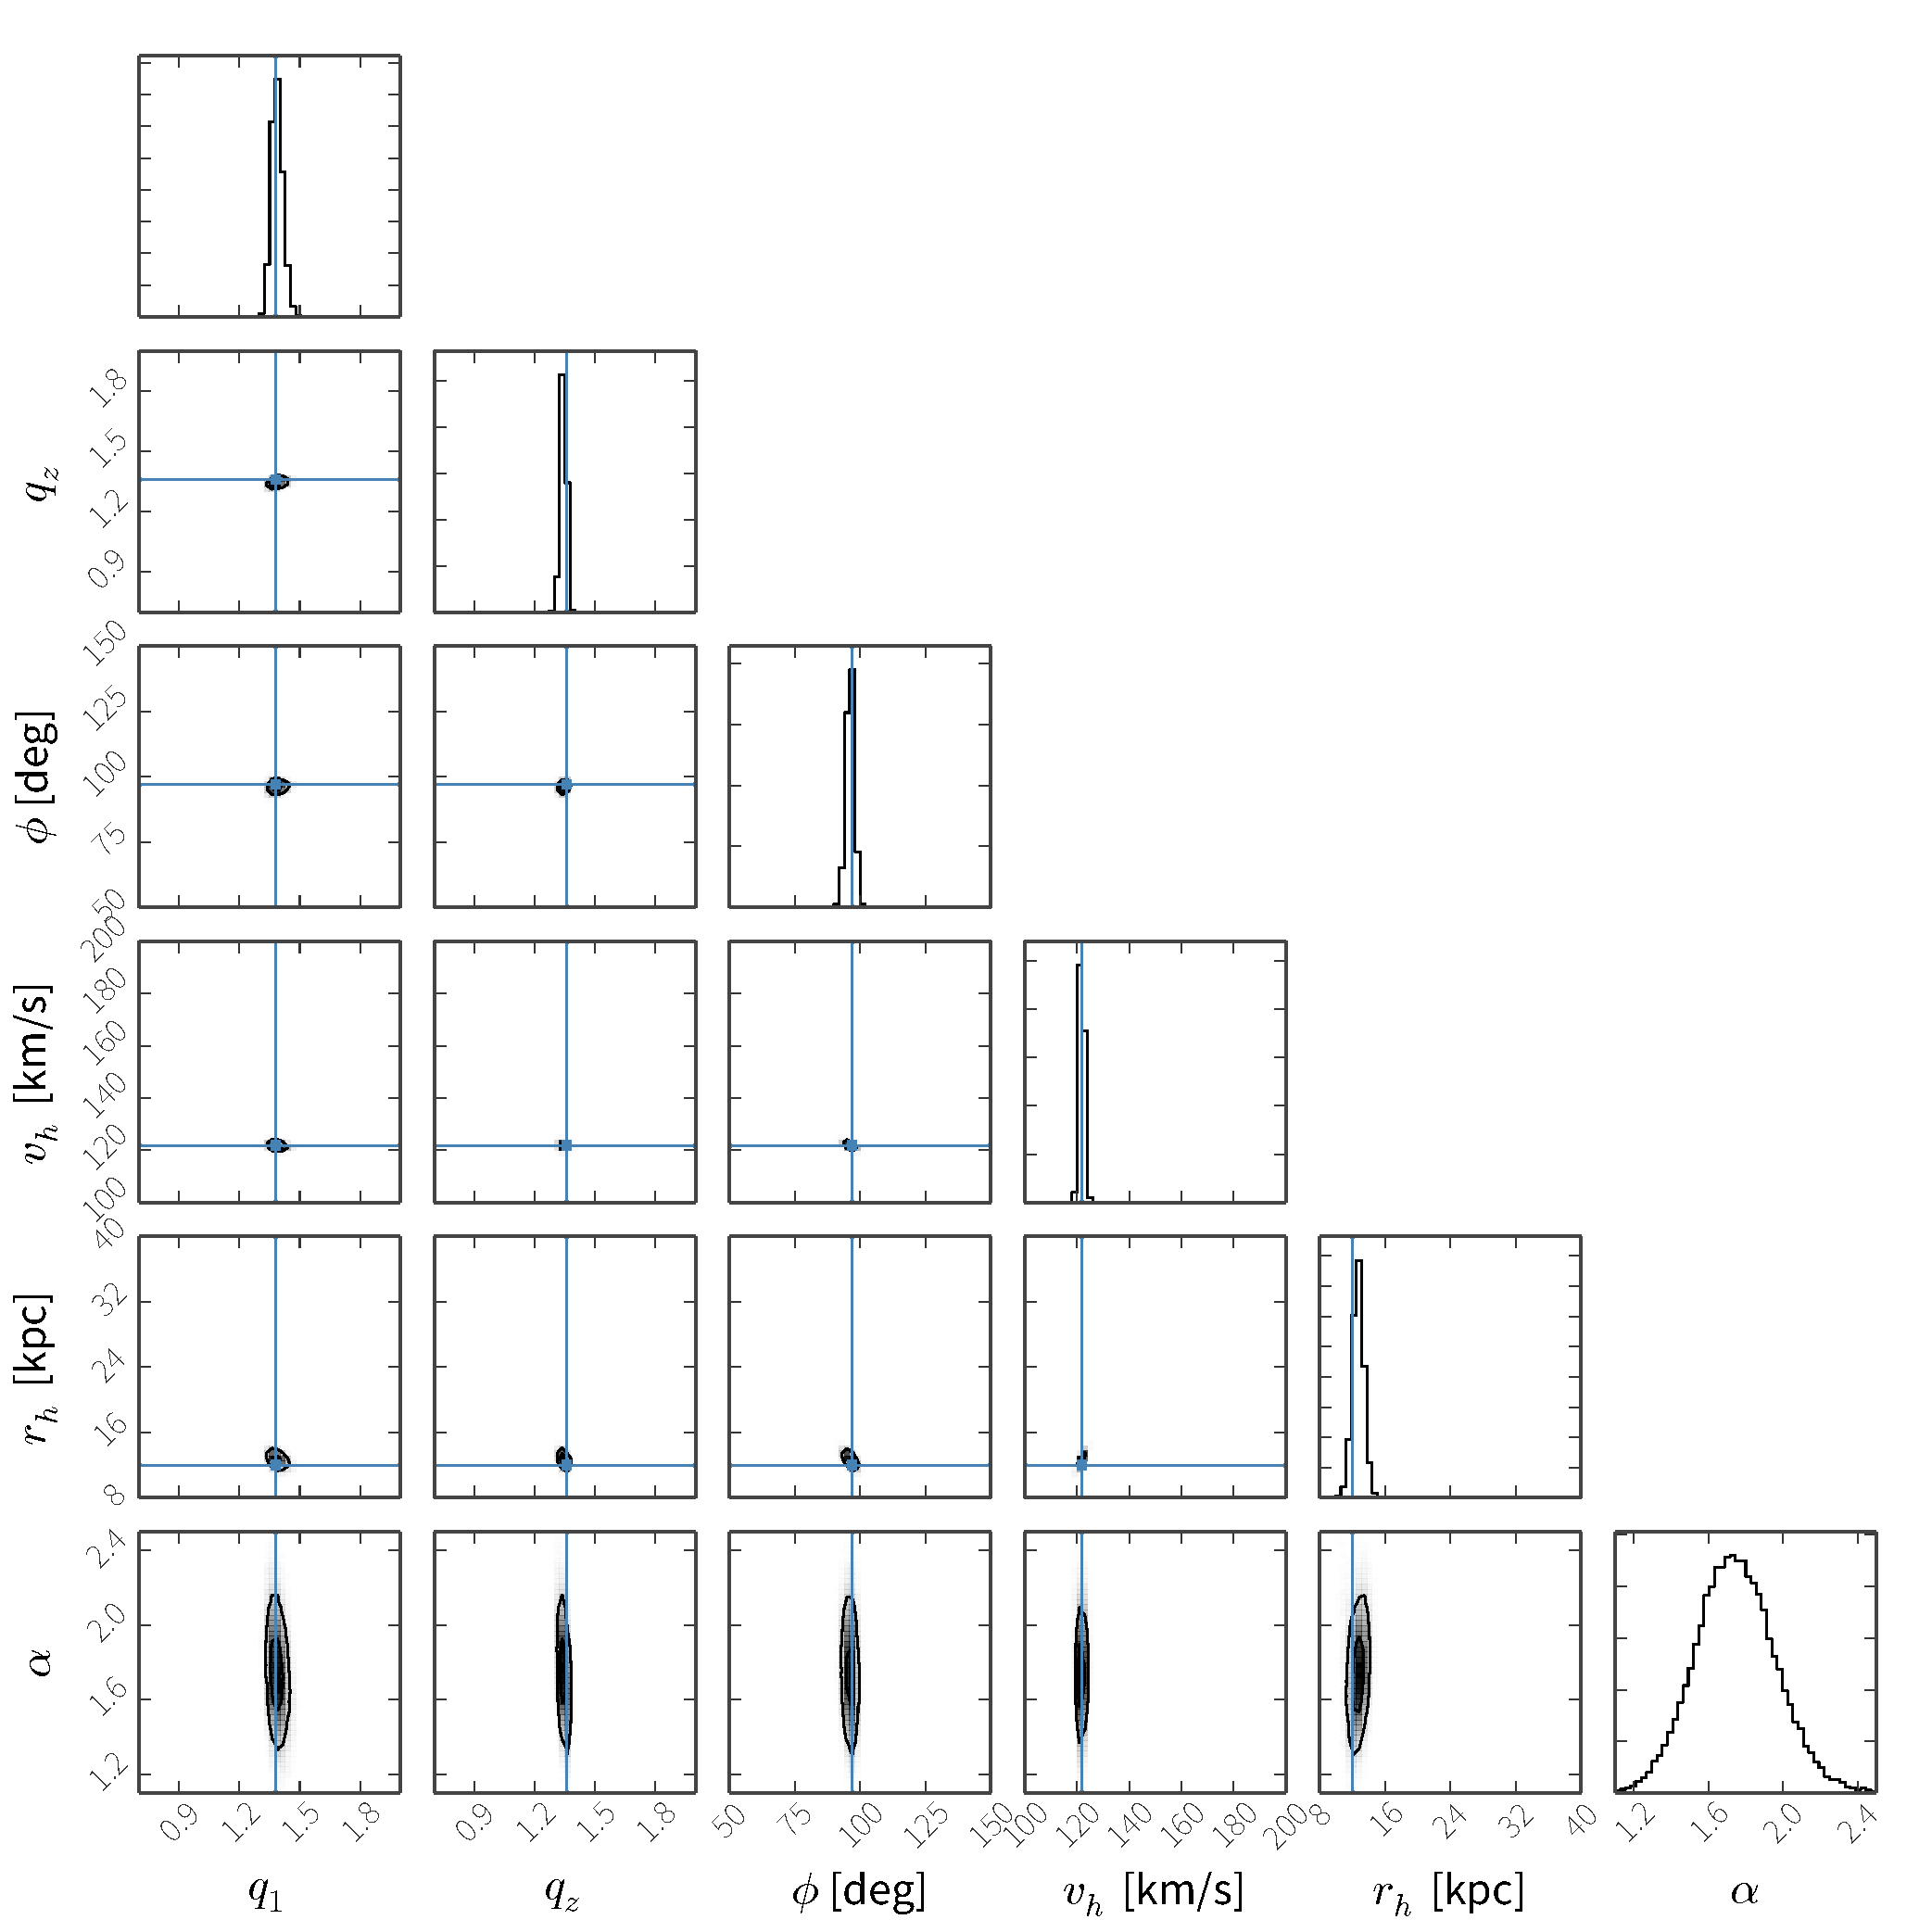
\includegraphics[width=\textwidth]{figures/ch2/exp1_posterior.pdf}
\caption{ Projections of the posterior probability distribution over the five
potential parameters (\potp) and Lagrange point offset ($\alpha$) assuming
negligible uncertainties on the observed phase-space coordinates of eight stars
and the progenitor, visualized as two-dimensional histograms of MCMC samples.
Solid contours (black lines) show approximately 1$\sigma$ and 2$\sigma$ levels
of the distribution. Vertical and horizontal lines (blue) show the true, input
values for the potential parameters used in the $N$-body simulations. For the
potential parameters, the axis ranges are chosen to be the same for this and the
potential posterior plots to follow. }\label{fig:exp1_posterior}
\end{center}
\end{figure*}

\subsection{Data with near-future uncertainties}\label{sec:ch3-exp2}
We next take the same eight stars used in the previous experiment and
``observe'' them with optimistic observational uncertainties. We require these
stars to be RR Lyrae variables which are known to be excellent distance
indicators via the mid-infrared period-luminosity relation \citep[as shown in,
e.g.,][]{madore12}. Nearly 100 RR Lyrae associated with the Sgr stream and
$\sim$30 associated with the Orphan stream will be observed with \spitzer as
part of the SMASH survey \citep{smashprop} with expected fractional distance
uncertainties around $\sim$2\%. These stars will also be included in the \gaia\,
proper motion catalog: at a distance of $\sim$50~kpc, a typical RR Lyrae will
have a tangential velocity error around $\sim$20~km/s, though our sample of test
stars are all within 40~kpc.

For this experiment, we (1) assume the stars are RR Lyrae stars (e.g., bright
distance indicators) such that the fractional distance uncertainty is $2\%$; (2)
neglect the uncertainty in angular position, $l,b$ (for a typical RR Lyrae at
50~kpc this is $\sim$$10^{-7}$~deg for \gaia); (3) assume we can measure radial
velocities to these stars with 5~km/s uncertainty; and (4) compute the
sky-averaged \gaia\, proper-motion uncertainty for each star assuming an F0V
spectral type using the
\project{PyGaia}\footnote{\url{https://github.com/agabrown/PyGaia}} code and use
this uncertainty for both components of proper motion. We further assume that we
know the tail assignment for each star, $\beta$. We observe the position of the
progenitor with the same observational uncertainties though in reality some
coordinates will have even better measurements.

This experiment samples over the five potential parameters, the Lagrange point
offset, four phase-space coordinate parameters for each star (32 total), and
four phase-space coordinate parameters for the progenitor---41 parameters in
total. We use an ensemble of 256 walkers and draw initial conditions for the
coordinate parameters by sampling from Gaussian's centered on the ``observed''
value with variances specified by the observational uncertainties. Other
parameters---potential parameters and $\Loffset$---are initialized by
drawing from the priors summarized in Table~\ref{tbl:params}. We burn in the
walkers for 50000 steps and run for 100000 inference steps, but thin the chains
by taking every $\max(t_{\rm acor})$ sample, where $\max(t_{\rm acor}) \approx
4000$~steps. Figures~\ref{fig:exp2_potential}, \ref{fig:exp2_satellite},
\ref{fig:exp2_particle} show the marginalized posteriors for the potential
parameters, satellite parameters, and parameters for a single particle. The
uncertainties on the potential parameters are only 5-7\% for the flattenings and
circular velocity, but $\sim$15\% for the scale radius, $\rhalo$.

\begin{figure*}[!h]
\begin{center}
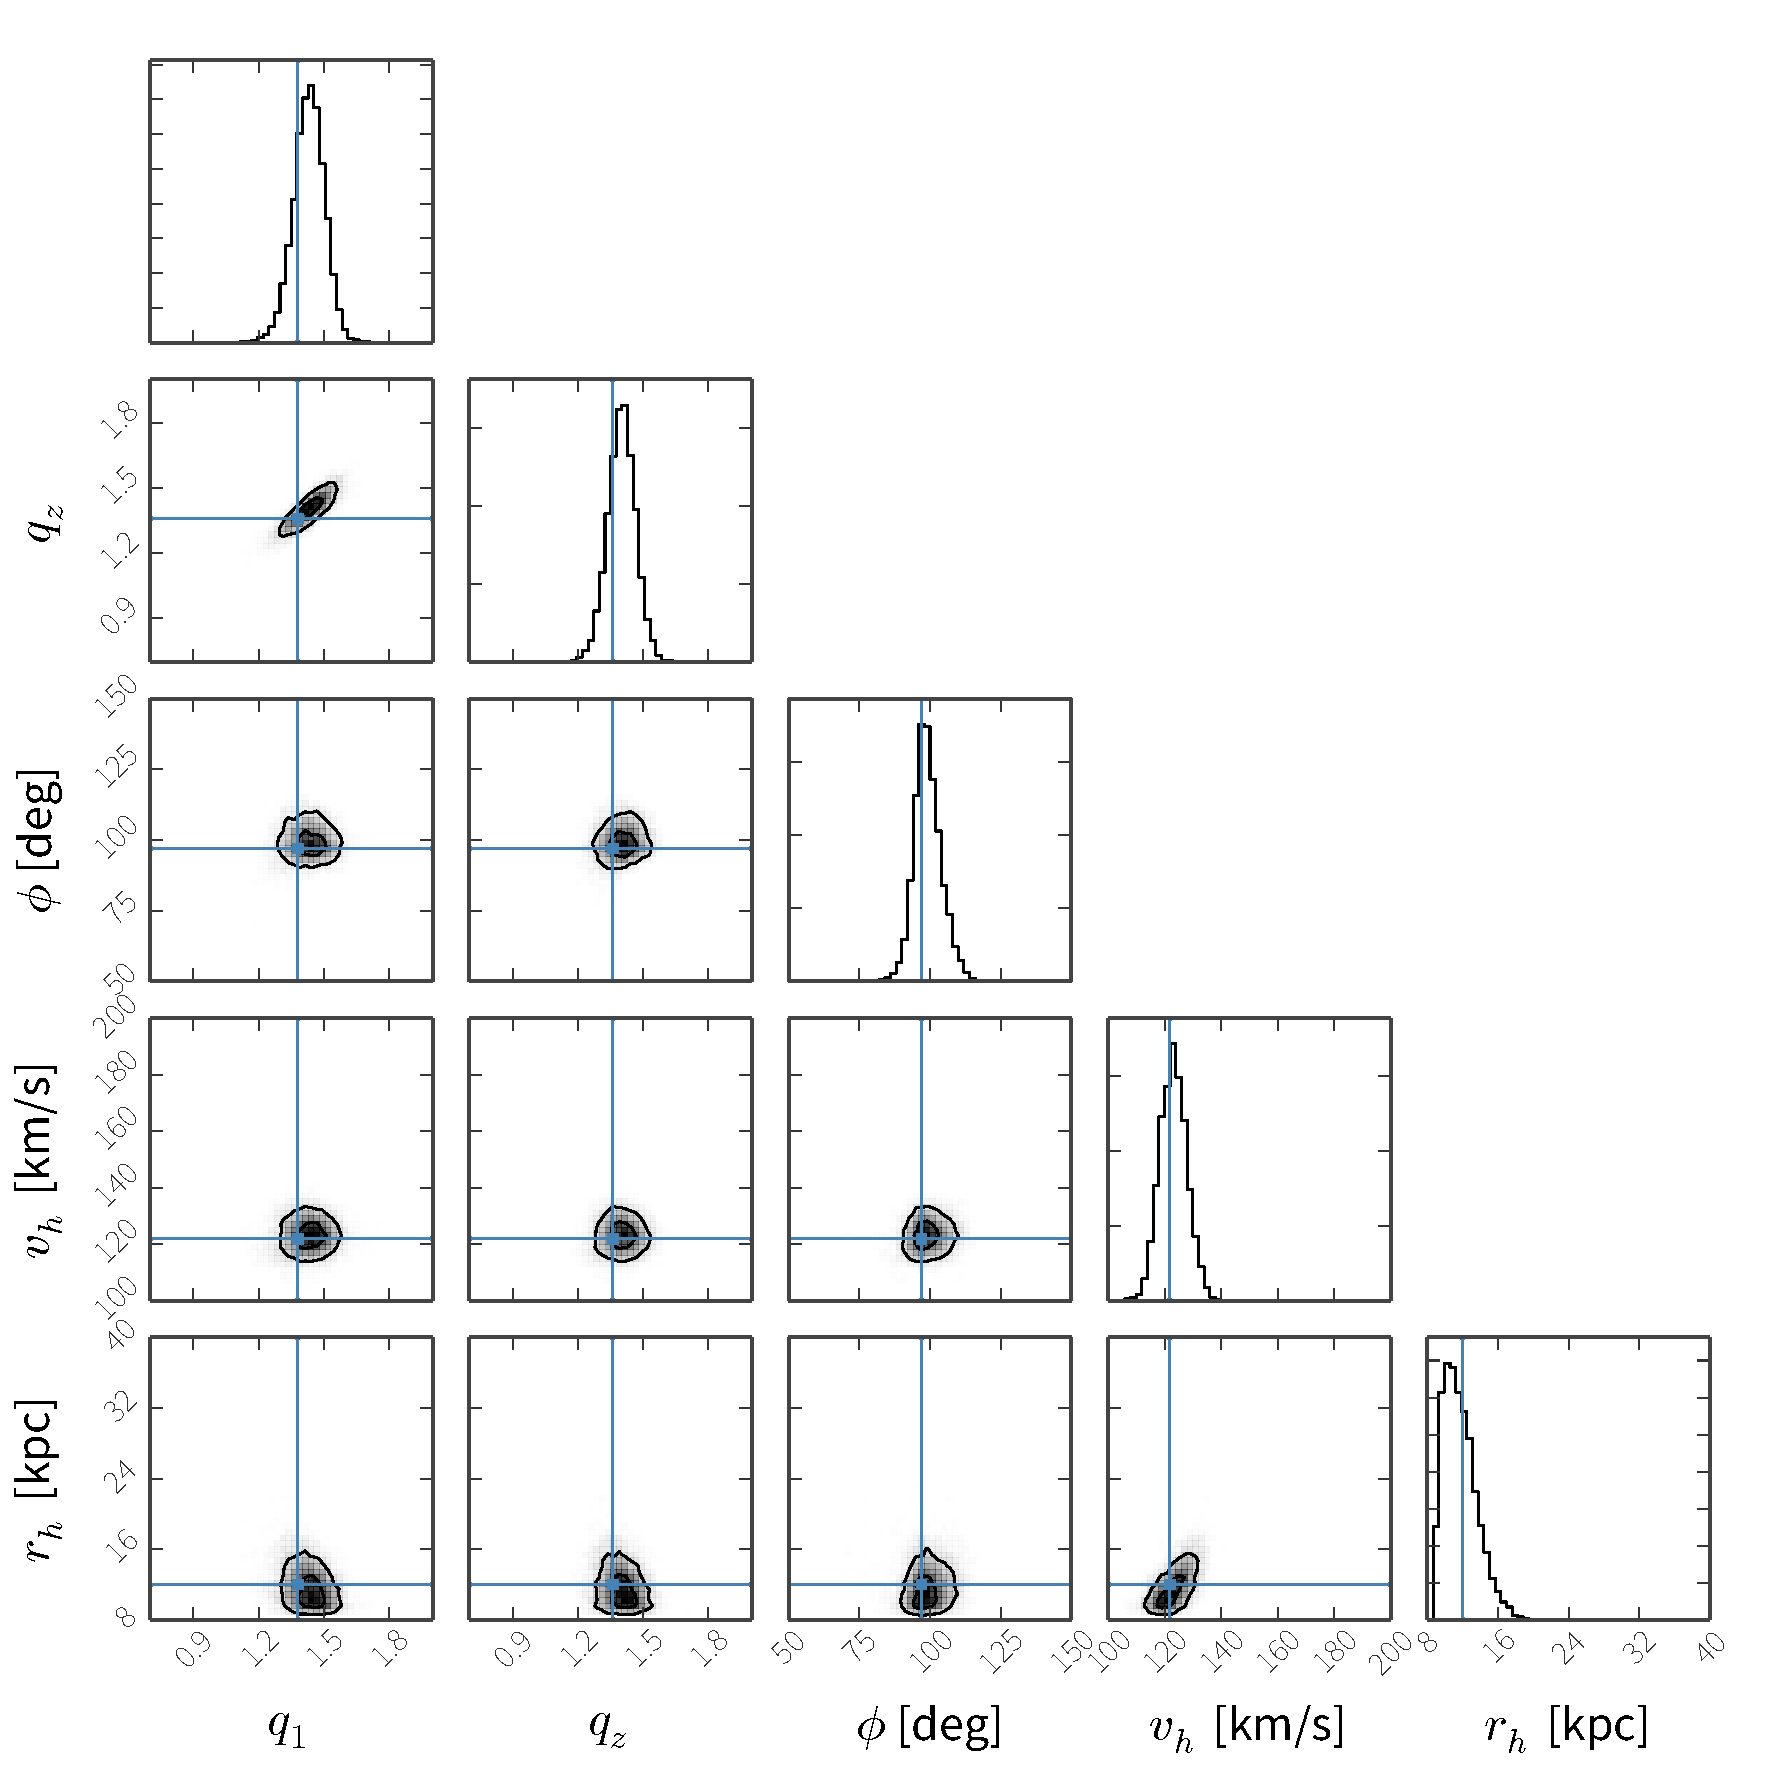
\includegraphics[width=\textwidth]{figures/ch2/exp2_potential.pdf}
\caption{ Projections of the marginal posterior over the triaxial potential
parameters for observed stars and progenitor with near-future uncertainties
(Section~\ref{sec:ch3-exp2}). Axis ranges show the lower and upper bounds on the
uniform priors over these parameters. }\label{fig:exp2_potential}
\end{center}
\end{figure*}

\begin{figure*}[!h]
\begin{center}
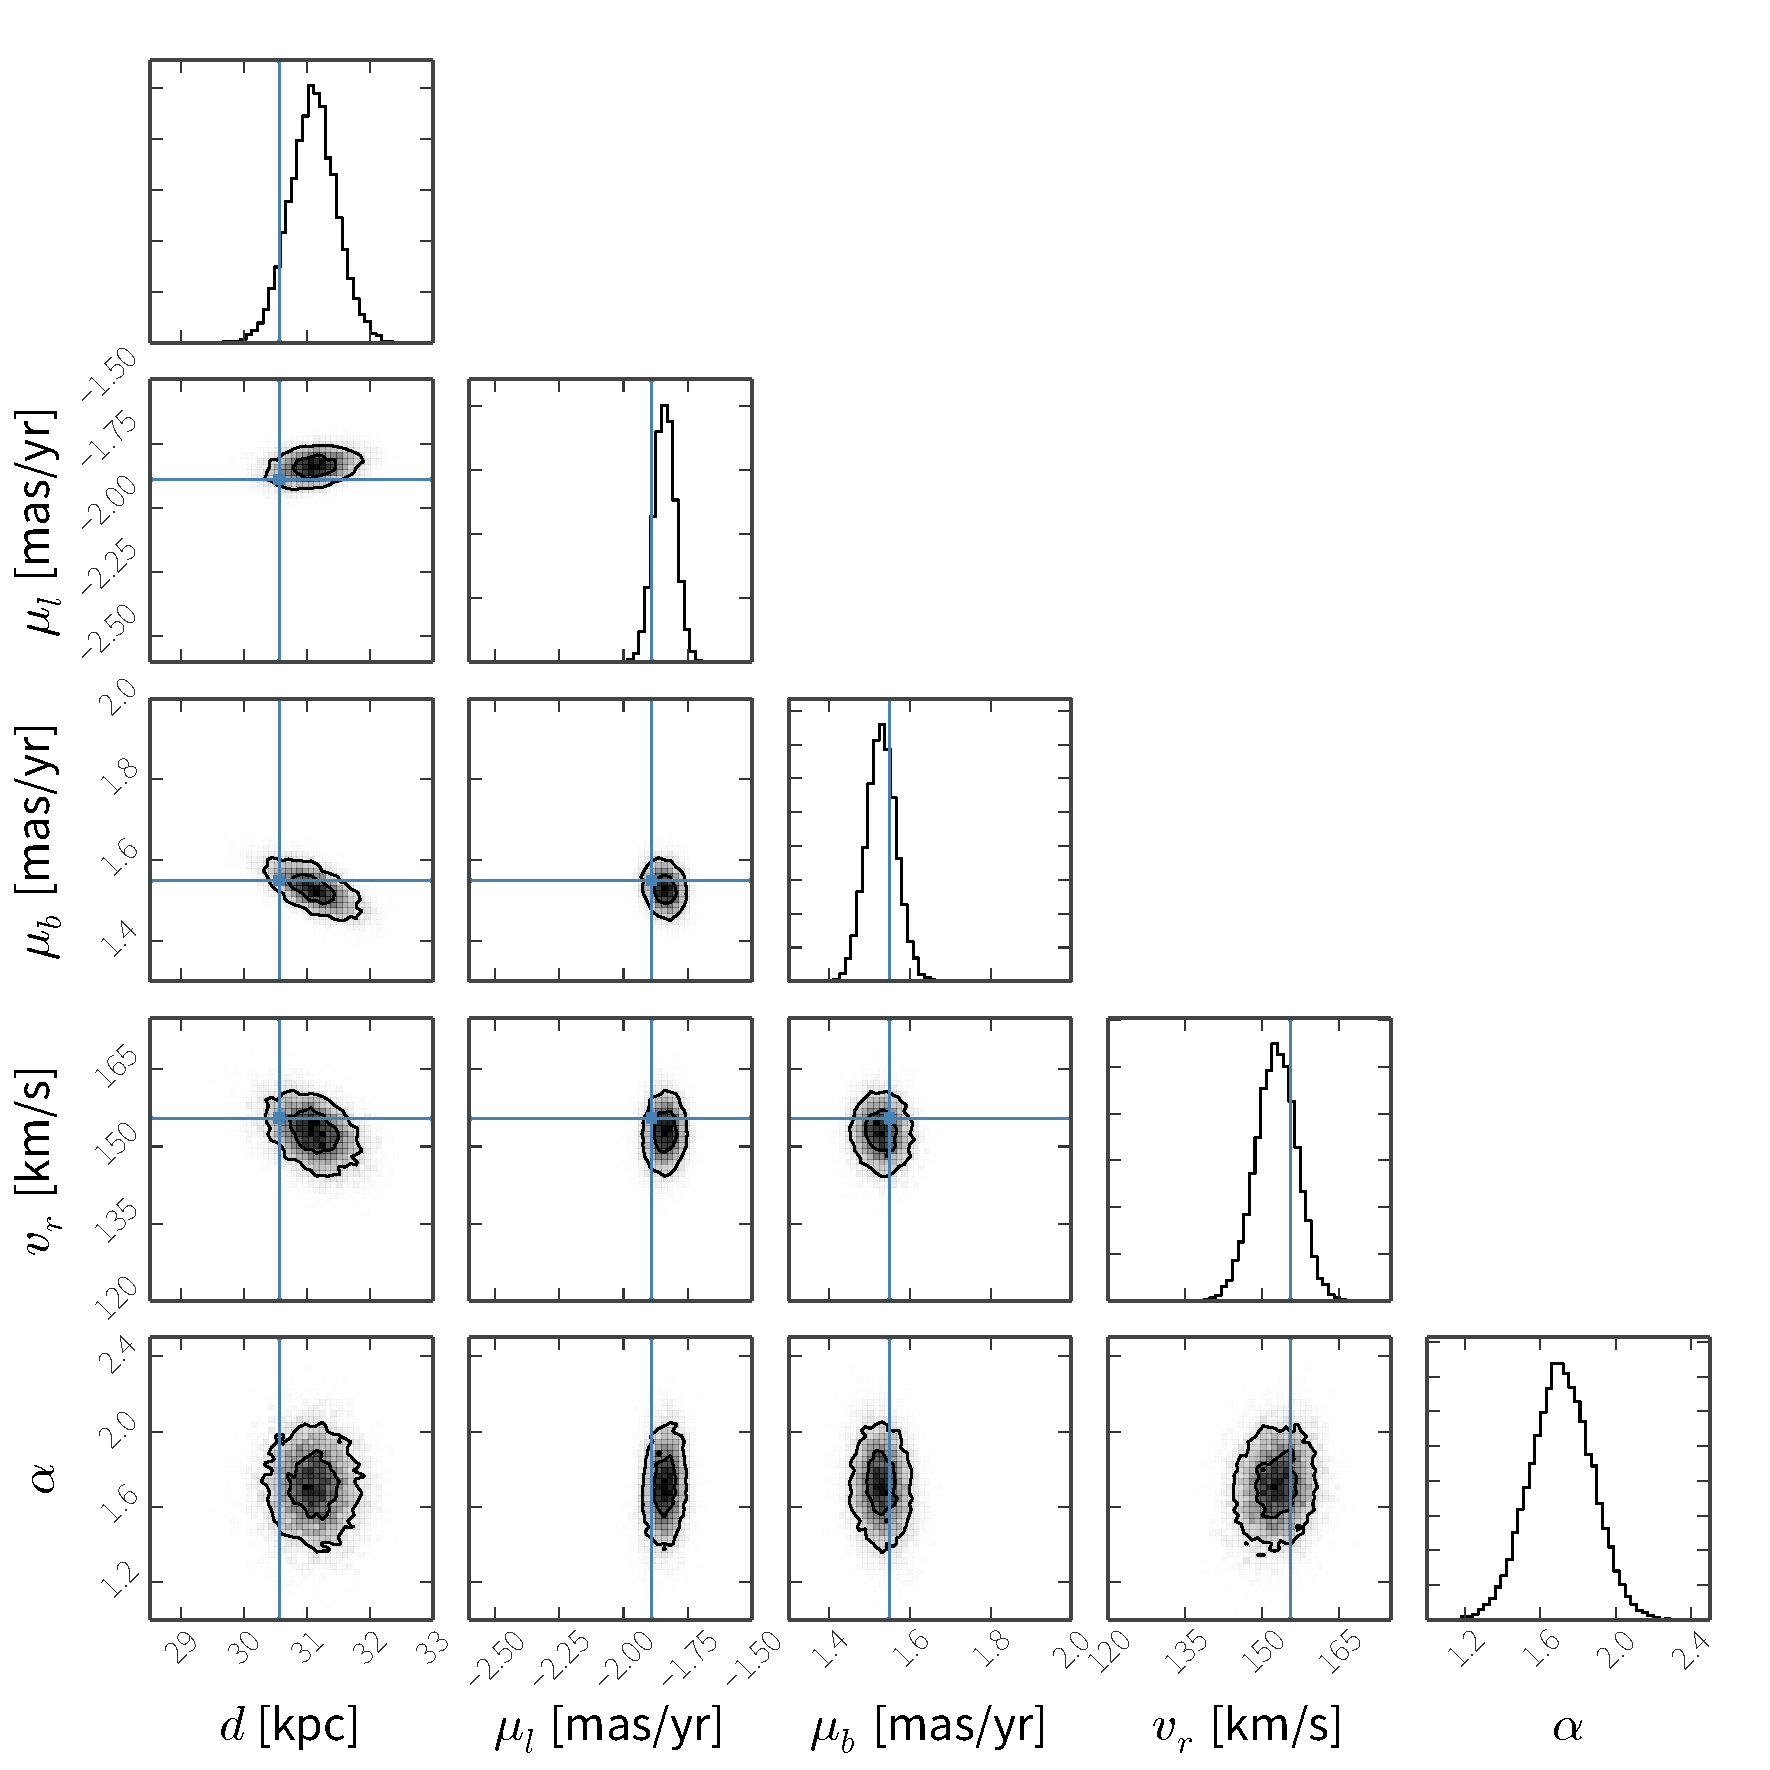
\includegraphics[width=\textwidth]{figures/ch2/exp2_satellite.pdf}
\caption{ Projections of the marginal posterior over the progenitor parameters
for observed stars and progenitor with near-future uncertainties
(Section~\ref{sec:ch3-exp2}). }\label{fig:exp2_satellite}
\end{center}
\end{figure*}

\begin{figure*}[!h]
\begin{center}
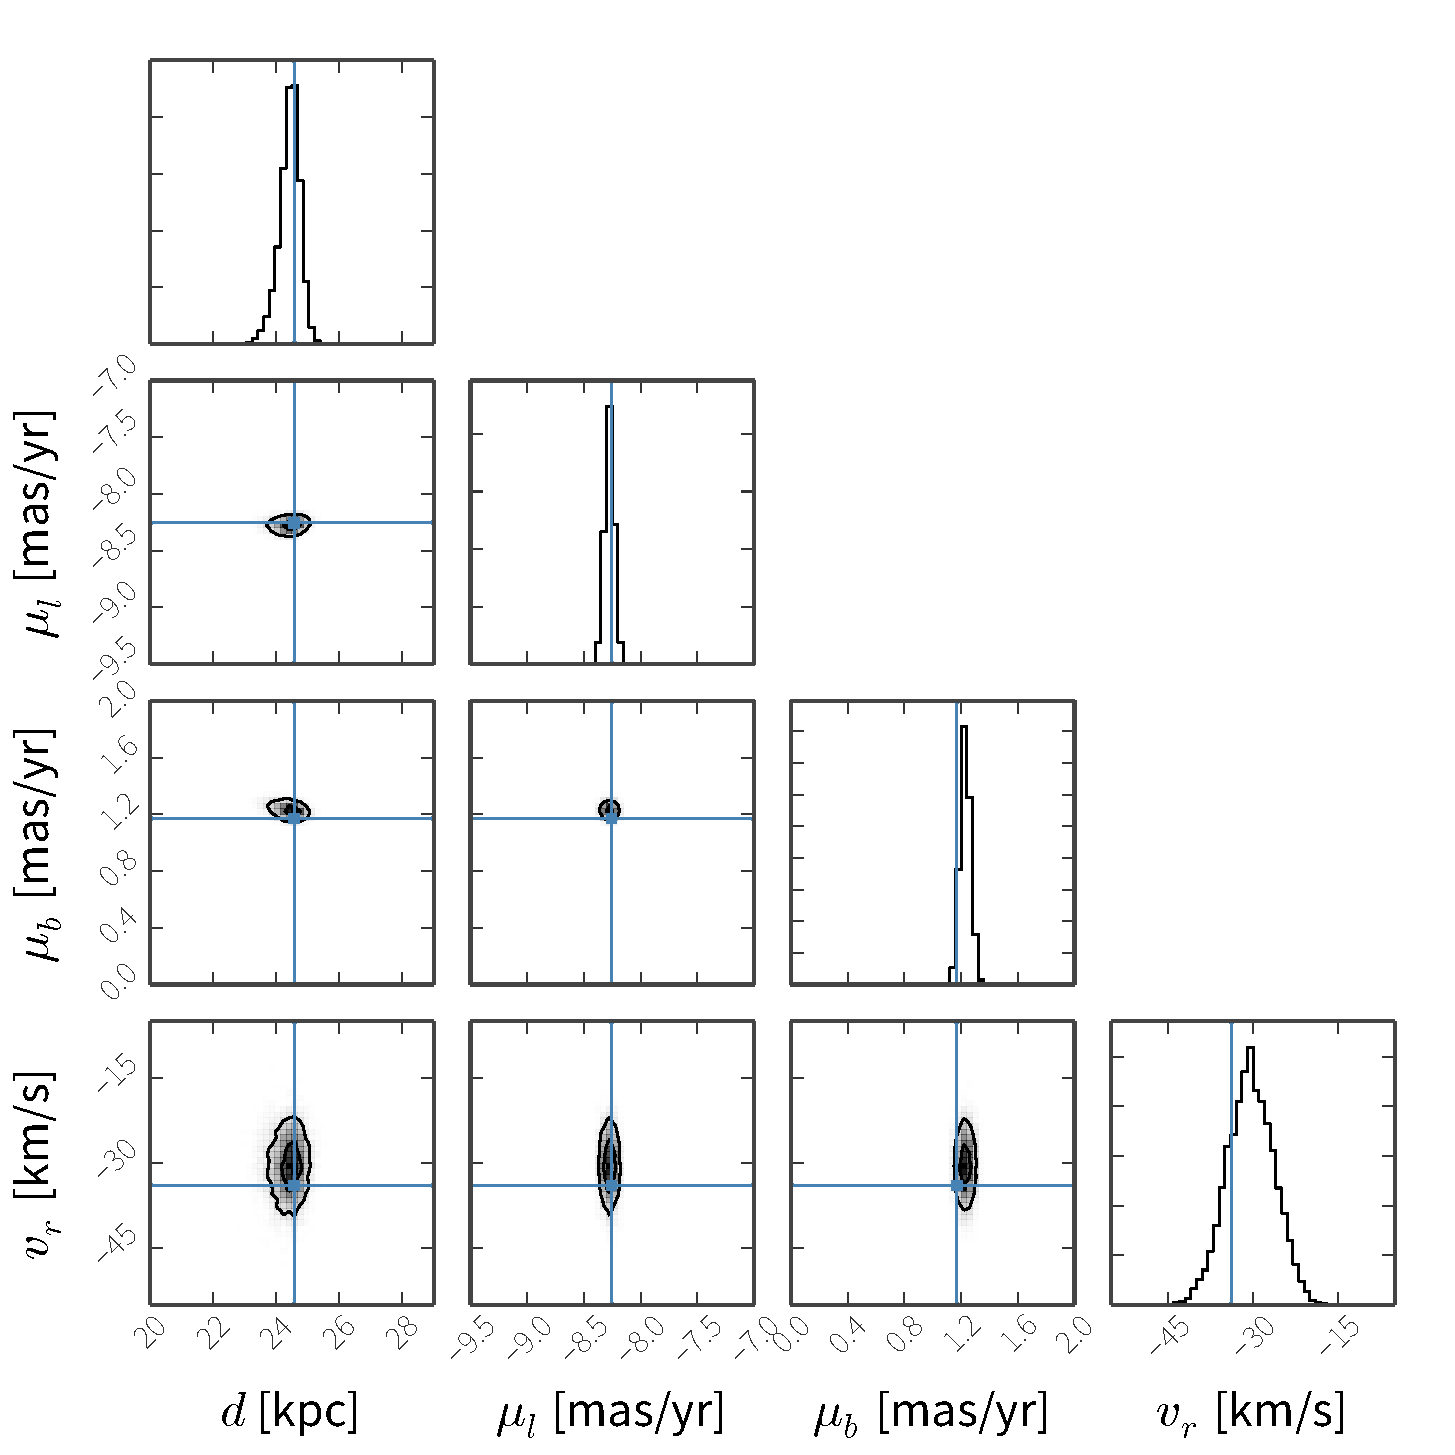
\includegraphics[width=\textwidth]{figures/ch2/exp2_particle.pdf}
\caption{ Projections of the marginal posterior over parameters for one of the
stars for observed stars and progenitor with near-future uncertainties
(Section~\ref{sec:ch3-exp2}).   }\label{fig:exp2_particle}
\end{center}
\end{figure*}

\subsection{Precise distance measurements with missing proper motions}\label{sec:ch3-exp3}
The Spitzer Merger History and Shape of the Galactic Halo survey
\citep[SMASH;][]{smashprop} will be completed within a year (early 2015), long
before the final \gaia\, data release. Thus, we will soon have precise distance
measurements for stars in the Sgr and Orphan streams, but poor or no proper
motion constraints. SMASH also targets several RR Lyrae in the Sgr core, which
will enable a high-precision distance measurement of the progenitor. We now
consider a case in which we have high-precision (2\%) distances to stream stars
and the progenitor, 10~km/s radial velocity uncertainty, and a proper motion
uncertainty for the Sgr core of $0.2~{\rm mas~yr^{-1}}$ \citep{pryor10}, but
missing proper motions for the stream stars.

As with Section~\ref{sec:ch3-exp2}, this experiment includes 41 model parameters in
total. We again use an ensemble of 256 walkers. Potential parameters and
$\Loffset$ are again initialized by drawing from the priors summarized in
Table~\ref{tbl:params}. We burn in the walkers for 50000 steps and run for
500000 inference steps. We again thin the chains by taking every $\max(t_{\rm
acor})$ sample, but here the autocorrelation time is found to be very long,
$\max(t_{\rm acor}) \approx 15000$~steps. Figures~\ref{fig:exp3_potential},
\ref{fig:exp3_satellite}, \ref{fig:exp3_particle} show the marginalized
posteriors for the potential parameters, satellite parameters, and parameters
for a single particle. Even a small sample of stars with precise distance
measurements provide an enormous amount of information about the triaxiality of
the potential. The uncertainties on the potential parameters are only 7-10\% for
the flattening and circular velocity, but $\sim$40\% for the scale radius,
$\rhalo$. The initially missing star proper-motions are recovered with
$\sim$5-10\% uncertainties.

\begin{figure*}[!h]
\begin{center}
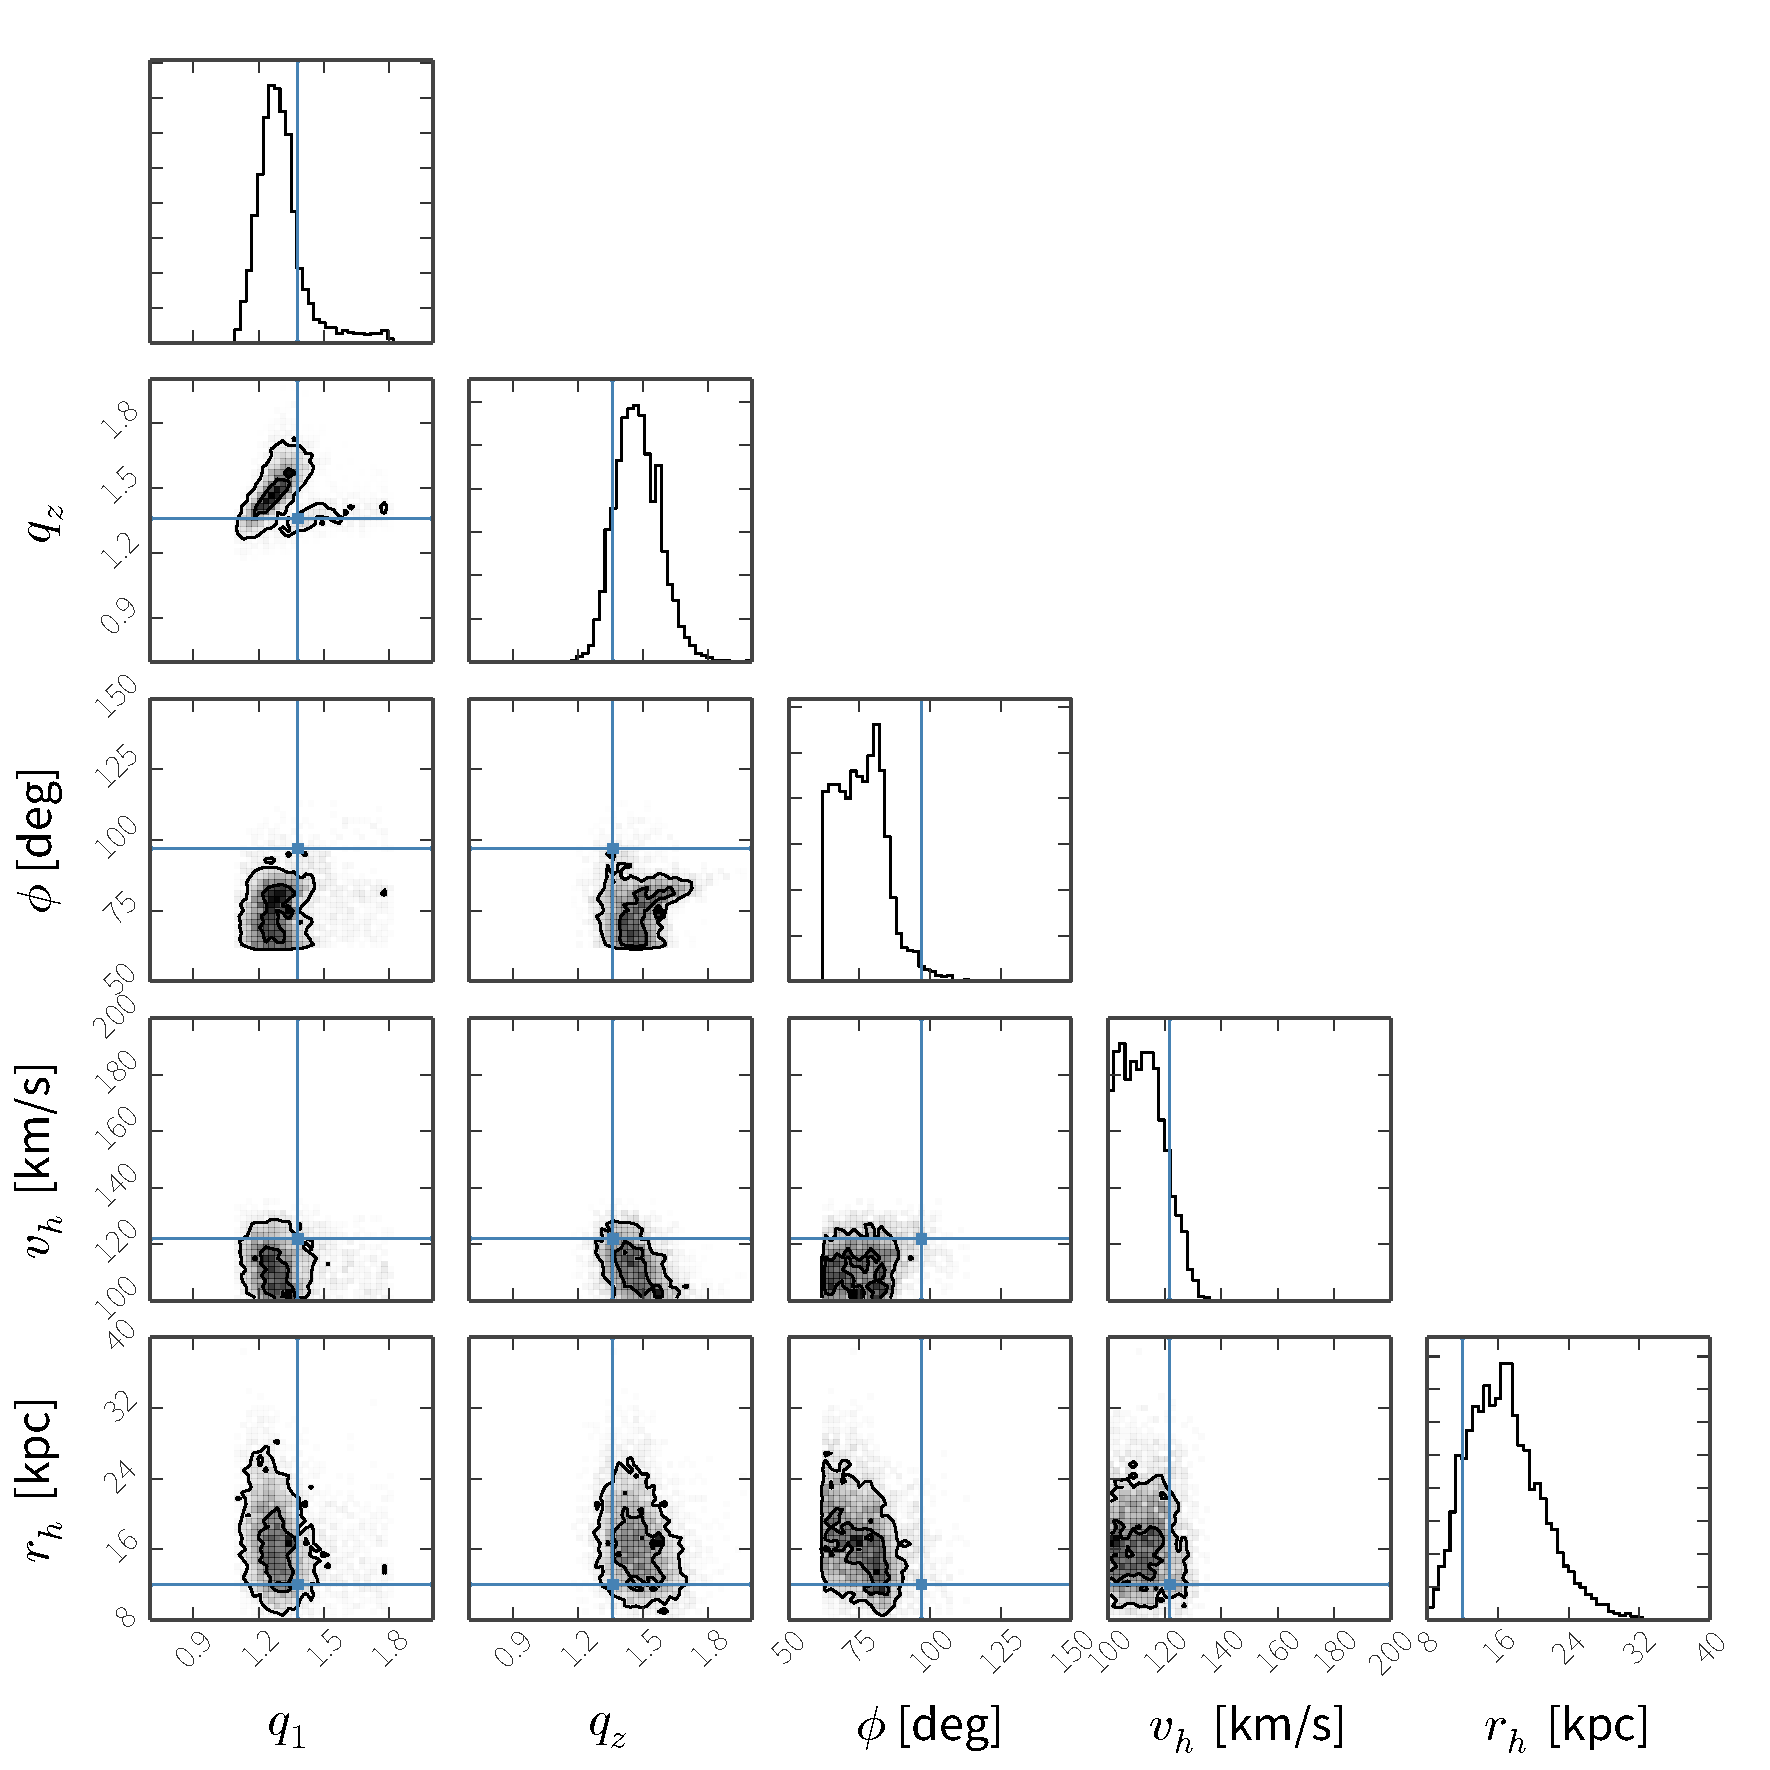
\includegraphics[width=\textwidth]{figures/ch2/exp3_potential.pdf}
\caption{ Same as Figure~\ref{fig:exp2_potential} but for data with no proper motion measurements. }\label{fig:exp3_potential}
\end{center}
\end{figure*}

\begin{figure*}[!h]
\begin{center}
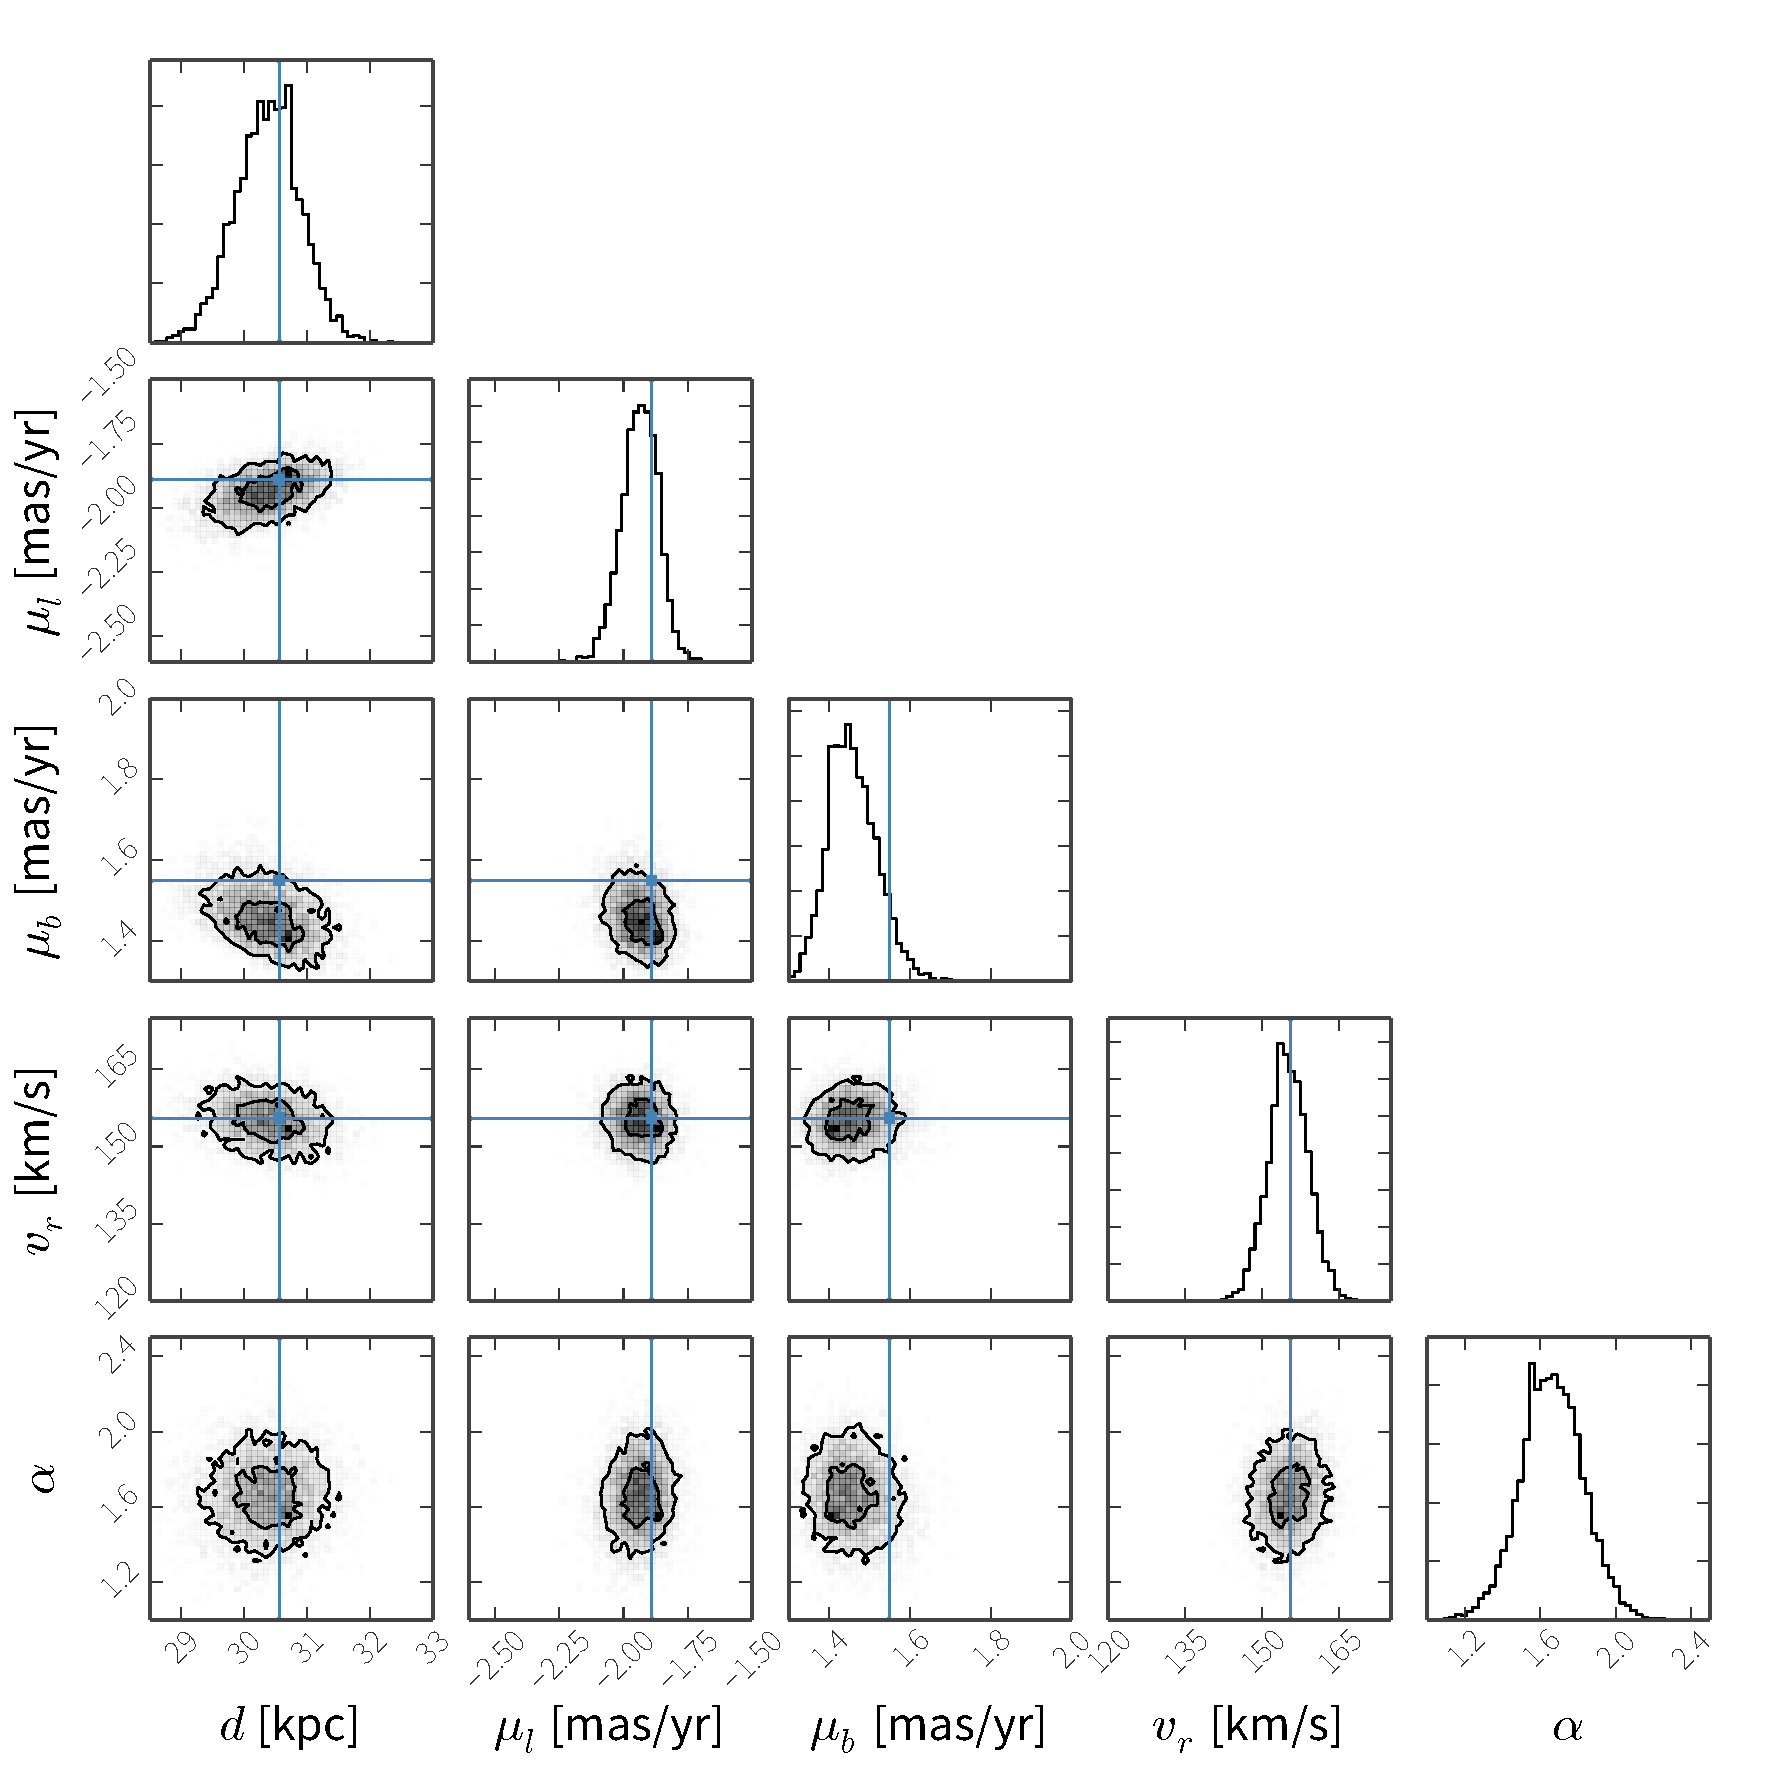
\includegraphics[width=\textwidth]{figures/ch2/exp3_satellite.pdf}
\caption{ Same as Figure~\ref{fig:exp2_satellite} but for data with no proper motion measurements.  }\label{fig:exp3_satellite}
\end{center}
\end{figure*}

\begin{figure*}[!h]
\begin{center}
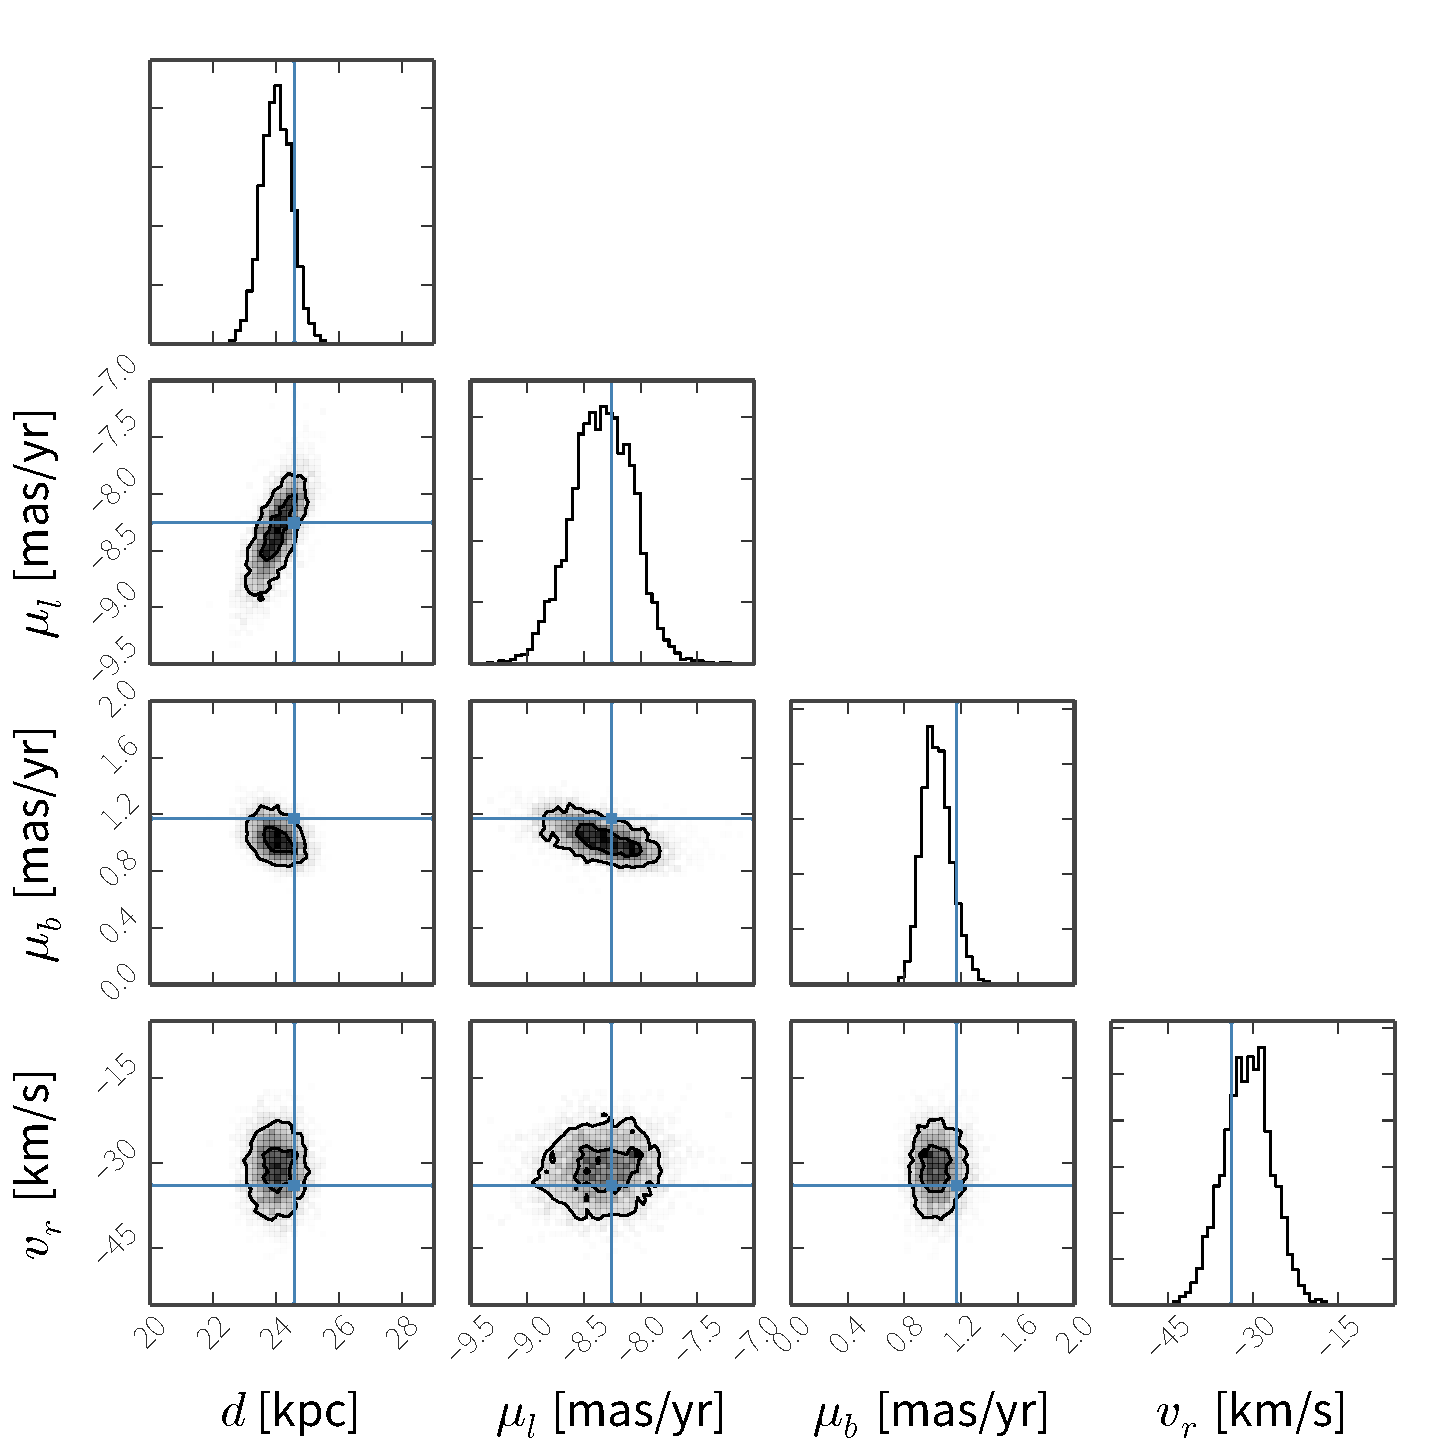
\includegraphics[width=\textwidth]{figures/ch2/exp3_particle.pdf}
\caption{ Same as Figure~\ref{fig:exp2_particle} but for data with no proper motion measurements.  }\label{fig:exp3_particle}
\end{center}
\end{figure*}

\section{Discussion}\label{sec:ch3-discussion}

{\bf 1. Observational uncertainties:} Any method that uses tidal debris as a
potential measure must also model the (significant) uncertainties on the
kinematic measurements; \rewinder\ handles observational uncertainties and
missing data dimensions by including the true 6D positions of stars and the
progenitor as model parameters. In this \article\ we have tested \rewinder\
using data of varied quality for a small sample of stars.

{\bf 2. Form of the potential:} No assumptions were made about the the form of
the Galactic potential in deriving the likelihood for \rewinder. The simple
experiments in this \article\ infer potential parameters from the same static,
analytic potential used in the $N$-body simulations that generated the fake data.
However, in principle the potential could be time-dependent, clumpy, or have
properties that vary with radius. The orbits of the stars and progenitor are
directly integrated and only require a function that evaluates the acceleration
due to the potential at a given position (and time). We have shown that with the
correct form for the Galactic potential, \emph{precise} measurements of the
potential parameters are attainable with near-future data, but we have not
discussed the \emph{accuracy} of such measurements due to incorrect assumptions.
For example, \citep{bonaca14} show that using a static potential model to fit
the live potential of the \project{Via Lactea} halo with tidal streams can
introduce significant biases to measurements of the halo mass, even with perfect
knowledge of the 6D coordinates of stars in the streams. In future work, we will
(1) try fitting incorrect potential models to see if we can still recover global
properties (e.g., flattening); (2) run simulations with smoothly changing
potentials \citep[e.g.,][]{buist14} and attempt to model the time dependence;
and (3) explore using a generic, non-parametric potential form (e.g., a basis
function expansion) as the recovery potential model.

{\bf 3. Multiple debris structures:} Each stream will provide constraints on
different properties of the potential. For example, more eccentric streams may
better constrain the radial profile \citep[see][who illustrate the power of
using multiple streams to simultaneously constrain the potential using orbit
fitting]{deg14}. In this \article, we only consider a stream on a Sgr-like orbit,
which lies nearly in the Galactic $x$-$z$ plane. We find that the stream puts
better constraints on the $z$-axis flattening, $q_z$, than on the flattening in
the $x$-$y$ plane, $q_1$, as one might expect. The best measurements of the
detailed shape of the Galactic potential will come from combining constraints
from multiple streams. We have defined above a proper likelihood function for
observed stars in a given stream, thus incorporating multiple streams into the
inference only requires multiplying the likelihoods computed for each stream and
progenitor pair.

{\bf 4. Comparing models to data:} With \rewinder, each star adds constraints on
the potential parameters and does not require matching a simulated density to
the observed density of stars, thus this method works well even for small
samples of well-measured stream stars. It might be that the most relevant
stellar samples for inferring the Milky Way potential are small. For instance,
stars that produce good distance estimates might be much more valuable than
typical stars in the sample so that we may limit to only variable stars, e.g.,
RR Lyraes. These valuable stars are rare (and their abundances are age and
metallicity dependent); there could be many cold structures in the Milky Way
halo that are highly constraining on the potential in principle, but which
contain only a few good distance-indicating members. It is not yet known what
the trade-offs are between having many stars at low precision and a few at high
precision, nor is it known how valuable distance information really is, when a
structure contains many precisely observed members.

{\bf 5. Computational expense:} One point of concern for \rewinder\ is that the
number of parameters scales with eight times the number of stars: each star has
six coordinate parameters (the true position), the unbinding time, and the tail
assignment. Computational constraints limit the sample size, but even so, the
inference is much faster than full $N$-body modeling because the stars and
progenitor are treated as test particles. Each step in parameter space with
\rewinder\ requires integrating the orbits of stars and the progenitor: we
presently integrate with a fixed time-step using leapfrog integration. Computing
the acceleration due to the given potential at each step is implemented in
\texttt{Cython} (and approaches \texttt{C}-like speed), but the rest of the code
is written in pure-\python. Though already significantly less
computationally intensive than running a full $N$-body simulation for every
parameter step, running each MCMC walker for $\gtrsim$100000 steps requires
parallelization a few hours of CPU time on a compute cluster. Further
optimization of the integration method (e.g., using an adaptive method or
implementing in \texttt{Cython}) could speed up the inference significantly.

\section{Conclusions}\label{sec:ch3-conclusion}
We have presented a probabilistic model (\rewinder)---a likelihood function and
with priors on the parameters---for using stars observed in tidal streams to
constrain properties of any underlying gravitational potential. \rewinder\
relies on direct orbit integration and not on computing conserved quantities
(e.g., actions) and can thus be used with arbitrarily complex (e.g.,
time-dependent or clumpy) forms of the potential. We have performed several
experiments to show that \rewinder\ simultaneously constrains the potential and
models a tidal stream given simulated data with a range of realistic
uncertainties. We find that with future high-quality data---that is, high
precision distance measurements from RR Lyrae and proper motions from \gaia---a
small sample of just eight stars in a tidal stream modeled with \rewinder\,
provide measurements of potential parameters that rival present-day constraints
from comparing full $N$-body simulations to large numbers of stellar tracers with
poorly measured kinematics. For this high-quality data, we recover the input
potential parameter values with uncertainties of order 5-7 percent. Without
proper motion data the uncertainties range from 10-40 percent. We consider this
work to be an encouraging first step towards the goal of recovering the
(presumably) much more complex---time-dependent, clumpy, with axis ratios and
orientations that vary with radius---Milky Way potential with larger data sets.

\section*{Acknowledgments}
We thank Anthony Brown (Leiden) for insight on the \gaia\, data quality and for
providing the open source \project{PyGaia} code for computing predicted
uncertainties. We thank the organizers of the Gaia Challenge (2013) and the
University of Surrey for hospitality during the workshop. We thank Ana Bonaca
(Yale), Jo Bovy (IAS), Dan Foreman-Mackey (NYU), Marla Geha (Yale), Andreas
K{\"u}pper (Columbia), and Hans-Walter Rix (MPIA) for useful discussions. KVJ
thanks the Institute of Astronomy at the University of Cambridge for hospitality
and Vasily Belokurov (IoA) and his group for discussion of his work while there.
APW is supported by a National Science Foundation Graduate Research Fellowship
under Grant No.\ 11-44155. This work was supported in part by the National
Science Foundation under Grant No. PHYS-1066293 and AST-1312196. DWH was
partially supported by the NSF (Grant IIS-1124794) and the Moore-Sloan Data
Science Environment at NYU. This research made use of Astropy, a
community-developed core \python\ package for Astronomy
\citep{astropy13}. This research has made use of NASA's Astrophysics Data
System. This work additionally relied on Columbia University's \emph{Hotfoot}
and \emph{Yeti} compute clusters, and we acknowledge the Columbia HPC support
staff for assistance.

	\chapter[Chaotic dispersal of tidal debris]{Chaotic dispersal of tidal debris \label{ch:chaos-morphology}}
\let\thefootnote\relax\footnotetext{This section contains text from an article published in Monthly Notices of the Royal Astronomical Society, Volume 455, Issue 1, p.1079-1098 (2016).}

% More definitions for this chapter
\newcommand{\chchchanges}[1]{#1}
\newcommand{\inttime}{t_{\rm int}}
\newcommand{\periods}{\ensuremath{{\rm T}}}
\newcommand{\act}{J}
\newcommand{\jac}{\mathscr{J}}

%\begin{document}
%
%\title{Chaotic dispersal of tidal debris}
%\author{Adrian M. Price-Whelan\altaffilmark{\colum,\adrn},
%	    Kathryn V. Johnston\altaffilmark{\colum},
%	    Monica Valluri\altaffilmark{\mich},
%	    Sarah Pearson\altaffilmark{\colum},
%	    Andreas H. W. K\"upper\altaffilmark{\colum,\hubble},
%	    David W. Hogg\altaffilmark{\nyu,\cds,\mpia}}
%%\date{\centering \today}
%
%% Affiliations
%\newcommand{\colum}{1}
%\newcommand{\adrn}{2}
%\newcommand{\mich}{3}
%\newcommand{\hubble}{4}
%\newcommand{\nyu}{5}
%\newcommand{\cds}{6}
%\newcommand{\mpia}{7}
%\altaffiltext{\colum}{Department of Astronomy,
%		              Columbia University,
%		              550 W 120th St.,
%		              New York, NY 10027, USA}
%\altaffiltext{\adrn}{To whom correspondence should be addressed: adrn@astro.columbia.edu}
%\altaffiltext{\mich}{Department of Astronomy,
%			   University of Michigan,
%			   Ann Arbor, MI 48109, USA}
%\altaffiltext{\hubble}{Hubble fellow}
%\altaffiltext{\nyu}{Center for Cosmology and Particle Physics,
%                      Department of Physics, New York University,
%                      4 Washington Place, New York, NY, 10003, USA}
%\altaffiltext{\cds}{Center for Data Science,
%                      New York University,
%                      4 Washington Place, New York, NY, 10003, USA}
%\altaffiltext{\mpia}{Max-Planck-Institut f\"ur Astronomie,
%                     K\"onigstuhl 17, D-69117 Heidelberg, Germany}
%
%\begin{abstract}
%
%Several long, dynamically cold stellar streams have been observed around the Milky Way Galaxy, presumably formed from the tidal disruption of globular clusters.
%In integrable potentials---where all orbits are regular---tidal debris phase-mixes close to the orbit of the progenitor system.
%However, the Milky Way's dark matter halo is expected not to be fully integrable; an appreciable fraction of orbits will be chaotic.
%This paper examines the influence of chaos on the phase-space morphology of cold tidal streams.
%\chchchanges{Streams even in weakly chaotic regions look very different from those in regular regions.}
%We find that streams can be sensitive to chaos on a much shorter time-scale than any standard prediction (from the Lyapunov or frequency-diffusion times).
%For example, on a weakly chaotic orbit with a chaotic timescale predicted to be $>$1000 orbital periods ($>$1000 Gyr), the resulting stellar stream is, after just a few 10's of orbits, substantially more diffuse than any formed on a nearby but regular orbit.
%We find that the enhanced diffusion of the stream stars can be understood by looking at the variance in orbital frequencies of orbit ensembles centered around the parent (progenitor) orbit.
%Our results suggest that long, cold streams around our Galaxy must exist only on regular (or very nearly regular) orbits; they potentially provide a map of the regular regions of the Milky Way potential.
%This suggests a promising new direction for the use of tidal streams to constrain the distribution of dark matter around our Galaxy.
%
%\end{abstract}
%
%\keywords{
%}

\section{Introduction}\label{sec:ch4-introduction}

The dark-matter haloes of galaxies are thought to be triaxial in shape with axis
ratios and alignments that depend on radius. However, despite suggestive
evidence from a range of complimentary observational methods, this fundamental
prediction from $\Lambda$CDM cosmology has not been conclusively verified.
Around other galaxies, it is generally hard to measure the 3D mass profile
because informative tracers are rare and the haloes are seen in projection. From
the Earth's position within the Milky Way, our view of our own halo and
proximity gives us a unique chance to directly measure the 6D positions of stars
and model the shape of the mass distribution at large radii. The Milky Way halo
has a low density of visible tracers, but luckily many of the halo stars are
likely associated with debris stripped from stellar systems and thus contain
additional information encoded by the formation mechanism.

As a satellite galaxy or globular cluster orbits within some larger system, mass
is eroded by tidal forces from the host-galaxy potential. Along regular, mildly
eccentric orbits, mass stripped from the progenitor has a small spread in
orbital properties (e.g., energy, angular momentum). Once the debris has evolved
far enough from the progenitor system that the self-gravity of the progenitor
can be ignored (usually a fast process relative to the orbital time), the stars
evolve essentially as an ensemble of test particle orbits in the potential of
the host system. The debris remains coherent as a tidal stream if the
phase-mixing time-scale is long: a small ensemble of regular orbits reaches a
fully phase-mixed state in a timescale $\approx\sigma_\Omega^{-1}$, where
$\sigma_\Omega$ is the dispersion in fundamental frequencies of the ensemble
(tidal debris from a globular cluster typically has frequency spreads
$\approx$0.1--1\%, so it can take hundreds to thousands of orbital periods to
fully phase-mix). The ensemble spreads due to shearing from slight variations in
their fundamental frequencies, which, for tidal streams, preferentially occurs
along one dimension \citep{merritt96, helmi99}.

The morphological (density) evolution of the tidal debris therefore depends on
the spread of orbital properties (e.g., actions or frequencies) of the debris
and the orbit of the progenitor system, both of which are also determined by the
shape and radial profile of the gravitational potential of the host galaxy. By
modeling the observed phase-space density of stream stars along with the host
galaxy potential it is hoped that we may infer the 3D mass distribution of the
host. Many tidal streams are observed around the Milky Way, M31, and other
nearby galaxies; the known streams span a large range of distances---from
$\approx10$ to $100~{\rm kpc}$---and progenitor masses---from $\approx$10$^3$ to
$\approx$10$^8~\msun$ in stellar mass---\citep[][]{ibata94,odenkirchen01,
belokurov06,grillmair06a,grillmair06b,bonaca12}. There has been extensive work
on developing methods to use data from these streams to measure properties of
the Milky Way's dark matter halo. These methods span a range of complexity from
orbit-fitting, to \emph{Streakline} \citep{kuepper12} or `particle-spray' models
\citep{gibbons14}, to action-space density modeling \citep[e.g.,][]{sanders14,
bovy14}, to $N$-body simulations \citep[e.g.,][]{law10}. All methods have been
tested in some way on simulated observations of data and these tests typically
demonstrate the recovery of parameters for analytic, static potential forms.

One example of stream modeling in a multi-component (static, analytic) potential
was presented by \citet{pearson15}, who aimed to reproduce observations of the
stellar stream density from the globular cluster Palomar 5 in a single oblate
and single triaxial potential using \emph{Streakline} \citep{kuepper12} and
$N$-body models. They used the observed number density of stream stars, a limited
number of radial velocities for stream members, and the sky position, distance,
radial velocity, and proper motion of the cluster itself to fit model streams to
the data. In the oblate potential (a three-component bulge+disk+spherical halo
potential), a thin model stream was easily found that reproduces the observed
stellar density morphology of the stream. In the triaxial potential (the
potential from \cite{law10}: a three component bulge+disk+triaxial halo fit to
Sagittarius stream data), the model streams generically formed large,
two-dimensional `fans' of debris near the ends, and no physically reasonable
progenitor orbits could be found that reproduced the observed thinness and
curvature of the stream given the observational constraints of the present-day
position and velocity of the cluster. The result in \citet{pearson15}
demonstrates that the morphology of a stream alone can be used to rule out a
potential. With an understanding of the circumstances that lead to the
differences in stream morphology, this could be a powerful tool for rejecting
potentials from positional information alone.

The obvious difference between the two potentials considered by
\citet{pearson15} is the extra symmetry of the oblate potential. It is well
known that the number of degrees of freedom of a potential plays a critical role
in determining the orbit structure of the potential; Hamiltonians with more than
two degrees of freedom generically contain significant chaotic regions.
\citet{pearson15} tested the stochasticity of the orbit of the progenitor that
produced `fanned' debris by computing the Lyapunov exponent along this orbit but
found that it is consistent with being regular over dynamically relevant
timescales (many Hubble times). It has been shown previously that along some
strongly chaotic orbits and in live cosmological haloes, tidal streams do form
large, diffuse `fans' of debris \citep[e.g.,][]{fardal14, ngan15}, however it is
unknown how the resultant properties of the debris (e.g., density or length of
the stream) depend on the degree of stochasticity. The result from
\citet{pearson15} suggests that even weak chaos (as measured by the Lyapunov
exponent) may affect the density evolution and therefore observability of tidal
streams. Understanding why this occurs and developing a measure to quantify the
importance of this enhanced density evolution is a promising new direction to be
explored further.

In this \article, we study the effect of chaotic diffusion of the
fundamental frequencies of individual orbits on the density evolution of tidal
debris. We choose a simple, cosmologically motivated model for a triaxial
potential, analyze the degree of chaos as computed from single-orbit diagnostics
for grids of constant-energy orbits, and compare these results to measures of
the density evolution of finite-volume ensembles of orbits (meant to mimic tidal
debris). We find that even when the chaotic timescale is predicted to be long
for a given orbit, chaos may manifest over much shorter times in small orbit
ensembles through the chaotic diffusion of the constituent orbits. For a chaotic
orbit, the frequency spectrum of the orbit evolves with time: for a small
ensemble, the spread in frequencies is therefore time-dependent, which could
enhance phase-mixing. This idea supports a reevaluation of the importance of
chaos in galactic haloes and implies that the amount of chaos in a given
potential may have significant consequences for the observability and
survivability of thin, cold tidal streams.

This \article\ is organized as follows. We review relevant nonlinear dynamics in
Section~\ref{sec:ch4-nldreview}. In Section~\ref{sec:ch4-methods}, we describe our
choice of potential, method for numerical orbit integration, and introduce the
chaos indicators used in this work. Our results are split into three
subsections: in Section~\ref{sec:ch4-results1} we present iso-energy grids of orbits
and discuss the orbit classes and chaotic timescales present in our potential;
in Section~\ref{sec:ch4-results2} we study the density evolution of small ensembles
of orbits around each orbit of the previous section; in
Section~\ref{sec:ch4-results3} we describe the behavior of chaotic diffusion and use
this to explain how chaos is relevant for tidal streams over short times. We
discuss the implications of our results in Section~\ref{sec:ch4-discussion}, and
conclude in Section~\ref{sec:ch4-conclusions}.

\section{Review of nonlinear dynamics}\label{sec:ch4-nldreview}

To explore the question of if and how chaos manifests in the density evolution
of orbit ensembles over timescales much shorter than that predicted from generic
chaos indicators, we must first understand the behavior of individual orbits in
complex gravitational potentials and the orbital structures in the potential
itself (i.e. the strength of resonances and chaos). An orbit in an $N$ degree of
freedom (dof) Hamiltonian, $H$, is a set of $2N$ quasi-periodic time series,
\begin{equation}
(w_1(t),...,w_{2N}(t)) = (q_1(t),...,q_{N}(t),p_1(t),...,p_{N}(t)) \label{eq:coords}
\end{equation}
where $q_k$ and $p_k$ are conjugate coordinates in the sense that
\begin{align}
	\dot{p}_k &= -\frac{\partial H}{\partial q_k}\\
	\dot{q}_k &= \frac{\partial H}{\partial p_k}
\end{align}
for all $t$. If bounded, the motion in any component, $w_k(t)$, can be described as a Fourier sum,
\begin{equation}
	w_k(t) = \sum_j^\infty a_{kj} \, e^{i\,\omega_j\,t} \label{eq:fourier}
\end{equation}
where the $a_{kj}$ are complex amplitudes.

A \emph{regular orbit} is a set of such time series that can be transformed to a
special set of canonical coordinates known as angle-action coordinates. In these
coordinates, the position variables are angles, $\boldsymbol{\theta}$, that
increase linearly with time with rates set by $N$ constant, fundamental
frequencies, $\boldsymbol{\Omega} = (\Omega_1, ..., \Omega_N)$. The frequency of
a Fourier component (the $\omega_k$ in Equation~\ref{eq:fourier}) for any
individual component of motion are just linear, integer combinations of the
fundamental frequencies, $\boldsymbol{\Omega}$---that is, for a regular orbit,
any Fourier component frequency may be written
\begin{align}
	\omega_j &= \boldsymbol{n_j} \cdot \boldsymbol{\Omega} \label{eq:fourierfreq}
\end{align} %; \, (\boldsymbol{n}_k \in \mathbb{Z}^3)
where $\boldsymbol{n}_k$ is a vector of $N$ integers. The conjugate momentum coordinates---the actions,  $\boldsymbol{J}$---are constants of motion. Even stronger, the actions are isolating integrals and any pair are in involution such that
\begin{equation}
	[J_\alpha, J_\beta] = 0
\end{equation}
where $[\cdot,\cdot]$ is the Poisson bracket. This implies that for an $N$ dof
system, a regular orbit has $N$ independent constants of motion and the motion
is therefore restricted to an $N$-dimensional manifold embedded in the 2$N$
dimensional phase space. The topology of angle-action space is toroidal and any
regular orbit in an $N$ dof Hamiltonian can be understood as motion on the
surface of an $N$-torus. Each set of actions, $(J_1,...,J_N)$ (or frequencies),
labels a torus, and regular orbits are sometimes referred to in terms of their
orbital tori (see, e.g., Section 50 in \citealt{arnold78}, Section 10-5 in
\citealt{goldstein80}, Section 3.5 in \citealt{binneytremaine}).

\subsection{Orbits in integrable potentials}

A Hamiltonian or potential is said to be \emph{globally integrable} when the
number of isolating integrals of motion is equal to the number of degrees of
freedom and a transformation to angle-action coordinates may be done
globally---for example, the transformation to angle-action coordinates may be
written as a function of arbitrary phase-space coordinates and the functional
form is independent of phase-space position \citep[e.g.,][]{goldstein80}. The
condition for global integrability is very restrictive and the likelihood that a
Hamiltonian is globally integrable decreases as the number of degrees of freedom
increase \citep[e.g.,][]{lichtenberg83} and as the potential becomes more
complex (i.e. containing multiple components with different shapes). In a
globally integrable potential, the Hamiltonian may be written solely in terms of
the actions, $H = H(\boldsymbol{J})$. Galactic potentials are almost certainly
not globally integrable but it is useful to understand the orbit structure in
integrable systems before extending to more general potentials. \chchchanges{For
example, there are four general classes of orbits in the `Perfect Ellipsoid'
potential \citep[an integrable triaxial potential and special case of the
St\"ackel potential; see, e.g.,][]{kuzmin73, deZeeuw85}: box, inner long-axis
tube, outer long-axis tube, and short-axis tube orbits. Regular orbits in
non-integrable triaxial potentials can typically still be identified with these
classes. Tube orbits have a non-zero time-averaged angular momentum about either
the long or short axis and therefore never pass through the center of the
potential (hence are centrophobic). Box orbits instead have a zero time-averaged
angular momentum and therefore have finite probability of passing through the
center of the potential. These orbits are generally centrophilic, though some
resonant box orbits are also centrophobic (e.g., banana, pretzel, fish).}

The frequencies of a generic orbit are typically incommensurable---that is,
$\bs{n} \cdot \bs{\Omega} \neq 0$ for any integer vector, $\bs{n}$, with
reasonable magnitude.\footnote{A more precise condition is stated in terms of a
diophantine condition, e.g., $|\bs{n} \cdot \boldsymbol{\Omega}| > \alpha \,
|n|^{-\gamma}$ where $\alpha, \gamma>0$.} These non-resonant orbits uniformly
cover the surface of an orbital torus. If instead there exists a relation of the
form $\boldsymbol{n} \cdot \boldsymbol{\Omega} = 0$ the orbit is referred to as
a resonant orbit. Resonant orbits are confined to a surface with lower
dimensionality than the surface of an orbital torus, depending on the number of
resonance relations obeyed; in a triaxial potential, orbits may obey either
zero, one, or two resonance relations. We refer to orbits that obey a single
resonance relation as \emph{uni-resonant} orbits, and if an additional resonance
relation exists, \emph{bi-resonant}. Uni-resonant orbits in a triaxial potential
are confined to a 2D surface, and bi-resonant orbits are closed 1D curves. The
resonant structure of a potential---the relative importance of particular
resonance integer vectors---is difficult to compute, but determines the global
behavior of orbits in the potential. In plots of frequency ratios, the
resonances appear as lines; Figure~\ref{fig:cartoons} (left panel) shows a
cartoon portrait of a portion of frequency-space for an integrable potential
with example resonance lines, non-resonant, and resonant orbits marked. For an
integrable potential, all orbits are regular.

% Figure ??
\begin{figure}[h]
\begin{center}
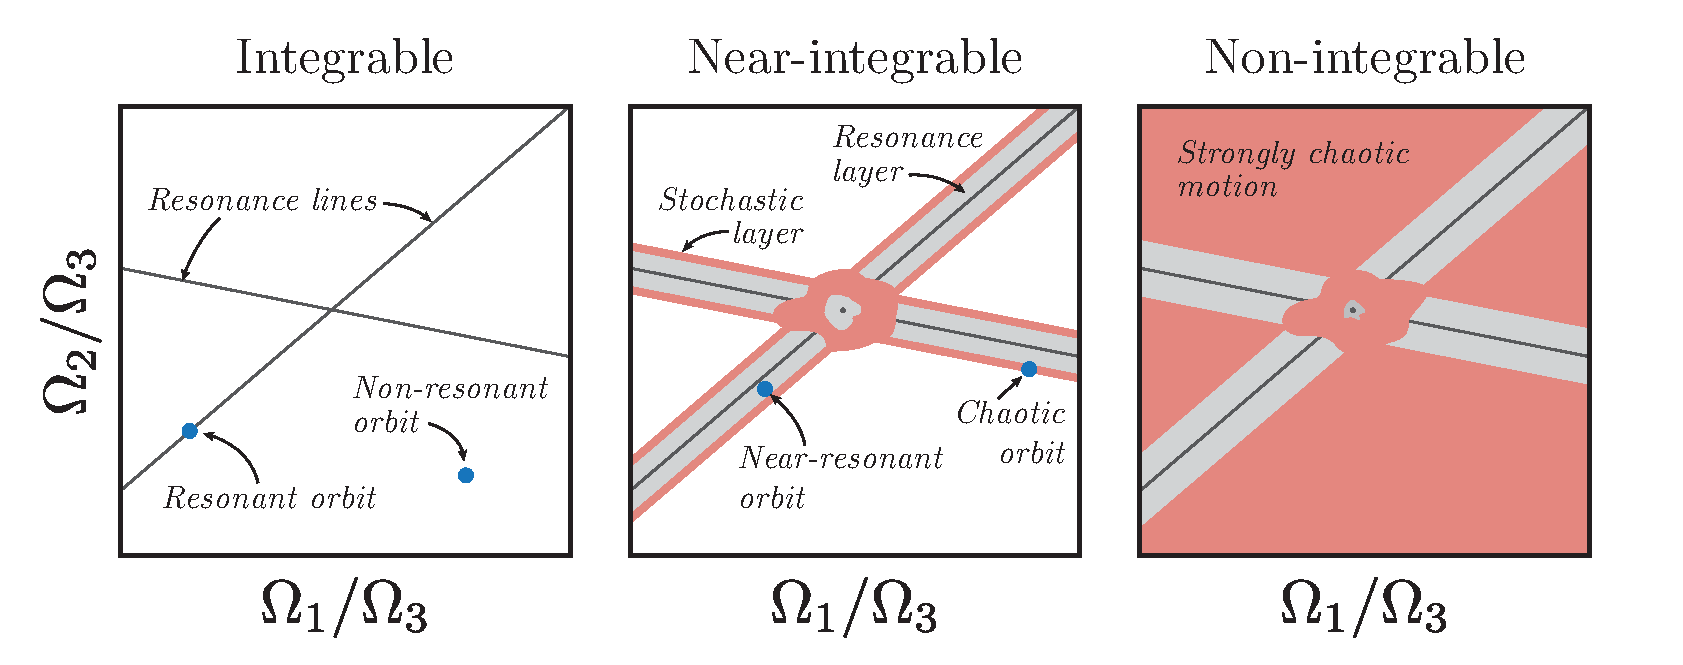
\includegraphics[width=\textwidth]{figures/ch3/cartoons.pdf}
\caption{An illustrative demonstration of the orbit structure for integrable
(left), near-integrable (middle), and non-integrable (right) potentials in terms
of the ratios of the fundamental frequencies. In an integrable potential, only
resonant and non-resonant orbits exist, and all orbits are regular (resonances
appear as lines in frequency-ratio-space). If the potential is perturbed mildly,
resonance layers form around the resonances that host near-resonant orbits which
behave like resonant orbits but have an additional frequency corresponding to
libration about the resonance. Where resonances overlap or near separatrices,
stochastic layers form and orbits will be chaotic. For more strongly perturbed
potentials, many of the non-resonant orbits may become chaotic but resonance
layers may grow and still remain regular. }
\label{fig:cartoons}
\end{center}
\end{figure}

\subsection{Orbits in near- and non-integrable potentials}

The orbit structure of near-integrable potentials can be understood by
considering a Hamiltonian that is a small perturbation away from being globally
integrable---that is, a Hamiltonian that may be written
\begin{equation}
	H(\boldsymbol{J}, \boldsymbol{\theta}) = H_0(\boldsymbol{J}) + \epsilon \, H_1(\boldsymbol{J}, \boldsymbol{\theta})
\end{equation}
where $H_0(\bs{J})$ represents an integrable Hamiltonian, and $\epsilon$ is a
small parameter that determines the perturbation strength \citep[a description
of perturbation theory applied to nonlinear Hamiltonians is given
in][]{lichtenberg83}. When $0 < |\epsilon| \ll 1$, resonant surfaces become
`thick' resonant layers, within which orbits are qualitatively similar to the
parent resonant orbit \citep[e.g.,][]{merritt99}. These resonant layers are then
generically surrounded by stochastic layers where chaotic motion occurs (in the
vicinity of separatrices). Chaotic orbits are not bound to the surface of a
torus and instead fill a (2N-1)-dimensional volume where a continuous set of
tori would exist in an unperturbed Hamiltonian, $H_0$. While the frequency
spectrum of sub-sections of a regular orbit are indistinguishable (i.e. measured
over a finite interval of time), the frequency spectra of sub-sections of a
chaotic orbit will evolve stochastically.

Figure~\ref{fig:cartoons} (middle panel) shows a cartoon of frequency space for
a near-integrable potential (a small perturbation away from the potential in the
left panel) assuming the resonances are stable. Much of the structure that was
present in the integrable potential remains in the near-integrable case, but the
differences are highlighted. Orbits in the resonant layers surrounding the
resonances (grey) are near-resonant orbits that librate around the resonance and
have finite thickness \citep[e.g.,][]{merritt99}. Chaotic orbits in the
stochastic layer (red) behave erratically depending on the surrounding resonance
structure. If the stochastic layer is small and the chaotic orbit is therefore
confined, the orbit may behave nearly regular for long periods of time. If the
resonance in the unperturbed Hamiltonian is unstable, all orbits associated with
the resonance will be chaotic; unstable resonances form linear gaps in
frequency-space (this is not shown in the cartoon but are seen in
Figure~\ref{fig:logfreqs}). Thus, only some resonances in the perturbed system
will retain the signature of a resonance.

For small values of $\epsilon$, many regular orbits survive and only small
chaotic regions are introduced, especially in the vicinity of the intersection
of two resonance lines \citep[commonly referred to as `resonance overlap';
see][]{chirikov60}. As the strength of the perturbation increases, eventually
most tori associated with non-resonant motion will be destroyed.
Figure~\ref{fig:cartoons} (right panel) qualitatively shows this
phenomenon---the resonant and resonant-layer orbits may still be regular, but
many or all of the non-resonant orbits will be chaotic. As the perturbation
strength increases, eventually the uni- and bi-resonant tori are also
destroyed---these are less susceptible to destruction from perturbations
\cite[for a more quantitative illustration of this transition from integrability
to global chaos, see Figure~9 in][]{valluri98}.

When $\epsilon$ is large, there is no general prediction for the resulting
behavior, however it seems that more complicated and physically motivated
triaxial potential models for galaxies follow the intuition gained from the
small-perturbation picture described above, at least for certain parameter
choices \citep[e.g.,][]{valluri98, merritt99}. We therefore expect a large
number of regular orbits will survive---the so-called Kolmogorov–Arnold–Moser
(KAM) tori---however the tori that survive will be separated by regions of
chaotic motion. Any transformations to angle-action coordinates must be defined
local to each resonance region due to the destruction of tori and chaotic motion
which lead to discontinuous changes in orbital properties.

\subsection{The behavior of chaotic orbits in non-integrable potentials}\label{sec:ch4-behavior-chaotic}

Chaotic orbits have no orbital actions and only conserve energy (if the
potential is time-independent). The orbits therefore do not have a single set of
fundamental frequencies, but rather the frequencies that describe the character
of motion evolve with time. In near-integrable potentials, the frequencies of
consecutive sub-sections of a chaotic orbit diffuse both around resonance
layers\footnote{Note that during this diffusion, the frequencies never exactly
hit those of a KAM torus but evolve stochastically around these discrete, stable
tori \citep[cf. Figure 2 in][]{laskar99}. (a sort of stochastic libration) and
along the stochastic layers that surround the resonances (Arnold diffusion).}
For weakly chaotic orbits, motion around a resonance layer can occur with a
frequency close to the libration frequency of the nearby stable orbits in the
resonance layer. Thus, if the resonance libration frequency is small, motion
around a resonance can modulate the frequency spectrum of an orbit over an
orbital time. However, the stochastic layers are often bounded in the direction
orthogonal to the resonance by other stable, resonant regions so that the
frequencies or actions can not change by large factors (unless there are other
nearby resonances and overlapping stochastic layers, in which case the motion
may be strongly chaotic).

The rate of diffusion along stochastic layers via Arnold diffusion depends on
the local resonant structure and is hard to predict. This has been done
analytically for simple potentials \citep[e.g.,][]{chirikov79}. For systems with
$N>2$ dof, the stochastic layers connect and form an intricate network of
stochasticity known as the Arnold web; an orbit that ergodically mixes over its
energy hypersurface must traverse this web, though the timescales typical for
this phenomenon are many thousands of orbital periods.

Arnold diffusion is not expected to be significant for most orbits over
timescales relevant to galaxies (10s of orbits), however chaotic motion across
resonances can occur over short times. If a stochastic trajectory is surrounded
by regular orbits, it may be trapped around a regular parent orbit for long
periods of time before escaping to another such semi-bounded region where it can
become trapped around another parent orbit (a process by which it may eventually
explore the whole Arnold web)---such orbits are commonly referred to as `sticky
orbits.' Additionally, if the volume of the surrounded region in frequency space
is comparable to the characteristic spread of frequencies in the tidal debris,
this small-scale evolution will be important for tidal debris.

\subsection{Mixing of orbit ensembles}\label{sec:ch4-chaotic-mixing}

An ensemble of regular orbits (e.g., tidal debris) will phase-mix because of
(small) differences in the fundamental frequencies of the orbits. The frequency
distributions of thin streams are generally close to one-dimensional---that is,
one eigenvalue of the distribution of frequencies for an orbit ensemble will be
much larger than the others because of the local shape of the Hessian of the
potential \citep{helmi99, sanders13a, bovy14}. Phase-mixing generically leads to
power-law decay of the mean density of the ensembles: initially, the density
decreases linearly in time because of the large, nearly one-dimensional spread
in frequencies, then may proceed as $t^{-2}$ to $t^{-3}$ depending on relative
sizes of the other eigenvalues of the frequency-space distribution
\citep[e.g.,][]{helmi99, vogelsberger08}.

Generically, a small ensemble of chaotic orbits will lose coherence much faster
than for regular orbits \cite[see, e.g.,][]{kandrup94, merritt96, kandrup03},
however this depends on the details of the resonant structure around the
ensemble and the chaotic evolution of the individual orbits and is thus
difficult to predict. For example, ensembles of orbits `stuck' between
resonances may quickly spread to fill the allowed volume, but then the orbits
must escape this confinement and diffuse through the Arnold web to reach a fully
mixed state \citep{merritt96}. That is, while the orbit is stuck, the
small-scale variations effectively cause an increase in the variance of the
frequency distribution, which would enhance mixing of the debris in
configuration-space. In this work, we investigate the consequences of short-time
but small-scale frequency evolution and hypothesize that this may explain the
enhanced density evolution of tidal debris around weakly chaotic regions where
chaotic timescales are predicted to be long \citep[e.g.,][]{pearson15}. We then
discuss how this would affect our understanding of the coherence and density
evolution of tidal streams.

\section{Numerical methods}\label{sec:ch4-methods}

Our goal is to map the orbit structure of arbitrary (galactic) potentials, with
an emphasis on identifying the chaotic orbits and understanding the evolution of
these ensembles of orbits over short times. In particular, we aim to understand
how this chaos-enhanced density evolution can affect tidal stream morphology. In
this section, we describe the methods we will use to detect and quantify the
strength of chaos for large grids of orbits.

\subsection{Potential choice}\label{sec:ch4-potential}

The density distributions within dark-matter haloes formed in cosmological
$N$-body simulations are generically triaxial \citep[e.g.,][]{jing02, bett07,
zemp09, veraciro11}. With the inclusion of baryonic physics and sub-grid
prescriptions for energy input due to supernovae and other feedback mechanisms,
the inner potential ($\lesssim$$0.1R_{\rm vir}$ for a $\approx$$10^{12}~\msun$
halo mass) typically becomes more spherical, though the magnitude of this
reshaping depends on the particular merger history and star formation efficiency
within a given halo and the mass and shape of the baryonic component
\citep[e.g.,][though in Milky Way-like galaxies, baryonic disks will add
non-sphericity to the total potential]{dubinski94,kazantzidis04, debattista08,
bryan13, butsky15}. It is less clear what happens to the outer halo
\citep[e.g.,][]{zemp11, valluri13}.

\citet[][hereafter JS02]{jing02} found that a triaxial generalization of the NFW
density profile \citep{navarro96} generates excellent fits to the density
distributions within haloes in their high-resolution (dark-matter-only) $N$-body
simulations, and they provide probability distributions for the axis ratios of a
large sample of these haloes. JS02 find median axis ratios of $c/a \approx 0.55$
and $b/a \approx 0.77$ where $a$ is the major axis, $b$ the intermediate, and
$c$ the minor axis.\footnote{Note that JS02 use the opposite notation so that
$c$ is the major and $a$ is the minor axis.} These are largely consistent with
findings from more recent simulations \citep[e.g.,][]{bett07, veraciro11,
butsky15, zhu15} and consistent with constraints from weak lensing that place a
lower limit on minor-to-major axis ratios of $c/a\gtrsim0.5$
\citep{vanuitert12}. JS02 find significant scatter in the distributions of
concentration parameter, $c_e$, or scale radius (depending on choice of
parametrization).

All of these parameters are specified in terms of the \emph{density}; for orbit
analysis, we need to determine the form of the potential in terms of these
parameters, which, in general, requires numerical integration of the density at
each position of interest. For computational efficiency, many authors instead
express the triaxiality in the form of the potential, but this can lead to
unphysical situations where the density becomes negative. \citet{leesuto03}
derive a perturbative expansion of the potential integral for a triaxial NFW
density and show that the expansion is accurate even for modest axis ratios
(e.g., the median values shown above).

\begin{figure}[h]
\centering
    \subfloat{
      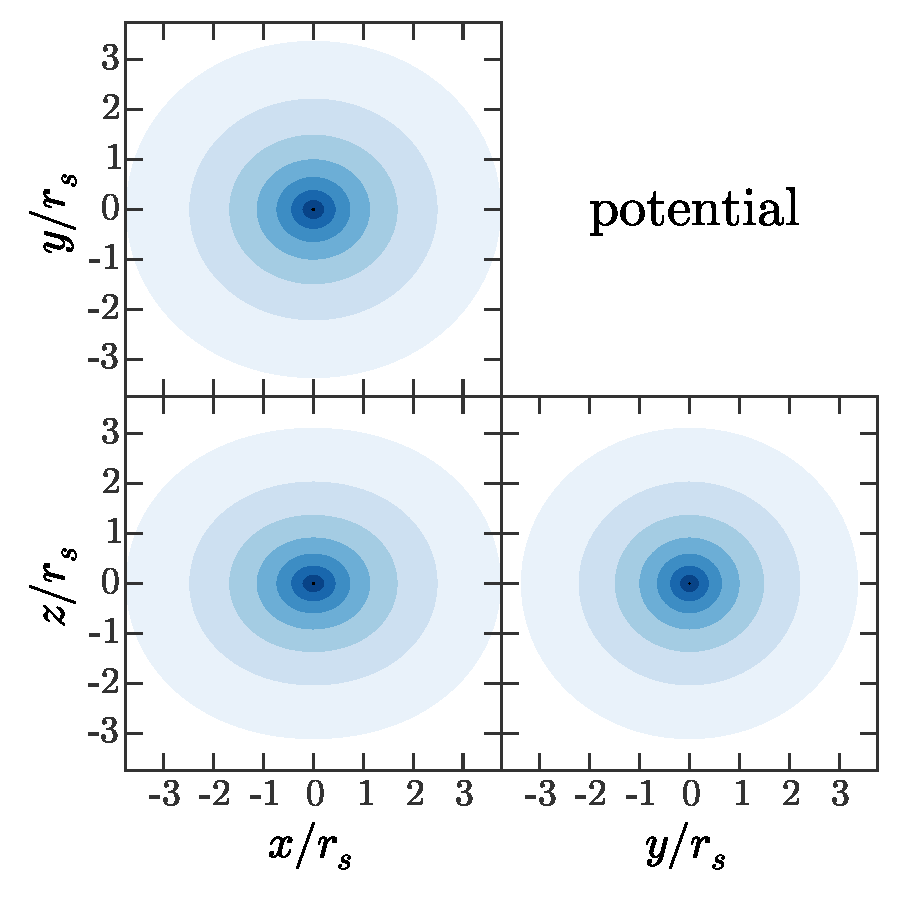
\includegraphics[width=0.45\textwidth]{figures/ch3/potential.pdf}
    }
    \subfloat{
      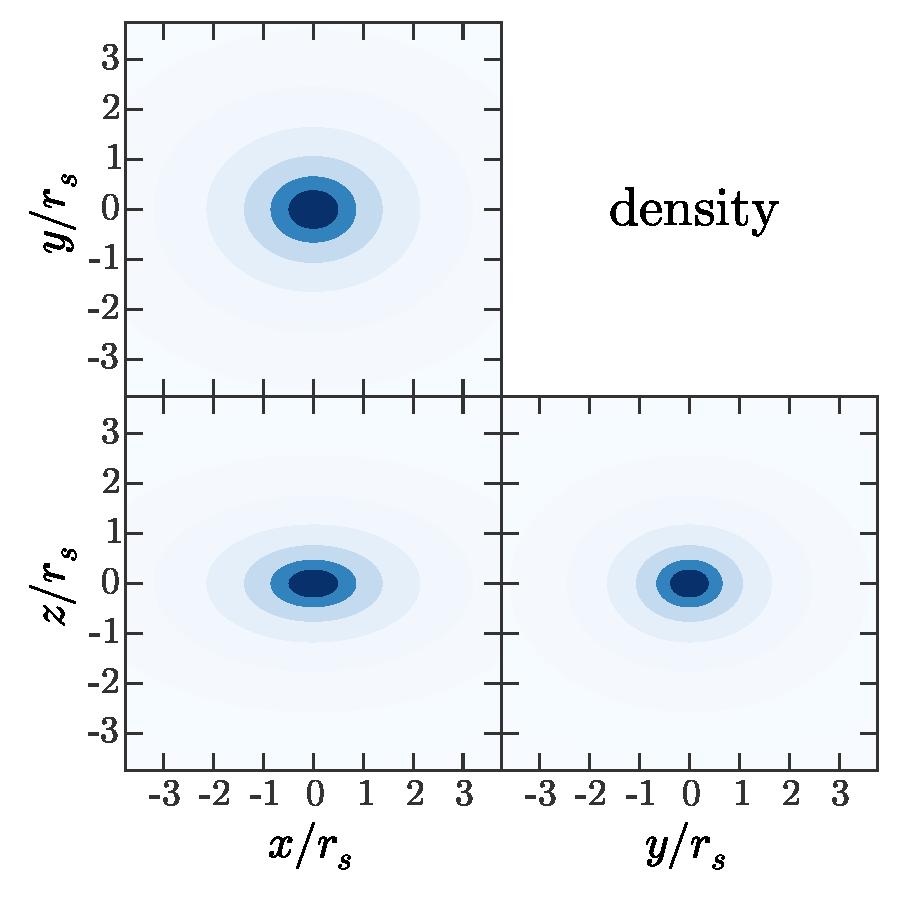
\includegraphics[width=0.45\textwidth]{figures/ch3/density-contours.pdf}
    }
\caption{Equipotential contours (left) and isodensity contours (right) for the
triaxial NFW potential considered in this work. For the potential plot there are
eight contour levels evenly spaced and linear in the value of the potential. For
the density plot there are eight contour levels logarithmically spaced from
$10^4~\msun~{\rm kpc}^{-3}$ to $10^7~\msun~{\rm kpc}^{-3}$.}
\label{fig:ch4-potential}
\end{figure}

In this work, we use the triaxial potential expression from \citet{leesuto03},
parametrized in a slightly different manner. In terms of spherical
coordinates\footnote{$(r,\phi,\theta)$ = (radius, azimuth, colatitude)} with the
radius normalized by the scale radius, $u = r/r_s$
\begin{align}
	\Phi(u,\phi,\theta) &\approx \frac{v_c^2}{A}\left[F_1(u) + \frac{1}{2}(e_b^2 + e_c^2)F_2(u) + \frac{1}{2} [(e_b\sin\theta \sin\phi)^2 + (e_c\cos\theta)^2] F_3(u) \right]\label{eq:potential}\\
	A &= \left(\ln2 - \frac{1}{2}\right) + \left(\ln2-\frac{3}{4}\right) (e_b^2 + e_c^2)
\end{align}
where $e_b = \sqrt{1 - (b/a)^2}$, $e_c = \sqrt{1 - (c/a)^2}$, and $v_c$ is the
circular velocity at the scale radius, $r_s$, for the spherical case. The
functions $F_i(u)$ are given in the appendix of \cite{leesuto03}. We chose
$r_s=20~{\rm kpc}$ and $v_c = 175~{\rm km}~{\rm s}^{-1}$ by taking the mean halo
concentration for a ${\rm M}_{vir} \approx 10^{12}~\msun$ halo, $c_e\approx5$,
from \cite{jing02} and by assuming $R_{vir}\approx200~{\rm kpc}$.
Figure~\ref{fig:ch4-potential} shows equipotential contours of this potential, and
Table~\ref{tbl:potential} summarizes the potential parameters.

\begin{table*}[ht]
\begin{center}
	\begin{tabular}{ c  c }
	         Parameter & Value\\\toprule
		$v_c$ & 175~km~s$^{-1}$\\
		$r_s$ & 20~kpc\\
		$a$ & 1\\
		$b$ & 0.77\\
		$c$ & 0.55\\
		\midrule
		$T_{abc}$ & 0.58\\
		\bottomrule
		\end{tabular}
    \caption{Summary of parameters for the triaxial NFW potential
    (Equation~\ref{eq:potential}) used in this work. Triaxiality is introduced
    in the density (rather than the potential) to ensure that the density is
    physical at all radii. Velocity scale, scale radius, and axis ratios are
    chosen to match the median halo parameters for a $M_{\rm vir} \approx
    10^{12}~\msun$ halo from \citep{jing02}. The triaxiality parameter, $T_{abc}
    = \frac{a^2 - b^2}{a^2 - c^2}$, is also given. \label{tbl:potential}}
\end{center}
\end{table*}

This potential is a simple (and unrealistic) model for the total potential of a
Milky-Way-like galaxy, however it represents a conservative choice for exploring
the structure of orbits in the haloes of such galaxies. Realistic galactic
potentials will have a significant component due to the disk and bulge, radially
changing axis ratios or orientations \citep[e.g.,][]{romanowsky98,
kazantzidis04,debattista08,veraciro11,butsky15}, significant substructure
\citep{moore98,zemp09}, or time dependence \citep[either from bulk rotation,
mass growth, mergers, etc.; see, e.g.,][]{bailin05}. We expect inclusion of any
of these effects to increase the complexity of the resonant structure and
influence of chaos (see Section~\ref{sec:ch4-discussion}).

\subsection{Orbit integration}\label{sec:ch4-integration}

We use the Dormand-Prince 8th-order Runge-Kutta scheme \citep{prince81} to
integrate orbits in the above potential. Specifically, we use a \texttt{Python}
wrapper over the \texttt{C} implementation by \cite{hairer93}. For all orbits we
ensure that energy is conserved to $|\Delta E/E_0| \leq 10^{-8}$ by the end of
integration, however most orbits conserve energy to a part in
$\approx$$10^{-13}$. Unless otherwise specified the integration timesteps are
chosen so that there are 512 steps per strongest orbital period component, but
the integrator uses adaptive stepping between each main step in order to satisfy
a specified tolerance (we set the absolute tolerance to $\approx$100 times
machine precision, $\texttt{atol} = 10^{-13}$).

\subsection{Lyapunov exponents} \label{sec:ch4-lyap}

The most well-known method for assessing chaotic motion is to analyze the
Lyapunov spectrum or maximum Lyapunov exponent (MLE) of an orbit
\citep{lyapunov92}. The MLE measures the mean rate of divergence of two
infinitesimally separated orbits and is only strictly defined in terms of a
limit that goes to infinite time. Thus, we can never truly compute the MLE and
it can take integration for many thousands of orbital periods to compute a
converged numerical approximation of the MLE for a moderately chaotic orbit. In
this work, we use the algorithm introduced by \cite{wolf85} for computing the
MLE (for more a more detailed description of this algorithm, see
Appendix~\ref{sec:ch4-lyapapdx}).

The MLE, $\lambda_{\rm max}$, is interpreted as a rate that quantifies the
exponential divergence of infinitesimally close chaotic orbits. It is therefore
useful to consider the corresponding $e$-folding time by inverting the rate,
\begin{equation}
	t_{\rm \lambda} = \frac{1}{\lambda_{\rm max}}.
\end{equation}
We will use this as the prediction from the Lyapunov exponent for the timescale
over which chaos should be dynamically important for a given orbit.

\subsection{Frequency diffusion rate}\label{sec:ch4-naff}

Bounded, regular orbits in a triaxial potential have three fundamental
frequencies, $\bs{\Omega}$, that determine the periodic behavior of motion. The
motion in any canonical coordinate can therefore be decomposed as a Fourier sum
(Equation~\ref{eq:fourier}) where the Fourier frequencies are linear, integer
combinations of the fundamental frequencies (Equation~\ref{eq:fourierfreq}).
\cite{laskar93} introduced a method for recovering the fundamental frequencies
of an orbit that effectively uses fast-Fourier transforms (FFTs) of complex
combinations of the motion (e.g., $x(t) + i v_x(t)$) to identify the
frequencies. This method is referred to as `Numerical Approximation of
Fundamental Frequencies' (NAFF) and has been used extensively in planetary
dynamics \citep[e.g.,][]{laskar93b, laskar96} and galaxy dynamics
\citep{papaphilippou98, valluri98}, especially in the study of orbits in
triaxial systems. We have implemented and tested a version of this procedure in
the \project{Python} programming language. Our implementation differs slightly
from the original definition and from that used in \cite{valluri98}; we refer to
this slight modification of the algorithm as \superfreq\ \citep{superfreq} and
the code is open-source and publicly available on
\project{GitHub}.\footnote{\url{https://github.com/adrn/SuperFreq}} For more
details about the algorithm and differences with previous work, see
\cite{laskar88, laskar93, papaphilippou96} and Appendix~\ref{sec:ch4-naffapdx}.

If an orbit is chaotic, the motion can no longer be expanded in terms of a
single set of fundamental frequencies. For a weakly chaotic orbit, the orbit may
appear consistently periodic over long windows of time. \superfreq\ will pick
out a set of frequencies for chaotic orbits that correspond to the largest peaks
in the power spectrum of the orbits, however these peaks will change location
and amplitude with time. For more strongly chaotic orbits, the power spectrum
will be quite noisy and the peak frequencies may change erratically when
comparing two consecutive sections of orbit. The frequencies picked out by
\superfreq\ for such orbits will therefore represent the average periodic nature
of the orbit over a given integration window. Following previous work, we define
the fractional frequency diffusion rate, $\mathcal{R}$, in the $k$th fundamental
frequency as
\begin{equation}
	\mathcal{R}_k = \frac{\Omega_{k}^{(2)} - \Omega_{k}^{(1)}}{\Omega_{k}^{(1)} \, \Delta t} \label{eq:fdrate}
\end{equation}
where the upper index refers to the two consecutive sections of orbit and
$\Delta t$ is the length of each integration window \citep{laskar93, valluri98,
valluri12}. By inverting this rate, we can compute the timescale over which we
expect order-unity changes to the fundamental frequencies: the \emph{frequency
diffusion time} is defined as
\begin{equation}
	t_\Omega = \, (\max_{a_k} \, \mathcal{R}_k)^{-1} \label{eq:fdtime}
\end{equation}
where the maximum is taken with respect to the corresponding amplitudes, $a_k$,
of the fundamental frequency components \citep[see][]{valluri12}.

For a small ensemble of orbits (e.g., tidal debris), a more relevant timescale
is the time over which the change in frequencies for a single orbit is
comparable to the spread of frequencies in the ensemble. We can estimate this
timescale by multiplying the frequency diffusion time by a factor equal to the
fractional spread in frequencies of the debris. For example, a globular cluster
typically has $\approx$0.1\% spreads in fundamental frequencies, so by
multiplying the frequency diffusion time by $f = 10^{-3}$, we can estimate the
time (in number of orbital periods) over which we expect the frequencies to
evolve by this amount.

% =====================================================================
%	Results
%
\section{Results}

In Section~\ref{sec:ch4-results1}, we generate grids of orbits in the potential
described above to map the orbital structure of the potential. We classify each
orbit in terms of the strength of chaos along the orbit as computed using the
Lyapnov and frequency diffusion times of Section~\ref{sec:ch4-methods}. With this
initial classification, in Section~\ref{sec:ch4-results2} we follow the evolution of
ensembles of trajectories generated around each orbit in the initial grid. We
find that the configuration-space density of ensembles around weakly chaotic
orbits evolve faster (e.g., in mean density) than expected given the timescales
over which chaos is computed to be relevant for the parent orbits. In
Section~\ref{sec:ch4-results3}, we explain this phenomenon in the context of how
chaotic diffusion occurs (e.g., Section~\ref{sec:ch4-behavior-chaotic}).

\subsection{Part I: Lyapunov and frequency diffusion times}\label{sec:ch4-results1}

We generate an isoenergy grid of initial conditions along the $xz$ ($y=0$)
plane\footnote{$x$ is the major and $z$ the minor axis.} with energy (per unit
mass), $E$, chosen to span a range of distances comparable to the scale radius
of the potential ($E=-(397.2~{\rm km~s}^{-1})^2$ in physical units; see
Table~\ref{tbl:potential}). We fix $v_x = v_z = 0$, and compute $v_y$ from the
energy. This grid generates all of the major orbit classes (short-axis tubes,
inner long-axis tubes, outer long-axis tubes, stochastic intermediate-axis, and
box orbits). The most numerous orbits in this grid are the short-axis and
long-axis tubes that circulate about either the minor or major axis. Thin tidal
streams may preferentially form along tube orbits rather than box orbits because
of the faster disruption and debris diffusion expected for stellar systems on
radially plunging orbits. Figure~\ref{fig:apoper} shows the grid of initial
conditions in the $xz$ plane---each pixel in this grid represents an orbit, and
the pixels are colored by the median pericentric distance (left) and median
apocentric distance (right) over an integration time of 64 orbital periods. From
here onwards, all lengths are given in units of scale radii, $r_s$, velocities
in units of circular velocity, $v_c$, (see Table~\ref{tbl:potential}) and times
in units of orbital periods, $\periods$.

% Figure ??
\begin{figure}[h]%[p]
\centering
    \subfloat{
      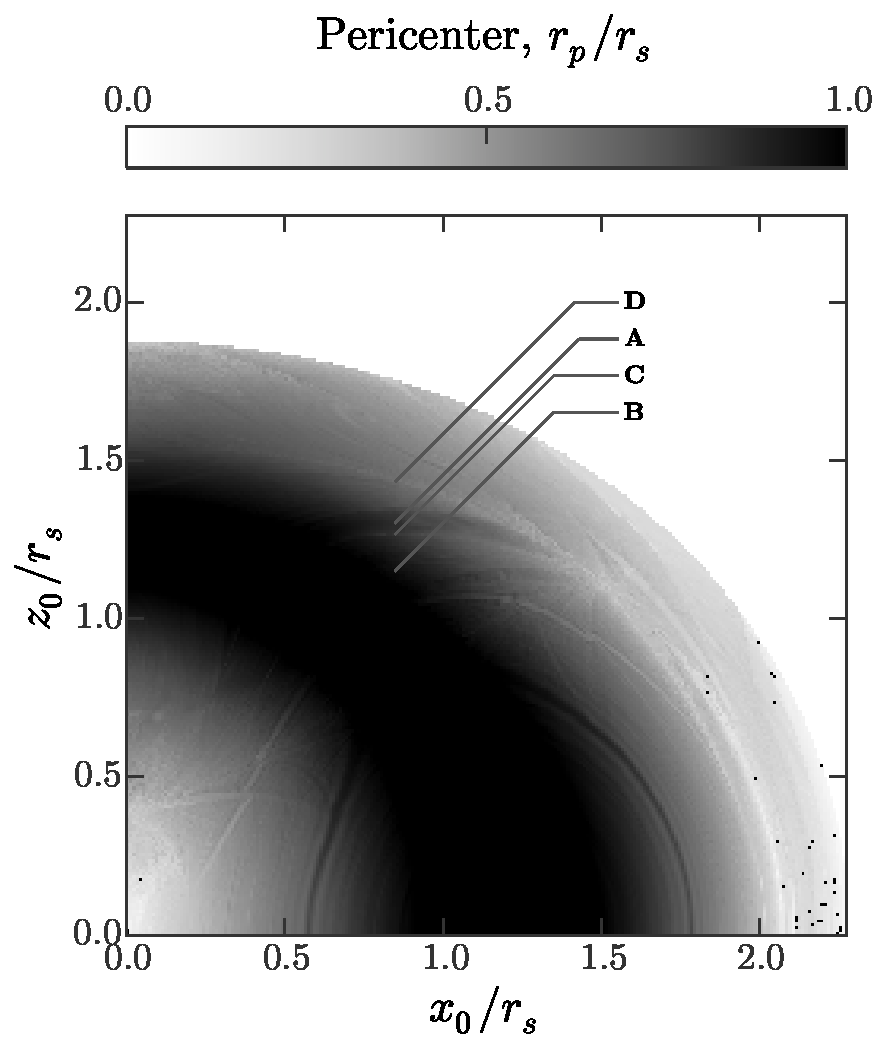
\includegraphics[width=0.45\textwidth]{figures/ch3/pericenter-map.pdf}
    }
    \subfloat{
      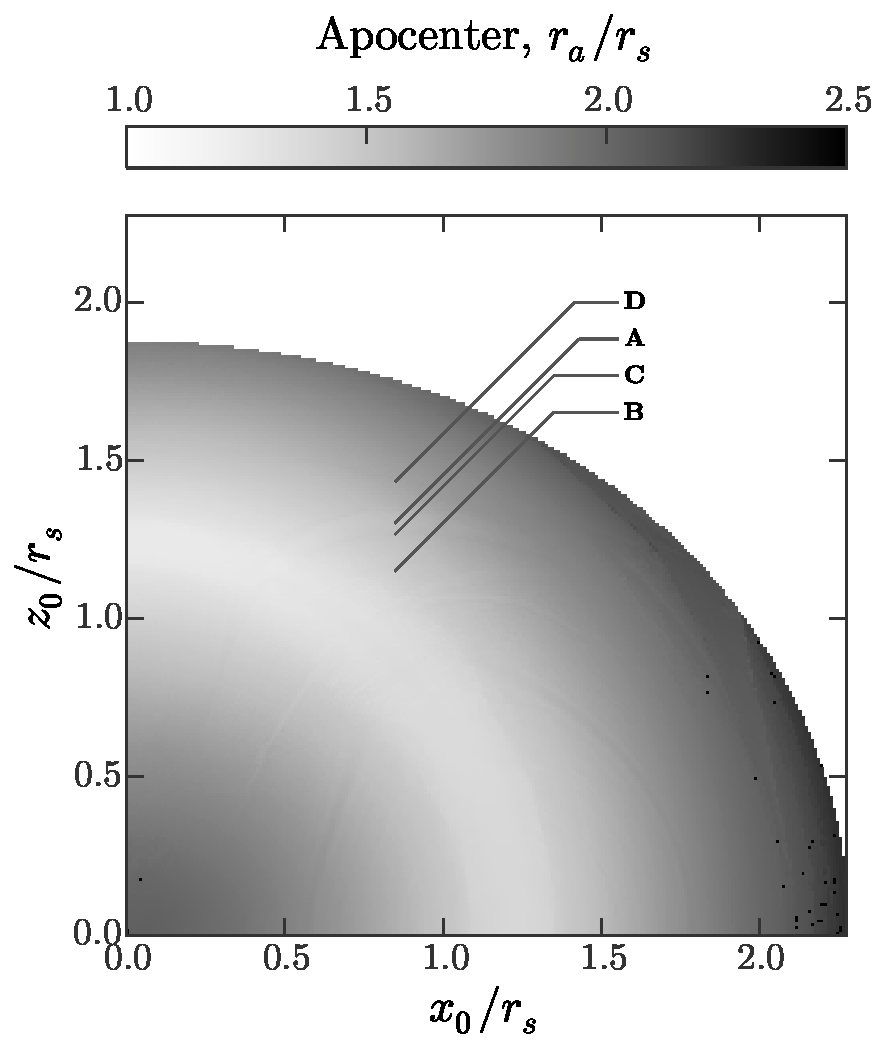
\includegraphics[width=0.45\textwidth]{figures/ch3/apocenter-map.pdf}
    }
\caption{ A grid of isoenergy orbits initialized on the $xz$ plane. All
distances are normalized by the potential scale radius. Each pixel in these
panels represents a single orbit, and the shading of each pixel corresponds to
the median pericentric distance (left) or median apocentric distance (right)
computed over 64 orbital periods. The central black band in the left panel and
white band in the right panel are tube orbits with apocenter-to-pericenter
ratios close to one. The four arrows are explained in Section~\ref{sec:ch4-results2}
and the caption of Figure~\ref{fig:lyapmap}.}
\label{fig:apoper}
\end{figure}

We integrate all orbits in the grid for 10000 orbital periods and use the method
described in Section~\ref{sec:ch4-lyap} to compute the MLEs.
Figure~\ref{fig:lyapmap} again shows the grid of initial conditions, but now the
color corresponds to the logarithm of the inverse of the MLE (the Lyapunov
time). The darker pixels have shorter Lyapunov times and are more chaotic.
Because of the fixed the integration time, the MLE cannot detect weak chaos and
the majority of orbits appear to be regular because they have exceedingly long
Lyapunov times (all white points have $(t_\lambda/\periods) \gtrsim 1000$).

% Figure ??
\begin{figure}[!h]%[p]
\begin{center}
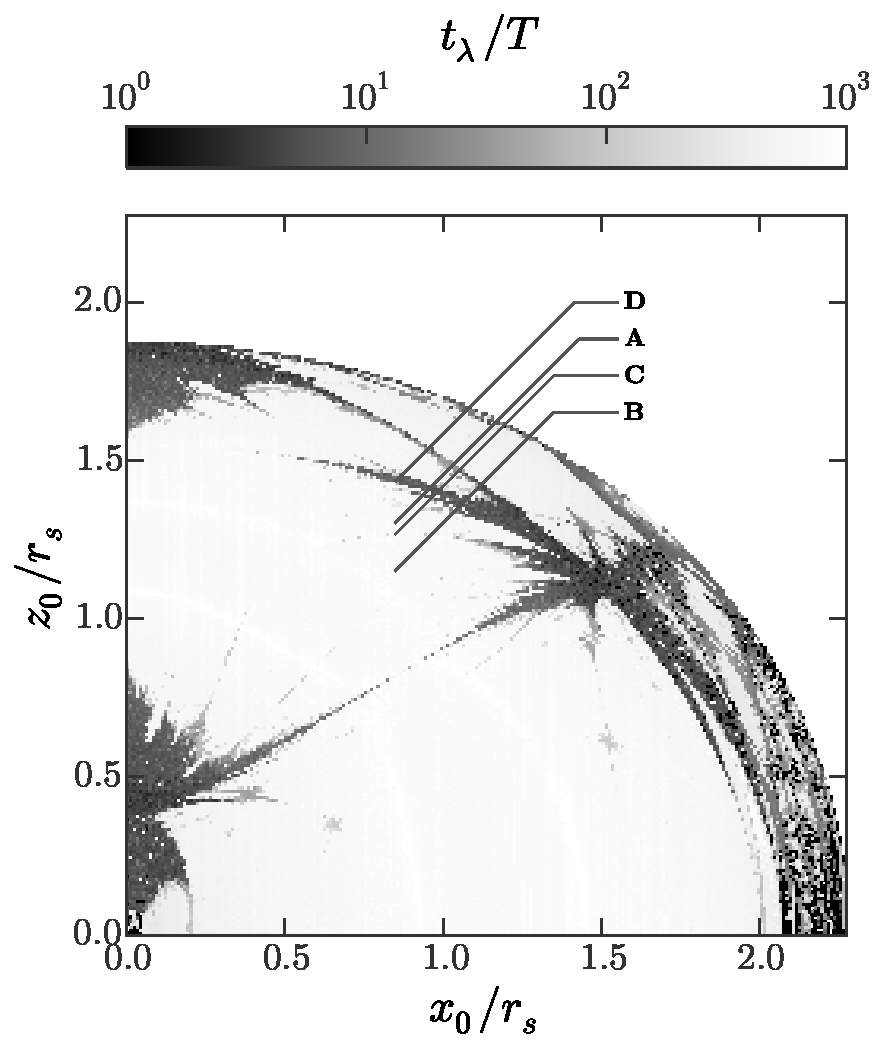
\includegraphics[width=0.8\textwidth, trim={0 0 0 0}]{figures/ch3/lyap_map.pdf}
\caption{ The same grid of orbits as shown in Figure~\ref{fig:apoper}, but now
each pixel is colored by the logarithm of the Lyapunov time (in units of orbital
periods). Orbits are integrated for a total of 10000 orbital periods. Chaotic
orbits with $t_\lambda/\periods \gtrsim 700$ appear regular because the
integration time for each orbit is insufficient to resolve weak chaos. Four
orbits are pointed out with arrows---from top to bottom, these are the strongly
chaotic (D), near-resonant (A), weakly chaotic (C), and non-resonant (B) orbits
of Table~\ref{tbl:orbit-info} (see Section~\ref{sec:ch4-results2}).}
\label{fig:lyapmap}
\end{center}
\end{figure}

For each orbit, we also separately integrate for 256 orbital periods and use
\superfreq\ to compute the fundamental frequencies for the two consecutive
sections of 128 orbital periods. We have chosen this window size so that we
recover the frequencies for regular orbits with fractional error
$\approx10^{-8}$ \citep[we estimate the error in frequency recovery using the
method described in][]{laskar93}. With this integration window we are able to
successfully recover frequencies for $>$99.9\% of the orbits \superfreq.
Figure~\ref{fig:freqdiff} shows the same grid of initial conditions as in
Figure~\ref{fig:lyapmap}, but now the greyscale intensity is set by the
logarithm of the frequency diffusion time. The darker pixels have shorter
frequency diffusion times and are more chaotic. This map reveals the
intersection of this particular energy hypersurface with the rich structure of
resonant surfaces present in this potential and highlights the accuracy of
\superfreq\---weak chaos (grey) is detectable over much shorter integration
periods using frequency analysis, compared to the many tens of thousands of
orbits it would take to detect such features with the maximum Lyapunov exponent.
The tube orbits in this potential are mostly regular or only mildly
chaotic---the largest regular regions are associated with the short-axis and
long-axis tube orbits---however islands of stronger chaos do appear, especially
at the intersections of resonances where resonance overlap occurs.

% Figure ??
\begin{figure}[!h]%[p]
\begin{center}
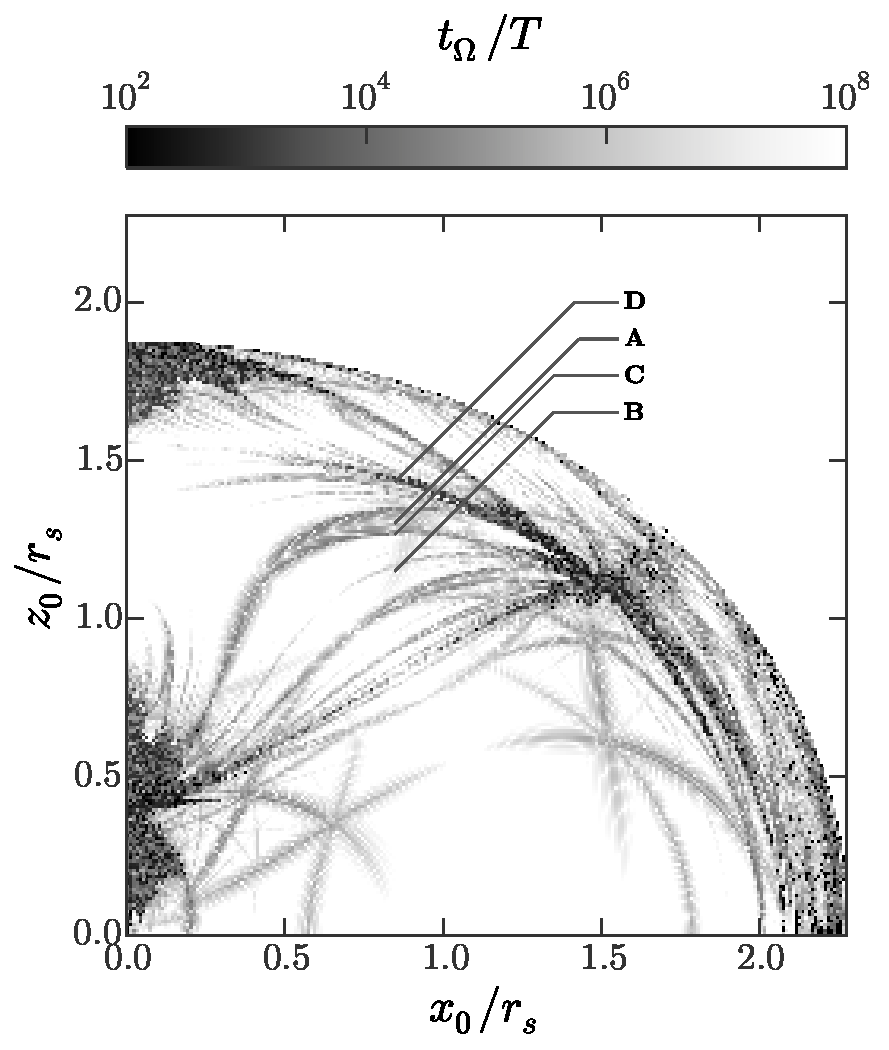
\includegraphics[width=0.8\textwidth, trim={0 0 0 0}]{figures/ch3/fdiff_map.pdf}
\caption{The same grid of orbits as shown in Figure~\ref{fig:apoper}, but now
each pixel is colored by the logarithm of the frequency diffusion time (again in
units of orbital periods). The frequencies are computed in two consecutive
windows, each of which has length equal to 40 orbital periods. The frequencies
are measured precisely so that small changes in the frequencies can be detected
over just $\approx$10s of orbits. Four orbits are pointed out with arrows---from
top to bottom, these are the strongly chaotic (D), near-resonant (A), weakly
chaotic (C), and non-resonant (B) orbits of Table~\ref{tbl:orbit-info} (see
Section~\ref{sec:ch4-results2}).} \label{fig:freqdiff}
\end{center}
\end{figure}

The strongest chaotic regions (black) appear in both of the above grids
(Figure~\ref{fig:lyapmap} and Figure~\ref{fig:freqdiff}). Some of the weakly
chaotic unstable resonances do appear in the Lyapunov time map---for example,
near $(x_0,z_0) / r_s \approx(1.5,0.6)$ and $(x_0,z_0) /r_s \approx(0.6,0.4)$
where there is a slight hint of weak chaos (grey) in Figure~\ref{fig:lyapmap}.
The details of the resonant structure is revealed in the frequency diffusion map
from integrations of just 256 orbital periods. While there is rich structure and
a significant number of weakly chaotic orbits, the majority of the orbits have
estimated chaotic timescales corresponding to thousands of orbital periods and
are thus not expected to be relevant for tidal stream evolution. In the next
section, we analyze the density evolution of finite-volume ensembles of orbits
around each orbit in the above grids in order to compare the effect of ordinary
phase-mixing of tidal debris with potentially enhanced mixing due to chaos. We
then compare the density evolution of the ensembles to the single-orbit chaos
indicators computed in this section.

\subsection{Part II: Ensemble properties and mixing} \label{sec:ch4-results2}

The Lyapunov and frequency diffusion times measure the timescales over which
chaos is relevant for a given orbit---that is, these quantities are measures of
how infinitesimal deviations will diverge on average from some parent orbit, or
of how long it takes for the frequencies of a single orbit to change by some
amount. Tidal debris is disrupted from progenitor systems with finite spreads in
orbital properties (e.g., energy). For a disrupting, globular-cluster-scale
progenitor, the typical energy or frequency-space dispersion of the debris is
0.1--1\% of the progenitor orbital energy \citep[assuming masses of
$10^4$--$10^6$~\msun;][]{johnston98}, but for a dwarf-galaxy-scale progenitor,
the dispersion can be $\sim$10\%. In this section, we ask whether  the Lyapunov
or frequency diffusion time predict the timescale over which a finite
phase-space volume (e.g., tidal debris) stays coherent.

It is computationally intractable to run full $N$-body simulations for the large
grid of orbital initial conditions of the previous section and we therefore take
a simplified approach for studying how finite-volume debris spreads along each
of these orbits. We instead consider small ensembles of particles meant to
represent debris disrupted from a single tidal disruption event. For a given set
of orbital initial conditions---the `parent' orbit---we integrate for 128
orbital periods, find the phase-space position of the minimum pericenter over
this time, initialize a small ensemble of test particle orbits around this
position, and integrate the orbits of all test particles for some integration
time. We are interested in the degree to which chaos enhances the mixing rate of
orbit ensembles and we therefore want to isolate out the effect of ordinary
phase-mixing along regular orbits. We set the physical scale of the ensemble by
the tidal radius in position and the velocity scale in velocity; the initial
spread in fundamental frequencies will scale as $(m/M)^{1/3}$ like the tidal
radius and velocity scale \citep[e.g.,][]{johnston98, apw14}. If
$(\bs{x}_0,\bs{v}_0)$ are a set of initial conditions at pericenter for a parent
orbit, then $\delta x_{k,i}$ and $\delta v_{k,i}$ are the $k$th components
($k=1,2,3$) of the position and velocity deviation vectors for the $i$th
particle and the magnitude of the offsets are assumed to be Normally distributed
away from the parent orbit:
\begin{align}
	\delta x_{k,i} &\sim \mathcal{N}(0, r_{\rm tide}/\sqrt{3})\\
	\delta v_{k,i} &\sim \mathcal{N}(0, \sigma_v/\sqrt{3})\\
	r_{\rm tide} &= \|\bs{x}_0\| \left(\frac{m}{M(<\|\bs{x}_0\|)}\right)^{1/3} \\
	\sigma_v &= \|\bs{v}_0\|\left(\frac{m}{M(<\|\bs{x}_0\|)}\right)^{1/3}
\end{align}
where $M(<r)$ is the mass enclosed of the host potential within radius $r$, $m$
is the mass scale of the `progenitor,' and $\|\cdot \|$ is the Euclidean norm.
We take $m=10^4~\msun$ to represent globular-cluster-like progenitors, and use
the spherically-averaged enclosed mass of the host potential to estimate the
above debris scales. % we have verified this using regular orbits in a logarithmic potential...

We start by considering four particular orbits chosen from the orbit grid of
Section~\ref{sec:ch4-results1}: a regular, near-resonant orbit (A), a regular,
non-resonant orbit (B), a weakly chaotic orbit (C), and a more strongly chaotic
orbit (D). The orbits were chosen to be close on the orbit grid so that their
orbital properties (e.g., apocenter, pericenter) are similar, but have different
frequency diffusion times; all four orbits are long-axis tube orbits.
Figure~\ref{fig:orbits} shows the orbits in projection over an integration
period of 1024 orbital periods. The initial conditions and chaos diagnostics for
each orbit are listed in Table~\ref{tbl:orbit-info}. Figure~\ref{fig:ensembles}
shows final positions of test-particle ensembles initialized around the four
orbits described above and integrated for 64 orbital periods. A thin stream
forms on the near-resonant orbit (left column), a thin---but more
two-dimensional---stream forms on the non-resonant orbit (middle-left), a more
diffuse stream forms on the weakly chaotic orbit with a slightly `fanned'
morphology (middle-right), and a two-dimensional, `fanned' stream on the more
strongly chaotic orbit (right). Given the long Lyapunov and frequency diffusion
times of the weakly chaotic orbit ($t_\lambda/\periods > 900$,
$t_\Omega/\periods \approx 2\times10^5$), it is surprising that the density
evolution of the ensemble on this orbit appears to be more diffuse than the
regular orbit stream.

% Figure ??
\begin{figure}[h]%[p]
\begin{center}
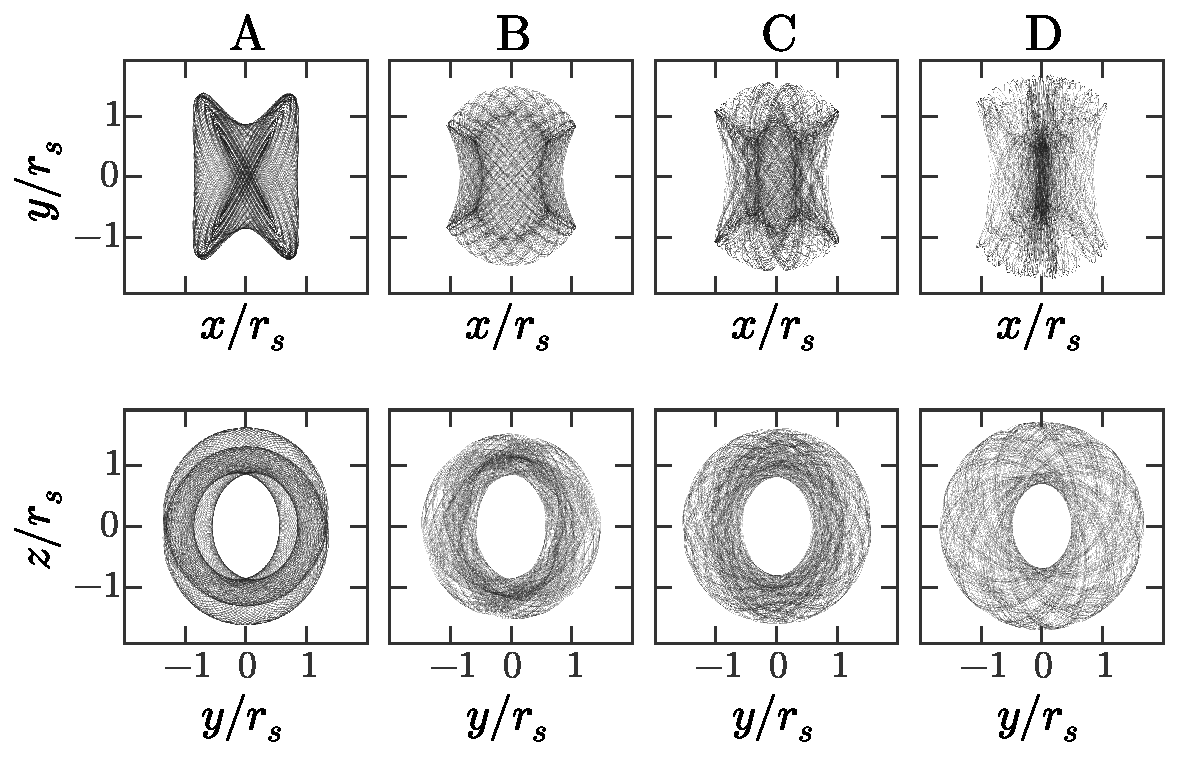
\includegraphics[width=0.8\textwidth]{figures/ch3/four-orbits.pdf}
\caption{Four representative orbits chosen from the orbit grid (e.g.,
Figure~\ref{fig:apoper}): a regular, near-resonant orbit (A), a regular,
non-resonant orbit (B), a weakly chaotic orbit (C), and a more strongly chaotic
orbit (D). All orbits are long-axis tubes with similar pericenters and
apocenters. Orbits in this Figure were integrated for 1024 orbital periods and
are shown in projection.}
\label{fig:orbits}
\end{center}
\end{figure}

% Figure ??
\begin{figure}[h]%[p]
\begin{center}
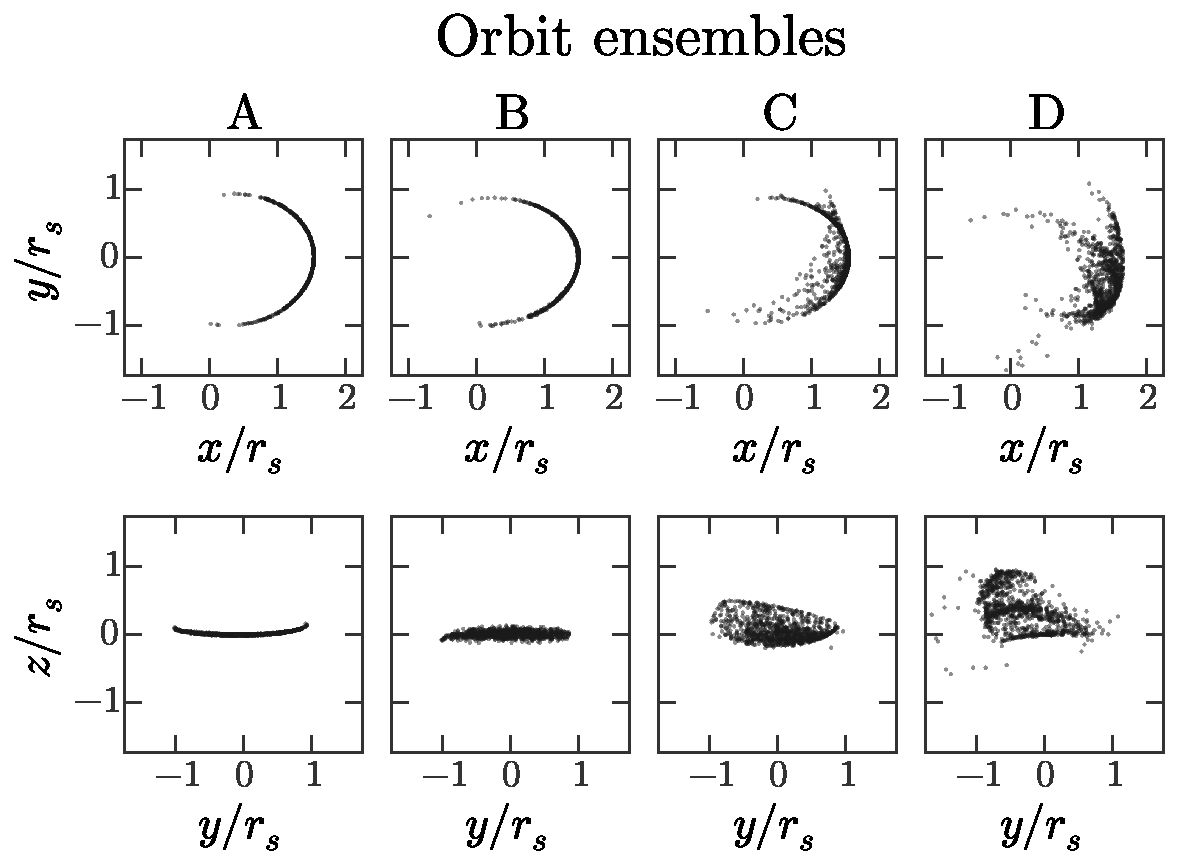
\includegraphics[width=0.8\textwidth]{figures/ch3/ensembles.pdf}
\caption{Final particle positions after integrating unbound,
globular-cluster-sized ensembles of orbits generated around each of the three
$N$-body orbits (Figure~\ref{fig:nbodysims}). The ensembles each contain 1024
particles and are initialized at pericenter. The particle positions
qualitatively match the morphology of the `oldest' debris from the corresponding
$N$-body simulations (Figure~\ref{fig:nbodysims}). }
\label{fig:ensembles}
\end{center}
\end{figure}

We verify that these orbit ensembles capture the nature of more realistic stream
formation by running $N$-body simulations of globular-cluster-mass progenitor
systems on these same four orbits. We use the Self-Consistent Field (SCF) basis
function expansion code \citep{hernquist92} to run the simulations, which we set
up to run from apocenter-to-apocenter (rather than pericenter-to-apocenter as in
the ensembles), but finish with the progenitor in the same location as the
parent orbit in the ensemble evolution described above.
Figure~\ref{fig:nbodysims} shows the final particle distributions rotated so
that the angular momentum of the progenitor orbit is aligned with the $z$-axis.
From a comparison of Figures~\ref{fig:ensembles} and \ref{fig:nbodysims}, it is
clear that the morphology of the ensembles is visually similar to the `oldest'
(first stripped) debris in the $N$-body simulations.

\begin{table*}[ht]
\begin{center}
	\begin{tabular}{c | c c c c c c | c c}
		{\bf ID} & $\bs{x/r_s}$ & $\bs{y/r_s}$ & $\bs{z/r_s}$ & $\bs{v_x/v_c}$ & $\bs{v_y/v_c}$ & $\bs{v_z/v_c}$ & $\bs{t_\lambda/\periods}$ & $\bs{t_\Omega/\periods}$ \\\toprule
A & 0.85 & 0 & 1.303 & 0 & 0.721 & 0 & $>700$ & $>10^7$ \\
\midrule
B & 0.85 & 0 & 1.152 & 0 & 0.849 & 0 & $>700$ & $>10^7$\\
\midrule
C & 0.85 & 0 & 1.27 & 0 & 0.752 & 0 & $>700$ & $\approx 3\times10^5$\\
\midrule
D & 0.85 & 0 & 1.434 & 0 & 0.597 & 0 & 8.14 & $\approx 2.5\times10^4$\\
		\bottomrule
		\end{tabular}
    \caption{Orbital initial conditions from the $xz$ grid for orbits with a
    range of chaotic timescales---A is a regular, near-resonant orbit, B a
    regular, non-resonant orbit, C a weakly chaotic orbit, and D a strongly
    chaotic orbit. Positions ($x$, $y$, $z$) are given in units of scale radii,
    $r_s$, and velocities ($v_x$, $v_y$, $v_z$) in units of scale velocity,
    $v_c$. Chaotic timescales are expressed ($t_\lambda$, $t_\Omega$) in number
    of orbital periods. Recall that the frequency diffusion time, $t_\Omega$, is
    the time over which we expect order-unity changes in the fundamental
    frequencies, hence why the timescales appear quite long.
    \label{tbl:orbit-info}}
\end{center}
\end{table*}

% Figure ??
\begin{figure}[hp!]%[p]
\begin{center}
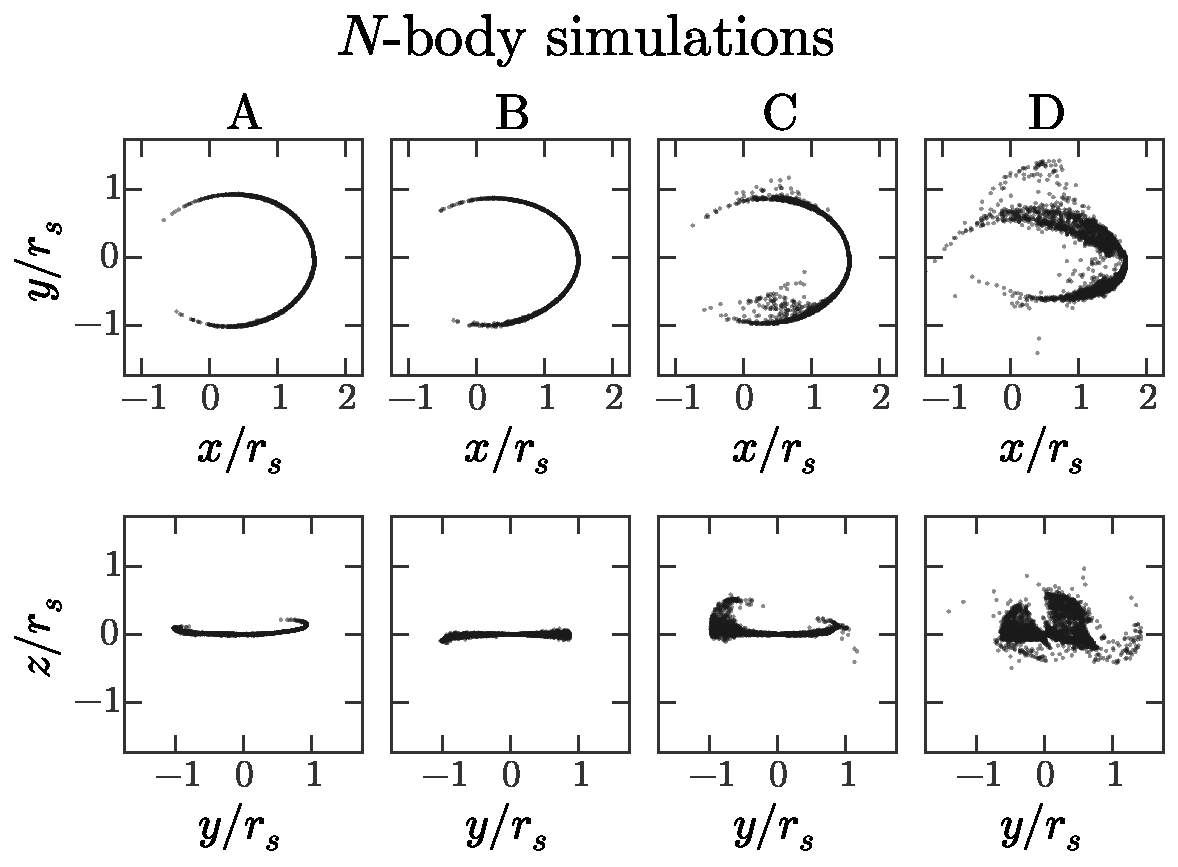
\includegraphics[width=0.8\textwidth]{figures/ch3/nbody.pdf}
\caption{ We use the Self-Consistent Field (SCF) basis function expansion code
\citep{hernquist92} to run $N$-body simulations of globular-cluster-mass
progenitor systems on the three orbits of Figure~\ref{fig:ensembles}. The
progenitor in each simulation is initialized as a $10^4$ particle Plummer sphere
and the background triaxial NFW potential is turned on slowly over 250 Myr to
reduce artificial gravitational shocking. We start the progenitor systems at
apocenter and integrate for $\approx$64 orbital periods so that each simulation
finishes again at subsequent apocenter. The mass of the progenitor is set to
$10^4~\msun$, and the length-scale of the Plummer sphere is set to 5~pc to get
$\approx$50--75\% mass loss over the integration time. Panels show particle
positions from the final snapshots of the simulations---for visualization the
positions have been rotated so that the angular momentum of the progenitor at
the final snapshot are aligned with the $z$-axis. These simulations confirm that
the test-particle orbit ensembles (Figure~\ref{fig:ensembles}) do
(qualitatively) capture the nature of the early-stripped tidal debris. }
\label{fig:nbodysims}
\end{center}
\end{figure}

Visual inspection of Figures~\ref{fig:ensembles} and \ref{fig:nbodysims}
suggests that chaotic mixing of small orbit ensembles affects the
configuration-space evolution of an ensemble over short times, even when the
predicted chaotic timescales (from the Lyapunov and frequency diffusion times)
are long: The mean, single-orbit chaos indicators are not well-suited for
determining the importance of chaotic diffusion on tidal stream evolution. As a
quantitative measure of this enhanced density evolution, we compute the
evolution of the mean configuration-space density for orbit ensembles evolved
around the four parent orbits (A,B,C,D) described above. At each time step, we
use kernel density estimation (KDE)\footnote{We use an implementation from the
Python package \texttt{scikit-learn} \citep{scikitlearn}.} with the ensemble of
particle positions to estimate the configuration-space density field. We use an
Epanechnikov kernel with an adaptive bandwidth: at each evaluation of the
density, we use 10-fold cross-validation to find the optimal kernel bandwidth.
We evaluate the density at the positions of each particle, $\rho_i$, and compare
to the mean initial density, $\mean{\rho_0}$.

Figure~\ref{fig:densities} shows the mean density of the ensemble particles
computed at 256 evenly-spaced intervals from the initial ensemble distribution
to the distribution after 64 orbital periods. Over-laid on each panel are
qualitative power-laws (i.e. not fit to the density evolution) that demonstrate
the expected trends: After initial $t^{-1}$ decay, the mean density of the
near-resonant orbit (A) should follow $t^{-2}$, whereas the non-resonant orbit
(B) will transition from $t^{-2}$ to $t^{-3}$ after long times (and thus
currently display an intermediate power-law index). Given the extremely long
chaotic timescale for the weakly chaotic orbit (C), we would expect the mean
density to follow a simple power-law over long times, however at $\approx$16
orbital periods the density clearly diverges and begins to follow a decaying
exponential. The mean density along the strongly chaotic orbit (D) evolves
stochastically but generally follows a decaying exponential.

Motivated by the noticeable discrepancy between the final mean density between
the two regular (A,B) and the weakly chaotic (C) orbit ensembles---even though
the chaotic timescale of the weakly chaotic ensemble parent orbit is several
times the integration period used above---we compute the final mean density for
orbit ensembles generated around each orbit in the grid described in
Section~\ref{sec:ch4-results1}. For all ensembles, we integrate the orbits for 64
(parent) orbital periods and compute the initial and final values of the mean,
configuration-space density. Figure~\ref{fig:ensemblemap-meandensity} again
shows the grid of initial conditions (Section~\ref{sec:ch4-results1}, but now the
greyscale indicates the ratio of the final mean density to the initial density.
Interestingly, much of the structure that is visible in the upper-half of the
frequency diffusion time map (Figure~\ref{fig:freqdiff}) is again visible in
this map of the density evolution of orbit ensembles. Many features appear as
lighter, curved features in the upper portion of this grid where the density
remains systematically higher---these are the stable resonances of the
potential. Darker regions have systematically lower densities and correspond to
regions of resonance overlap where weakly chaotic orbits are found.

% Figure ??
\begin{figure}[t]%[p]
\begin{center}
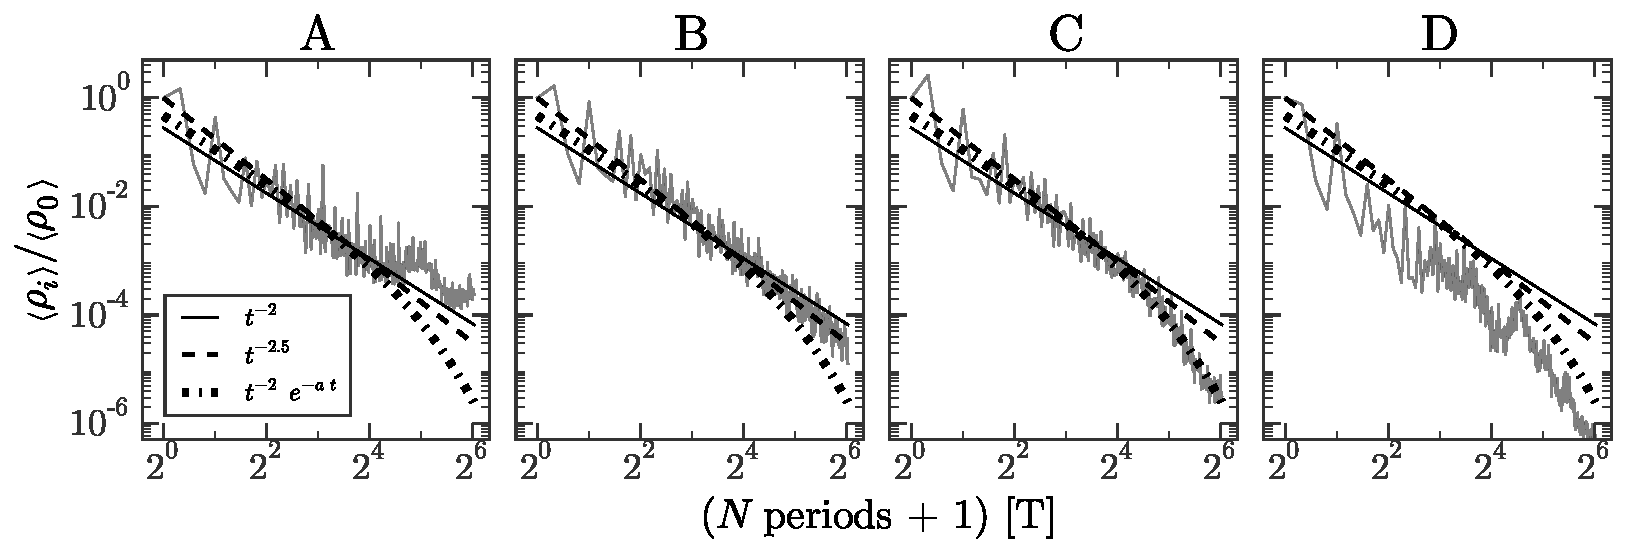
\includegraphics[width=\textwidth]{figures/ch3/ensemble-densities.pdf}
\caption{Evolution of the mean density (normalized by the initial density) of
orbit ensembles around the four orbits (Figure~\ref{fig:orbits}) over 64 orbital
periods. Over-plotted are various power-laws that qualitatively show the decay
of the mean density for the ensembles: the mean density of the near-resonant
orbit (A) follows nearly $t^{-2}$; the non-resonant orbit (B) is slowly
transitioning from $t^{-2}$ to $t^{-3}$; the weakly chaotic orbit (C) initially
follows $t^{-2}$ but then exponential decay takes over; the strongly chaotic
orbit (D) is roughly exponential with fairly erratic density evolution. }
\label{fig:densities}
\end{center}
\end{figure}

However, it is surprising that these features are present: The chaotic
timescales predicted from both the Lyapunov and frequency diffusion times were
typically 100 to 1000s of orbital periods for many of the unstable features
around resonances. The timescales in the lower portion of the grid (where the
orbits are primarily stable, short-axis tube orbits) are simply too long to
detect density differences over 64 orbital periods even from weak chaos in this
particular choice of potential.

It is worth noting that the frequency diffusion time map predicts that the
resonances are surrounded by thick stochastic layers, while in the density map
the resonance layers appear to be stable (and thus lead to higher mean
densities). This comes from a failure of frequency determination: Near
resonances it can take extremely long integration periods to ensure accurate
recovery of the frequencies due to aliasing \citep{laskar03}. However, at the
edges of the resonance layers---where we expect to find stochastic layers and do
see weakly chaotic motion---the frequency diffusion time is a robust indicator
of chaos.

We conclude from these experiments that the degree of chaos is an indicator that
ensembles of orbits may mix faster than predicted from regular phase-mixing,
however the Lyapunov time and frequency diffusion time are not good predictors
for the timescale over which this mixing will occur. To understand this
discrepancy, we next explore why this occurs (Section~\ref{sec:ch4-results3}, in the
context of Section~\ref{sec:ch4-chaotic-mixing}).

% Figure ??
\begin{figure}[hp!]
\begin{center}
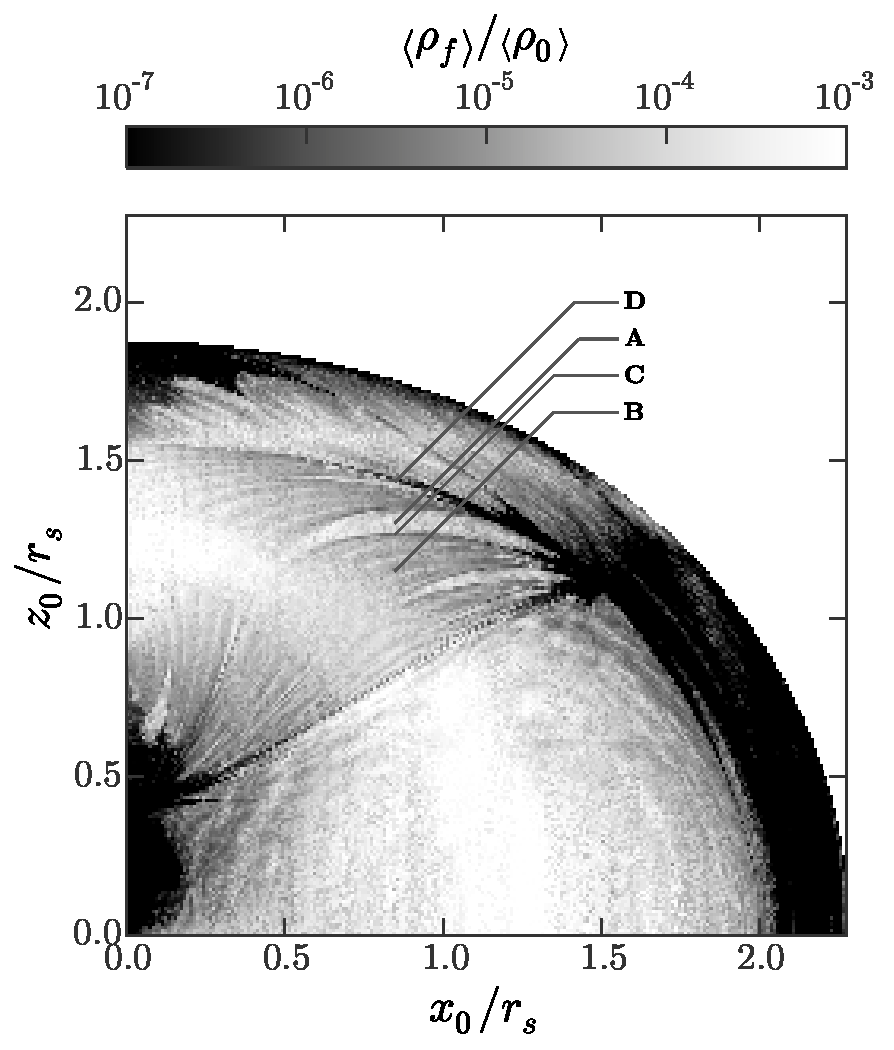
\includegraphics[width=0.8\textwidth, trim={0 0.2cm 0 0}]{figures/ch3/ensemble-map.pdf}
\caption{The same grid of orbits as shown in Figure~\ref{fig:apoper}, but now
the greyscale intensity is set by the mean density of a of small ensembles of
orbits after integration for 64 orbital periods. The orbit ensembles are
generated around each parent orbit in the grid (Section~\ref{sec:ch4-results2}) and
the mean density is a kernel density estimation (KDE) with an adaptive
Epanechnikov kernel. Given the extremely long chaotic timescales of the weakly
chaotic orbits in the upper half of the grid, it is surprising that any of the
high-order resonant structure is visible in this map. Four orbits are pointed
out with arrows---from top to bottom, these are the strongly chaotic (D),
near-resonant (A), weakly chaotic (C), and non-resonant (B) orbits of
Table~\ref{tbl:orbit-info} (see Section~\ref{sec:ch4-results2}).}
\label{fig:ensemblemap-meandensity}
\end{center}
\end{figure}

\subsection{Part III: Short-time frequency evolution}\label{sec:ch4-results3}

Why does chaos manifest itself after just 64 orbital periods around orbits with
predicted chaotic timescales larger than thousands of orbital periods? Both the
Lyapunov exponent and the frequency diffusion rate measure mean, long-term rates
of chaotic diffusion. If a weakly chaotic orbit is confined (by other nearby,
non-overlapping resonances or stable regions), the mean drift of an orbit in
frequency space may be small if computed over timescales long compared to the
orbital time but short compared to the Arnold diffusion time, however
small-scale variation of the frequencies may occur over much shorter timescales.

As a demonstration of the small-scale frequency modulation, we consider again
the four orbits of Section~\ref{sec:ch4-results2} (initial conditions are listed in
Table~\ref{tbl:orbit-info}). To resolve the short-time behavior of the frequency
diffusion (corresponding to motion across or around resonance layers) we compute
the frequencies in a series of rolling windows along each orbit. We use a window
with a width equal to 64 orbital periods and shift the window by an orbital
period between each calculation of the most significant frequencies.
Figure~\ref{fig:four-orbits-freqs} shows plots of the frequencies of each orbit
computed in each window of time---plotted in projection are the percent
deviations of the frequency from the initial value. The difference between the
first window (blue +) and the last window (red x) is 128 orbital periods. For
the two regular orbits, (A) and (B), the frequencies vary only from numerical
issues when recovering the frequencies ($\ll$1\%) and thus the initial and final
value markers overlap. The frequencies of the weakly chaotic orbit (C) evolve
quickly but are bounded to a small volume with fractional size $\approx$1\%
(presumably by nearby resonant surfaces); this is larger than the frequency
spread in globular cluster tidal debris (0.1--0.5\%). The frequencies of the
strongly chaotic orbit (D) also evolve quickly but fill a larger volume.

We see now where the discrepancy between chaotic timescales and the observable
effects of chaos arise in tidal debris: even if the large-scale diffusion of
frequencies is slow, an orbit may explore a region of frequency space over much
shorter times. The frequency diffusion time (Equation~\ref{eq:fdtime}) is an
estimate of the time over which the mean value of the frequencies evolves,
however the \emph{variance} of the frequencies over short times is dynamically
relevant for small ensembles. This small-scale variability is insignificant for
the evolution of global structure in, for example, an elliptical galaxy or in
erasing substructure in the Solar neighborhood \citep[e.g.,][]{maffione15}, but
is signifiant for the morphological evolution of tidal debris with small spreads
in frequencies.

We therefore expect a small ensemble of orbits in frequency space to expand over
short times around even weakly chaotic parent orbits and the debris should
therefore appear dynamically hotter in real-space. The effect is especially
significant if the chaotic evolution of the frequencies occurs orthogonal to the
largest eigenvector of the distribution of frequencies or the local Hessian of
the Hamiltonian. We illustrate this phenomenon by computing the frequencies for
each orbit in small ensembles of orbits around each of the four orbits
(A,B,C,D).

We generate orbit ensembles with 128 orbits around the four orbits and integrate
for two consecutive windows of 128 orbital periods.
Figures~\ref{fig:ensemble-freqs0} and \ref{fig:ensemble-freqs1} show the
distribution of frequencies for all orbits in the ensembles for the four orbits
in each of the two consecutive windows. Around the near-resonant orbit (A), the
frequency distribution is nearly one-dimensional, which explains the thin,
one-dimensional morphology of the ensemble in the left column of
Figure~\ref{fig:ensembles}. The non-resonant orbit ensemble (B) is
`thicker'---the ratio of the two largest eigenvalues of this distribution is
larger---and therefore in real space, the ensemble begins to spread over two
dimensions, as is also evident in the final ensemble debris morphology in the
middle-left panel of Figure~\ref{fig:ensembles}. Non-resonant orbits in
axisymmetric or triaxial potentials will generically have frequency
distributions that have more comparable spreads in each direction and the
configuration-space density of typical tidal debris will therefore decrease
faster in such potentials \citep{helmi99}. The weakly chaotic orbit ensemble (C)
is clearly more diffuse than the two regular ensembles: As is evident in
Figure~\ref{fig:four-orbits-freqs}, the small-scale chaotic evolution of the
frequencies---though bounded---increases the variance of the frequency
distribution. By comparing Figure~\ref{fig:ensemble-freqs0} and
\ref{fig:ensemble-freqs1}, it appears that the frequency distribution gets more
diffuse until it uniformly fills the allowed volume. The strongly chaotic orbit
ensemble (D) already has a large spread in Figure~\ref{fig:ensemble-freqs0}, and
in Figure~\ref{fig:ensemble-freqs1} many of the frequencies have fractional
frequency differences relative to the parent orbit $\approx$5--10\% (off of the
plot).

% Check frequency analysis precision
\begin{figure}[hp]%[p]
\begin{center}
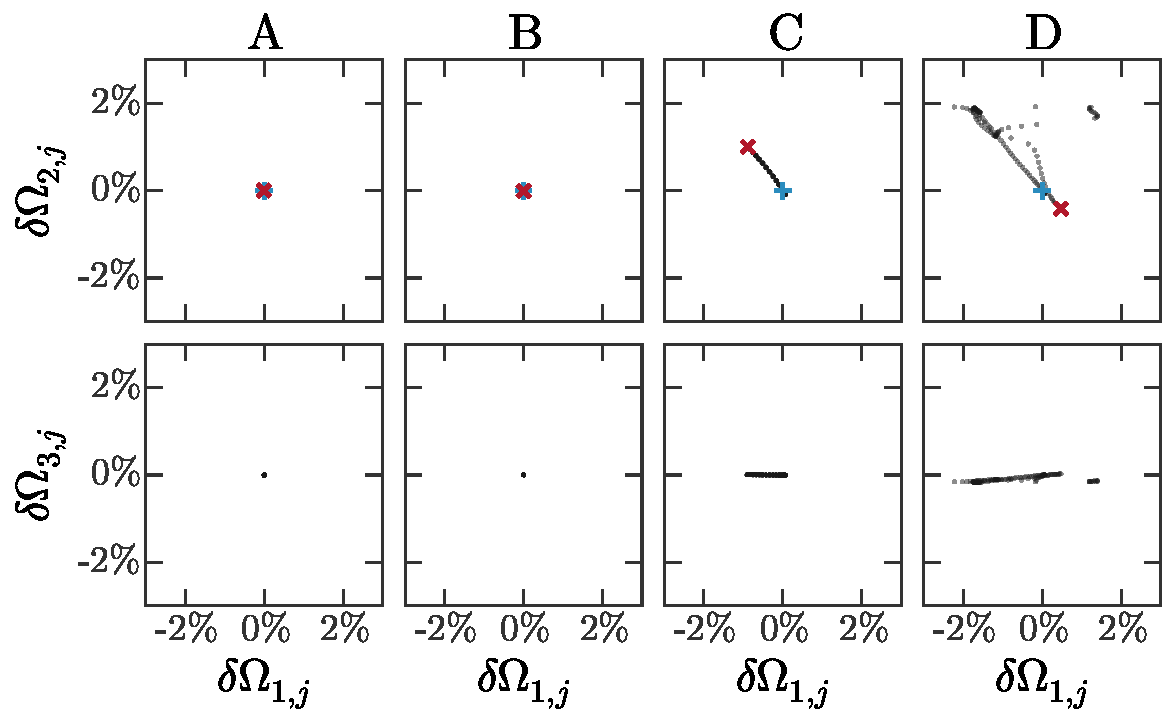
\includegraphics[width=\textwidth]{figures/ch3/freq-evolution.pdf}
\caption{Evolution of the fundamental frequencies computed over a total of 256
orbital periods for the four orbits, A, B, C, D. Plotted are the per cent
deviations of the frequencies computed in window relative to the value in the
initial window---that is, if $j$ is the index of a given time window, $\delta
\Omega_{1,j} = (\Omega_{1,j} - \Omega_{1,0})/\Omega_{1,0}$. The initial value is
shown as a blue plus sign and the final value is shown as a red x. The
frequencies are computed with a window width of $\approx$128 orbital periods,
and the window is shifted by one orbital period between each computation (each
grey point represents the fundamental frequencies computed in a single window).
For the regular orbits (A,B), the fractional variation is around $10^{-6}$ and
thus all points overlap on this scale. The weakly chaotic orbit (C) displays
frequency variations comparable to the spread in frequencies in
globular-cluster-like tidal debris. The frequency variations of the strongly
chaotic orbit (D) have a larger characteristic spread.}
\label{fig:four-orbits-freqs}
\end{center}
\end{figure}

% Figure - Ensemble frequencies
\begin{figure}[hp]%[p]
\begin{center}
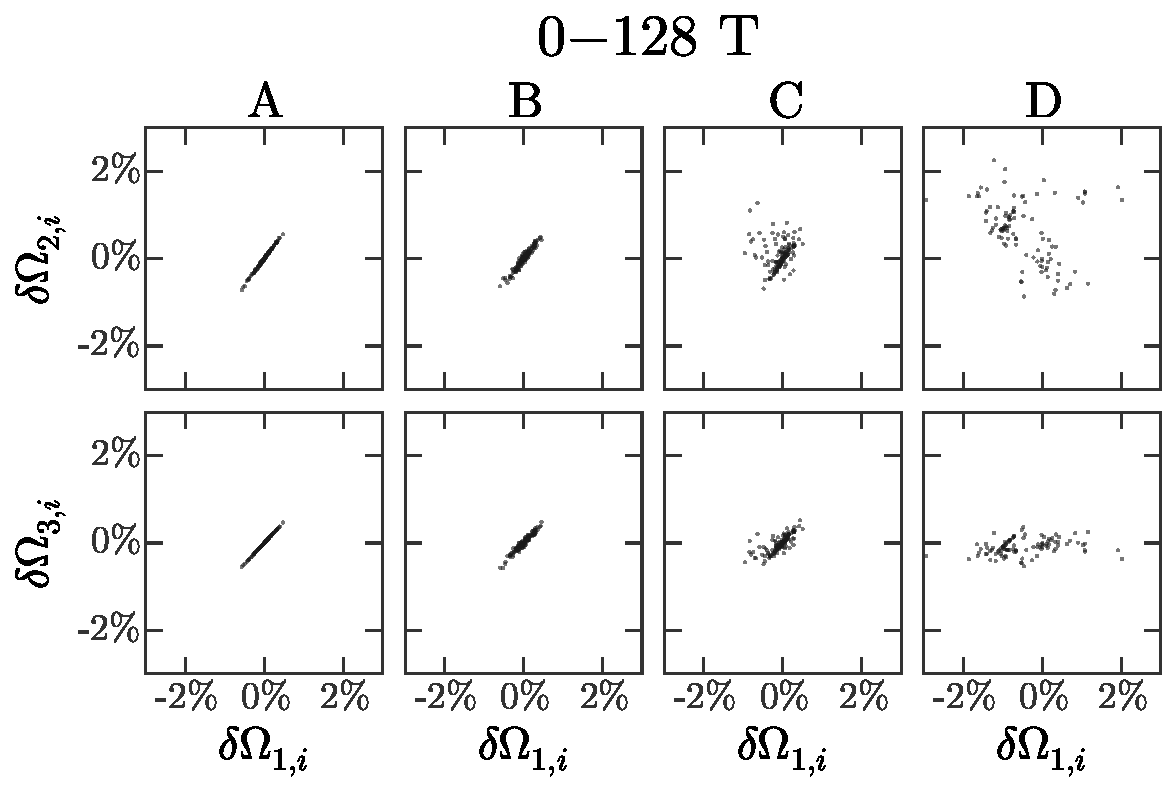
\includegraphics[width=\textwidth]{figures/ch3/ensemble-freqs-0.pdf}
\caption{Distributions of the fundamental frequencies for all orbits in
128-orbit ensembles generated around the four orbits, A, B, C, D. Plotted are
the per cent deviations of the frequencies of each ensemble orbit relative to
the frequencies of the parent orbit---that is, if $i$ is the index of a given
orbit and $i=0$ is the parent orbit, $\delta \Omega_{1,i} = (\Omega_{1,i} -
\Omega_{1,0})/\Omega_{1,0}$. All orbits are integrated for 128 orbital periods
to compute the frequencies. The near-resonant ensemble frequency distribution
(A) is nearly 1D, and thus the ensemble appears one-dimensional in
configuration-space (Figure~\ref{fig:ensembles}). The two largest eigenvalues of
the non-resonant ensemble frequency distribution (B) are closer, and thus the
ensemble spreads quicker, leading to a two-dimensional spread of debris in
configuration-space. Around both the weakly chaotic orbit (C) and strongly
chaotic orbit (D), chaotic diffusion increases the spread of the debris
significantly, leading to faster 3D spreading in configuration-space.}
\label{fig:ensemble-freqs0}
\end{center}
\end{figure}

% Figure - Ensemble frequencies
\begin{figure}[hp]%[p]
\begin{center}
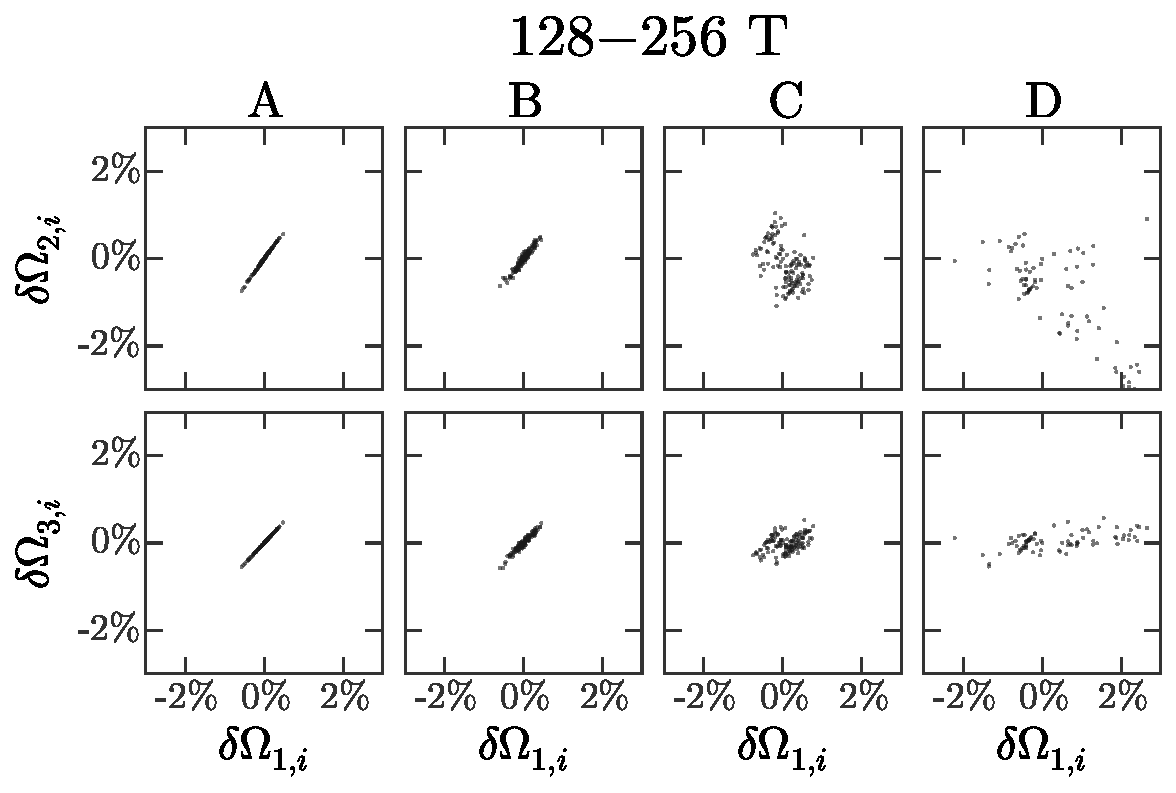
\includegraphics[width=\textwidth]{figures/ch3/ensemble-freqs-1.pdf}
\caption{Same as Figure~\ref{fig:ensemble-freqs0} but after integrating the same
orbits for another 128 orbital periods. The ensemble frequency distributions
around the regular orbits (A,B) appear nearly identical, whereas both the weakly
and strongly chaotic ensemble frequency distributions spread significantly.}
\label{fig:ensemble-freqs1}
\end{center}
\end{figure}

\section{Discussion: limitations and future work}\label{sec:ch4-discussion}

% Something about this: The timescales in this paper are not meant to be
% interpreted physically, as the potential is a very crude approximation to the
% total potential of a Milky-Way-like galaxy. The key point is that even when
% the mean chaos indicators predict a long chaotic timescale, streams may
% display enhanced density evolution over much shorter times. Tidal debris is
% sensitive to the small-scale, short-time evolution of orbital properties
% (e.g., the fundamental frequencies) induced by weak chaos.

We have shown that the Lyapunov and frequency diffusion times are indicators of chaos and that the frequency diffusion time resolves the detailed resonant structure of gravitational potentials, but the timescales predicted do not capture the importance of chaos for the density evolution of ensembles of orbits meant to mimic tidal debris. We have shown that small-scale but fast chaotic diffusion of frequencies can explain this enhanced mixing. In the sub-sections below, we discuss a few important limitations that remain for exploration in future work.

\subsection{The progenitor mass scale}

We have only considered low-mass progenitor systems such as globular clusters
because the intrinsic spreads in fundamental frequencies are small (0.1--0.5\%).
Small changes to the frequencies of the orbits of tidal debris stripped from
these progenitors due to chaotic processes will therefore cause observable
changes to the real-space morphology of the debris. For more massive progenitor
systems, the typical size and velocity dispersion of the debris will be larger
and thus the debris morphology will be less sensitive to small changes in
orbital properties. The mass-scale of the debris that will display enhanced
density evolution depends on the magnitude of weak chaos, which depends on the
orbit structure of a given potential. In potentials with more significant chaos,
debris disrupted from more massive progenitor systems may also display
`stream-fanning.' However, since the scale of the debris is larger it is more
likely that some orbits will exist in chaotic regions.

\subsection{Potential choice}

The potential considered in this work is `unrealistic' for the total potential
of a Milky-Way-like galaxy in that it is static, smooth, and does not contain
baryonic components. Simulations of forming galactic disks in cosmological
dark-matter haloes have shown that baryonic feedback and relaxation can
significantly change the inner distribution of dark matter and either make the
potential more spherical or oblate \citep{dubinski94,kazantzidis04, bryan13,
butsky15}. However, the significance of baryonic relaxation or of
time-dependence, triaxiality, and substructure on shaping the matter
distribution within the Milky Way is largely unknown. Here we briefly summarize
future directions for potential models:
\begin{itemize}
    \item \emph{Baryonic components}: \cite[][D08]{debattista08} and
    \cite[][V10]{valluri10} studied the orbit evolution induced by growing a
    baryonic disk in dark-matter haloes with various shapes and orientations
    (e.g., prolate, triaxial). In general, the authors find that the growth of a
    disk slowly deforms the orbits of mass tracers (e.g., dark matter particles)
    and preferentially populates tube or other `round' orbits (i.e. even the
    chaotic and box orbits fill a fairly spherical or oblate volume).
    Consequently, the inner shape of the potential becomes more oblate or
    spherical. If the inner haloes of galaxies are indeed close to spherical or
    oblate, the majority of orbits will be regular and chaos will be less
    important, however this is far from conclusive. We have found from simple
    experiments in superposing potential components that transition regions
    between potential shapes can significantly enhance the amount of chaos.
    Though superposing potentials is not realistic, it at least suggests that a
    more careful exploration of potential configurations is required to
    understand how complex, radius-dependent potential forms affect the amount
    and significance of chaos in galactic haloes.

\item \emph{Time dependence}: Galaxies are certainly not static systems. To
first order, galaxies grow in mass---for example, the spherically averaged mass
profile of dark-matter haloes evolves fairly predictably in cosmological
simulations \citep{wechsler02, buist14} after some initial period of stochastic
mass growth. The Milky Way has probably had a fairly calm accretion history over
the last 6 Gyr and therefore the mass growth may be similar to that seen in
simulations. This steady growth most likely does not alter the global structure
or shape of the potential. However, we also know from simulations that figure
rotation, baryonic feedback, and the accretion and phase-mixing of subhaloes do
perturb the global state of simulated haloes. \cite{deibel11} showed that by
adopting pattern speeds comparable to those found in cosmological simulations,
figure rotation generally acts to destabilize orbits (rather than stabilize
chaotic orbits in the equivalent static potential) and the resulting orbit
structure is that most regular orbits are associated with resonances. The
presence of and response to the Large and Small Magellanic Clouds may also
introduce significant (time-dependent) perturbations to the global potential of
the Milky Way \citep[e.g.,][]{besla10, gomez15}. In future work we will explore
the effect of these time-dependent processes on the chaotic dispersal of tidal
streams using live potentials from cosmological $N$-body simulations.

\item \emph{Substructure}: Cosmological simulations predict that dark-matter
haloes are filled with substructure in the form of dark matter subhaloes. If
they exist, these subhaloes may account for up to $\approx$1-10\% of the mass of
the dark matter \citep[e.g.,][]{diemand07} and therefore may contribute
significantly to and orbit in the large-scale potential of any galaxy.
Gravitational scattering due to subhalo interactions has been studied, however
in the haloes of galaxies where dynamical times are long, the scattering
cross-section for \emph{strong} encounters is small. Instead, the collective
effect of the subhaloes may instead act as a noise term in the Hamiltonian of
any halo orbit. This subhalo-induced heating---which depends on the mass
spectrum and distribution of subhaloes---may also act to simply increase the
magnitude of chaos along orbits, and destabilize sufficiently non-resonant
orbits \citep[see, e.g.,][]{kandrup00, siegalgaskins08}.

\end{itemize}

\subsection{Stream modeling}

Tidal stream modeling is one of the most promising ways to constrain the 3D mass
distribution around the Milky Way at distances of 10s to 100s of kpc. Methods
that use tidal streams to infer properties of the Galactic potential typically
operate by constructing models of the debris distribution using either the
present-day phase-space density \citep[e.g.,][]{varghese11, kuepper12,
kuepper15, gibbons14}, time-of-disruption phase-space density \citep{apw13,
apw14}, or the density in angle-action coordinates \citep{sanders14, bovy14}.
All of these methods may fail or produce uninterpretable results if modeling
globular-cluster streams on mildly chaotic orbits. For each of these methods, it
is important to understand the failures and biases introduced by ignoring
chaotic orbit evolution.

\subsection{Ophiuchus stream}

The Ophiuchus stream \citep{bernard14, sesar15a} appears to be a thin, short
tidal stream (deprojected length $\approx$1.5--2 kpc) near the Galactic bulge
with no apparent progenitor. At Galactocentric $R \approx 1$ kpc, $z \approx 5$
kpc, the orbits of the stream stars likely pass through the MW disk, feel the
triaxiality of the Galactic bar \citep[e.g.,][]{wegg13, wegg15}, and have short
orbital periods (relative to streams in the halo). It is possible that the
observed debris is the last remnants of the recently disrupted progenitor system
\citep{sesar15a}, however if a significant number of stars were stripped on
previous pericentric passages, this older debris may be `fanned' and still near
the observed portion of the stream. The fanned debris would have significantly
lower surface brightness and thus would be more difficult to detect. The
detection of this low-surface-brightness component would open up the possibility
that enhanced density evolution due to chaos is a dynamically relevant process
for thin streams in real galaxies, though \cite{carlberg15} has shown that it is
also possible to get short, high density segments of streams from debris formed
on eccentric orbits.

\section{Summary and Conclusions}\label{sec:ch4-conclusions}

We have considered here a simple triaxial gravitational potential chosen to
mimic the median properties of dark-matter haloes formed in dark-matter-only
simulations (or the large-scale properties of haloes formed in simulations with
baryonic effects). We have numerically computed the magnitude of chaos for a
large grid of iso-energy orbits in this potential using two independent methods
that have been used extensively to classify and characterize chaotic orbits: 1)
the Lyapunov exponent and 2) the frequency diffusion rate. From each of these
indicators, we compute a timescale over which chaos is likely to be important
and find that the majority of orbits have chaotic timescales greater than 100s
of orbital periods, however with the frequency diffusion rate we are still able
to resolve weak chaos. We then study the density evolution of small ensembles of
orbits generated around each orbit in the grid used for the previous experiment
and find that along some orbits classified as weakly chaotic---with chaotic
timescales of 100s of orbital periods---the orbit ensembles display enhanced
density evolution and reach a lower overall density faster than orbit ensembles
around nearby regular orbits (which mix due to phase-mixing alone). We explain
this discrepancy between the predicted chaotic timescale and the observed
effects of chaos on tidal debris by considering the nature of chaotic diffusion:
the classical chaos indicators are most sensitive to the slow, Arnold diffusion
process that can cause large changes to orbital properties, but small-scale
frequency evolution occurs over much shorter times as chaotic orbits
stochastically diffuse across the stochastic layers that surround many
resonances. The fundamental frequencies of a weakly chaotic orbit therefore vary
over a small region (bounded by nearby stable resonances), and when this
amplitude is comparable to or larger than the typical spread in frequencies of
tidal debris from the progenitor, the phase-space density of the debris will
evolve faster to a state of lower density relative to nearby regular orbits.

Our main results and conclusions are summarized as follows:
\begin{enumerate}
    \item ``stream-fanning'' of tidal streams on weakly chaotic orbits \citep[as
    seen in simulations by][]{pearson15} occurs due to small-scale chaotic
    evolution of the fundamental frequencies of the debris star orbits;
    \item the Lyapunov time and frequency diffusion time are powerful indicators
    of chaos, but do not capture the importance of small-scale chaotic diffusion
    for the density evolution of small ensembles of orbits (tidal debris);
    \item tidal debris becomes diffuse and thus harder to observe on weakly
    chaotic orbits when the small-scale chaotic diffusion of the fundamental
    frequencies has a scale comparable to the internal spread in frequencies of
    the debris;
    \item the details of the enhanced mixing along weakly chaotic orbits depends
    on the resonant structure of the potential;
    \item the covariance of the fundamental frequencies of an orbit over a given
    time window may be a better predictor of the importance of small-scale
    chaotic frequency diffusion on the resulting morphology of tidal debris.
\end{enumerate}

Our results provide a clear explanation of how and why the morphology of tidal
streams alone can be used to constrain the potential of the host galaxy. The
longest thin streams are most valuable for this effort because they have clearly
evolved for a long time, but the debris remains compact. For shorter thin
streams it will be hard to decouple the unknown evolution time from enhanced
density evolution from chaos. The mere existence of thin tidal streams in the
halo of the Milky Way either (1) provides useful information about the potential
on these scales by, e.g., implying a large degree of regularity, or (2)
indicates that the thin, long streams (e.g., GD-1) are on regular orbits. These
are not mutually exclusive---in fact, if the streams are on regular orbits, this
would be a powerful way to check or rule out possible potential models by
requiring that the progenitor orbits remain regular.

\section*{Acknowledgments}
The authors wish to thank Robyn Sanderson, Dan D'Orazio, David Merritt, and the
\emph{Stream Team} for useful comments and discussion. \chchchanges{The authors
additionally thank the referee, Walter Dehnen, for insightful comments that
greatly improved this \article.}

APW is supported by a National Science Foundation Graduate Research Fellowship
under Grant No.\ DGE 11-44155. KVJ and APW were partially supported by the
National Science Foundation under Grant No. AST-1312196 and NASA grant
NNX15AK78G. MV is supported in part by the University of Michigan's Elizabeth
Crosby Fund and the Office of the VP for Research and NASA ATP grant NNX15AK79G.
AHWK would like to acknowledge support from NASA through Hubble Fellowship grant
HST-HF-51323.01-A awarded by the Space Telescope Science Institute, which is
operated by the Association of Universities for Research in Astronomy, Inc., for
NASA, under contract NAS 5-26555.

This research made use of \project{Astropy}, a community-developed core
\project{Python} package for Astronomy \citep{astropy13}. This work additionally
relied on Columbia University's \emph{Hotfoot} and \emph{Yeti} compute clusters,
and we acknowledge the Columbia HPC support staff for assistance. This work used
the Extreme Science and Engineering Discovery Environment (XSEDE), which is
supported by National Science Foundation grant number ACI-1053575 \citep{xsede}.

%\bibliographystyle{apj}
%\bibliography{refs}

% appendix
\setcounter{section}{0}%
\renewcommand\thesection{\thechapter.\Alph{section}}
\section{Lyapunov exponents} \label{sec:ch4-lyapapdx}

% Using the definition of $w$ from Equation~\ref{eq:coords}, we can write
% Hamilton's equations as \footnote{A sum is implied with any repeated indices.}
% \begin{equation}
% 	\dot{w}_i = \mathcal{J}_{ik}\,\frac{\partial H}{\partial w_k} \label{eq:ham}
% \end{equation}
% where $\mathcal{J}_{ik}$ is the $2N \times 2N$ canonical Poisson tensor (also
% called the symplectic matrix) defined by
% \begin{equation}
%     \mathcal{J}_{ik} = \left( \begin{array}{c:c} 0 & \ident \\ \hdashline -\ident & 0 \end{array} \right)
% \end{equation}
% with $N$-dimensional identity matrices $\ident$. We will consider a nearby
% phase-space position, $w_i'$, separated from $w_i$ by an infinitesimal
% deviation, $\delta w_i$, such that $w_i' = w_i + \delta w_i$. We can expand to
% linear order in the deviation about the parent orbit and write the equations of
% motion for the deviation as
% \begin{align}
% 	\dot{\delta w_i} &= \mathcal{J}_{ik} \, \frac{\partial^2 H}{\partial w_k \partial w_m} \, \delta w_m =  \mathcal{J}_{ik}\, D_{km} \, \delta w_m \\
%     &= A_{im} \, \delta w_m
% \end{align}
% where $D_{km}$ is the Hessian matrix evaluated at the parent orbit. The general
% solution for this equation is
% \begin{equation}
% 	\delta w_i(t) = B_{im}(t) \, \delta w_i(0)
% \end{equation}
% where $\delta w_i(0)$ are the initial conditions for the deviation vector and
% $B_{im}$ is the solution matrix. For chaotic orbits, the maximum eigenvalue of
% the solution matrix to Eq.~\ref{eq:deviate} is positive real, leading to
% exponential divergence of nearby orbits.

If one is only interested in characterizing the degree of chaos, computing the full Lyapunov spectrum for an orbit is often not necessary. It is usually sufficient to compute an estimate of the maximum Lyapunov exponent by estimating the finite-time maximum Lyapunov exponent (FTMLE). Using the definition of $\boldsymbol{w}$ from Equation~\ref{eq:coords}, consider an orbit that is a small deviation away from the parent orbit, $\boldsymbol{w}' = \boldsymbol{w} + \delta\boldsymbol{w}$. If the parent orbit is chaotic, the norm of the infinitesimal deviation should grow exponentially with time with some characteristic rate, $\lambda$,
\begin{equation}
	\|\delta\boldsymbol{w}(t)\| = e^{\lambda \, t} \, \|\delta\boldsymbol{w}_0\|
\end{equation}
\citep[see, e.g.,][]{lichtenberg83,tabor89}. From this expression, we see that
\begin{equation}
	\lambda(t) = \frac{1}{t}\ln \frac{\|\delta \bs{w}(t)\|}{\|\delta \bs{w}_0\|} \label{eq:mle}
\end{equation}
where the maximum Lyapunov exponent is the limit as $t\rightarrow \infty$,
\begin{equation}
	\lambda_{\rm max} = \lim_{t\rightarrow\infty}\lambda(t). \label{eq:lmax}
\end{equation}
Numerically computing this quantity is not trivial because (1) obviously the limit to infinity is not possible and (2) the norm of the deviation vector $\|\delta \bs{w}(t)\|$ is expected to increase exponentially for chaotic orbits, leading to nonlinear evolution of the deviation and numerical problems. To circumvent these issues, it is sufficient to instead start a nearby orbit with some small initial deviation with norm $\delta_0$, integrate for a sufficiently small amount of time, $\tau$, then renormalize the deviation back to the initial norm \citep{benettin76}. There is no general way to determine $\tau$ except to perform convergence tests.
%The following pseudocode outlines this procedure:\footnote{see Gary for Python implementation?}\\
%\begin{algorithmic}[1]
%\State {\bf define} orbital integration timestep, $h$, and number of steps, $K$
%\State {\bf define} initial norm of deviation vector, $\delta_0$, to be sufficiently small
%\State {\bf define} renormalization integration period, $\tau \ll hK$
%\For{each timestep when integrating the main orbit, $\bs{w}(t)$}
%\State step forward the orbit and deviation vector orbit by one timestep, $t_{i-1} \rightarrow t_i$
%\If {a normalization timestep}
%\State measure and store the length of the deviation vector, $\delta_i = \|\delta \bs{w}_i\|$
%\State renormalize the length of the deviation vector, $\delta \bs{w}_i = \delta \bs{w}_i (\delta_0/\delta_i)$
%\EndIf
%\EndFor
%\end{algorithmic}
The FTMLE after a given number of timesteps, $N$, is then estimated as
\begin{equation}
	\lambda_N = \frac{1}{t_N}\sum_i^N \ln \frac{\|\delta \bs{w}(t_i)\|}{\|\delta \bs{w}_0\|} \label{eq:ftmle}
\end{equation}
where the $t_i$ are the times at which the renormalization occurs and the MLE is
estimated after a very long time to approximate the limit of
Equation~\ref{eq:lmax}.

For most regular orbits, deviations will grow linearly or as a power-law of
time. As we have seen in Section~\ref{sec:ch4-nldreview}, if the orbit is regular,
there exists a local transformation to action-angle variables where the angle
variables increase linearly with time, $\theta_i \propto \Omega_i t$. We can
look at small variations around the angle-space orbit,
\begin{align}
	\frac{d (\delta \theta_i)}{dt} &= \frac{\partial \Omega_i}{\partial J_k} \delta J_k
\end{align}
These equations are easily integrated:
\begin{align}
	\delta \theta_i(t) &= \delta \theta_i(0) + \left(\frac{\partial \Omega_i}{\partial J_k} \delta J_k \right) t
\end{align}
It's clear then that the norm of the deviation vector grows linearly with time:
\begin{align}
	\|\delta \bs{w}(t)\| &= \left[\sum_i (\delta \theta_i(t))^2 + \sum_i (\delta J_i)^2\right]^{1/2}\\
	&= \left[\sum_i \left(\delta \theta_i(0) + \frac{\partial \Omega_i}{\partial J_k} \delta J_k t\right)^2 + \sum_i (\delta J_i)^2\right]^{1/2}\\
	&\propto t.
\end{align}
From Equations~\ref{eq:mle} and \ref{eq:lmax} it is evident that any deviation vector that grows as a power law with time, $t^k$, will asymptote to 0 from the limit
\begin{equation}
	\lambda_{\rm max} \propto \lim_{t\rightarrow \infty} k \frac{\ln t}{t} = 0.
\end{equation}
At long times, the numerically computed MLE for a regular orbit should approach
0 as $t^{-1}$. For chaotic orbits, the divergence is exponential, and the limit
should converge to the rate of the exponential: the Lyapunov exponent. In
practice, the MLE is often estimated as the mean of $\lambda_N$ after the
summation diverges from power-law behavior. For weakly chaotic orbits, reliable
computation of the MLE may take integration of thousands of orbital periods.

\section{SuperFreq}\label{sec:ch4-naffapdx}

\renewcommand{\thefigure}{\thesection.\arabic{figure}}

The NAFF algorithm operates on numerically integrated orbital time-series (i.e.
positions and velocities at a set of equally spaced times). Complex combinations
of the phase-space coordinates of the orbit are Fourier-transformed using a
standard FFT and the resultant spectrum is then searched for the strongest
frequency component; this serves as an initial guess for the frequency of a
particular Fourier component. Solving for the frequency that maximizes the
Fourier integral of the FFT with a particular window function allows for a more
accurate determination of the frequency. It has been shown that this accuracy
converges much faster than the typical $\inttime^{-1}$ expected for a standard
FFT by using a window function of the form
\begin{equation}
	W(\tau=t/\inttime) = \frac{2^p \, (p!)^2}{(2p)!} \left( 1 + \cos \pi \tau\right)^p
\end{equation}
where $\inttime$ is the integration time \citep{laskar99}. Once the strongest
frequency component is found, it is subtracted from the spectrum and the process
is repeated iteratively. This procedure generates a table of frequencies for
each component of motion which must then be searched for the three fundamental
frequencies. The original implementations of NAFF have used $p=1$
\citep[e.g.,][]{laskar93, valluri98}, but we have chosen to use $p=4$. With a
higher order window function, the central peak is broadened, but the amplitudes
of the side lobes decrease faster \citep[see][]{hunter02}; we have found that
this additional damping of the side lobes allows for more reliable determination
of frequencies from strongly chaotic orbits.

\setcounter{figure}{0}
\begin{figure}
\begin{center}
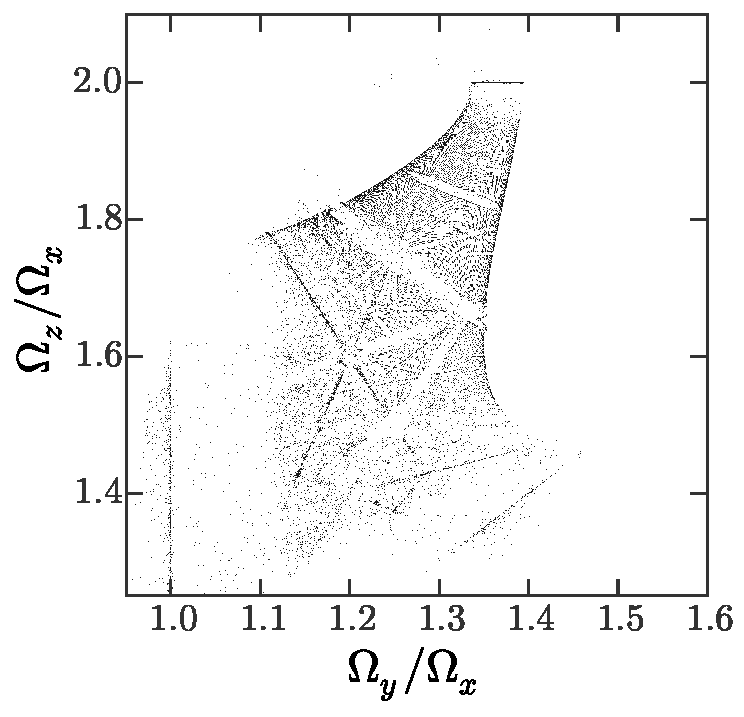
\includegraphics[width=\textwidth]{figures/ch3/log-freqmap.pdf}
\caption{ A reproduction of Figure~3.45 from \citep{binneytremaine} as a
validation of our frequency analysis code: Frequency ratios for 100000 isoenergy
orbits integrated in a triaxial logarithmic potential. Linear features are
resonances---stable resonances appear as dark lines, unstable resonances appear
as linear gaps.} \label{fig:logfreqs}
\end{center}
\end{figure}

\superfreq\ recovers the fundamental frequencies for an orbit faster (with a
fewer number of terms) when the coordinates used are `close' to the angle
variables \cite[PL96;][]{papaphilippou96}. PL96 show that a good choice of
coordinates for tube orbits are the Poincar\'e symplectic polar coordinates, a
set of canonical coordinates similar to cylindrical coordinates. When computing
the frequencies for tube orbits, we first align the circulation about the
$z$-axis through rotation, transform to Poincar\'e polar coordinates, then use
\superfreq\ to measure the fundamental frequencies. We could equivalently use
the Cartesian time series, but the convergence of terms is slower (the
amplitudes of successive terms decrease slower for Cartesian coordinates). We
have tested that our implementation of \superfreq\ returns the same fundamental
frequencies in either case for a set of tube orbits. For box orbits, the motion
is close to separable in each Cartesian component and we therefore use Cartesian
coordinates for estimating the frequencies for these orbits.

Figure~\ref{fig:logfreqs} shows a validation of our frequency analysis code in
which we reproduce the frequency map at a fixed energy of an axisymmetric,
logarithmic potential \cite[][pg. 260, Figure~3.45]{binneytremaine}. Plotted are
the (Cartesian) frequency ratios recovered for a grid of iso-energy, box orbits
integrated in the potential
\begin{equation}
	\Phi(x,y,z) = \frac{1}{2}\ln\left(x^2 + (y/0.9)^2 + (z/0.7)^2 + 0.1\right). \label{eq:logpotential}
\end{equation}
Following \cite{binneytremaine}, we generate a grid of orbits on the
equipotential surface $\Phi(x,y,z) = 0.5$ (we use a grid with 100000 orbits
compared to their 10000 orbits). Each orbit is integrated for $\approx$40
orbital periods. In this figure, stable resonances appear as linear
over-densities and unstable resonances appear as linear under-densities or gaps.
The regularity of the points in this map reflects the input grid of initial
conditions. Points that appear to be erratically scattered are chaotic orbits
where the frequencies change with time.

% ----------------------------------------------------------------------------------

\renewcommand{\thefigure}{\arabic{figure}}

% Figure ??
%\begin{figure}[!p]
%\begin{center}
%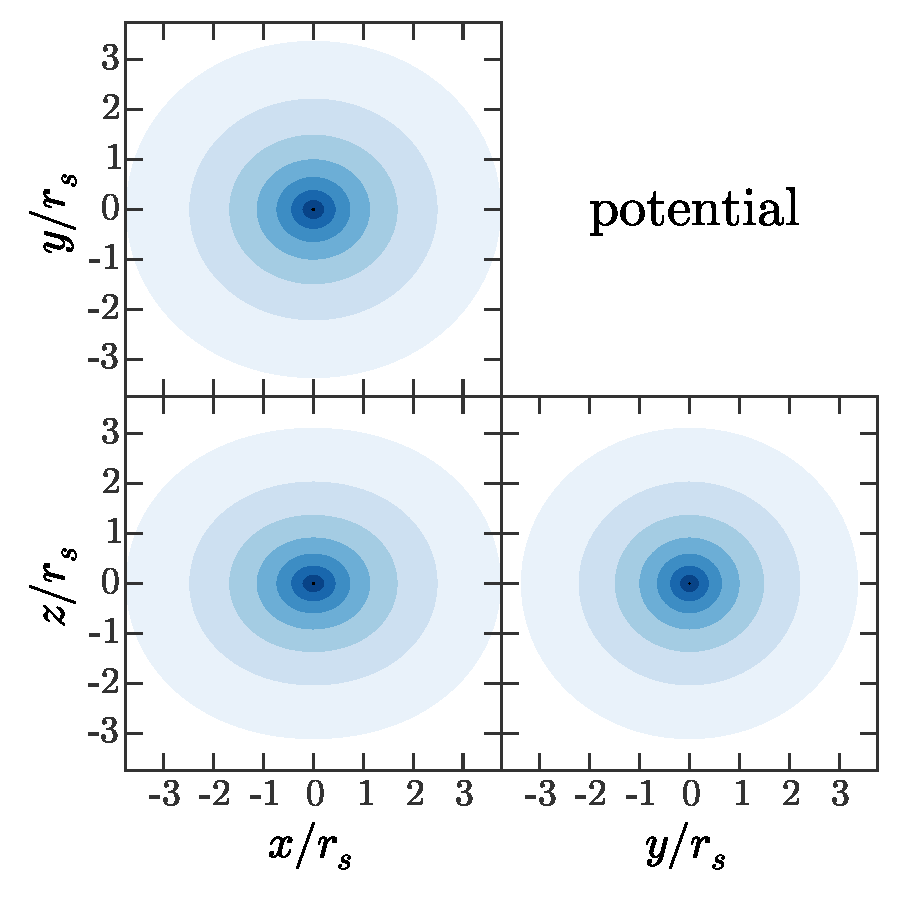
\includegraphics[width=\textwidth]{figures/ch3/potential.pdf}
%\caption{Equipotential contours for the triaxial NFW potential considered in this work. There are eight contour levels evenly spaced and linear in the value of the potential. } \label{fig:potential}
%\end{center}
%\end{figure}

\renewcommand\thesection{\thechapter.\arabic{section}}

	\chapter[Chaotic fanning of the Ophiuchus stream]{Chaotic fanning of the Ophiuchus stream}
\label{ch:chaos-ophiuchus}
% \let\thefootnote\relax\footnotetext{This section contains text from an article published in XXX. Portions of this paper's introduction now appear in the introduction to this dissertation.}

% TODO: do I need \usepackage[caption=false]{subfig}?
% \usepackage{multirow}

% TODO this could change after referee response...

\newcommand{\lyapexp}{\lambda_{\rm max}}
\newcommand{\lyapt}{t_\lambda}

%\title{Spending too much time at the Galactic bar: chaotic fanning of the Ophiuchus stream}
%\author{Adrian M. Price-Whelan\altaffilmark{\colum,\adrn},
%            Branimir Sesar\altaffilmark{\mpia},
%            Kathryn V. Johnston\altaffilmark{\colum},
%            Hans-Walter Rix\altaffilmark{\mpia}
%}
%
%% Affiliations
%\newcommand{\colum}{1}
%\newcommand{\adrn}{2}
%\newcommand{\mpia}{3}
%
%\altaffiltext{\colum}{Department of Astronomy,
%                      Columbia University,
%                      550 W 120th St.,
%                      New York, NY 10027, USA}
%\altaffiltext{\adrn}{To whom correspondence should be addressed: adrn@astro.columbia.edu}
%\altaffiltext{\mpia}{Max-Planck-Institut f\"ur Astronomie,
%                     K\"onigstuhl 17, D-69117 Heidelberg, Germany}
%
%\begin{abstract}
%The Ophiuchus stellar stream is peculiar: (1) its length is short given the age of its constituent stars, and (2) several probable member stars that lie close in both sky position and velocity have dispersions in these dimensions that far exceed those seen within the stream.
%The stream's proximity to the Galactic center suggests that the bar must have a significant influence on its dynamical history: The triaxiality and time-dependence of the bar may generate chaotic orbits in the vicinity of the stream that can greatly affect its morphology.
%We explore this hypothesis with models of stream formation along orbits consistent with Ophiuchus' properties in a Milky Way potential model that includes a rotating bar.
%We find that in all choices for the rotation parameters of the bar, orbits fit to the stream are strongly chaotic.
%Mock streams generated along these orbits qualitatively match the observed properties of the stream: because of chaos, stars stripped early generally form low-density, high-dispersion ``fans'' leaving only the most recently disrupted material detectable as a strong over-density.
%Our models predict that there should be more low-surface-brightness tidal debris than detected so far, likely with a complex phase-space morphology.
%The existence of or lack of these features around the Ophiuchus stream would provide an interesting constraint on the properties of the Milky Way bar and would help distinguish between formation scenarios for the stream.
%This is the first time that chaos has been used to explain the properties of a stellar stream and is the first demonstration of the dynamical importance of chaos in the Galactic halo.
%The existence of long, thin streams around the Milky Way---presumably formed along non- or weakly-chaotic orbits---may represent only a subset of the total population of disrupted satellites.
%\end{abstract}
%
%\keywords{
%  Galaxy: halo
%  ---
%  globular clusters: general
%  ---
%  stars: kinematics and dynamics
%  ---
%  Galaxy: structure
%  ---
%  Galaxy: kinematics and dynamics
%}

\section{Introduction}\label{sec:introduction}

The Ophiuchus stream \citep{bernard14, sesar15a} is a recently discovered
stellar tidal stream that sits above the Galactic bulge at a Galactocentric
radius and height $(R,z) \approx (1.5, 4.3)~{\rm kpc}$. All observational
evidence suggests that the stream is a completely disrupted globular cluster:
The stream stars have (1) a small positional dispersion orthogonal to the
extended direction of the stream (width $\approx$10 pc, length $\approx$1.5
kpc); (2) no detectable over-density along the stream that could be the
progenitor system; (3) a small velocity dispersion $\approx$0.4 ${\rm km}~{\rm
s}^{-1}$; and (4) an old stellar population ($\approx$12 Gyr) estimated from
isochrone fitting \citep[][hereafter S15]{sesar15a}.

There are a number of peculiarities about the observed kinematics of the
Ophiuchus stream. For example, the de-projected length of the visible part of
the stream is short given the age of its stellar population ($\approx$1.5 kpc).
S15 fit an orbit to the kinematics of the stream stars in a static, axisymmetric
model for the gravitational field of the inner Galaxy and ran N-body simulations
of globular clusters on this orbit. S15 find that---on this orbit---the portion
of the stream visible as an over-density in main-sequence stars must have been
formed in the last $\lesssim$400 Myr for the stream to remain as short as it is
observed. This dynamical age is at odds with the old ($\approx$10--12 Gyr)
stellar population: The abrupt end of the stream suggests that the cluster
apparently fully disrupted at once in the last 400 Myrs. Another puzzle is the
existence of blue horizontal branch (BHB) stars close to the stream (within a
few degrees) with similar radial velocities, but with a large dispersion in both
sky position and velocity \citep[][hereafter S16]{sesar16}. The stream has a
very distinct and large line-of-sight velocity ($\approx$290 \kms) and is
therefore easily detected above the background halo population. Four BHB stars
have been detected with line-of-sight velocities $>230~\kms$ that lie close to
an extrapolation of the stream on the sky. This makes them likely members of the
stream, as their velocities are in stark contrast to the background halo
population (see Section 4, S16). Yet, they have a velocity dispersion
$\approx$75 times larger than the measured internal velocity dispersion of the
stream stars. These stars hint at the existence of associated low-density,
high-dispersion features that were not modeled in S15 and are not predicted by
the $N$-body simulations from this prior work, which assume a sudden, total
disruption of the stream progenitor.

% ---------------------------------------------------------------------------------
\begin{figure*}[!tbp]
\begin{center}
%\includegraphics[width=0.7\textwidth]{figures/potentials-four}
\includegraphics[width=\textwidth]{figures/ch4/potentials-four}
\caption{{\it Left column:} Circular velocity curves along the Sun-Galactic
center line for a representative barred MW potential model (top left) and for
the static MW potential model (bottom left). Solid black line shows total (sum
of all components), lines below show a decomposition by potential components.
Vertical grey bar shows approximate position of the Sun, horizontal grey bar
shows roughly the range in measured circular velocity of the Sun. {\it Right
column:} Contours of constant surface density for a barred MW potential (top
right) and the static MW potential model (bottom right). Four contours are drawn
per decade in surface density between $10^7$ and $10^{12}~\msun~{\rm kpc}^{-3}$.
Note the perturbation from the bar potential within Galactocentric radius $r
\lesssim 4~{\rm kpc}$. The Sun's position is indicated by the `$\odot$' symbol.
}
\label{fig:potentials}
\end{center}
\end{figure*}

The orbit fit and $N$-body simulations in S15 used a static, axisymmetric
potential to represent the Milky Way potential, but it is well-known that the
Galactic bulge contains a triaxial, rotating, bar-like structure several kpc in
size \citep[e.g.,][]{blitz91, weinberg92, dwek95, wegg13}. Given the proximity
of the stream to the center of the Galaxy, the time-dependent, triaxial
potential of the Galactic bar must be taken into account when modeling the orbit
of the Ophiuchus stream. The presence of a bar-like perturbation to the
potential will change the orbit of the stream progenitor and the orbit structure
in the inner galaxy \citep{zotos12, portail15b, gajda15}. Bar-like features can
also introduce a significant number of chaotic orbits in their vicinity
\citep{weinberg15} and generate resonances that may also affect stream formation
\citep{hattori15}.

Recent work has shown that dynamical chaos can dramatically alter the density
evolution of tidal streams \citep[e.g.,][]{fardal14, apw15-chaos}. Along certain
chaotic orbits, the stream stars will spread much faster in 3D position than
from ordinary phase-mixing and, depending on the orbital phase at which the
stream is observed, may develop large, low-density ``fans'' of stars at the ends
of a stream \citep{pearson15, apw15-chaos}. As a first application of this
theoretical understanding, we study whether stream-fanning---chaotic or simply
from density evolution in a triaxial, time-dependent potential---could plausibly
explain the observed properties of the Ophiuchus stream. In particular, we
consider whether such models can reproduce:
\begin{enumerate}
	\item the apparent shortness and fast density truncation of the stream;
	\item the increased positional dispersion of the four new candidate members from S16;
	\item the large velocity dispersion of the S16 stars.
\end{enumerate}
We do not aim to perfectly represent the observed data, but rather to explore
the plausibility of explaining the peculiarities of the stream using chaotic
stream fanning. Note that an alternate model was recently proposed that instead
places the stream progenitor on an orbit in resonance with the bar
\citep{hattori15}. We discuss the differences between these two models in
Section~\ref{sec:discussion}.

In Section~\ref{sec:method} we describe the methods used in this work: in
Section~\ref{sec:potential} we describe the models we use for the gravitational
potential of the Galaxy, in Section~\ref{sec:orbitfit-nonapdx} we outline the
probabilistic procedure we use to fit orbits to the stream data (explained in
detail in Appendix~\ref{sec:orbitfit}), and in Section~\ref{sec:mocks} we
explain the simple method we use to generate mock streams. In
Section~\ref{sec:results1} we discuss the results from fitting orbits to the
data in a static, axisymmetric potential model and several potential models with
a time-dependent bar. In Section~\ref{sec:results2} we generate mock streams
along these orbits to argue that chaotic stream-fanning is a plausible
explanation for the observational peculiarities of the Ophiuchus stream. We
discuss the implications of this work and possibilities for future work in
Section~\ref{sec:discussion} and we conclude in Section~\ref{sec:conclusions}.

\section{Methods}\label{sec:method}

Our goal is to (1) assess whether the Galactic bar can produce chaotic orbits in
the vicinity of the Ophiuchus stream and (2) determine if chaotic density
evolution of tidal debris stripped from the progenitor of this stream can
explain the apparent shortness of the stream and low-density, high-dispersion
stars beyond the extent of main sequence stars observed in PS1. In this section,
we describe the potential models we use to represent the galaxy and outline the
methods we use to detect and quantify the strength of chaos for individual
orbits. We then describe the likelihood function we use for fitting orbits to
the stream stars. Finally, we describe how we generate mock stellar streams for
a progenitor on a given orbit.

Throughout we assume the Sun is at Galactocentric position $(x,y,z) =
(-8.3,0,0)~{\rm kpc}$ \citep[e.g.,][]{schoenrich12} with velocity $(v_x,v_y,v_z)
= (-11.1, 250, 7.25)~\kms$ \citep[e.g.,][]{schoenrich10, schoenrich12}.

\subsection{Potential models}\label{sec:potential}
To integrate orbits and to compute chaos indicators we must choose a
gravitational potential model to represent the potential of the Milky Way. The
key feature of the potential that we would like to capture is the
time-dependence and triaxiality of the Galactic bar. Recent work has used
stellar number counts of Red Clump giant stars in the Galactic bulge to
constrain dynamical models of the bar \citep{portail15}. Measurements of the
total mass of the bar feature from this study are largely consistent with past
work \citep[e.g.,][]{wang12}, however the measured pattern speed and present bar
angle are significantly discrepant and this difference is not fully understood.
We construct a parametrized potential model consisting of a triaxial,
time-dependent (rotating) bulge component added to simple models for the disk
and halo of the Milky Way. We describe below how we fix the parameters of the
disk, halo, and bar or bulge component, but explore different choices for the
time-dependence and orientation of the bar. We also define a static potential
with a spherical bulge for comparison.

These potential models are meant to be representative rather than definitive.
The uncertainty in the Milky Way potential within Galactocentric radii of
$r\lesssim 4~{\rm kpc}$ and outside of $r\gtrsim 15~{\rm kpc}$ are large enough
that trying to match the exact density distribution of the Ophiuchus stream is
not a useful exercise. Instead, we consider qualitatively different potentials
that allow us to isolate and study the affect of chaotic stream-fanning of tidal
debris in the vicinity of the stream.

\subsubsection{Barred potential}
We use a spherical Navarro-Frenk-White potential to represent the dark matter
halo \citep{navarro96} parametrized as
\begin{align}
	\Phi(r) &= -v_h^2\,\frac{\ln{(1 + r/r_s)}}{r/r_s}\label{eq:nfw}
\end{align}
and a Miyamoto-Nagai potential for the disk \citep{miyamoto75}. For the bar
component, we use a basis function expansion (BFE) of the potential and density
of the bar with expansion coefficients derived for a triaxial, exponential bar
density \citep[][hereafter W12]{wang12}. We use the pre-computed expansion
coefficients used in W12, which were computed from a low-order expansion of the
triaxial bar density used in \citet{dwek95}.\footnote{The coefficients presented
in W12 are for just the cosine terms (the $A_{lm}$ in \citet{hernquist92} or the
$S_{nlm}$ in \citet{lowing11}) because all sine terms have zero coefficients for
a triaxial density function.} We have implemented the BFE computation of the
potential, density, and gradient of the potential in \texttt{C} and \python\ and
the code is publicly available on
\github.\footnote{\url{https://github.com/adrn/biff}}

The BFE representation fixes the axis ratios of the bar---that is, the
exponential scale lengths along the three axes of the bar were adopted from
\cite{dwek95} when the expansion coefficients were calculated in W12; all other
potential parameter values are given in Table~\ref{tbl:potential-params-barred}.
The mass of the halo is fixed and the mass of the disk and bar are varied in
order to qualitatively reproduce the flatness and amplitude of the circular
velocity curve of the Milky Way \citep{bovy12}. Figure~\ref{fig:potentials}, top
left shows the circular velocity along the line connecting the Sun to the
Galactic center in this model (the Galactic $x$ axis).
Figure~\ref{fig:potentials}, top right shows contours of constant surface
density for a face-on (left) and edge-on (right) view of this potential model
with the bar angle set to $20^\circ$ \citep[compare to, e.g., Figure 3
in][]{portail15}. We consider a grid of nine parameter combinations of bar angle
and pattern speed. Model names and parameter values are given in
Table~\ref{tbl:bar-specific}.

\begin{table}[ht]
\begin{center}
	\begin{tabular}{ c | c | c }
	         \toprule
	         Component & Parameter & Value \\\toprule
		Disk & $M_{\rm disk}$ & $4 \times 10^{10}~\msun$ \\
		& $a$ & 3~{\rm kpc}\\
		& $b$ & 0.28~{\rm kpc} \\\midrule
		Spheroid & $M_{\rm sph}$ & $5 \times 10^{9}~\msun$ \\
		& $c$ & 0.2 \\\midrule
	         Halo & $v_c$ & 185.8~\kms\\
		& $r_s$ & 30~kpc \\
		Bar & $M_{\rm bar}$ & $1.8 \times 10^{10}~\msun$ \\
		\bottomrule
		\end{tabular}
	\caption{The disk potential scale lengths ($a$, $b$) were adopted following
	\citep{bovy15-galpy} to match the exponential scale length of the disk
	\citep{bovyrix13} and local dark-matter density
	\citep[e.g.,][]{bovytremaine12}. The halo mass scale is set by specifying
	the circular velocity at the scale radius, $v_c$, and the scale velocity in
	Equation~\ref{eq:nfw} is given by $v_h^2 = v_c^2 / (\ln2 - 1/2)$. The bar
	mass is taken from recent 3D density modeling of red clump stars in the
	Galactic bulge \citep{portail15}. The other bar parameters are listed in
	Table~\ref{tbl:bar-specific} next to the corresponding model name.
	\label{tbl:potential-params-barred}}
\end{center}
\end{table}

\begin{table}[ht]
\begin{center}
	\begin{tabular}{ c | c | c }
	         \toprule
	         Name & $\alpha$ [deg] & $\Omega_p$ [${\rm km}~{\rm s}^{-1}~{\rm kpc}^{-1}$] \\\toprule
		bar1 & 20 & 40\\
		bar2 & 20 & 50\\
		bar3 & 20 & 60\\
		bar4 & 25 & 40\\
		bar5 & 25 & 50\\
		bar6 & 25 & 60\\
		bar7 & 30 & 40\\
		bar8 & 30 & 50\\
		bar9 & 30 & 60\\
		\bottomrule
		\end{tabular}
	\caption{Present-day bar angle ($\alpha$) and pattern speed ($\Omega_p$) for
	the nine parameter pairs considered in this work. These values span the
	range of recent measurements from a variety of techniques \citep{dwek95,
	wang12,wang13,wegg13}. \label{tbl:bar-specific}}
\end{center}
\end{table}

\subsubsection{Static potential}

For comparison, we also define a time-independent potential model with a purely
spherical bulge. In this model, we set the bar mass to 0 and instead add a
spheroidal component represented with a Hernquist potential \citep{hernquist90}.
Parameters for this potential model are given in
Table~\ref{tbl:potential-params-static}. Figure~\ref{fig:potentials}, bottom
left shows the circular velocity along the line connecting the Sun to the
Galactic center in this model (the Galactic $x$ axis).
Figure~\ref{fig:potentials}, bottom right shows contours of constant surface
density for a face-on (left) and edge-on (right) view of this potential model.

\begin{table}[ht]
\begin{center}
	\begin{tabular}{ c | c | c }
	         \toprule
	         Component & Parameter & Value \\\toprule
		Disk & $M_{\rm disk}$ & $6 \times 10^{10}~\msun$ \\
		& $a$ & 3~{\rm kpc}\\
		& $b$ & 0.28~{\rm kpc} \\\midrule
	         Halo & $v_c$ & 185.8~\kms\\
		& $r_s$ & 30~kpc \\\midrule
		Spheroid & $M_{\rm sph}$ & $1.2 \times 10^{10}~\msun$ \\
		& $c$ & 0.3 \\
		\bottomrule
		\end{tabular}
	\caption{Same as Table~\ref{tbl:potential-params-barred}, except: the disk mass is increased to account for removing the bar component, a spheroidal bulge component is added. \label{tbl:potential-params-static}}
\end{center}
\end{table}

\subsection{Fitting orbits to the Ophiuchus stream}\label{sec:orbitfit-nonapdx}

In each of the potentials described above, we fit orbits to the measured
kinematics of BHB stars that are high-likelihood members of the Ophiuchus stream
\citep{sesar15a, sesar16}. The details of this procedure and a definition of the
likelihood function we use are presented in Appendix~\ref{sec:orbitfit}. We use
an ensemble Markov Chain Monte Carlo (MCMC) algorithm \citep{goodman10}
implemented in \python\ (\package{emcee}) to generate samples from the posterior
distribution over the parameters in our orbit-fitting model
\citep{foremanmackey13}. The algorithm uses an ensemble of individual
``walkers'' to adapt to the geometry of the parameter-space being explored. In
all cases, we use 80 walkers (8 times the number of parameters).

To initialize these walkers, we first run an optimization routine to maximize
the likelihood: We use the Powell algorithm implemented in \package{Scipy}
\citep{powell64, scipy} to minimize the negative, log-likelihood. To generate
initial conditions for the walkers, we sample from Gaussian distributions
centered on the maximum likelihood values. For the coordinates, we set the
dispersions of these Gaussians to 1/1000 of the median uncertainties of the
stars. For the nuisance parameters, we set the dispersions to 1/1000 of their
maximum likelihood values.

For each potential, we run the MCMC walkers for a burn-in period of 512 steps
and then re-initialize the walkers from their positions at the end of this run.
This erases any relics of the initialization procedure outlined above. After
burn-in, we run the walkers for an additional 512 steps. For each parameter, we
compute the autocorrelation times, $\tau$, of the Markov chains and thin the
chains by taking every $2\tau$ sample. This reduces the number of samples, but
ensures that our posterior samples are effectively independent.

\subsection{Generating mock streams}\label{sec:mocks}

To generate mock stellar streams, we use the method presented in
\citet{fardal14}: Star particles are `released' from a progenitor system near
the Lagrange points with a dispersion in position and velocity that is set by
the mass and orbit of the progenitor. We draw samples from the posterior
probability distributions over orbital parameters from fitting orbits to the
stream star members and use these as the progenitor orbital parameters
(Section~\ref{sec:orbitfit}). For a given progenitor orbit---the 6D position of
the orbit today---we integrate the orbit backwards in time for a given
integration period. From the endpoint of the backwards-integration (e.g., the
past position), we begin integrating the orbit forward in time, but now at each
time-step a star particle is released near each of the Lagrange points of the
progenitor. The position of the Lagrange points and the scale of the dispersion
in position and velocity are set by the progenitor mass, $m$. The star particles
are drawn from Gaussians centered on the Lagrange points (in position) and the
progenitor (in velocity) and the full parametrization of the release
distribution is given in \cite{fardal14}. This method has been shown to
reproduce the morphologies of $N$-body simulations of stellar streams, but
requires far less computing time because it relies only on integrating
test-particle orbits.

% ---------------------------------------------------------------------------------
\begin{figure}[!tbp]
\begin{center}
%\includegraphics[width=0.5\textwidth]{figures/orbitfits}
\includegraphics[width=0.75\textwidth]{figures/ch4/orbitfits}
\caption{ Results from fitting orbits to BHB stars associated with the Ophiuchus
stream in the static and barred potential models. Data used for computing the
likelihood are shown as black points with grey error bars. The four ``fanned''
BHB stars from S16 excluded from the likelihood computation are shown as grey
squares. Error bars may sometimes be smaller than the point size. Lines (blue)
show sections of orbits integrated forward and backwards from initial conditions
drawn from the posterior samples generated by MCMC (See
Section~\ref{sec:orbitfit}). Note that the four higher dispersion stars (the
four stars with highest longitude) were not used when computing the likelihood
and are only shown for completeness. Though these four stars are significant
outliers relative to the extrapolated orbit, they are (1) at the correct
distance and sky position relative to the stream and (2) have velocities
$\approx$2.5$\sigma$ discrepant with the halo velocity distribution in this
region.}
\label{fig:orbitfits}
\end{center}
\end{figure}

We make one modification to this method based on the idea that the Ophiuchus
stream progenitor has been fully-disrupted. We add an additional parameter to
the stream generation routine to specify the time of disruption, $\tau_d$. At
this time, we set the offset of the Lagrange point to 0: In terms of the
parametrization in \citep{fardal14}, we set $k_r = 0$ and $k_{vt}=0$ but
preserve the dispersion in the release radius and velocity. Any star released
after $\tau_d$ is released with a small dispersion around the progenitor orbit
but no offset. This mass-loss history is intended to mimic the expected gradual
evaporation of a globular cluster over a tidally-limited boundary (i.e. driven
by two-body relaxation and gravitational shocks over many Gigayears) with final
disruption likely to occur once the tidal boundary is less than the core radius
of the cluster. The physics of this disruption is not followed exactly but
rather the disruption rate and final disruption time are set by the hypothesis
that the most recent combined pericenter and disk shock fully disrupted the
cluster, but, critically, that the cluster has been losing debris over its
entire orbital history.

\section{Results I: Orbit fits and chaos}\label{sec:results1}

Figure~\ref{fig:orbitfits} summarizes our results from fitting orbits to the BHB
stream stars. Shown in each panel are the high-probability Ophiuchus stream
stars (black points, to which orbits are fit) and orbits integrated from samples
from the posterior probability over orbital parameters (blue lines). The four
``fanned'' BHB stars from S16 are shown as grey squares and are not included in
the orbit fitting procedure. We only show one of the barred potentials: The
end-to-end integration time of the orbit over the observed extent of the stream
is only $\approx$6 Myr, so the derived orbits are extremely similar in all
potentials (the time-dependence of the bar potential is not significant over
such short timescales). The orbital periods are typically $\approx$170--200 Myr
with pericenters $r_p \approx 4~{\rm kpc}$ and apocenters $r_a \approx
12$--$15~{\rm kpc}$. Though the coordinate and velocity parameter values in
observed coordinates are very similar between each potential model, the
resulting orbits are quite different. For the posterior samples in each
potential, we take the mean values of the coordinate and velocity parameters and
convert to Galactocentric coordinates (e.g., Table~\ref{tbl:param-means}).
Figure~\ref{fig:orbits-yz} shows projections of these ``mean'' orbits in each
potential model.

For the posterior samples in each potential, we also compute the maximum
Lyapunov exponent (MLE, $\lyapexp$) and corresponding Lyapunov \emph{time}
($\lyapt = 1/\lyapexp$) to assess whether each orbit is chaotic. For strongly
chaotic orbits, the Lyapunov time is still an appropriate indicator of chaos and
of the timescale over which chaos is important for tidal debris
\citep{apw15-chaos}. Figure~\ref{fig:lyapunov-hist} shows distributions of
Lyapunov times for orbits drawn from the posterior distributions from orbit
fitting in each potential model. All orbits in the static potential have
Lyapunov times $\lyapt > 20~{\rm Gyr}$ and we consider them to be regular (no
panel is shown for these orbits). All orbits sampled from each barred potential
are strongly chaotic with Lyapunov times that range from $\lyapt \approx
400$--$1100~{\rm Myr}$. It is clear from these panels that the orbits around
Ophiuchus are generally more strongly chaotic (have lower Lyapunov times) for
larger pattern speeds.

% ---------------------------------------------------------------------------------
\begin{figure}[!th]
\begin{center}
%\includegraphics[width=0.5\textwidth]{figures/orbit-yz}
\includegraphics[width=\textwidth]{figures/ch4/orbit-yz}
\caption{  Projections of orbits integrated from the mean orbital parameters
estimated from the orbit fitting posterior distributions in each potential
model. Orbits are integrated for 6 Gyr and shown in Galactocentric, Cartesian
coordinates. Even though the mean orbital parameters have nearly identical
values (e.g., the initial conditions are nearly identical in heliocentric
coordinates), the orbits in each potential model are  different in appearance. }
\label{fig:orbits-yz}
\end{center}
\end{figure}

The orbits sampled from the orbit-fit posteriors in the barred potentials are
all strongly chaotic. We have tried computing the frequency diffusion rate for
these orbits as an independent check of their chaotic timescale but have found
that, over consecutive integration windows, the frequency recovery fails or is
unreliable because the frequency spectrum changes dramatically over timescales
of $\approx$10--20 orbital periods.

% ---------------------------------------------------------------------------------
\begin{figure}[!th]
\begin{center}
%\includegraphics[width=0.5\textwidth]{figures/lyapunov-hist}
\includegraphics[width=\textwidth]{figures/ch4/lyapunov-hist}
\caption{ Histograms of estimated Lyapunov time, $\lyapt=1/\lyapexp$, for
posterior samples from the orbit fitting procedure (Section~\ref{sec:orbitfit}).
More chaotic orbits, i.e. those with shorter Lyapunov times, typically occur in
barred potentials with higher pattern speeds. There is little dependence on bar
angle. All orbits in these barred potential models are strongly chaotic with
$t_\lambda \ll t_{\rm Hubble}$ and $t_\lambda \sim t_{\rm orbit}$, where the
typical orbital period for Ophiuchus stream stars is a few hundred Megayears.}
\label{fig:lyapunov-hist}
\end{center}
\end{figure}

\section{Results 2: Stream models for the Ophiuchus stream}\label{sec:results2}

Here we study whether the observed abrupt drop in density and possible fanned
debris stars can be explained without assuming a sudden change in the mass-loss
history of the cluster. In particular, we are interested in whether the mock
streams formed around the strongly chaotic progenitor orbits in the barred
potentials can explain these features while having been steadily disrupted over
many Gigayears.

For each potential model, we randomly sample 256 orbits from the orbital
parameter posterior distributions and generate mock streams along each orbit. We
use the method outlined above (Section \ref{sec:mocks}) to generate the streams
and set the free parameters as follows: (1) we evolve the progenitors for 6 Gyr
along each orbit prior to the current position to explore stream models where
the shortness of the stream is \emph{not} due to an instantaneous disruption 400
Myrs ago, (2) we release star particles every 0.5 Myr (uniformly in time) to
densely sample the final density distribution, (3) we set the progenitor mass to
$m=10^4~\msun$ (as was estimated by S15), and (4) we set the disruption time of
the progenitor equal to the last time at which a pericenter and disk crossing
coincide (in each case, this is at $t \approx -200~{\rm Myr}$). After the
disruption time, we continue releasing the star particles uniformly in time
(every 0.5 Myr) rather than releasing a ``burst'' of particles at once. We
therefore expect that the density of the most recently disrupted debris will be
systematically higher for the model streams as compared to the observed stream.

\begin{table*}[ht]
\footnotesize
\begin{center}
	\begin{tabular}{cccccc}
	\toprule
	name & $\phi_2$ [deg] & $d$ [kpc] & $\mu_l$ [mas yr$^{-1}$] & $\mu_b$ [mas yr$^{-1}$] & $v_r$ [km s$^{-1}$]\\\midrule
	static & $-0.03\pm0.05$ & $8.3\pm0.05$ & $-7.4\pm0.1$ & $0.9\pm0.1$ & $288.9\pm0.9$\\
	bar1--9 & $-0.03\pm0.05$ & $8.35\pm0.05$ & $-7.4\pm0.1$ & $0.9\pm0.1$ & $289.0\pm1.0$\\
	\bottomrule
	\end{tabular}

	\begin{tabular}{ccc}
	\toprule
	$s_{\phi_2}$ [deg] & $s_{d}$ [kpc] & $s_{v_r}$ [km s$^{-1}$]\\\midrule
	$0.20\pm0.04$ & $0.31\pm0.10$ & $2.9\pm0.8$\\
	$0.21\pm0.05$ & $0.31\pm0.14$ & $3.2\pm0.9$\\
	\bottomrule
	\end{tabular}
	\caption{Estimated mean and standard deviation of samples from the marginal
	posterior distributions over each parameter in our orbit fit model (the
	posterior distributions are very close to Gaussian). For the barred
	potentials, all mean values are the same because the time-dependence of the
	bar doesn't impact the orbit fit over the short length of the stream. We
	have made samples from the full posterior distribution available with this
	article and provide code to transform to and from stream coordinates (see
	http://adrian.pw/ophiuchus for more information).\label{tbl:param-means} }
\end{center}
\end{table*}

For each generated mock stream, we compute the likelihood of the data (now
including all BHB stars from S15 and S16, e.g., all points in
Figure~\ref{fig:orbitfits}) given the star particles by estimating the
phase-space model density using a kernel density estimate with a Gaussian kernel
\citep[see, e.g.,][]{bonaca14}. For each $i$ data point $\bs{x}_i$ and each $k$
model point with coordinates $\bs{y}_k$, we compute the likelihood by converting
the model point position and velocity into heliocentric coordinates and evaluate
\begin{align}
	p(\bs{x}_i \given \bs{y}_k, \bs{\sigma}_i, \bs{h}) = \mathcal{N}(\bs{x}_i \given \bs{y}_k, \bs{\sigma}_i^2 +\bs{h}^2)
\end{align}
where $\mathcal{N}(x\given \mu,\sigma^2)$ is the normal distribution with mean
$\mu$ and variance $\sigma^2$ and $\bs{h}$ represents the diagonal of the
bandwidth matrix, $\bs{\rm H}$, used for the density estimate, $\bs{h} = {\rm
diag}(\bs{\rm H})$. We fix the bandwidth parameters as follows
\begin{equation}
	\bs{h} = \left(
	\begin{array}{c}
	0.2~{\rm deg}\\
	0.2~{\rm deg}\\
	0.2~{\rm kpc}\\
	0.2~\kms
	\end{array}
	\right)
\end{equation} %(max$\mathcal{L}$)
for sky position in Galactic coordinates ($l$, $b$), distance, and radial
velocity. The full likelihood for all $N$ data points given $K$ model points is
\begin{equation}
	\mathcal{L} = \prod_i^N \frac{1}{K} \sum_k^K p(\bs{x}_i \given \bs{y}_k, \bs{\sigma}_i, \bs{h}).
\end{equation}

Figures~\ref{fig:mockstream0}--\ref{fig:mockstream1} show the final particle
positions and line-of-sight velocities in heliocentric coordinates for the
maximum likelihood mock streams (grey points) in each potential. Vertical,
dashed lines show the approximate extent of the part of the stream visible in
main-sequence stars (excluding the BHB stars from S16). There are a few
interesting features to note from these panels:
\begin{enumerate}
	\item Even in the static potential (Figure~\ref{fig:mockstream0}, leftmost
	column), there is a slight decrease in the density for the model stream
	towards higher Galactic longitudes, $l$. This is a projection effect: The
	portion of the stream at larger $l$ is closer and points almost directly
	towards the Sun so that the debris covers a larger area on the sky.
	\item The density of the mock stream in the static potential decreases
	slowly rather than abruptly as is observed. This is shown in the top panels
	of each column where each contour level represents a factor of 10 difference
	in projected surface density. In the static potential model the length of
	dense debris extends much farther than the observed extent of the stream
	(vertical dashed lines), whereas in some of the barred potential models the
	stars released earlier have ``fanned'' and are associated with much lower
	density debris (e.g., bar8).
	\item The four high-dispersion BHB stars beyond the end of the stream (from
	S16) don't match in position and velocity with the particle distribution
	from even the maximum likelihood stream model in the static potential. In
	some barred potentials the chaotic evolution of the stream stars can lead to
	over-densities of stars with an increased positional dispersion and
	significantly discrepant velocities (e.g., bar8).
	\item None of the stream models---static or barred---produce an appreciable
	density of stars with line-of-sight velocities near the S16 BHB star with
	the largest velocity ($\approx 320~\kms$). This star is either an
	interesting Ophiuchus member star or is associated with some other kinematic
	substructure.
	\item For the barred potentials, the stream morphology is very sensitive to
	the properties of the bar (especially the pattern speed) and to the initial
	conditions of the orbit. We have found that the morphology can vary
	significantly between nearby orbits in the same potential model (because
	these are strongly chaotic orbits), but the overall characteristics remain
	similar: along more strongly chaotic orbits, the debris ``fans'' more and
	the apparent dense part of the model streams is shorter.
\end{enumerate}

The density truncation of the mock streams in each potential model is more
clearly seen in terms of the density contrast between stream stars and
background stars, visualized in Figure~\ref{fig:densitymaps}: This figure shows
mock sky-density maps of stars generated by superimposing the maximum likelihood
model streams over a noisy background of stars. The number of mock stream star
particles used to generate the map has been normalized such that the total
number of stars within the observed extent of the stream (between $5.85 > l >
3.81~{\rm deg}$) is equal to the number of stars attributed to the Ophiuchus
stream in the PS1 data \citep[$N \approx 500$][]{bernard14}.

The viewing angle and stream geometry is more clearly demonstrated in
Figure~\ref{fig:mockstreamxyz}, which shows $x$-$z$ projections of the star
particles in Galactocentric Cartesian coordinates (grey) along with the position
of the Sun (symbol at $(x,z)=(-8.3,0)~{\rm kpc}$) and the ``window'' of the
heliocentric, sky-position plots of
Figures~\ref{fig:mockstream0}--\ref{fig:mockstream1} (shown as blue lines).

\section{Discussion}\label{sec:discussion}

The model streams presented here do not reproduce all observed features of the
Ophiuchus stream (the details of the potential and the orbit predict vastly
different phase-space morphologies for the fanned part). Instead, these results
illustrate that chaotic evolution of tidal debris can plausibly explain the
peculiar features of the stream. If the cluster progenitor was on a regular
orbit, it would have to have disrupted entirely within the last
$\approx$300--600 Myr in order to explain the shortness and density profile. In
addition, the four most recently identified BHB stars with similar distances and
line-of-sight velocities would have to be (highly unlikely) chance alignments of
halo stars. If instead the progenitor were on a chaotic orbit (because of the
influence of the Galactic bar): (1) stars stripped early will have ``fanned''
out and would thus be harder to observe and (2) the nearby,
high-velocity-dispersion BHB stars can be naturally explained by this chaotic
stream-fanning. We consider the second scenario to be more plausible: our
understanding of the formation and evolution of the Ophiuchus stream is that the
progenitor object has been orbiting and steadily losing stars over the last
several Gigayears, but only the stars stripped from the most recent few
pericentric passages remain coherent enough to be detected as a stream-like
over-density in the PS1 data.

It is still too early to say for sure that chaotic stream-fanning is occurring
for the Ophiuchus stream. Deeper follow-up imaging and spectroscopy over a
larger area region around the stream will be needed to test the predictions of
this work and compare with other possible scenarios. For example, recent work
has shown that if the Ophichus stream progenitor orbit is in resonance with the
bar, the debris can remain short for at least 1 Gyr \citep{hattori15}. In their
model, there would be no nearby, high-dispersion debris, and the pattern speed
of the bar would be related to the orbital frequencies of the progenitor orbit.
However, it has not been demonstrated whether this proposed scheme can explain
the shortness of the stream over timescales closer to the age of the stellar
population ($\approx$10 Gyr). With more information about the density
distribution of stars in the stream and better proper motion measurements we
would be able to (1) help distinguish models for the Milky Way bar independent
from current methods and (2) begin to model the survivability of globular
clusters orbiting in the central Milky Way \citep[e.g.,][]{gnedin97}.

\subsection{Future work: Modeling the Galactic bar}

The current kinematic data for the Ophiuchus BHB stars suggests that the stream
is sensitive to the gravitational potential of the Milky Way bar---with better
measurements of the velocities and a larger sample of member stars we will
constrain parameters for the bar model. Current measurements of the pattern
speed, angle, and structure of the Milky Way's bulge and bar are largely
discrepant \citep[e.g.,][]{wang12, wang13, wegg13, antoja14}. Most of the
methods that infer these quantities rely on modeling the density or kinematics
of stars at low Galactic latitudes and must therefore handle challenges with
completeness and dust extinction. The Ophiuchus stream offers a unique
opportunity to independently measure these quantities by modeling the density
and kinematics of stars associated with the stream.

\subsection{Future work: The orbits and survivability of inner Milky Way globular clusters}

If the Ophiuchus stream formed from a globular cluster on a chaotic orbit and we
happen to be witnessing its final demise, what does this imply about the
population of clusters that have already been fully disrupted? The existence of
strongly chaotic orbits in this region would limit the expected number of cold
stellar streams in the inner Galaxy and enhance the rate of mixing of the
debris. The fraction of strongly chaotic orbits that would lead to chaotic
fanning or fast dispersal of tidal debris should therefore be related to the
amount of kinematic substructure in the inner Galaxy. Indeed, first suggestions
of kinematic substructure in the bulge have been found, but further modeling is
needed to understand whether these hints could be signature of a widely
dispersed globular cluster population. If so, a stronger theoretical
understanding of the prevalence of these features could be combined with future
kinematic surveys (from, e.g., \project{Gaia}) to place constraints on
long-standing puzzles about the primordial globular cluster population
\citep[e.g.,][]{murali97, gnedin97}.

\section{Conclusions}\label{sec:conclusions}

We have shown that, with a qualitative but observationally-motivated potential
model for the Galactic bar, the orbits of the Ophiuchus stream stars are likely
sensitive to the time-dependence and shape of the bar potential. For modeling
the stream density itself, it is therefore crucial to include this component of
the Galactic potential. By fitting orbits to kinematic data for members of the
stream in Milky Way-like potential models, we have found that orbits in the
vicinity of the Ophiuchus stream are strongly chaotic for a range of bar
parameters (pattern speeds and present-day angles). Using mock stellar stream
models generated assuming a globular cluster-mass progenitor object, we have
shown that the apparent shortness of the stream and the existence of nearby
stars with very high velocity dispersion are plausibly explained by chaotic
density evolution of the stars stripped from the progenitor object.

This is the first time chaos has been used to explain the morphology of a
stellar stream and the first observational evidence for the importance of chaos
in the Galactic halo. It also highlights the importance of including the
Galactic bar in dynamical modeling of the Milky Way's inner halo and has
important implications for future modeling of streams near in this region. With
more Ophiuchus stream members, density and velocity information over a larger
region near the stream, and better models for the internal structure of the
Galactic bar, careful modeling of this stream could lead to tight constraints on
the structure and evolution of the bar.

\section*{Acknowledgements}
APW is supported by a National Science Foundation Graduate Research Fellowship
under Grant No.\ 11-44155. KVJ and APW acknowledge support from NSF grant
AST-1312196. This material is based on work supported by the National
Aeronautics and Space Administration under Grant No.\, NNX15AK78G issued through
the Astrophysics Theory Program. APW acknowledges the staff at the MPIA for
their support and assistance. The authors wish to acknowledge Victor Debattista,
Melissa Ness, and Sarah Pearson for useful discussions. APW acknowledges David
Bowie (1947--2016) for his continuous inspiration and artistic vision. This
research made use of Astropy, a community-developed core Python package for
Astronomy \citep{astropy13}. This work additionally relied on Columbia
University's \emph{Yeti} compute cluster, and we acknowledge the Columbia HPC
support staff for assistance. \\

% ---------------------------------------------------------------------------------


\begin{figure*}[p]
\begin{center}
\includegraphics[width=\textwidth]{figures/ch4/mockstream0}
\caption{ Sky position, distance, and line-of-sight velocity in heliocentric,
Galactic coordinates for star particles (contours or grey points) from the
maximum-likelihood mock streams in each potential. Top panels show surface
density of mock stream star particles in each potential. Contours are spaced
logarithmically from $10^{-2}$ to $10$ particles per sq. deg---that is, each
color represents a factor of 10 difference in surface density. In the static
potential (top left), the density remains high along the center of the stream,
but for some of the barred potentials the density drops sharply because of
chaotic stream-fanning. Vertical, dashed lines show the approximate extent of
the densest part of the stream visible in main-sequence stars \citep[the segment
originally detected in ][]{bernard14}.}
\label{fig:mockstream0}
\end{center}
\end{figure*}


\begin{figure*}[p]
\begin{center}
\includegraphics[width=\textwidth]{figures/ch4/mockstream1}
\caption{ Same as Figure~\ref{fig:mockstream0} for the other five barred potentials. }
\label{fig:mockstream1}
\end{center}
\end{figure*}

% ---------------------------------------------------------------------------------

\begin{figure*}[p]
\begin{center}
\includegraphics[width=\textwidth]{figures/ch4/densitymaps}
\caption{ Simulated maps of the 2D density of star particles from the
maximum-likelihood mock streams in each potential with a noisy background of
stars binned into 10' by 10' pixels. The background star density is assumed to
be Poisson with $\lambda = 42$ \citep[see Figure 3 in][where the typical
background density is $\approx\frac{60}{(0.2~{\deg})^2}$]{bernard14}. The mock
stream particles are down-sampled so that the total number of particles in the
region of sky that the stream is seen as an over-density matches the observed
number of stars \citep[$N\approx500$][]{bernard14}. Color-scale is stretched so
that white to black is 2nd to 98th percentile.}
\label{fig:densitymaps}
\end{center}
\end{figure*}

% ---------------------------------------------------------------------------------

\begin{figure*}[p]
\begin{center}
\includegraphics[width=\textwidth]{figures/ch4/mockstream-xyz}
\caption{ Star particles (grey points) from mock streams generated on the mean
orbits in each potential model shown in projections of Galatocentric, Cartesian
coordinates. The position of the Sun is shown as the symbol at
$(x,z)=(-8,0)~{\rm kpc}$. The volume of the sky position and distance plots of
Figures~\ref{fig:mockstream0}--\ref{fig:mockstream1} are shown transformed to
these coordinates as the blue wedge near $(x,z)=(-2,4)~{\rm kpc}$. This
demonstrates that the stream is nearly aligned our viewing angle. }
\label{fig:mockstreamxyz}
\end{center}
\end{figure*}

% ---------------------------------------------------------------------------------

\appsection
\section{Transformation from Galactic to Ophiuchus stream coordinates} \label{sec:rotationmatrix}
The transformation matrix is approximately represented as
\begin{equation*}
\left( \begin{array}{c}
x \\
y \\
z \end{array} \right)_{\rm Oph} \approx
\left( \begin{array}{ccc}
0.84922096554 & 0.07001279040 & 0.52337554476\\
-0.27043653641 & -0.79364259852 &  0.54497294023\\
0.45352820359 & -0.60434231606 & -0.65504391727
\end{array} \right) \,
\left( \begin{array}{c}
x \\
y \\
z \end{array} \right)_{\rm Gal}
\end{equation*}
but the precise transformation and coordinate frame is implemented in \python\ using the \package{Astropy} coordinates package.\footnote{See \url{http://adrian.pw/ophiuchus} for more information}  This code is hosted on \project{GitHub}.\footnote{\url{https://github.com/adrn/ophiuchus}}

\section{Fitting orbits to stellar streams}\label{sec:orbitfit}

Our goal is to infer the posterior probability distributions over orbital
initial conditions, $\bs{w}_0=(l, b, \DM, \mu_l, \mu_b, v_r)_0$, given a
potential, $\Phi$, and kinematic data for each $i$ stream star, $\bs{x}_i=(l, b,
\DM, \mu_l, \mu_b, v_r)_i$. In this notation, $(l, b)$ are Galactic coordinates,
$\DM$ is the distance modulus, $(\mu_l, \mu_b)$ are proper motions in the
Galactic frame, and $v_r$ is the radial velocity. We assume that the sky
coordinates for each star are known perfectly well (have zero uncertainty) and
transform the data to a rotated, heliocentric coordinate system that is aligned
with the stream and centered on the median sky position of the BHB stars in the
densest part of the stream \cite[all BHB stars except the `fanned' stars:
cand15, cand26, cand49, cand54 from][]{sesar16}. We represent the longitude and
latitude in these coordinates as $(\phi_1, \phi_2)$ and the rotation matrix to
transform from Galactic to these coordinates is given in
Appendix~\ref{sec:rotationmatrix}. We treat the stream longitude, $\phi_1$, as
the perfectly-known, independent variable so that all other coordinates can be
expressed as functions of this longitude (e.g., $\phi_2(\phi_1)$, ${\rm
DM}(\phi_1)$, etc.). This methodology is similar to that used in
\cite{koposov10} and \cite{sesar15a}.

\subsection{Likelihood}

We include three nuisance parameters in our likelihood to account for the
internal dispersion of the stream: in observed coordinates, these are the on-sky
positional dispersion, $s_{\phi_2}$, a distance (modulus) dispersion, $s_{\DM}$,
and a radial velocity dispersion, $s_{v_r}$ (the proper motion uncertainties are
sufficiently large that we can't resolve the velocity dispersion in these
coordinates).\footnote{We assume that the dispersion in these coordinates is
constant over the observed (short) section of the stream. This may be a bad
assumption.} We add two additional nuisance parameters for controlling the
amount of time to integrate forwards, $t_f$, and backwards, $t_b$, from the
given initial conditions, which ultimately controls the length of the section of
orbit that is compared to the stream star data. For brevity in the equations
below, we define $\bs{s} = (s_{\phi_2}, s_{\DM}, s_{v_r})$ and $\bs{\theta} =
(\bs{w}_0, \Phi, t_b, t_f)$.

For a given set of initial conditions ($\bs{w}_0$), we compute a model orbit as
follows: (1) transform the initial conditions to Galactocentric coordinates, (2)
integrate the orbit forward and backward by $t_f$ and $t_b$, respectively, in
the potential $\Phi$, (3) transform all orbit points (time-steps) back to
observed coordinates, and (4) define interpolating functions for each coordinate
as a function of stream longitude, $\phi_1$, using cubic splines---e.g.,
functions $\widetilde{\phi}_{2}(\phi_1)$, $\widetilde{\DM}(\phi_1)$,
$\widetilde{\mu_l}(\phi_1)$, $\widetilde{\mu_b}(\phi_1)$,
$\widetilde{v_r}(\phi_1)$. These functions let us compute the predicted values
of each of these coordinates at the longitudes of each observed star,
$\phi_{1,i}$.

We assume that each observed kinematic component is independent so that the
likelihood of the data for a given star, $\bs{x}_i$, with uncertainties,
$\bs{\sigma}_i$, is given by the product over the likelihoods for each dimension
of the data:
\begin{multline}
	p(\bs{x}_i \given \bs{\sigma}_i, \bs{s}, \bs{\theta}) = p(\phi_{2,i} \given \phi_{1,i}, s_{\phi_2},\bs{\theta}) \, p(\DM_i \given \phi_{1,i}, \sigma_{\DM,i}, s_\DM, \bs{\theta})\\
	\times p(\mu_{l,i} \given \phi_{1,i}, \sigma_{\mu_{l},i}, \bs{\theta}) \, p(\mu_{b,i} \given \phi_{1,i}, \sigma_{\mu_{b},i}, \bs{\theta}) \, p(v_{r,i} \given \phi_{1,i}, \sigma_{v_r,i}, s_{v_r}, \bs{\theta}).
\end{multline}
The uncertainties in these observed coordinate components are assumed to be
normally distributed away from the model values: using the notation
\begin{align}
	\norm(x \given \mu, \sigma^2) &= \frac{1}{\sqrt{2\pi \sigma^2}} \, \exp\left(-\frac{(x-\mu)^2}{2\sigma^2}\right)
\end{align}
the likelihoods are
\begin{align}
	p(\phi_{2,i} \given \phi_{1,i}, s_{\phi_2},\bs{\theta}) &= \norm(\phi_{2,i} \given \widetilde{\phi}_{2}(\phi_{1,i}), s^2_{\phi_2})\\
	p(\DM_i \given \phi_{1,i}, \sigma_{\DM,i}, s_\DM, \bs{\theta}) &= \norm(\DM_i \given \widetilde{\DM}(\phi_{1,i}), s^2_{\DM} + \sigma^2_{\DM,i})\\
	p(\mu_{l,i} \given \phi_{1,i}, \sigma_{\mu_{l},i}, \bs{\theta}) &= \norm(\mu_{l,i} \given \widetilde{\mu_{l}}(\phi_{1,i}), \sigma^2_{\mu_{l,i}})\\
	p(\mu_{b,i} \given \phi_{1,i}, \sigma_{\mu_{b},i}, \bs{\theta}) &= \norm(\mu_{b,i} \given \widetilde{\mu_{b}}(\phi_{1,i}), \sigma^2_{\mu_{b,i}})\\
	p(v_{r,i} \given \phi_{1,i}, \sigma_{v_r,i}, s_{v_r}, \bs{\theta}) &= \norm(v_{r,i} \given \widetilde{v_r}(\phi_{1,i}), s^2_{v_r} + \sigma^2_{v_r,i}).
\end{align}
We assume the data from each star is independent and identically distributed
(i.i.d.) so that the full likelihood is the product over the likelihoods for all
$N$ stars:
\begin{equation}
	 p(\{\bs{x}_i\} \given \{\bs{\sigma}_i\}, \bs{s}, \bs{\theta}) = \prod_i^N p(\bs{x}_i \given \bs{\sigma}_i, \bs{s}, \bs{\theta}).\label{eq:likelihood}
\end{equation}

\subsection{Priors}

For the intrinsic dispersion parameters, we use logarithmic (scale-invariant)
priors such that $p(s) \propto s^{-1}$. For the integration time parameters, we
use uniform priors, $\mathcal{U}(a,b)$ (over the range $a$--$b$),
\begin{align}
	p(t_f) &= \mathcal{U}(1,100)~{\rm Myr}\label{eq:prior1}\\
	p(t_b) &= \mathcal{U}(-100,-1)~{\rm Myr}.
\end{align}
Note that present-day is $t=0$. For computational efficiency, we place strong
priors on the minimum and maximum longitudes of the model points, $(\phi_{1,{\rm
min}},\phi_{1,{\rm max}})$ so that the model orbit does not integrate for longer
than necessary. In particular, we set
\begin{align}
	p(\phi_{1,{\rm min}} \given \bs{\theta}) &= \norm(\phi_{1,{\rm min}} \given \min(\phi_{1,i}), s^2_{\phi_2})\\
	p(\phi_{1,{\rm max}} \given \bs{\theta}) &= \norm(\phi_{1,{\rm max}} \given \max(\phi_{1,i}), s^2_{\phi_2}).
\end{align}
For the orbital initial condition components, we use uniform priors in each
cartesian position component over the range $(-200,200)~{\rm kpc}$. For
velocity, we use a Gaussian prior on the magnitude of the total velocity, $v$,
with a dispersion of $150~\kms$,
\begin{equation}
	\norm(v \given 0, (150~\kms)^2) \label{eq:prior2}
\end{equation}
We keep the potential, $\Phi$, fixed. In total, this model has 10 parameters (5
phase-space coordinates, 5 nuisance parameters).

The full expression for the posterior probability, $p(\bs{s}, \bs{w}_0, t_b, t_f
\given \{\bs{x}_i\}, \{\bs{\sigma}_i\}, \Phi)$, is the joint likelihood
(Equation~\ref{eq:likelihood}) multiplied by all priors described above
(Equations~\ref{eq:prior1}--\ref{eq:prior2}).

%	\chapter[Conclusion]{Conclusion}
\label{ch:conclusion}

Stellar streams are a unique tool for measuring the structure of mass around galaxies where the density of visible tracers is low. The work presented in this \article\ has shown that it will soon be possible to infer the 3D shape and distribution of dark matter around the Milky Way by modeling the many streams observed in the Galactic halo. This goal will be made possible by near-future catalogs of 6D kinematic measurements for individual stars in these streams from surveys like the \gaia\ mission. We have also shown that dynamical chaos can dramatically alter the morphological evolution of streams. Since the amount and significance of chaos depends strongly on the Galactic gravitational potential, this supports developing a new method for constraining the potential based purely on the morphologies of the many long, thin streams presently seen around the Milky Way. In this section, we summarize and discuss the key results presented in this \article\ and discuss future directions for this work.

\section{Summary of Results} \label{sec:summary}

% Rewinder 1
In Chapter \ref{ch:rewinder1}, we developed a new algorithm for using precise kinematic measurements of stars in stellar streams to measure the parameters of the underlying host galaxy's gravitational potential. This work was motivated by the prospect of combining extremely precise distance measurements for RR Lyrae stars with proper motion measurements from the \gaia\ mission and ground-based radial velocities to obtain full-space kinematics for samples of stars in stellar streams in the Galactic halo. The algorithm operates with the simple assumption that stars observed in a stellar stream were once part of the same progenitor system; by integrating the orbits of the progenitor system and stream stars backwards in time, in more correct host galaxy potential models the stars should come closer (in 6D phase-space) to the progenitor. We demonstrated that by modeling observations of a simulation of the Sagittarius stream with realistic but optimistic uncertainties, the true potential parameters can be inferred with small uncertainties and negligible biases. While this is encouraging and demonstrates the power of using dynamically cold structures for dynamical inference, it does is not a proper likelihood function and therefore cannot be used when there are missing or poorly measured data dimensions.

% Rewinder 2
In Chapter \ref{ch:rewinder2}, we used the ideas presented in Chapter~\ref{ch:rewinder1} to develop a probabilistic model for stellar streams. The key enhancement of this new approach is that it is written as a likelihood function with priors on the parameters so that missing or poorly-measured data can be incorporated into the inference of the potential parameters. \rewinder\ is distinct from many other stream-modeling methods because it (1) makes no assumption about the underlying form or integrability of the host galaxy potential, (2) non-parametrically infers the mass-loss history of the progenitor system, and (3) models the distribution function of stars \emph{at the time of stripping} rather than at present-day and can therefore analytically evaluate the likelihood without numerically reconstructing the density field. We tested \rewinder\ with a simulation observed with different assumptions about the tracer population (different data qualities) and showed that in all cases, all input potential parameters are successfully recovered: mass and length scaling but also the shape parameters of the input triaxial halo. 

% Chaos / stream-morphology
In Chapter \ref{ch:chaos-morphology}, we showed that even when chaos is not important for restructuring the global orbit structure of a galaxy, chaos can greatly enhance the density evolution of stellar streams over just a few orbital times. This suggests that the morphology of tidal streams \emph{alone} can constrain the significance of chaos along the orbits of the progenitor systems, thereby placing constraints on the global properties of the gravitational potential. For example, different dark matter particle candidates (WIMPs vs. axions) predict vastly different amounts of substructure, which can dramatically change the number of chaotic orbits in a given potential; the amount of chaos is therefore sensitive to the physical nature of dark matter. This result motivates developing a quantitative framework to use the observed density structure of streams and shells to map the orbit structure of the host potentials. Critically, this would be applicable to imaging data where only the configuration-space morphology of the structures are observable, but can be tested and calibrated with the existing thin streams around the Milky Way.

% Ophiuchus
In Chapter \ref{ch:chaos-ophiuchus}, we present dynamical models for the newly-discovered and peculiarly-short Ophiuchus stream that suggest that the stream has formed in a strongly chaotic region of phase-space. We found that the stream's proximity to the Galactic center suggests that the bar must have a significant influence on its dynamical history: the triaxiality and time-dependence of the bar generates many chaotic orbits in the vicinity of the stream. We model the formation of the stream in a Milky Way potential model that includes a rotating bar and found that in all choices for the rotation parameters of the bar, orbits fit to the stream are strongly chaotic. Mock streams generated along these orbits qualitatively match the observed properties of the stream: because of chaos, stars stripped early generally form low-density, high-dispersion ``fans'' leaving only the most recently disrupted material detectable as a strong over-density. Our models predict that there should be more low-surface-brightness tidal debris than detected so far, likely with a complex phase-space morphology. This is the first time that chaos has been used to explain the properties of a stellar stream and is the first demonstration of the dynamical importance of chaos in the Galactic halo.

\section{Future Work} \label{sec:future-work}

\subsection{\rewinder}

\subsection{Chaos}

Stream dispersal -- mixing in inner galaxy

\subsection{Ophiuchus}

Surprising that chaos matters: only 10s of orbits vs. 1000s of orbits .... ongoing searches for "fanned" stuff and tentative evidence.

	%\cleardoublepage

	\markboth{Bibliography}{Bibliography}
	\bibliography{refs/refs}
}

\end{document}
